%\documentclass[11pt]{book}
\documentclass[a4paper,11pt,onecolumn]{mathese}
% \usepackage[frenchb]{babel}
% \usepackage[latin1]{inputenc}
% \usepackage[T1]{fontenc}
% \usepackage[french]{varioref}
%\usepackage{fullpage}
% \usepackage{graphicx}
% \usepackage{lgrind}
%\usepackage{progSTF}
% \usepackage{subfigure}
% \usepackage{moreverb}
\usepackage{ulem}
% \usepackage{srctex}
% \usepackage{geometry}
\usepackage{pifont}
\usepackage{multirow}

\usepackage{hyperref}%                   % Utilisation de HyperTeX

\lhead{
\includegraphics[width=1.0cm]{logo_unisim.pdf}}

\hypersetup{
    pdfauthor   = {Gilles Mouchard, Daniel Gracia P\'erez, Reda Nouacer, Sylvain Girbal, Olivier Temam, Yves Lhuillier and Franck V\'edrine},%
    pdftitle    = {UNISIM Documentation},%
    pdfsubject  = {UNISIM},%
    pdfkeywords = {simulation framework, architectural exploration, embedded system design, system verification},%
    pdfcreator  = {rubber},%
    pdfproducer = {rubber}
}


%\geometry{hmargin=3.0cm,vmargin=2.5cm}

\begin{document}
\selectlanguage{english}
\setlength{\parskip}{0.5em}%0.15cm}
\baselineskip 14pt


\title{\bf \huge UNISIM: UNIted SIMulation environment\\Documentation Project}
\author{Gilles Mouchard \\Daniel Gracia P\'erez\\Reda Nouacer\\Sylvain Girbal\\Olivier Temam\\Yves Lhuillier \\Franck V\'edrine}
\date{2008, Dec 9th}

\begin{titlepage}
%\frontmatter
\begin{figure}
\begin{center}

\includegraphics[width=8cm]{logo_unisim.pdf}
\maketitle
\end{center}
\end{figure}
\end{titlepage}
%\input{abstract}
%\input{acknowledgements}
%\tableofcontents


%\addcontentsline{toc}{chapter}{Table des mati�res} 
\tableofcontents \markboth{Table of content}{Table of content}
\listoffigures

\mainmatter

\chapter{Introduction}
\label{introduction}
\section{Introduction}
\label{sec:str7_validation_introduction}

In the developpement of new simulators an important task is the validation of the simulator against the real target architecture.
The objective of this task is to check that the behavior of the simulator closely matches that of the target architecture. 
While a complete validation of a simulator is probably an impossible task, or at least very time consuming to be affordable, we present in this document the validation we have used over the STR7 microcontroller simulator and its results. 
We consider this validation to be enough to start using the simulator in the industrial and research domains with confidence.

This document shows the different aspects of the simulator that have been validated.
Section~\ref{sec:str7_validation_description} and Section~\ref{sec:str7_validation_tools} briefly discuss the simulated architecture and the tools used during the validation.
Section~\ref{sec:str7_validation_user_level} and Section~\ref{sec:str7_validation_system_level} introduce the different validation tests that have been performed on the main component of the STR7 simulator, that is, the ARM7TDMI processor.
More concretely Section~\ref{sec:str7_validation_user_level} shows the tests that were performed at the user level, and Section~\ref{sec:str7_validation_system_level} shows the tests performed at the system level.
Finally, in Section~\ref{sec:str7_validation_microcontroller_validation} discusses the validation of the complete microcontroller in an industrial environment.



\chapter{Installation}
\label{installation}
\section{Getting UNISIM}
\label{getting_unisim}

\subsection{Distribution as source code}
\label{distribution_as_source_code}

\subsubsection{Tarball}
\label{distribution_as_source_code_tarball}

\subsubsection{Subversion}
\label{distribution_as_source_code_subversion}

\subsection{Distribution as binary package}
\label{distribution_as_binary_package}

\subsubsection{Ubuntu}
\label{distribution_as_binary_package_ubuntu}

\subsubsection{Windows}
\label{distribution_as_binary_package_windows}

\section{Compiling UNISIM for Linux}
\label{compiling_unisim_for_linux}

\subsection{Ubuntu}
\label{compiling_unisim_for_ubuntu}

\subsubsection{Preparing}

\noindent \textbf{Installing some required packages}. The following packages are needed to compile UNISIM:
\begin{itemize}
\item bash
\item make
\item autoconf
\item automake
\item g++
\item flex
\item bison
\item libreadline5-dev
\item libxml2-dev
\item libsdl1.2-dev
\item libboost-graph-dev
\item libboost-thread-dev
\item zlib1g-dev
\end{itemize}

To install these packages, use apt-get or your usual package manager (synaptic, adept\ldots):
\begin{verbatim}
$ sudo apt-get bash make autoconf automake g++ flex bison libreadline5-dev
$ sudo apt-get libxml2-dev libsdl1.2-dev libboost-graph-dev libboost-thread-dev
\end{verbatim}

\noindent \textbf{Compiling systemc 2.2.0}. First, get your own SystemC 2.2.0 tarball from http://www.systemc.org (registration is needed), then do the following:

\begin{verbatim}
$ tar zxvf systemc-2.2.0.tgz
$ mkdir where-you-want-to-install-systemc
$ cd systemc-2.2.0
$ mkdir objdir
$ cd objdir
$ ../configure --prefix=where-you-want-to-install-systemc
$ make
$ make install
\end{verbatim}

\subsubsection{Compiling}

\noindent \textbf{Compiling unisim\_tools}.

\begin{verbatim}
$ ./configure --prefix=path-to-unisim-install-dir
$ make
$ make install
\end{verbatim}

\noindent \textbf{Compiling unisim\_lib}.

\begin{verbatim}
$ ./configure \
      --prefix=path-to-unisim-install-dir \
      --with-unisim-tools=path-to-unisim-install-dir \
      --with-systemc=path-to-systemc-install-dir
$ make
$ make install
\end{verbatim}

\noindent \textbf{Compiling unisim\_simulators}.

\begin{verbatim}
$ ./configure \
      --prefix=path-to-unisim-install-dir \
      --with-unisim-lib=path-to-unisim-install-dir \
      --with-systemc=path-to-systemc-install-dir
$ make
$ make install
\end{verbatim}

\section{UNISIM/Windows}
\label{compiling_unisim_for_windows}

\subsection{Cygwin}
\label{compiling_unisim_for_cygwin}

\subsubsection{Preparing}

\subsubsection{Compiling}

\subsection{Mingw32}
\label{compiling_unisim_for_mingw32}

\subsubsection{Preparing}

\subsubsection{Compiling}


\chapter{armemu}
\label{armemu}
This documentation has been automatically generated from the simulator \texttt{UNISIM ARMEmu} version 0.7.1 on Jun 26 2013.
\subsection{Introduction}
UNISIM ARMv5 User Level Simulator.\\
Section \ref{UNISIM ARMEmu_licensing} gives licensing informations about the simulator.
Section \ref{UNISIM ARMEmu_simulated_configuration} shows the set of modules and services that compose the simulator.
Section \ref{UNISIM ARMEmu_using} shows how to invoke the simulator at the command line prompt.
Section \ref{UNISIM ARMEmu_configuration} gives the simulator parameters.
Section \ref{UNISIM ARMEmu_statistics} gives the simulator statistic counters.
Section \ref{UNISIM ARMEmu_formulas} gives the simulator statistic formulas.
\subsection{Licensing}
\label{UNISIM ARMEmu_licensing}
UNISIM ARMEmu 0.7.1\\
Copyright (C) 2007-2010, Commissariat a l'Energie Atomique\\
License: BSD (See file COPYING)\\
Authors: Daniel Gracia Perez (daniel.gracia-perez@cea.fr)\\
\subsection{Simulated configuration}
\label{UNISIM ARMEmu_simulated_configuration}
\begin{figure}[!ht]
	\begin{center}
		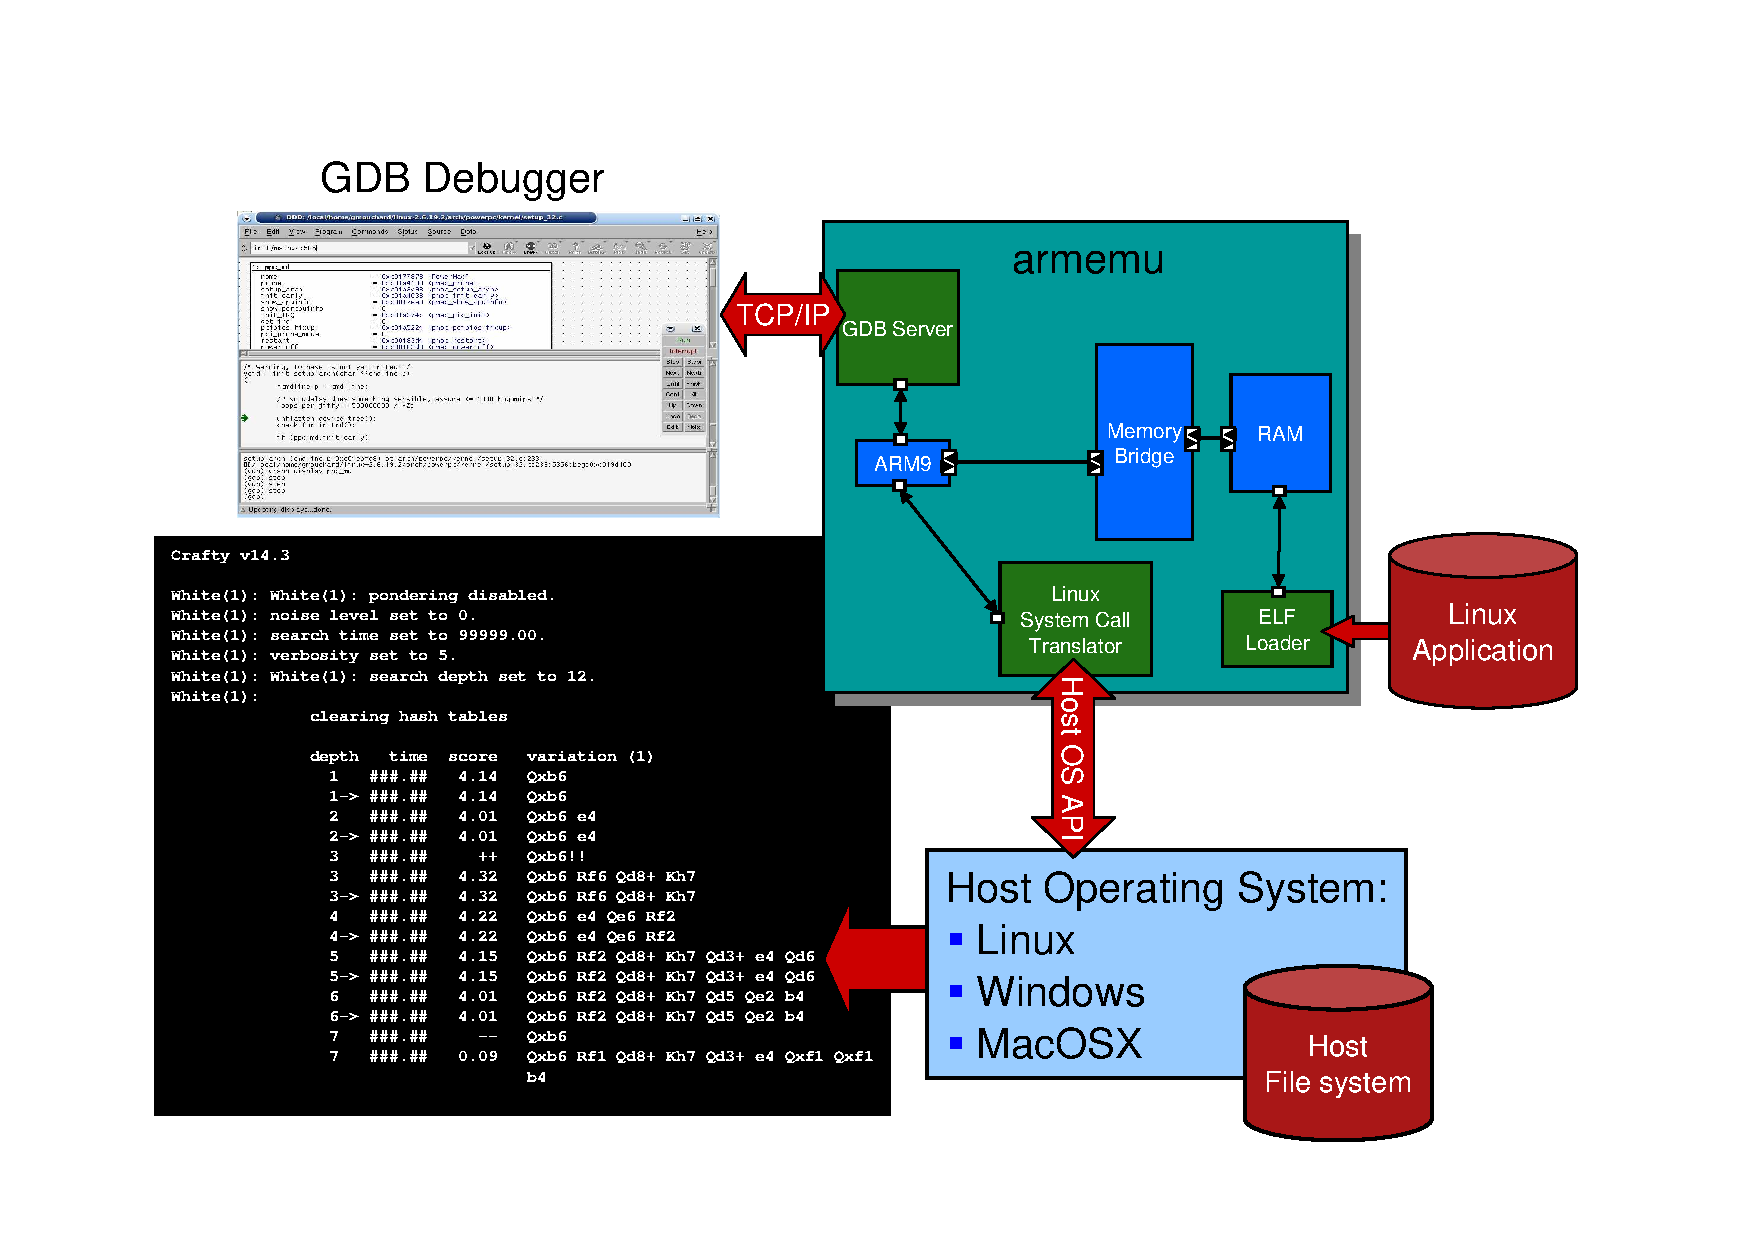
\includegraphics[width=\textwidth]{armemu/fig_schematic.pdf}
	\end{center}
	\caption{UNISIM ARMEmu simulator schematic.}
\end{figure}
\noindent The UNISIM ARMEmu simulator is composed of the following modules and services:
\begin{itemize}\addtolength{\itemsep}{-0.40\baselineskip}
\item \textbf{cpu}
\item \textbf{cpu.dcache}
\item \textbf{cpu.icache}
\item \textbf{debugger}
\item \textbf{gdb-server}: this service implements the GDB server remote serial protocol over TCP/IP. Standards GDB clients (e.g. gdb, eclipse, ddd) can connect to the simulator to debug the target application that runs within the simulator.
\item \textbf{host-time}: this service is an abstraction layer for the host machine time
\item \textbf{inline-debugger}: this service implements a built-in debugger in the terminal console
\item \textbf{linux-os}
\item \textbf{memory}: this module implements a memory
\item \textbf{profiler}
\item \textbf{tee-memory-access-reporting}
\item \textbf{tee-memory-access-reporting.tee-memory-access-reporting.control\_selector[0]}
\item \textbf{tee-memory-access-reporting.tee-memory-access-reporting.control\_selector[10]}
\item \textbf{tee-memory-access-reporting.tee-memory-access-reporting.control\_selector[11]}
\item \textbf{tee-memory-access-reporting.tee-memory-access-reporting.control\_selector[12]}
\item \textbf{tee-memory-access-reporting.tee-memory-access-reporting.control\_selector[13]}
\item \textbf{tee-memory-access-reporting.tee-memory-access-reporting.control\_selector[14]}
\item \textbf{tee-memory-access-reporting.tee-memory-access-reporting.control\_selector[15]}
\item \textbf{tee-memory-access-reporting.tee-memory-access-reporting.control\_selector[1]}
\item \textbf{tee-memory-access-reporting.tee-memory-access-reporting.control\_selector[2]}
\item \textbf{tee-memory-access-reporting.tee-memory-access-reporting.control\_selector[3]}
\item \textbf{tee-memory-access-reporting.tee-memory-access-reporting.control\_selector[4]}
\item \textbf{tee-memory-access-reporting.tee-memory-access-reporting.control\_selector[5]}
\item \textbf{tee-memory-access-reporting.tee-memory-access-reporting.control\_selector[6]}
\item \textbf{tee-memory-access-reporting.tee-memory-access-reporting.control\_selector[7]}
\item \textbf{tee-memory-access-reporting.tee-memory-access-reporting.control\_selector[8]}
\item \textbf{tee-memory-access-reporting.tee-memory-access-reporting.control\_selector[9]}
\item \textbf{time}: this service is an abstraction layer for the SystemC kernel time
\end{itemize}
\subsection{Using the UNISIM ARMEmu simulator}
\label{UNISIM ARMEmu_using}
The UNISIM ARMEmu simulator has the following command line options:\\
~\\
\noindent Usage: \texttt{unisim-armemu-0.7.1 [<options>] [...]}

\noindent Options:
\begin{itemize}
\item \texttt{--set $<$param=value$>$ or -s $<$param=value$>$}: set value of parameter 'param' to 'value'
\item \texttt{--config $<$XML file$>$ or -c $<$XML file$>$}: configures the simulator with the given XML configuration file
\item \texttt{--get-config $<$XML file$>$ or -g $<$XML file$>$}: get the simulator configuration XML file (you can use it to create your own configuration. This option can be combined with -c to get a new configuration file with existing variables from another file
\item \texttt{--list or -l}: lists all available parameters, their type, and their current value
\item \texttt{--warn or -w}: enable printing of kernel warnings
\item \texttt{--doc $<$Latex file$>$ or -d $<$Latex file$>$}: enable printing a latex documentation
\item \texttt{--version or -v}: displays the program version information
\item \texttt{--share-path $<$path$>$ or -p $<$path$>$}: the path that should be used for the share directory (absolute path)
\item \texttt{--help or -h}: displays this help
\end{itemize}
\subsection{Configuration}
\label{UNISIM ARMEmu_configuration}
Simulator configuration (see below) can be modified using command line Options \texttt{--set $<$param=value$>$} or \texttt{--config $<$config file$>$}.\\
~\\
\tablehead{\hline}
\tabletail{\hline}
\begin{supertabular}{|p{7.5cm}|p{7.5cm}|}
\multicolumn{2}{|l|}{\textbf{\Large Global}}\\
\hline
\multicolumn{1}{|p{7.5cm}}{\textbf{Name:} \texttt{enable-gdb-server}} & \multicolumn{1}{p{7.5cm}|}{\textbf{Type:} \texttt{parameter}}\\
\multicolumn{1}{|p{7.5cm}}{\textbf{Default:} \texttt{true}} & \multicolumn{1}{p{7.5cm}|}{\textbf{Data type:} \texttt{boolean}}\\
\multicolumn{2}{|p{15cm}|}{\textbf{Valid:} \texttt{true},~\texttt{false}}\\
\multicolumn{2}{|l|}{}\\
\multicolumn{2}{|p{15cm}|}{\textbf{Description:} \newline Enable GDB server..}\\
\hline
\multicolumn{1}{|p{7.5cm}}{\textbf{Name:} \texttt{enable-inline-debugger}} & \multicolumn{1}{p{7.5cm}|}{\textbf{Type:} \texttt{parameter}}\\
\multicolumn{1}{|p{7.5cm}}{\textbf{Default:} \texttt{true}} & \multicolumn{1}{p{7.5cm}|}{\textbf{Data type:} \texttt{boolean}}\\
\multicolumn{2}{|p{15cm}|}{\textbf{Valid:} \texttt{true},~\texttt{false}}\\
\multicolumn{2}{|l|}{}\\
\multicolumn{2}{|p{15cm}|}{\textbf{Description:} \newline Enable inline debugger..}\\
\hline
\multicolumn{1}{|p{7.5cm}}{\textbf{Name:} \texttt{enable-power-estimation}} & \multicolumn{1}{p{7.5cm}|}{\textbf{Type:} \texttt{parameter}}\\
\multicolumn{1}{|p{7.5cm}}{\textbf{Default:} \texttt{false}} & \multicolumn{1}{p{7.5cm}|}{\textbf{Data type:} \texttt{boolean}}\\
\multicolumn{2}{|p{15cm}|}{\textbf{Valid:} \texttt{true},~\texttt{false}}\\
\multicolumn{2}{|l|}{}\\
\multicolumn{2}{|p{15cm}|}{\textbf{Description:} \newline Activate caches power estimation..}\\
\hline
\multicolumn{1}{|p{7.5cm}}{\textbf{Name:} \texttt{enable-press-enter-at-exit}} & \multicolumn{1}{p{7.5cm}|}{\textbf{Type:} \texttt{parameter}}\\
\multicolumn{1}{|p{7.5cm}}{\textbf{Default:} \texttt{false}} & \multicolumn{1}{p{7.5cm}|}{\textbf{Data type:} \texttt{boolean}}\\
\multicolumn{2}{|p{15cm}|}{\textbf{Valid:} \texttt{true},~\texttt{false}}\\
\multicolumn{2}{|l|}{}\\
\multicolumn{2}{|p{15cm}|}{\textbf{Description:} \newline Enable/Disable pressing key enter at exit.}\\
\hline
\multicolumn{1}{|p{7.5cm}}{\textbf{Name:} \texttt{kernel\_logger.file}} & \multicolumn{1}{p{7.5cm}|}{\textbf{Type:} \texttt{parameter}}\\
\multicolumn{1}{|p{7.5cm}}{\textbf{Default:} \texttt{false}} & \multicolumn{1}{p{7.5cm}|}{\textbf{Data type:} \texttt{boolean}}\\
\multicolumn{2}{|p{15cm}|}{\textbf{Valid:} \texttt{true},~\texttt{false}}\\
\multicolumn{2}{|l|}{}\\
\multicolumn{2}{|p{15cm}|}{\textbf{Description:} \newline Keep logger output in a file.}\\
\hline
\multicolumn{1}{|p{7.5cm}}{\textbf{Name:} \texttt{kernel\_logger.filename}} & \multicolumn{1}{p{7.5cm}|}{\textbf{Type:} \texttt{parameter}}\\
\multicolumn{1}{|p{7.5cm}}{\textbf{Default:} \texttt{logger\_output.txt}} & \multicolumn{1}{p{7.5cm}|}{\textbf{Data type:} \texttt{string}}\\
\multicolumn{2}{|l|}{}\\
\multicolumn{2}{|l|}{}\\
\multicolumn{2}{|p{15cm}|}{\textbf{Description:} \newline Filename to keep logger output \_(the option file must be activated).}\\
\hline
\multicolumn{1}{|p{7.5cm}}{\textbf{Name:} \texttt{kernel\_logger.std\_err}} & \multicolumn{1}{p{7.5cm}|}{\textbf{Type:} \texttt{parameter}}\\
\multicolumn{1}{|p{7.5cm}}{\textbf{Default:} \texttt{true}} & \multicolumn{1}{p{7.5cm}|}{\textbf{Data type:} \texttt{boolean}}\\
\multicolumn{2}{|p{15cm}|}{\textbf{Valid:} \texttt{true},~\texttt{false}}\\
\multicolumn{2}{|l|}{}\\
\multicolumn{2}{|p{15cm}|}{\textbf{Description:} \newline Show logger output through the standard error output.}\\
\hline
\multicolumn{1}{|p{7.5cm}}{\textbf{Name:} \texttt{kernel\_logger.std\_err\_color}} & \multicolumn{1}{p{7.5cm}|}{\textbf{Type:} \texttt{parameter}}\\
\multicolumn{1}{|p{7.5cm}}{\textbf{Default:} \texttt{true}} & \multicolumn{1}{p{7.5cm}|}{\textbf{Data type:} \texttt{boolean}}\\
\multicolumn{2}{|p{15cm}|}{\textbf{Valid:} \texttt{true},~\texttt{false}}\\
\multicolumn{2}{|l|}{}\\
\multicolumn{2}{|p{15cm}|}{\textbf{Description:} \newline Colorize logger output through the standard error output \_(only works if std\_err is active).}\\
\hline
\multicolumn{1}{|p{7.5cm}}{\textbf{Name:} \texttt{kernel\_logger.std\_out}} & \multicolumn{1}{p{7.5cm}|}{\textbf{Type:} \texttt{parameter}}\\
\multicolumn{1}{|p{7.5cm}}{\textbf{Default:} \texttt{false}} & \multicolumn{1}{p{7.5cm}|}{\textbf{Data type:} \texttt{boolean}}\\
\multicolumn{2}{|p{15cm}|}{\textbf{Valid:} \texttt{true},~\texttt{false}}\\
\multicolumn{2}{|l|}{}\\
\multicolumn{2}{|p{15cm}|}{\textbf{Description:} \newline Show logger output through the standard output.}\\
\hline
\multicolumn{1}{|p{7.5cm}}{\textbf{Name:} \texttt{kernel\_logger.std\_out\_color}} & \multicolumn{1}{p{7.5cm}|}{\textbf{Type:} \texttt{parameter}}\\
\multicolumn{1}{|p{7.5cm}}{\textbf{Default:} \texttt{false}} & \multicolumn{1}{p{7.5cm}|}{\textbf{Data type:} \texttt{boolean}}\\
\multicolumn{2}{|p{15cm}|}{\textbf{Valid:} \texttt{true},~\texttt{false}}\\
\multicolumn{2}{|l|}{}\\
\multicolumn{2}{|p{15cm}|}{\textbf{Description:} \newline Colorize logger output through the standard output \_(only works if std\_out is active).}\\
\hline
\multicolumn{1}{|p{7.5cm}}{\textbf{Name:} \texttt{kernel\_logger.xml\_file}} & \multicolumn{1}{p{7.5cm}|}{\textbf{Type:} \texttt{parameter}}\\
\multicolumn{1}{|p{7.5cm}}{\textbf{Default:} \texttt{false}} & \multicolumn{1}{p{7.5cm}|}{\textbf{Data type:} \texttt{boolean}}\\
\multicolumn{2}{|p{15cm}|}{\textbf{Valid:} \texttt{true},~\texttt{false}}\\
\multicolumn{2}{|l|}{}\\
\multicolumn{2}{|p{15cm}|}{\textbf{Description:} \newline Keep logger output in a file xml formatted.}\\
\hline
\multicolumn{1}{|p{7.5cm}}{\textbf{Name:} \texttt{kernel\_logger.xml\_file\_gzipped}} & \multicolumn{1}{p{7.5cm}|}{\textbf{Type:} \texttt{parameter}}\\
\multicolumn{1}{|p{7.5cm}}{\textbf{Default:} \texttt{false}} & \multicolumn{1}{p{7.5cm}|}{\textbf{Data type:} \texttt{boolean}}\\
\multicolumn{2}{|p{15cm}|}{\textbf{Valid:} \texttt{true},~\texttt{false}}\\
\multicolumn{2}{|l|}{}\\
\multicolumn{2}{|p{15cm}|}{\textbf{Description:} \newline If the xml\_file option is active, the output file will be compressed (a .gz extension will be automatically added to the xml\_filename option.}\\
\hline
\multicolumn{1}{|p{7.5cm}}{\textbf{Name:} \texttt{kernel\_logger.xml\_filename}} & \multicolumn{1}{p{7.5cm}|}{\textbf{Type:} \texttt{parameter}}\\
\multicolumn{1}{|p{7.5cm}}{\textbf{Default:} \texttt{logger\_output.xml}} & \multicolumn{1}{p{7.5cm}|}{\textbf{Data type:} \texttt{string}}\\
\multicolumn{2}{|l|}{}\\
\multicolumn{2}{|l|}{}\\
\multicolumn{2}{|p{15cm}|}{\textbf{Description:} \newline Filename to keep logger xml output \_(the option xml\_file must be activated).}\\
\hline
\hline
\multicolumn{2}{|l|}{\textbf{\Large cpu}}\\
\hline
\multicolumn{1}{|p{7.5cm}}{\textbf{Name:} \texttt{cpu.default-endianness}} & \multicolumn{1}{p{7.5cm}|}{\textbf{Type:} \texttt{parameter}}\\
\multicolumn{1}{|p{7.5cm}}{\textbf{Default:} \texttt{little-endian}} & \multicolumn{1}{p{7.5cm}|}{\textbf{Data type:} \texttt{string}}\\
\multicolumn{2}{|l|}{}\\
\multicolumn{2}{|l|}{}\\
\multicolumn{2}{|p{15cm}|}{\textbf{Description:} \newline The processor default/boot endianness. Available values are: little-endian and big-endian..}\\
\hline
\multicolumn{1}{|p{7.5cm}}{\textbf{Name:} \texttt{cpu.voltage}} & \multicolumn{1}{p{7.5cm}|}{\textbf{Type:} \texttt{parameter}}\\
\multicolumn{1}{|p{7.5cm}}{\textbf{Default:} \texttt{1800}} & \multicolumn{1}{p{7.5cm}|}{\textbf{Data type:} \texttt{unsigned 64-bit integer}}\\
\multicolumn{2}{|l|}{}\\
\multicolumn{2}{|l|}{}\\
\multicolumn{2}{|p{15cm}|}{\textbf{Description:} \newline The processor voltage in mV..}\\
\hline
\multicolumn{1}{|p{7.5cm}}{\textbf{Name:} \texttt{cpu.verbose}} & \multicolumn{1}{p{7.5cm}|}{\textbf{Type:} \texttt{parameter}}\\
\multicolumn{1}{|p{7.5cm}}{\textbf{Default:} \texttt{0x00000000}} & \multicolumn{1}{p{7.5cm}|}{\textbf{Data type:} \texttt{unsigned 32-bit integer}}\\
\multicolumn{2}{|l|}{}\\
\multicolumn{2}{|l|}{}\\
\multicolumn{2}{|p{15cm}|}{\textbf{Description:} \newline Activate the verbose system (0 = inactive, different than 0 = active)..}\\
\hline
\multicolumn{1}{|p{7.5cm}}{\textbf{Name:} \texttt{cpu.trap-on-instruction-counter}} & \multicolumn{1}{p{7.5cm}|}{\textbf{Type:} \texttt{parameter}}\\
\multicolumn{1}{|p{7.5cm}}{\textbf{Default:} \texttt{0}} & \multicolumn{1}{p{7.5cm}|}{\textbf{Data type:} \texttt{unsigned 64-bit integer}}\\
\multicolumn{2}{|l|}{}\\
\multicolumn{2}{|l|}{}\\
\multicolumn{2}{|p{15cm}|}{\textbf{Description:} \newline Produce a trap when the given instruction count is reached..}\\
\hline
\multicolumn{1}{|p{7.5cm}}{\textbf{Name:} \texttt{cpu.cpu-cycle-time}} & \multicolumn{1}{p{7.5cm}|}{\textbf{Type:} \texttt{parameter}}\\
\multicolumn{1}{|p{7.5cm}}{\textbf{Default:} \texttt{31250 ps}} & \multicolumn{1}{p{7.5cm}|}{\textbf{Data type:} \texttt{sc\_time}}\\
\multicolumn{2}{|l|}{}\\
\multicolumn{2}{|l|}{}\\
\multicolumn{2}{|p{15cm}|}{\textbf{Description:} \newline The processor cycle time..}\\
\hline
\multicolumn{1}{|p{7.5cm}}{\textbf{Name:} \texttt{cpu.bus-cycle-time}} & \multicolumn{1}{p{7.5cm}|}{\textbf{Type:} \texttt{parameter}}\\
\multicolumn{1}{|p{7.5cm}}{\textbf{Default:} \texttt{31250 ps}} & \multicolumn{1}{p{7.5cm}|}{\textbf{Data type:} \texttt{sc\_time}}\\
\multicolumn{2}{|l|}{}\\
\multicolumn{2}{|l|}{}\\
\multicolumn{2}{|p{15cm}|}{\textbf{Description:} \newline The processor bus cycle time..}\\
\hline
\multicolumn{1}{|p{7.5cm}}{\textbf{Name:} \texttt{cpu.nice-time}} & \multicolumn{1}{p{7.5cm}|}{\textbf{Type:} \texttt{parameter}}\\
\multicolumn{1}{|p{7.5cm}}{\textbf{Default:} \texttt{1 ms}} & \multicolumn{1}{p{7.5cm}|}{\textbf{Data type:} \texttt{sc\_time}}\\
\multicolumn{2}{|l|}{}\\
\multicolumn{2}{|l|}{}\\
\multicolumn{2}{|p{15cm}|}{\textbf{Description:} \newline Maximum time between SystemC waits..}\\
\hline
\multicolumn{1}{|p{7.5cm}}{\textbf{Name:} \texttt{cpu.ipc}} & \multicolumn{1}{p{7.5cm}|}{\textbf{Type:} \texttt{parameter}}\\
\multicolumn{1}{|p{7.5cm}}{\textbf{Default:} \texttt{1}} & \multicolumn{1}{p{7.5cm}|}{\textbf{Data type:} \texttt{double precision floating-point}}\\
\multicolumn{2}{|l|}{}\\
\multicolumn{2}{|l|}{}\\
\multicolumn{2}{|p{15cm}|}{\textbf{Description:} \newline Instructions per cycle performance..}\\
\hline
\multicolumn{1}{|p{7.5cm}}{\textbf{Name:} \texttt{cpu.verbose-tlm}} & \multicolumn{1}{p{7.5cm}|}{\textbf{Type:} \texttt{parameter}}\\
\multicolumn{1}{|p{7.5cm}}{\textbf{Default:} \texttt{false}} & \multicolumn{1}{p{7.5cm}|}{\textbf{Data type:} \texttt{boolean}}\\
\multicolumn{2}{|p{15cm}|}{\textbf{Valid:} \texttt{true},~\texttt{false}}\\
\multicolumn{2}{|l|}{}\\
\multicolumn{2}{|p{15cm}|}{\textbf{Description:} \newline Display TLM information.}\\
\hline
\hline
\multicolumn{2}{|l|}{\textbf{\Large cpu.dcache}}\\
\hline
\multicolumn{1}{|p{7.5cm}}{\textbf{Name:} \texttt{cpu.dcache.size}} & \multicolumn{1}{p{7.5cm}|}{\textbf{Type:} \texttt{parameter}}\\
\multicolumn{1}{|p{7.5cm}}{\textbf{Default:} \texttt{131072}} & \multicolumn{1}{p{7.5cm}|}{\textbf{Data type:} \texttt{unsigned 32-bit integer}}\\
\multicolumn{2}{|l|}{}\\
\multicolumn{2}{|l|}{}\\
\multicolumn{2}{|p{15cm}|}{\textbf{Description:} \newline Size of the cache in bytes. Avalaible sizes are 4KB, 8KB, 16KB, 32KB, 64KB and 128KB. The cache can be deactivated setting this value to 0..}\\
\hline
\hline
\multicolumn{2}{|l|}{\textbf{\Large cpu.icache}}\\
\hline
\multicolumn{1}{|p{7.5cm}}{\textbf{Name:} \texttt{cpu.icache.size}} & \multicolumn{1}{p{7.5cm}|}{\textbf{Type:} \texttt{parameter}}\\
\multicolumn{1}{|p{7.5cm}}{\textbf{Default:} \texttt{131072}} & \multicolumn{1}{p{7.5cm}|}{\textbf{Data type:} \texttt{unsigned 32-bit integer}}\\
\multicolumn{2}{|l|}{}\\
\multicolumn{2}{|l|}{}\\
\multicolumn{2}{|p{15cm}|}{\textbf{Description:} \newline Size of the cache in bytes. Avalaible sizes are 4KB, 8KB, 16KB, 32KB, 64KB and 128KB. The cache can be deactivated setting this value to 0..}\\
\hline
\hline
\multicolumn{2}{|l|}{\textbf{\Large debugger}}\\
\hline
\multicolumn{1}{|p{7.5cm}}{\textbf{Name:} \texttt{debugger.verbose}} & \multicolumn{1}{p{7.5cm}|}{\textbf{Type:} \texttt{parameter}}\\
\multicolumn{1}{|p{7.5cm}}{\textbf{Default:} \texttt{false}} & \multicolumn{1}{p{7.5cm}|}{\textbf{Data type:} \texttt{boolean}}\\
\multicolumn{2}{|p{15cm}|}{\textbf{Valid:} \texttt{true},~\texttt{false}}\\
\multicolumn{2}{|l|}{}\\
\multicolumn{2}{|p{15cm}|}{\textbf{Description:} \newline Enable/Disable verbosity.}\\
\hline
\multicolumn{1}{|p{7.5cm}}{\textbf{Name:} \texttt{debugger.dwarf-to-html-output-} \newline$\hookrightarrow$\texttt{directory}} & \multicolumn{1}{p{7.5cm}|}{\textbf{Type:} \texttt{parameter}}\\
\multicolumn{1}{|p{7.5cm}}{\textbf{Default:} \texttt{}} & \multicolumn{1}{p{7.5cm}|}{\textbf{Data type:} \texttt{string}}\\
\multicolumn{2}{|l|}{}\\
\multicolumn{2}{|l|}{}\\
\multicolumn{2}{|p{15cm}|}{\textbf{Description:} \newline DWARF v2/v3 to HTML output directory.}\\
\hline
\multicolumn{1}{|p{7.5cm}}{\textbf{Name:} \texttt{debugger.dwarf-register-number-} \newline$\hookrightarrow$\texttt{mapping-filename}} & \multicolumn{1}{p{7.5cm}|}{\textbf{Type:} \texttt{parameter}}\\
\multicolumn{1}{|p{7.5cm}}{\textbf{Default:} \texttt{arm\_eabi\_dwarf\_register\_} \newline$\hookrightarrow$\texttt{number\_mapping.xml}} & \multicolumn{1}{p{7.5cm}|}{\textbf{Data type:} \texttt{string}}\\
\multicolumn{2}{|l|}{}\\
\multicolumn{2}{|l|}{}\\
\multicolumn{2}{|p{15cm}|}{\textbf{Description:} \newline DWARF register number mapping filename.}\\
\hline
\multicolumn{1}{|p{7.5cm}}{\textbf{Name:} \texttt{debugger.parse-dwarf}} & \multicolumn{1}{p{7.5cm}|}{\textbf{Type:} \texttt{parameter}}\\
\multicolumn{1}{|p{7.5cm}}{\textbf{Default:} \texttt{true}} & \multicolumn{1}{p{7.5cm}|}{\textbf{Data type:} \texttt{boolean}}\\
\multicolumn{2}{|p{15cm}|}{\textbf{Valid:} \texttt{true},~\texttt{false}}\\
\multicolumn{2}{|l|}{}\\
\multicolumn{2}{|p{15cm}|}{\textbf{Description:} \newline Enable/Disable parsing of DWARF debugging informations.}\\
\hline
\multicolumn{1}{|p{7.5cm}}{\textbf{Name:} \texttt{debugger.debug-dwarf}} & \multicolumn{1}{p{7.5cm}|}{\textbf{Type:} \texttt{parameter}}\\
\multicolumn{1}{|p{7.5cm}}{\textbf{Default:} \texttt{false}} & \multicolumn{1}{p{7.5cm}|}{\textbf{Data type:} \texttt{boolean}}\\
\multicolumn{2}{|p{15cm}|}{\textbf{Valid:} \texttt{true},~\texttt{false}}\\
\multicolumn{2}{|l|}{}\\
\multicolumn{2}{|p{15cm}|}{\textbf{Description:} \newline Enable/Disable debugging of DWARF.}\\
\hline
\hline
\multicolumn{2}{|l|}{\textbf{\Large gdb-server}}\\
\hline
\multicolumn{1}{|p{7.5cm}}{\textbf{Name:} \texttt{gdb-server.memory-atom-size}} & \multicolumn{1}{p{7.5cm}|}{\textbf{Type:} \texttt{parameter}}\\
\multicolumn{1}{|p{7.5cm}}{\textbf{Default:} \texttt{0x00000001}} & \multicolumn{1}{p{7.5cm}|}{\textbf{Data type:} \texttt{unsigned 32-bit integer}}\\
\multicolumn{2}{|l|}{}\\
\multicolumn{2}{|l|}{}\\
\multicolumn{2}{|p{15cm}|}{\textbf{Description:} \newline size of the smallest addressable element in memory.}\\
\hline
\multicolumn{1}{|p{7.5cm}}{\textbf{Name:} \texttt{gdb-server.tcp-port}} & \multicolumn{1}{p{7.5cm}|}{\textbf{Type:} \texttt{parameter}}\\
\multicolumn{1}{|p{7.5cm}}{\textbf{Default:} \texttt{12345}} & \multicolumn{1}{p{7.5cm}|}{\textbf{Data type:} \texttt{signed 32-bit integer}}\\
\multicolumn{2}{|l|}{}\\
\multicolumn{2}{|l|}{}\\
\multicolumn{2}{|p{15cm}|}{\textbf{Description:} \newline TCP/IP port to listen waiting for a GDB client connection.}\\
\hline
\multicolumn{1}{|p{7.5cm}}{\textbf{Name:} \texttt{gdb-server.architecture-description-} \newline$\hookrightarrow$\texttt{filename}} & \multicolumn{1}{p{7.5cm}|}{\textbf{Type:} \texttt{parameter}}\\
\multicolumn{1}{|p{7.5cm}}{\textbf{Default:} \texttt{gdb\_armv5l.xml}} & \multicolumn{1}{p{7.5cm}|}{\textbf{Data type:} \texttt{string}}\\
\multicolumn{2}{|l|}{}\\
\multicolumn{2}{|l|}{}\\
\multicolumn{2}{|p{15cm}|}{\textbf{Description:} \newline filename of a XML description of the connected processor.}\\
\hline
\multicolumn{1}{|p{7.5cm}}{\textbf{Name:} \texttt{gdb-server.verbose}} & \multicolumn{1}{p{7.5cm}|}{\textbf{Type:} \texttt{parameter}}\\
\multicolumn{1}{|p{7.5cm}}{\textbf{Default:} \texttt{false}} & \multicolumn{1}{p{7.5cm}|}{\textbf{Data type:} \texttt{boolean}}\\
\multicolumn{2}{|p{15cm}|}{\textbf{Valid:} \texttt{true},~\texttt{false}}\\
\multicolumn{2}{|l|}{}\\
\multicolumn{2}{|p{15cm}|}{\textbf{Description:} \newline Enable/Disable verbosity.}\\
\hline
\hline
\multicolumn{2}{|l|}{\textbf{\Large inline-debugger}}\\
\hline
\multicolumn{1}{|p{7.5cm}}{\textbf{Name:} \texttt{inline-debugger.memory-atom-} \newline$\hookrightarrow$\texttt{size}} & \multicolumn{1}{p{7.5cm}|}{\textbf{Type:} \texttt{parameter}}\\
\multicolumn{1}{|p{7.5cm}}{\textbf{Default:} \texttt{0x00000001}} & \multicolumn{1}{p{7.5cm}|}{\textbf{Data type:} \texttt{unsigned 32-bit integer}}\\
\multicolumn{2}{|l|}{}\\
\multicolumn{2}{|l|}{}\\
\multicolumn{2}{|p{15cm}|}{\textbf{Description:} \newline size of the smallest addressable element in memory.}\\
\hline
\multicolumn{1}{|p{7.5cm}}{\textbf{Name:} \texttt{inline-debugger.search-path}} & \multicolumn{1}{p{7.5cm}|}{\textbf{Type:} \texttt{parameter}}\\
\multicolumn{1}{|p{7.5cm}}{\textbf{Default:} \texttt{}} & \multicolumn{1}{p{7.5cm}|}{\textbf{Data type:} \texttt{string}}\\
\multicolumn{2}{|l|}{}\\
\multicolumn{2}{|l|}{}\\
\multicolumn{2}{|p{15cm}|}{\textbf{Description:} \newline Search path for source (separated by ';').}\\
\hline
\multicolumn{1}{|p{7.5cm}}{\textbf{Name:} \texttt{inline-debugger.init-macro}} & \multicolumn{1}{p{7.5cm}|}{\textbf{Type:} \texttt{parameter}}\\
\multicolumn{1}{|p{7.5cm}}{\textbf{Default:} \texttt{}} & \multicolumn{1}{p{7.5cm}|}{\textbf{Data type:} \texttt{string}}\\
\multicolumn{2}{|l|}{}\\
\multicolumn{2}{|l|}{}\\
\multicolumn{2}{|p{15cm}|}{\textbf{Description:} \newline path to initial macro to run when debugger starts.}\\
\hline
\multicolumn{1}{|p{7.5cm}}{\textbf{Name:} \texttt{inline-debugger.output}} & \multicolumn{1}{p{7.5cm}|}{\textbf{Type:} \texttt{parameter}}\\
\multicolumn{1}{|p{7.5cm}}{\textbf{Default:} \texttt{}} & \multicolumn{1}{p{7.5cm}|}{\textbf{Data type:} \texttt{string}}\\
\multicolumn{2}{|l|}{}\\
\multicolumn{2}{|l|}{}\\
\multicolumn{2}{|p{15cm}|}{\textbf{Description:} \newline path to output file where to redirect the debugger outputs.}\\
\hline
\hline
\multicolumn{2}{|l|}{\textbf{\Large linux-os}}\\
\hline
\multicolumn{1}{|p{7.5cm}}{\textbf{Name:} \texttt{linux-os.verbose}} & \multicolumn{1}{p{7.5cm}|}{\textbf{Type:} \texttt{parameter}}\\
\multicolumn{1}{|p{7.5cm}}{\textbf{Default:} \texttt{false}} & \multicolumn{1}{p{7.5cm}|}{\textbf{Data type:} \texttt{boolean}}\\
\multicolumn{2}{|p{15cm}|}{\textbf{Valid:} \texttt{true},~\texttt{false}}\\
\hline
\multicolumn{1}{|p{7.5cm}}{\textbf{Name:} \texttt{linux-os.parse-dwarf}} & \multicolumn{1}{p{7.5cm}|}{\textbf{Type:} \texttt{parameter}}\\
\multicolumn{1}{|p{7.5cm}}{\textbf{Default:} \texttt{false}} & \multicolumn{1}{p{7.5cm}|}{\textbf{Data type:} \texttt{boolean}}\\
\multicolumn{2}{|p{15cm}|}{\textbf{Valid:} \texttt{true},~\texttt{false}}\\
\hline
\multicolumn{1}{|p{7.5cm}}{\textbf{Name:} \texttt{linux-os.debug-dwarf}} & \multicolumn{1}{p{7.5cm}|}{\textbf{Type:} \texttt{parameter}}\\
\multicolumn{1}{|p{7.5cm}}{\textbf{Default:} \texttt{false}} & \multicolumn{1}{p{7.5cm}|}{\textbf{Data type:} \texttt{boolean}}\\
\multicolumn{2}{|p{15cm}|}{\textbf{Valid:} \texttt{true},~\texttt{false}}\\
\hline
\multicolumn{1}{|p{7.5cm}}{\textbf{Name:} \texttt{linux-os.dwarf-to-html-output-} \newline$\hookrightarrow$\texttt{directory}} & \multicolumn{1}{p{7.5cm}|}{\textbf{Type:} \texttt{parameter}}\\
\multicolumn{1}{|p{7.5cm}}{\textbf{Default:} \texttt{}} & \multicolumn{1}{p{7.5cm}|}{\textbf{Data type:} \texttt{string}}\\
\multicolumn{2}{|l|}{}\\
\hline
\multicolumn{1}{|p{7.5cm}}{\textbf{Name:} \texttt{linux-os.dwarf-to-xml-output-} \newline$\hookrightarrow$\texttt{filename}} & \multicolumn{1}{p{7.5cm}|}{\textbf{Type:} \texttt{parameter}}\\
\multicolumn{1}{|p{7.5cm}}{\textbf{Default:} \texttt{}} & \multicolumn{1}{p{7.5cm}|}{\textbf{Data type:} \texttt{string}}\\
\multicolumn{2}{|l|}{}\\
\hline
\multicolumn{1}{|p{7.5cm}}{\textbf{Name:} \texttt{linux-os.system}} & \multicolumn{1}{p{7.5cm}|}{\textbf{Type:} \texttt{parameter}}\\
\multicolumn{1}{|p{7.5cm}}{\textbf{Default:} \texttt{arm-eabi}} & \multicolumn{1}{p{7.5cm}|}{\textbf{Data type:} \texttt{string}}\\
\multicolumn{2}{|l|}{}\\
\multicolumn{2}{|l|}{}\\
\multicolumn{2}{|p{15cm}|}{\textbf{Description:} \newline Emulated system architecture available values are "arm", "arm-eabi" and "powerpc".}\\
\hline
\multicolumn{1}{|p{7.5cm}}{\textbf{Name:} \texttt{linux-os.endianness}} & \multicolumn{1}{p{7.5cm}|}{\textbf{Type:} \texttt{parameter}}\\
\multicolumn{1}{|p{7.5cm}}{\textbf{Default:} \texttt{little-endian}} & \multicolumn{1}{p{7.5cm}|}{\textbf{Data type:} \texttt{endianess}}\\
\multicolumn{2}{|p{15cm}|}{\textbf{Valid:} \texttt{little-endian},~\texttt{big-endian}}\\
\multicolumn{2}{|l|}{}\\
\multicolumn{2}{|p{15cm}|}{\textbf{Description:} \newline The endianness of the binary loaded. Available values are: little-endian and big-endian..}\\
\hline
\multicolumn{1}{|p{7.5cm}}{\textbf{Name:} \texttt{linux-os.memory-page-size}} & \multicolumn{1}{p{7.5cm}|}{\textbf{Type:} \texttt{parameter}}\\
\multicolumn{1}{|p{7.5cm}}{\textbf{Default:} \texttt{0x00001000}} & \multicolumn{1}{p{7.5cm}|}{\textbf{Data type:} \texttt{unsigned 32-bit integer}}\\
\multicolumn{2}{|l|}{}\\
\hline
\multicolumn{1}{|p{7.5cm}}{\textbf{Name:} \texttt{linux-os.stack-base}} & \multicolumn{1}{p{7.5cm}|}{\textbf{Type:} \texttt{parameter}}\\
\multicolumn{1}{|p{7.5cm}}{\textbf{Default:} \texttt{0x40000000}} & \multicolumn{1}{p{7.5cm}|}{\textbf{Data type:} \texttt{unsigned 32-bit integer}}\\
\multicolumn{2}{|l|}{}\\
\multicolumn{2}{|l|}{}\\
\multicolumn{2}{|p{15cm}|}{\textbf{Description:} \newline The stack base address used for the load and execution of the linux application.}\\
\hline
\multicolumn{1}{|p{7.5cm}}{\textbf{Name:} \texttt{linux-os.binary}} & \multicolumn{1}{p{7.5cm}|}{\textbf{Type:} \texttt{parameter}}\\
\multicolumn{1}{|p{7.5cm}}{\textbf{Default:} \texttt{}} & \multicolumn{1}{p{7.5cm}|}{\textbf{Data type:} \texttt{string}}\\
\multicolumn{2}{|l|}{}\\
\multicolumn{2}{|l|}{}\\
\multicolumn{2}{|p{15cm}|}{\textbf{Description:} \newline The binary to execute on the target simulator. Usually it is the same value than the argv[1] parameter..}\\
\hline
\multicolumn{1}{|p{7.5cm}}{\textbf{Name:} \texttt{linux-os.argc}} & \multicolumn{1}{p{7.5cm}|}{\textbf{Type:} \texttt{parameter}}\\
\multicolumn{1}{|p{7.5cm}}{\textbf{Default:} \texttt{0}} & \multicolumn{1}{p{7.5cm}|}{\textbf{Data type:} \texttt{unsigned 32-bit integer}}\\
\multicolumn{2}{|l|}{}\\
\multicolumn{2}{|l|}{}\\
\multicolumn{2}{|p{15cm}|}{\textbf{Description:} \newline Number of commands in the program execution line (usually at least one which is the name of the program executed). The different tokens can be set up with the parameters argv[$<$n$>$] where $<$n$>$ can go up to argc - 1..}\\
\hline
\multicolumn{1}{|p{7.5cm}}{\textbf{Name:} \texttt{linux-os.apply-host-environment}} & \multicolumn{1}{p{7.5cm}|}{\textbf{Type:} \texttt{parameter}}\\
\multicolumn{1}{|p{7.5cm}}{\textbf{Default:} \texttt{false}} & \multicolumn{1}{p{7.5cm}|}{\textbf{Data type:} \texttt{boolean}}\\
\multicolumn{2}{|p{15cm}|}{\textbf{Valid:} \texttt{true},~\texttt{false}}\\
\multicolumn{2}{|l|}{}\\
\multicolumn{2}{|p{15cm}|}{\textbf{Description:} \newline Wether to apply the host environment on the target simulator or use the provided envc and envp..}\\
\hline
\multicolumn{1}{|p{7.5cm}}{\textbf{Name:} \texttt{linux-os.envc}} & \multicolumn{1}{p{7.5cm}|}{\textbf{Type:} \texttt{parameter}}\\
\multicolumn{1}{|p{7.5cm}}{\textbf{Default:} \texttt{0x00000000}} & \multicolumn{1}{p{7.5cm}|}{\textbf{Data type:} \texttt{unsigned 32-bit integer}}\\
\multicolumn{2}{|l|}{}\\
\multicolumn{2}{|l|}{}\\
\multicolumn{2}{|p{15cm}|}{\textbf{Description:} \newline Number of environment variables defined for the program execution. The different variables can be set up with the parameters envp[$<$n$>$] where $<$n$>$ can go up to envc - 1..}\\
\hline
\multicolumn{1}{|p{7.5cm}}{\textbf{Name:} \texttt{linux-os.utsname-sysname}} & \multicolumn{1}{p{7.5cm}|}{\textbf{Type:} \texttt{parameter}}\\
\multicolumn{1}{|p{7.5cm}}{\textbf{Default:} \texttt{Linux}} & \multicolumn{1}{p{7.5cm}|}{\textbf{Data type:} \texttt{string}}\\
\multicolumn{2}{|l|}{}\\
\multicolumn{2}{|l|}{}\\
\multicolumn{2}{|p{15cm}|}{\textbf{Description:} \newline The value that the uname system call should return. As this service is providing linux emulation supoort its value should be 'Linux', so you should not modify it..}\\
\hline
\multicolumn{1}{|p{7.5cm}}{\textbf{Name:} \texttt{linux-os.utsname-nodename}} & \multicolumn{1}{p{7.5cm}|}{\textbf{Type:} \texttt{parameter}}\\
\multicolumn{1}{|p{7.5cm}}{\textbf{Default:} \texttt{localhost}} & \multicolumn{1}{p{7.5cm}|}{\textbf{Data type:} \texttt{string}}\\
\multicolumn{2}{|l|}{}\\
\multicolumn{2}{|l|}{}\\
\multicolumn{2}{|p{15cm}|}{\textbf{Description:} \newline The network node hostname that the uname system call should return. Default value is localhost, but you could write whatever name you want..}\\
\hline
\multicolumn{1}{|p{7.5cm}}{\textbf{Name:} \texttt{linux-os.utsname-release}} & \multicolumn{1}{p{7.5cm}|}{\textbf{Type:} \texttt{parameter}}\\
\multicolumn{1}{|p{7.5cm}}{\textbf{Default:} \texttt{2.6.27.35}} & \multicolumn{1}{p{7.5cm}|}{\textbf{Data type:} \texttt{string}}\\
\multicolumn{2}{|l|}{}\\
\multicolumn{2}{|l|}{}\\
\multicolumn{2}{|p{15cm}|}{\textbf{Description:} \newline The kernel realese information that the uname system call should return. This should usually match the linux-kernel parameter..}\\
\hline
\multicolumn{1}{|p{7.5cm}}{\textbf{Name:} \texttt{linux-os.utsname-version}} & \multicolumn{1}{p{7.5cm}|}{\textbf{Type:} \texttt{parameter}}\\
\multicolumn{1}{|p{7.5cm}}{\textbf{Default:} \texttt{\#UNISIM SMP Fri Mar 12 05:23:09 } \newline$\hookrightarrow$\texttt{UTC 2010}} & \multicolumn{1}{p{7.5cm}|}{\textbf{Data type:} \texttt{string}}\\
\multicolumn{2}{|l|}{}\\
\multicolumn{2}{|l|}{}\\
\multicolumn{2}{|p{15cm}|}{\textbf{Description:} \newline The kernel version information that the uname system call should return..}\\
\hline
\multicolumn{1}{|p{7.5cm}}{\textbf{Name:} \texttt{linux-os.utsname-machine}} & \multicolumn{1}{p{7.5cm}|}{\textbf{Type:} \texttt{parameter}}\\
\multicolumn{1}{|p{7.5cm}}{\textbf{Default:} \texttt{armv5}} & \multicolumn{1}{p{7.5cm}|}{\textbf{Data type:} \texttt{string}}\\
\multicolumn{2}{|l|}{}\\
\multicolumn{2}{|l|}{}\\
\multicolumn{2}{|p{15cm}|}{\textbf{Description:} \newline The machine information that the uname system call should  return. This should be one of the supported architectures (the  system parameter, that is, arm or powerpc) or a specific model  derived from it (i.e., arm926ejs)..}\\
\hline
\multicolumn{1}{|p{7.5cm}}{\textbf{Name:} \texttt{linux-os.utsname-domainname}} & \multicolumn{1}{p{7.5cm}|}{\textbf{Type:} \texttt{parameter}}\\
\multicolumn{1}{|p{7.5cm}}{\textbf{Default:} \texttt{localhost}} & \multicolumn{1}{p{7.5cm}|}{\textbf{Data type:} \texttt{string}}\\
\multicolumn{2}{|l|}{}\\
\multicolumn{2}{|l|}{}\\
\multicolumn{2}{|p{15cm}|}{\textbf{Description:} \newline The domain name information that the uname system call should return..}\\
\hline
\multicolumn{1}{|p{7.5cm}}{\textbf{Name:} \texttt{linux-os.hwcap}} & \multicolumn{1}{p{7.5cm}|}{\textbf{Type:} \texttt{parameter}}\\
\multicolumn{1}{|p{7.5cm}}{\textbf{Default:} \texttt{swp half fastmult}} & \multicolumn{1}{p{7.5cm}|}{\textbf{Data type:} \texttt{string}}\\
\multicolumn{2}{|l|}{}\\
\multicolumn{2}{|l|}{}\\
\multicolumn{2}{|p{15cm}|}{\textbf{Description:} \newline CPU Hardware capabilities to enable (e.g. "swp thumb fastmult vfp"..}\\
\hline
\hline
\multicolumn{2}{|l|}{\textbf{\Large memory}}\\
\hline
\multicolumn{1}{|p{7.5cm}}{\textbf{Name:} \texttt{memory.org}} & \multicolumn{1}{p{7.5cm}|}{\textbf{Type:} \texttt{parameter}}\\
\multicolumn{1}{|p{7.5cm}}{\textbf{Default:} \texttt{0x00000000}} & \multicolumn{1}{p{7.5cm}|}{\textbf{Data type:} \texttt{unsigned 32-bit integer}}\\
\multicolumn{2}{|l|}{}\\
\multicolumn{2}{|l|}{}\\
\multicolumn{2}{|p{15cm}|}{\textbf{Description:} \newline memory origin/base address.}\\
\hline
\multicolumn{1}{|p{7.5cm}}{\textbf{Name:} \texttt{memory.bytesize}} & \multicolumn{1}{p{7.5cm}|}{\textbf{Type:} \texttt{parameter}}\\
\multicolumn{1}{|p{7.5cm}}{\textbf{Default:} \texttt{4294967295}} & \multicolumn{1}{p{7.5cm}|}{\textbf{Data type:} \texttt{unsigned 32-bit integer}}\\
\multicolumn{2}{|l|}{}\\
\multicolumn{2}{|l|}{}\\
\multicolumn{2}{|p{15cm}|}{\textbf{Description:} \newline memory size in bytes.}\\
\hline
\multicolumn{1}{|p{7.5cm}}{\textbf{Name:} \texttt{memory.initial-byte-value}} & \multicolumn{1}{p{7.5cm}|}{\textbf{Type:} \texttt{parameter}}\\
\multicolumn{1}{|p{7.5cm}}{\textbf{Default:} \texttt{0x00}} & \multicolumn{1}{p{7.5cm}|}{\textbf{Data type:} \texttt{unsigned 8-bit integer}}\\
\multicolumn{2}{|l|}{}\\
\hline
\multicolumn{1}{|p{7.5cm}}{\textbf{Name:} \texttt{memory.cycle-time}} & \multicolumn{1}{p{7.5cm}|}{\textbf{Type:} \texttt{parameter}}\\
\multicolumn{1}{|p{7.5cm}}{\textbf{Default:} \texttt{31250 ps}} & \multicolumn{1}{p{7.5cm}|}{\textbf{Data type:} \texttt{sc\_time}}\\
\multicolumn{2}{|l|}{}\\
\multicolumn{2}{|l|}{}\\
\multicolumn{2}{|p{15cm}|}{\textbf{Description:} \newline memory cycle time.}\\
\hline
\multicolumn{1}{|p{7.5cm}}{\textbf{Name:} \texttt{memory.read-latency}} & \multicolumn{1}{p{7.5cm}|}{\textbf{Type:} \texttt{parameter}}\\
\multicolumn{1}{|p{7.5cm}}{\textbf{Default:} \texttt{31250 ps}} & \multicolumn{1}{p{7.5cm}|}{\textbf{Data type:} \texttt{sc\_time}}\\
\multicolumn{2}{|l|}{}\\
\multicolumn{2}{|l|}{}\\
\multicolumn{2}{|p{15cm}|}{\textbf{Description:} \newline memory read latency.}\\
\hline
\multicolumn{1}{|p{7.5cm}}{\textbf{Name:} \texttt{memory.write-latency}} & \multicolumn{1}{p{7.5cm}|}{\textbf{Type:} \texttt{parameter}}\\
\multicolumn{1}{|p{7.5cm}}{\textbf{Default:} \texttt{0 s}} & \multicolumn{1}{p{7.5cm}|}{\textbf{Data type:} \texttt{sc\_time}}\\
\multicolumn{2}{|l|}{}\\
\multicolumn{2}{|l|}{}\\
\multicolumn{2}{|p{15cm}|}{\textbf{Description:} \newline memory write latency.}\\
\hline
\multicolumn{1}{|p{7.5cm}}{\textbf{Name:} \texttt{memory.verbose}} & \multicolumn{1}{p{7.5cm}|}{\textbf{Type:} \texttt{parameter}}\\
\multicolumn{1}{|p{7.5cm}}{\textbf{Default:} \texttt{false}} & \multicolumn{1}{p{7.5cm}|}{\textbf{Data type:} \texttt{boolean}}\\
\multicolumn{2}{|p{15cm}|}{\textbf{Valid:} \texttt{true},~\texttt{false}}\\
\multicolumn{2}{|l|}{}\\
\multicolumn{2}{|p{15cm}|}{\textbf{Description:} \newline enable/disable verbosity.}\\
\hline
\hline
\multicolumn{2}{|l|}{\textbf{\Large profiler}}\\
\hline
\multicolumn{1}{|p{7.5cm}}{\textbf{Name:} \texttt{profiler.min-data-read-prof-} \newline$\hookrightarrow$\texttt{addr}} & \multicolumn{1}{p{7.5cm}|}{\textbf{Type:} \texttt{parameter}}\\
\multicolumn{1}{|p{7.5cm}}{\textbf{Default:} \texttt{0x00000000}} & \multicolumn{1}{p{7.5cm}|}{\textbf{Data type:} \texttt{unsigned 32-bit integer}}\\
\multicolumn{2}{|l|}{}\\
\multicolumn{2}{|l|}{}\\
\multicolumn{2}{|p{15cm}|}{\textbf{Description:} \newline Minimum address for data read profiling.}\\
\hline
\multicolumn{1}{|p{7.5cm}}{\textbf{Name:} \texttt{profiler.max-data-read-prof-} \newline$\hookrightarrow$\texttt{addr}} & \multicolumn{1}{p{7.5cm}|}{\textbf{Type:} \texttt{parameter}}\\
\multicolumn{1}{|p{7.5cm}}{\textbf{Default:} \texttt{0xffffffff}} & \multicolumn{1}{p{7.5cm}|}{\textbf{Data type:} \texttt{unsigned 32-bit integer}}\\
\multicolumn{2}{|l|}{}\\
\multicolumn{2}{|l|}{}\\
\multicolumn{2}{|p{15cm}|}{\textbf{Description:} \newline Maximum address for data read profiling.}\\
\hline
\multicolumn{1}{|p{7.5cm}}{\textbf{Name:} \texttt{profiler.min-data-write-prof-} \newline$\hookrightarrow$\texttt{addr}} & \multicolumn{1}{p{7.5cm}|}{\textbf{Type:} \texttt{parameter}}\\
\multicolumn{1}{|p{7.5cm}}{\textbf{Default:} \texttt{0x00000000}} & \multicolumn{1}{p{7.5cm}|}{\textbf{Data type:} \texttt{unsigned 32-bit integer}}\\
\multicolumn{2}{|l|}{}\\
\multicolumn{2}{|l|}{}\\
\multicolumn{2}{|p{15cm}|}{\textbf{Description:} \newline Minimum address for data write profiling.}\\
\hline
\multicolumn{1}{|p{7.5cm}}{\textbf{Name:} \texttt{profiler.max-data-write-prof-} \newline$\hookrightarrow$\texttt{addr}} & \multicolumn{1}{p{7.5cm}|}{\textbf{Type:} \texttt{parameter}}\\
\multicolumn{1}{|p{7.5cm}}{\textbf{Default:} \texttt{0xffffffff}} & \multicolumn{1}{p{7.5cm}|}{\textbf{Data type:} \texttt{unsigned 32-bit integer}}\\
\multicolumn{2}{|l|}{}\\
\multicolumn{2}{|l|}{}\\
\multicolumn{2}{|p{15cm}|}{\textbf{Description:} \newline Maximum address for data write profiling.}\\
\hline
\multicolumn{1}{|p{7.5cm}}{\textbf{Name:} \texttt{profiler.min-insn-fetch-prof-} \newline$\hookrightarrow$\texttt{addr}} & \multicolumn{1}{p{7.5cm}|}{\textbf{Type:} \texttt{parameter}}\\
\multicolumn{1}{|p{7.5cm}}{\textbf{Default:} \texttt{0x00000000}} & \multicolumn{1}{p{7.5cm}|}{\textbf{Data type:} \texttt{unsigned 32-bit integer}}\\
\multicolumn{2}{|l|}{}\\
\multicolumn{2}{|l|}{}\\
\multicolumn{2}{|p{15cm}|}{\textbf{Description:} \newline Minimum address for instruction fetch profiling.}\\
\hline
\multicolumn{1}{|p{7.5cm}}{\textbf{Name:} \texttt{profiler.max-insn-fetch-prof-} \newline$\hookrightarrow$\texttt{addr}} & \multicolumn{1}{p{7.5cm}|}{\textbf{Type:} \texttt{parameter}}\\
\multicolumn{1}{|p{7.5cm}}{\textbf{Default:} \texttt{0xffffffff}} & \multicolumn{1}{p{7.5cm}|}{\textbf{Data type:} \texttt{unsigned 32-bit integer}}\\
\multicolumn{2}{|l|}{}\\
\multicolumn{2}{|l|}{}\\
\multicolumn{2}{|p{15cm}|}{\textbf{Description:} \newline Maximum address for instruction fetch profiling.}\\
\hline
\multicolumn{1}{|p{7.5cm}}{\textbf{Name:} \texttt{profiler.min-insn-exec-prof-} \newline$\hookrightarrow$\texttt{addr}} & \multicolumn{1}{p{7.5cm}|}{\textbf{Type:} \texttt{parameter}}\\
\multicolumn{1}{|p{7.5cm}}{\textbf{Default:} \texttt{0x00000000}} & \multicolumn{1}{p{7.5cm}|}{\textbf{Data type:} \texttt{unsigned 32-bit integer}}\\
\multicolumn{2}{|l|}{}\\
\multicolumn{2}{|l|}{}\\
\multicolumn{2}{|p{15cm}|}{\textbf{Description:} \newline Minimum address for instruction execution profiling.}\\
\hline
\multicolumn{1}{|p{7.5cm}}{\textbf{Name:} \texttt{profiler.max-insn-exec-prof-} \newline$\hookrightarrow$\texttt{addr}} & \multicolumn{1}{p{7.5cm}|}{\textbf{Type:} \texttt{parameter}}\\
\multicolumn{1}{|p{7.5cm}}{\textbf{Default:} \texttt{0xffffffff}} & \multicolumn{1}{p{7.5cm}|}{\textbf{Data type:} \texttt{unsigned 32-bit integer}}\\
\multicolumn{2}{|l|}{}\\
\multicolumn{2}{|l|}{}\\
\multicolumn{2}{|p{15cm}|}{\textbf{Description:} \newline Maximum address for instruction execution profiling.}\\
\hline
\multicolumn{1}{|p{7.5cm}}{\textbf{Name:} \texttt{profiler.enable-data-read-} \newline$\hookrightarrow$\texttt{prof}} & \multicolumn{1}{p{7.5cm}|}{\textbf{Type:} \texttt{parameter}}\\
\multicolumn{1}{|p{7.5cm}}{\textbf{Default:} \texttt{false}} & \multicolumn{1}{p{7.5cm}|}{\textbf{Data type:} \texttt{boolean}}\\
\multicolumn{2}{|p{15cm}|}{\textbf{Valid:} \texttt{true},~\texttt{false}}\\
\multicolumn{2}{|l|}{}\\
\multicolumn{2}{|p{15cm}|}{\textbf{Description:} \newline Enable/Disable data read profiling.}\\
\hline
\multicolumn{1}{|p{7.5cm}}{\textbf{Name:} \texttt{profiler.enable-data-write-} \newline$\hookrightarrow$\texttt{prof}} & \multicolumn{1}{p{7.5cm}|}{\textbf{Type:} \texttt{parameter}}\\
\multicolumn{1}{|p{7.5cm}}{\textbf{Default:} \texttt{false}} & \multicolumn{1}{p{7.5cm}|}{\textbf{Data type:} \texttt{boolean}}\\
\multicolumn{2}{|p{15cm}|}{\textbf{Valid:} \texttt{true},~\texttt{false}}\\
\multicolumn{2}{|l|}{}\\
\multicolumn{2}{|p{15cm}|}{\textbf{Description:} \newline Enable/Disable data write profiling.}\\
\hline
\multicolumn{1}{|p{7.5cm}}{\textbf{Name:} \texttt{profiler.enable-insn-fetch-} \newline$\hookrightarrow$\texttt{prof}} & \multicolumn{1}{p{7.5cm}|}{\textbf{Type:} \texttt{parameter}}\\
\multicolumn{1}{|p{7.5cm}}{\textbf{Default:} \texttt{false}} & \multicolumn{1}{p{7.5cm}|}{\textbf{Data type:} \texttt{boolean}}\\
\multicolumn{2}{|p{15cm}|}{\textbf{Valid:} \texttt{true},~\texttt{false}}\\
\multicolumn{2}{|l|}{}\\
\multicolumn{2}{|p{15cm}|}{\textbf{Description:} \newline Enable/Disable instruction fetch profiling.}\\
\hline
\multicolumn{1}{|p{7.5cm}}{\textbf{Name:} \texttt{profiler.enable-insn-exec-} \newline$\hookrightarrow$\texttt{prof}} & \multicolumn{1}{p{7.5cm}|}{\textbf{Type:} \texttt{parameter}}\\
\multicolumn{1}{|p{7.5cm}}{\textbf{Default:} \texttt{false}} & \multicolumn{1}{p{7.5cm}|}{\textbf{Data type:} \texttt{boolean}}\\
\multicolumn{2}{|p{15cm}|}{\textbf{Valid:} \texttt{true},~\texttt{false}}\\
\multicolumn{2}{|l|}{}\\
\multicolumn{2}{|p{15cm}|}{\textbf{Description:} \newline Enable/Disable instruction execution profiling.}\\
\hline
\multicolumn{1}{|p{7.5cm}}{\textbf{Name:} \texttt{profiler.verbose}} & \multicolumn{1}{p{7.5cm}|}{\textbf{Type:} \texttt{parameter}}\\
\multicolumn{1}{|p{7.5cm}}{\textbf{Default:} \texttt{false}} & \multicolumn{1}{p{7.5cm}|}{\textbf{Data type:} \texttt{boolean}}\\
\multicolumn{2}{|p{15cm}|}{\textbf{Valid:} \texttt{true},~\texttt{false}}\\
\multicolumn{2}{|l|}{}\\
\multicolumn{2}{|p{15cm}|}{\textbf{Description:} \newline Enable/Disable verbosity.}\\
\hline
\hline
\end{supertabular}
\subsection{Statistics}
\label{UNISIM ARMEmu_statistics}
Simulation statistic counters are listed below:\\
~\\
\tablehead{\hline}
\tabletail{\hline}
\begin{supertabular}{|p{7.5cm}|p{7.5cm}|}
\multicolumn{2}{|l|}{\textbf{\Large cpu}}\\
\hline
\multicolumn{1}{|p{7.5cm}}{\textbf{Name:} \texttt{cpu.instruction-counter}} & \multicolumn{1}{p{7.5cm}|}{\textbf{Type:} \texttt{statistic}}\\
\multicolumn{1}{|p{7.5cm}}{} & \multicolumn{1}{p{7.5cm}|}{\textbf{Data type:} \texttt{unsigned 64-bit integer}}\\
\multicolumn{2}{|l|}{}\\
\multicolumn{2}{|l|}{}\\
\multicolumn{2}{|p{15cm}|}{\textbf{Description:} \newline Number of instructions executed..}\\
\hline
\multicolumn{1}{|p{7.5cm}}{\textbf{Name:} \texttt{cpu.cpu-time}} & \multicolumn{1}{p{7.5cm}|}{\textbf{Type:} \texttt{statistic}}\\
\multicolumn{1}{|p{7.5cm}}{} & \multicolumn{1}{p{7.5cm}|}{\textbf{Data type:} \texttt{sc\_time}}\\
\multicolumn{2}{|l|}{}\\
\multicolumn{2}{|l|}{}\\
\multicolumn{2}{|p{15cm}|}{\textbf{Description:} \newline The processor time.}\\
\hline
\hline
\multicolumn{2}{|l|}{\textbf{\Large cpu.dcache}}\\
\hline
\multicolumn{1}{|p{7.5cm}}{\textbf{Name:} \texttt{cpu.dcache.read-accesses}} & \multicolumn{1}{p{7.5cm}|}{\textbf{Type:} \texttt{statistic}}\\
\multicolumn{1}{|p{7.5cm}}{} & \multicolumn{1}{p{7.5cm}|}{\textbf{Data type:} \texttt{unsigned 32-bit integer}}\\
\multicolumn{2}{|l|}{}\\
\multicolumn{2}{|l|}{}\\
\multicolumn{2}{|p{15cm}|}{\textbf{Description:} \newline Number of read accesses to the cache..}\\
\hline
\multicolumn{1}{|p{7.5cm}}{\textbf{Name:} \texttt{cpu.dcache.write-accesses}} & \multicolumn{1}{p{7.5cm}|}{\textbf{Type:} \texttt{statistic}}\\
\multicolumn{1}{|p{7.5cm}}{} & \multicolumn{1}{p{7.5cm}|}{\textbf{Data type:} \texttt{unsigned 32-bit integer}}\\
\multicolumn{2}{|l|}{}\\
\multicolumn{2}{|l|}{}\\
\multicolumn{2}{|p{15cm}|}{\textbf{Description:} \newline Number of write accesses to the cache..}\\
\hline
\multicolumn{1}{|p{7.5cm}}{\textbf{Name:} \texttt{cpu.dcache.prefetch-accesses}} & \multicolumn{1}{p{7.5cm}|}{\textbf{Type:} \texttt{statistic}}\\
\multicolumn{1}{|p{7.5cm}}{} & \multicolumn{1}{p{7.5cm}|}{\textbf{Data type:} \texttt{unsigned 32-bit integer}}\\
\multicolumn{2}{|l|}{}\\
\multicolumn{2}{|l|}{}\\
\multicolumn{2}{|p{15cm}|}{\textbf{Description:} \newline Number of prefetch accesses to the cache..}\\
\hline
\multicolumn{1}{|p{7.5cm}}{\textbf{Name:} \texttt{cpu.dcache.read-hits}} & \multicolumn{1}{p{7.5cm}|}{\textbf{Type:} \texttt{statistic}}\\
\multicolumn{1}{|p{7.5cm}}{} & \multicolumn{1}{p{7.5cm}|}{\textbf{Data type:} \texttt{unsigned 32-bit integer}}\\
\multicolumn{2}{|l|}{}\\
\multicolumn{2}{|l|}{}\\
\multicolumn{2}{|p{15cm}|}{\textbf{Description:} \newline Number of read hit accesses to the cache..}\\
\hline
\multicolumn{1}{|p{7.5cm}}{\textbf{Name:} \texttt{cpu.dcache.write-hits}} & \multicolumn{1}{p{7.5cm}|}{\textbf{Type:} \texttt{statistic}}\\
\multicolumn{1}{|p{7.5cm}}{} & \multicolumn{1}{p{7.5cm}|}{\textbf{Data type:} \texttt{unsigned 32-bit integer}}\\
\multicolumn{2}{|l|}{}\\
\multicolumn{2}{|l|}{}\\
\multicolumn{2}{|p{15cm}|}{\textbf{Description:} \newline Number of write hit accesses to the cache..}\\
\hline
\multicolumn{1}{|p{7.5cm}}{\textbf{Name:} \texttt{cpu.dcache.prefetch-hits}} & \multicolumn{1}{p{7.5cm}|}{\textbf{Type:} \texttt{statistic}}\\
\multicolumn{1}{|p{7.5cm}}{} & \multicolumn{1}{p{7.5cm}|}{\textbf{Data type:} \texttt{unsigned 32-bit integer}}\\
\multicolumn{2}{|l|}{}\\
\multicolumn{2}{|l|}{}\\
\multicolumn{2}{|p{15cm}|}{\textbf{Description:} \newline Number of prefetch hit accesses to the cache..}\\
\hline
\hline
\multicolumn{2}{|l|}{\textbf{\Large cpu.icache}}\\
\hline
\multicolumn{1}{|p{7.5cm}}{\textbf{Name:} \texttt{cpu.icache.read-accesses}} & \multicolumn{1}{p{7.5cm}|}{\textbf{Type:} \texttt{statistic}}\\
\multicolumn{1}{|p{7.5cm}}{} & \multicolumn{1}{p{7.5cm}|}{\textbf{Data type:} \texttt{unsigned 32-bit integer}}\\
\multicolumn{2}{|l|}{}\\
\multicolumn{2}{|l|}{}\\
\multicolumn{2}{|p{15cm}|}{\textbf{Description:} \newline Number of read accesses to the cache..}\\
\hline
\multicolumn{1}{|p{7.5cm}}{\textbf{Name:} \texttt{cpu.icache.write-accesses}} & \multicolumn{1}{p{7.5cm}|}{\textbf{Type:} \texttt{statistic}}\\
\multicolumn{1}{|p{7.5cm}}{} & \multicolumn{1}{p{7.5cm}|}{\textbf{Data type:} \texttt{unsigned 32-bit integer}}\\
\multicolumn{2}{|l|}{}\\
\multicolumn{2}{|l|}{}\\
\multicolumn{2}{|p{15cm}|}{\textbf{Description:} \newline Number of write accesses to the cache..}\\
\hline
\multicolumn{1}{|p{7.5cm}}{\textbf{Name:} \texttt{cpu.icache.prefetch-accesses}} & \multicolumn{1}{p{7.5cm}|}{\textbf{Type:} \texttt{statistic}}\\
\multicolumn{1}{|p{7.5cm}}{} & \multicolumn{1}{p{7.5cm}|}{\textbf{Data type:} \texttt{unsigned 32-bit integer}}\\
\multicolumn{2}{|l|}{}\\
\multicolumn{2}{|l|}{}\\
\multicolumn{2}{|p{15cm}|}{\textbf{Description:} \newline Number of prefetch accesses to the cache..}\\
\hline
\multicolumn{1}{|p{7.5cm}}{\textbf{Name:} \texttt{cpu.icache.read-hits}} & \multicolumn{1}{p{7.5cm}|}{\textbf{Type:} \texttt{statistic}}\\
\multicolumn{1}{|p{7.5cm}}{} & \multicolumn{1}{p{7.5cm}|}{\textbf{Data type:} \texttt{unsigned 32-bit integer}}\\
\multicolumn{2}{|l|}{}\\
\multicolumn{2}{|l|}{}\\
\multicolumn{2}{|p{15cm}|}{\textbf{Description:} \newline Number of read hit accesses to the cache..}\\
\hline
\multicolumn{1}{|p{7.5cm}}{\textbf{Name:} \texttt{cpu.icache.write-hits}} & \multicolumn{1}{p{7.5cm}|}{\textbf{Type:} \texttt{statistic}}\\
\multicolumn{1}{|p{7.5cm}}{} & \multicolumn{1}{p{7.5cm}|}{\textbf{Data type:} \texttt{unsigned 32-bit integer}}\\
\multicolumn{2}{|l|}{}\\
\multicolumn{2}{|l|}{}\\
\multicolumn{2}{|p{15cm}|}{\textbf{Description:} \newline Number of write hit accesses to the cache..}\\
\hline
\multicolumn{1}{|p{7.5cm}}{\textbf{Name:} \texttt{cpu.icache.prefetch-hits}} & \multicolumn{1}{p{7.5cm}|}{\textbf{Type:} \texttt{statistic}}\\
\multicolumn{1}{|p{7.5cm}}{} & \multicolumn{1}{p{7.5cm}|}{\textbf{Data type:} \texttt{unsigned 32-bit integer}}\\
\multicolumn{2}{|l|}{}\\
\multicolumn{2}{|l|}{}\\
\multicolumn{2}{|p{15cm}|}{\textbf{Description:} \newline Number of prefetch hit accesses to the cache..}\\
\hline
\hline
\multicolumn{2}{|l|}{\textbf{\Large memory}}\\
\hline
\multicolumn{1}{|p{7.5cm}}{\textbf{Name:} \texttt{memory.memory-usage}} & \multicolumn{1}{p{7.5cm}|}{\textbf{Type:} \texttt{statistic}}\\
\multicolumn{1}{|p{7.5cm}}{} & \multicolumn{1}{p{7.5cm}|}{\textbf{Data type:} \texttt{unsigned 32-bit integer}}\\
\multicolumn{2}{|l|}{}\\
\multicolumn{2}{|l|}{}\\
\multicolumn{2}{|p{15cm}|}{\textbf{Description:} \newline target memory usage in bytes (page granularity of 1048576 bytes).}\\
\hline
\multicolumn{1}{|p{7.5cm}}{\textbf{Name:} \texttt{memory.read-counter}} & \multicolumn{1}{p{7.5cm}|}{\textbf{Type:} \texttt{statistic}}\\
\multicolumn{1}{|p{7.5cm}}{} & \multicolumn{1}{p{7.5cm}|}{\textbf{Data type:} \texttt{unsigned 64-bit integer}}\\
\multicolumn{2}{|l|}{}\\
\multicolumn{2}{|l|}{}\\
\multicolumn{2}{|p{15cm}|}{\textbf{Description:} \newline read counter.}\\
\hline
\multicolumn{1}{|p{7.5cm}}{\textbf{Name:} \texttt{memory.write-counter}} & \multicolumn{1}{p{7.5cm}|}{\textbf{Type:} \texttt{statistic}}\\
\multicolumn{1}{|p{7.5cm}}{} & \multicolumn{1}{p{7.5cm}|}{\textbf{Data type:} \texttt{unsigned 64-bit integer}}\\
\multicolumn{2}{|l|}{}\\
\multicolumn{2}{|l|}{}\\
\multicolumn{2}{|p{15cm}|}{\textbf{Description:} \newline write counter.}\\
\hline
\hline
\end{supertabular}
\subsection{Formulas}
\label{UNISIM ARMEmu_formulas}
Simulation statistic formulas are listed below:\\
~\\
\tablehead{\hline}
\tabletail{\hline}
\begin{supertabular}{|p{7.5cm}|p{7.5cm}|}
\multicolumn{2}{|l|}{\textbf{\Large cpu.dcache}}\\
\hline
\multicolumn{1}{|p{7.5cm}}{\textbf{Name:} \texttt{cpu.dcache.accesses}} & \multicolumn{1}{p{7.5cm}|}{\textbf{Type:} \texttt{formula}}\\
\multicolumn{1}{|p{7.5cm}}{\textbf{Formula:} \texttt{cpu.dcache.read-accesses } \newline$\hookrightarrow$\texttt{+ cpu.dcache.write-accesses}} & \multicolumn{1}{p{7.5cm}|}{\textbf{Data type:} \texttt{signed 32-bit integer}}\\
\multicolumn{2}{|l|}{}\\
\multicolumn{2}{|l|}{}\\
\multicolumn{2}{|p{15cm}|}{\textbf{Description:} \newline Number of accesses to the cache..}\\
\hline
\multicolumn{1}{|p{7.5cm}}{\textbf{Name:} \texttt{cpu.dcache.hits}} & \multicolumn{1}{p{7.5cm}|}{\textbf{Type:} \texttt{formula}}\\
\multicolumn{1}{|p{7.5cm}}{\textbf{Formula:} \texttt{cpu.dcache.read-hits + cpu.} \newline$\hookrightarrow$\texttt{dcache.write-hits}} & \multicolumn{1}{p{7.5cm}|}{\textbf{Data type:} \texttt{signed 32-bit integer}}\\
\multicolumn{2}{|l|}{}\\
\multicolumn{2}{|l|}{}\\
\multicolumn{2}{|p{15cm}|}{\textbf{Description:} \newline Number of hit accesses to the cache..}\\
\hline
\multicolumn{1}{|p{7.5cm}}{\textbf{Name:} \texttt{cpu.dcache.hit-rate}} & \multicolumn{1}{p{7.5cm}|}{\textbf{Type:} \texttt{formula}}\\
\multicolumn{1}{|p{7.5cm}}{\textbf{Formula:} \texttt{cpu.dcache.read-hits + cpu.} \newline$\hookrightarrow$\texttt{dcache.write-hits / cpu.} \newline$\hookrightarrow$\texttt{dcache.read-accesses + cpu.} \newline$\hookrightarrow$\texttt{dcache.write-accesses}} & \multicolumn{1}{p{7.5cm}|}{\textbf{Data type:} \texttt{double precision floating-point}}\\
\multicolumn{2}{|l|}{}\\
\multicolumn{2}{|l|}{}\\
\multicolumn{2}{|p{15cm}|}{\textbf{Description:} \newline Cache hit rate..}\\
\hline
\hline
\multicolumn{2}{|l|}{\textbf{\Large cpu.icache}}\\
\hline
\multicolumn{1}{|p{7.5cm}}{\textbf{Name:} \texttt{cpu.icache.accesses}} & \multicolumn{1}{p{7.5cm}|}{\textbf{Type:} \texttt{formula}}\\
\multicolumn{1}{|p{7.5cm}}{\textbf{Formula:} \texttt{cpu.icache.read-accesses } \newline$\hookrightarrow$\texttt{+ cpu.icache.write-accesses}} & \multicolumn{1}{p{7.5cm}|}{\textbf{Data type:} \texttt{signed 32-bit integer}}\\
\multicolumn{2}{|l|}{}\\
\multicolumn{2}{|l|}{}\\
\multicolumn{2}{|p{15cm}|}{\textbf{Description:} \newline Number of accesses to the cache..}\\
\hline
\multicolumn{1}{|p{7.5cm}}{\textbf{Name:} \texttt{cpu.icache.hits}} & \multicolumn{1}{p{7.5cm}|}{\textbf{Type:} \texttt{formula}}\\
\multicolumn{1}{|p{7.5cm}}{\textbf{Formula:} \texttt{cpu.icache.read-hits + cpu.} \newline$\hookrightarrow$\texttt{icache.write-hits}} & \multicolumn{1}{p{7.5cm}|}{\textbf{Data type:} \texttt{signed 32-bit integer}}\\
\multicolumn{2}{|l|}{}\\
\multicolumn{2}{|l|}{}\\
\multicolumn{2}{|p{15cm}|}{\textbf{Description:} \newline Number of hit accesses to the cache..}\\
\hline
\multicolumn{1}{|p{7.5cm}}{\textbf{Name:} \texttt{cpu.icache.hit-rate}} & \multicolumn{1}{p{7.5cm}|}{\textbf{Type:} \texttt{formula}}\\
\multicolumn{1}{|p{7.5cm}}{\textbf{Formula:} \texttt{cpu.icache.read-hits + cpu.} \newline$\hookrightarrow$\texttt{icache.write-hits / cpu.} \newline$\hookrightarrow$\texttt{icache.read-accesses + cpu.} \newline$\hookrightarrow$\texttt{icache.write-accesses}} & \multicolumn{1}{p{7.5cm}|}{\textbf{Data type:} \texttt{double precision floating-point}}\\
\multicolumn{2}{|l|}{}\\
\multicolumn{2}{|l|}{}\\
\multicolumn{2}{|p{15cm}|}{\textbf{Description:} \newline Cache hit rate..}\\
\hline
\hline
\end{supertabular}


\chapter{arm7tdmi}
\label{arm7tdmi}
\section{Introduction}

The arm7tdmi is a system level simulator of the ARM7TDMI processor. This simulator is a very simple simulator with just a memory connected to it. It is able to run any firmware loaded into the ram of the simulator, programs can use the full instruction set of those processors, including the Thumb instruction set. The simulator uses an elf binary loader to load into memory the firmware to simulate. Take into account that programs for those simulators require to be correctly mapped into the memory, refer to the processors manuals for more information. Software running on the simulated hardware can be debugged by connecting a GDB client to the simulator through the GDB serial remote protocol. The GDB client can be either the standard text based client (i.e. command gdb), a graphical front-end to GDB (e.g. ddd), or even Eclipse CDT. Additionally an inline debugger is also available.

The arm7tdmi does not implement any coprocessor, and does not have any cache coupled with the processor simulator. 

\begin{figure}[!h]
	\begin{center}
		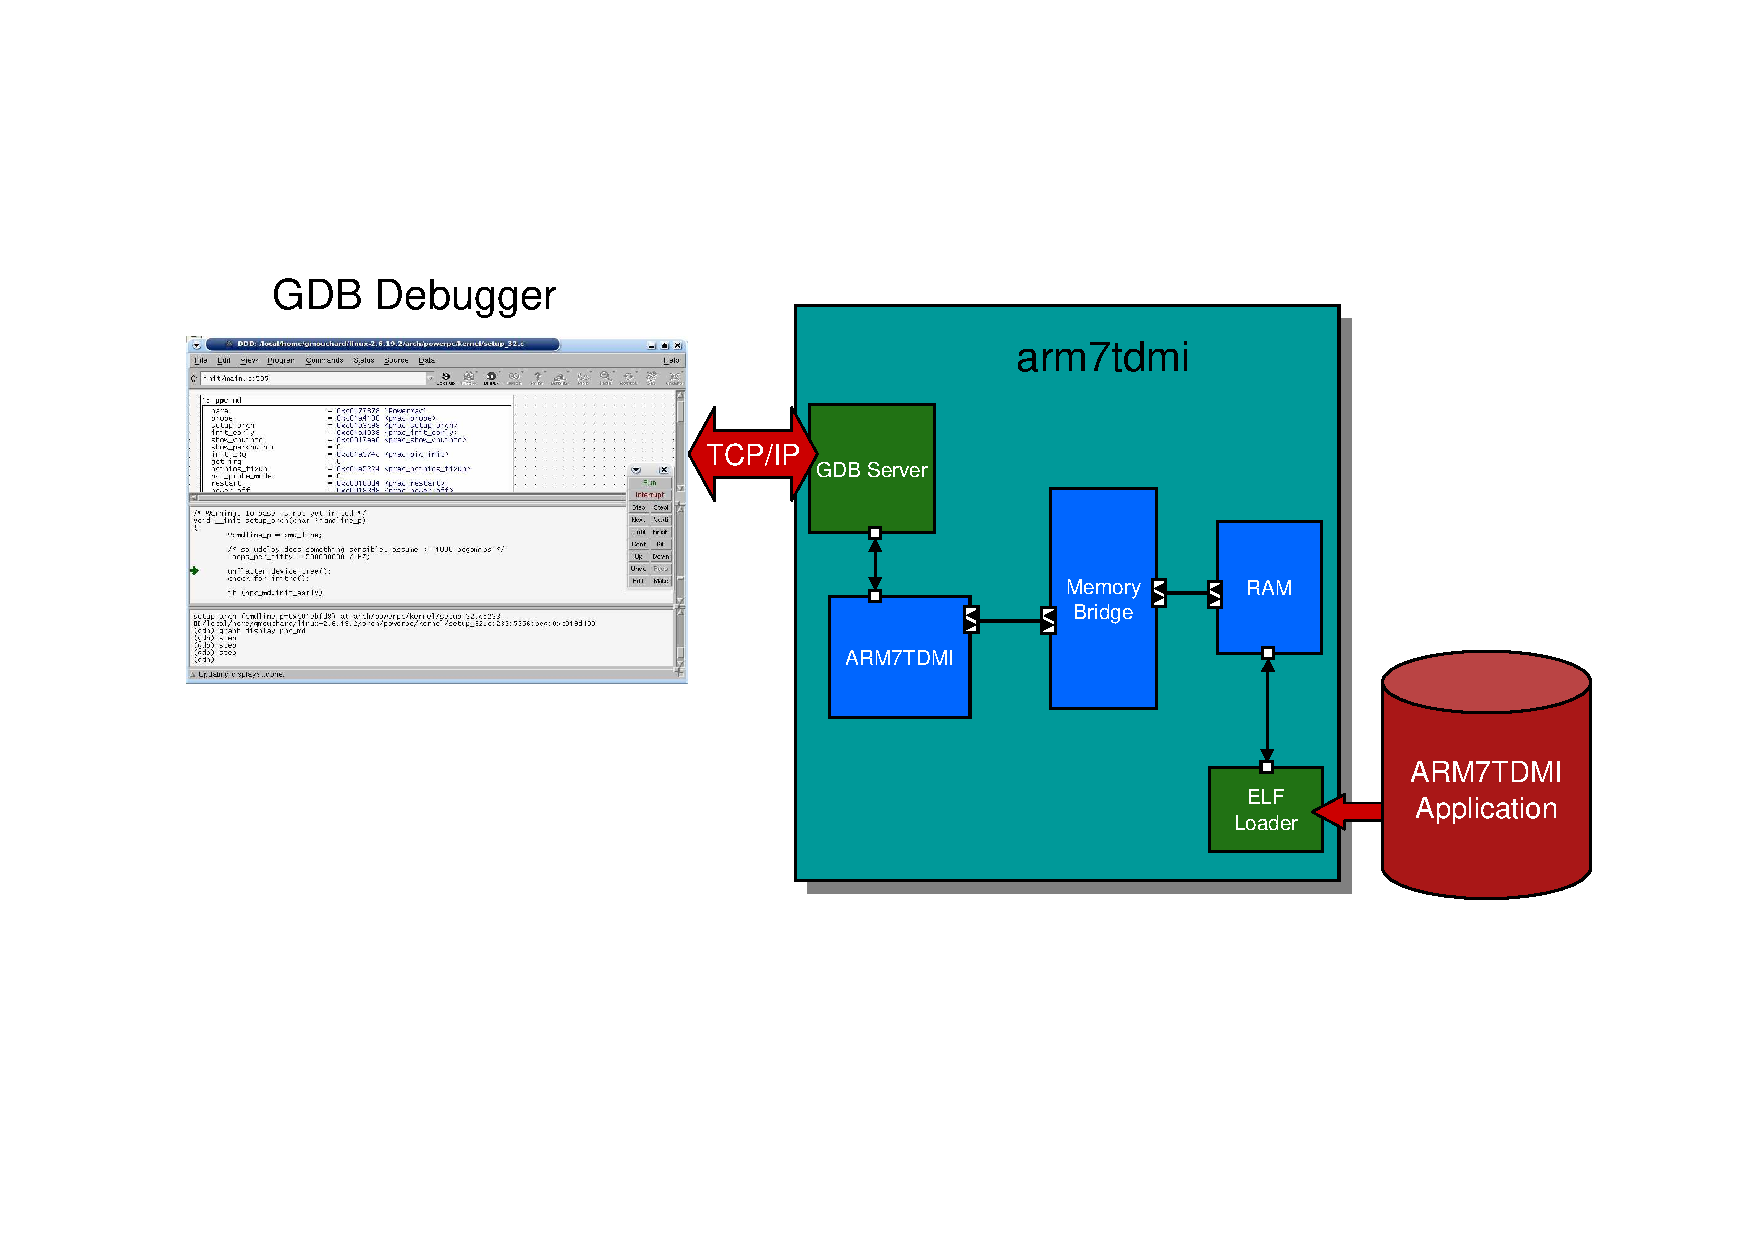
\includegraphics[width=\textwidth]{arm7tdmi/fig_arm7tdmi.pdf}
	\end{center}
	\caption{arm7tdmi simplified schematic.}
	\label{fig:arm7tdmi}
\end{figure}

Two different versions of the simulator are available:
\begin{itemize}
	\item arm7tdmi: the ARM7TDMI simulator
    \item arm7tdmi-debug: the ARM7TDMI simulator with debug information to see (traces) what is happening inside the simulator (note: it is slow)
\end{itemize}

\section{Simulated configuration}

The simulator is composed of the following modules:
\begin{itemize}\addtolength{\itemsep}{-0.40\baselineskip}
\item ARM CPU configured as an ARM7TDMI
\item Simple bus to memory bridge
\item memory
\end{itemize}

The simulator uses the following services:
\begin{itemize}\addtolength{\itemsep}{-0.40\baselineskip}
\item ELF loader
\item GDB Server
\item Inline debugger
\item SystemC Time
\item Host Time
\end{itemize}

\section{Using the simulator}

Usage: \texttt{arm7tdmi [<options>] <program> [program arguments]}

     'program' is statically linked ELF32 ARM Linux program

Options:
\begin{itemize}
\item Displaying the integrated help

\texttt{--help}
\texttt{-h}

\item Getting the simulation default configuration variables into a XML file\\
\texttt{--get-variables <xml file>}\\
\texttt{-v <xml file>}

\item Configuring the simulator with the given XML configuration file\\
\texttt{--config <xml file>}\\
\texttt{-c <xml file>}

\item Getting the simulator default configuration XML file\\
\texttt{--get-config <xml file>}\\
\texttt{-g <xml file>}\\

Note: you can use it as a template to create your own XML configuration file.

\item Activating the logger\\
\texttt{--logger}\\
\texttt{-l}

\item Defining the XML processor description file for GDB\\
\texttt{--xml-gdb <file>}\\
\texttt{-x <file>}

\item Activating the GDB server\\
\texttt{--gdb-server <port\_number>}\\
\texttt{-d <port\_number>}\\
           
Note: GDB server will use the given port\\

\item Activating the inline debugger\\
\texttt{--inline-debugger}\\
\texttt{-i}

\item Activating message spies\\
\texttt{--message-spy}\\
\texttt{-m}
\end{itemize}

The arm7tdmi simulator provides few options, but you can highly configure them using XML configuration file. To have a canvas of the XML configuration file simply run the simulator with the following option:
\begin{verbatim}
-g <xml file>
\end{verbatim}

This will generate an XML file describing the default configuration of the simulator. The following code shows you part of the initial xml configuration of the arm7tdmi:
\begin{verbatim}
<?xml version="1.0" encoding="UTF-8"?>
<VARIABLES>
  <variable>
    <type>parameter</type>
    <name>bridge.fsb-cycle-time</name>
    <data_type>unsigned long long</data_type>
    <default_value>0x0</default_value>
    <value>0x0</value>
    <description></description>
  </variable>
  <variable>
    <type>parameter</type>
    <name>bridge.mem-cycle-time</name>
    <data_type>unsigned long long</data_type>
    <default_value>0x0</default_value>
    <value>0x0</value>
    <description></description>
  </variable>
...
</VARIABLES>
\end{verbatim}

Modify the value field of the configuration parameters as you wish to set up your personal configuration, and use the -c option on the simulator to launch the simulation with your modified configuration file.


\chapter{arm966e\_s}
\label{arm966e_s}
\section{Introduction}

The arm966e\_s is a system level simulator of the ARM966E\_S processor. This simulator is a very simple simulator with just a memory connected to it. It is able to run any firmware loaded into the ram of the simulator, programs can use the full instruction set of those processors, including the Thumb instruction set. The simulator uses an elf binary loader to load into memory the firmware to simulate. Take into account that programs for those simulators require to be correctly mapped into the memory, refer to the processors manuals for more information. Software running on the simulated hardware can be debugged by connecting a GDB client to the simulator through the GDB serial remote protocol. The GDB client can be either the standard text based client (i.e. command gdb), a graphical front-end to GDB (e.g. ddd), or even Eclipse CDT. Additionally an inline debugger is also available.

The arm966e\_s does implement the CP15 coprocessor as described in the processor manual, and includes the integrated scratchpad memories (called TCM, tightly coupled memory). 

\begin{figure}[!h]
	\begin{center}
		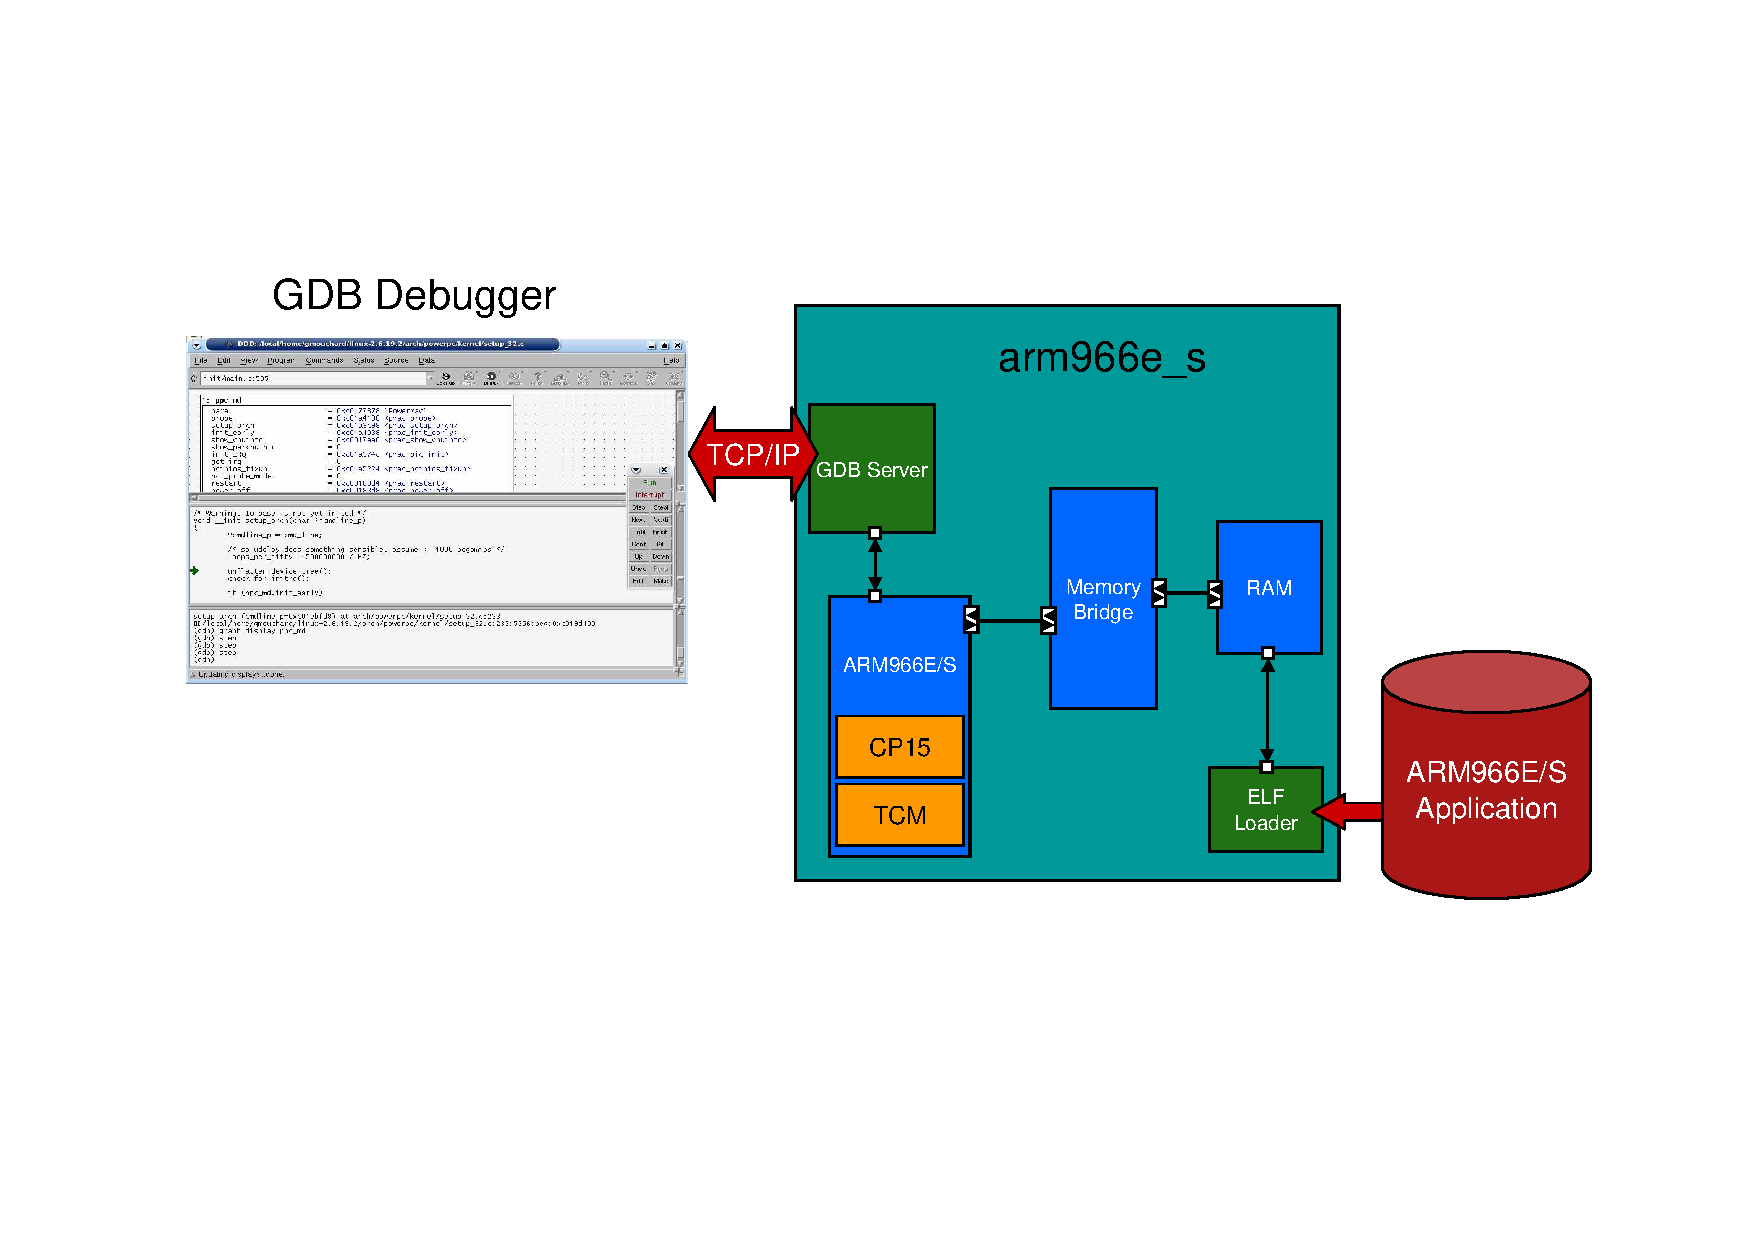
\includegraphics[width=\textwidth]{arm966e_s/fig_arm966e_s.pdf}
	\end{center}
	\caption{arm966e\_s simplified schematic.}
	\label{fig:arm966e_s}
\end{figure}

Two different versions of the simulator are available:
\begin{itemize}
	\item arm966e\_s: the ARM966E\_S simulator
    \item arm966e\_s-debug: the ARM966E\_S simulator with debug information to see (traces) what is happening inside the simulator (note: it is slow)
\end{itemize}

\section{Simulated configuration}

The simulator is composed of the following modules:
\begin{itemize}\addtolength{\itemsep}{-0.40\baselineskip}
\item ARM CPU configured as an ARM966E\_S
\item Simple bus to memory bridge
\item memory
\end{itemize}

The simulator uses the following services:
\begin{itemize}\addtolength{\itemsep}{-0.40\baselineskip}
\item ELF loader
\item GDB Server
\item Inline debugger
\item SystemC Time
\item Host Time
\end{itemize}

\section{Using the simulator}

Usage: \texttt{arm966e\_s [<options>] <program> [program arguments]}

     'program' is statically linked ELF32 ARM Linux program

Options:
\begin{itemize}
\item Displaying the integrated help

\texttt{--help}
\texttt{-h}

\item Getting the simulation default configuration variables into a XML file\\
\texttt{--get-variables <xml file>}\\
\texttt{-v <xml file>}

\item Configuring the simulator with the given XML configuration file\\
\texttt{--config <xml file>}\\
\texttt{-c <xml file>}

\item Getting the simulator default configuration XML file\\
\texttt{--get-config <xml file>}\\
\texttt{-g <xml file>}\\

Note: you can use it as a template to create your own XML configuration file.

\item Activating the logger\\
\texttt{--logger}\\
\texttt{-l}

\item Defining the XML processor description file for GDB\\
\texttt{--xml-gdb <file>}\\
\texttt{-x <file>}

\item Activating the GDB server\\
\texttt{--gdb-server <port\_number>}\\
\texttt{-d <port\_number>}\\
           
Note: GDB server will use the given port\\

\item Activating the inline debugger\\
\texttt{--inline-debugger}\\
\texttt{-i}

\item Activating message spies\\
\texttt{--message-spy}\\
\texttt{-m}
\end{itemize}

The arm966e\_s simulator provides few options, but you can highly configure them using XML configuration file. To have a canvas of the XML configuration file simply run the simulator with the following option:
\begin{verbatim}
-g <xml file>
\end{verbatim}

This will generate an XML file describing the default configuration of the simulator. The following code shows you part of the initial xml configuration of the arm966e\_s:
\begin{verbatim}
<?xml version="1.0" encoding="UTF-8"?>
<VARIABLES>
  <variable>
    <type>parameter</type>
    <name>bridge.fsb-cycle-time</name>
    <data_type>unsigned long long</data_type>
    <default_value>0x0</default_value>
    <value>0x0</value>
    <description></description>
  </variable>
  <variable>
    <type>parameter</type>
    <name>bridge.mem-cycle-time</name>
    <data_type>unsigned long long</data_type>
    <default_value>0x0</default_value>
    <value>0x0</value>
    <description></description>
  </variable>
...
</VARIABLES>
\end{verbatim}

Modify the value field of the configuration parameters as you wish to set up your personal configuration, and use the -c option on the simulator to launch the simulation with your modified configuration file.


\chapter{ppcemu}
\label{ppcemu}
This documentation has been automatically generated from the simulator \texttt{UNISIM ppcemu} version 1.0beta5 on Oct 18 2013.
\subsection{Introduction}
UNISIM ppcemu, user level PowerPC simulator with support of ELF32 binaries and Linux system call translation.\\
Section \ref{UNISIM ppcemu_licensing} gives licensing informations about the simulator.
Section \ref{UNISIM ppcemu_simulated_configuration} shows the set of modules and services that compose the simulator.
Section \ref{UNISIM ppcemu_using} shows how to invoke the simulator at the command line prompt.
Section \ref{UNISIM ppcemu_configuration} gives the simulator parameters.
Section \ref{UNISIM ppcemu_statistics} gives the simulator statistic counters.
Section \ref{UNISIM ppcemu_formulas} gives the simulator statistic formulas.
\subsection{Licensing}
\label{UNISIM ppcemu_licensing}
UNISIM ppcemu 1.0beta5\\
Copyright (C) 2007-2010, Commissariat a l'Energie Atomique (CEA)\\
License: BSD (see file COPYING)\\
Authors: Gilles Mouchard $<$gilles.mouchard@cea.fr$>$, Daniel Gracia P\'erez $<$daniel.gracia-perez@cea.fr$>$\\
\subsection{Simulated configuration}
\label{UNISIM ppcemu_simulated_configuration}
\begin{figure}[!ht]
	\begin{center}
		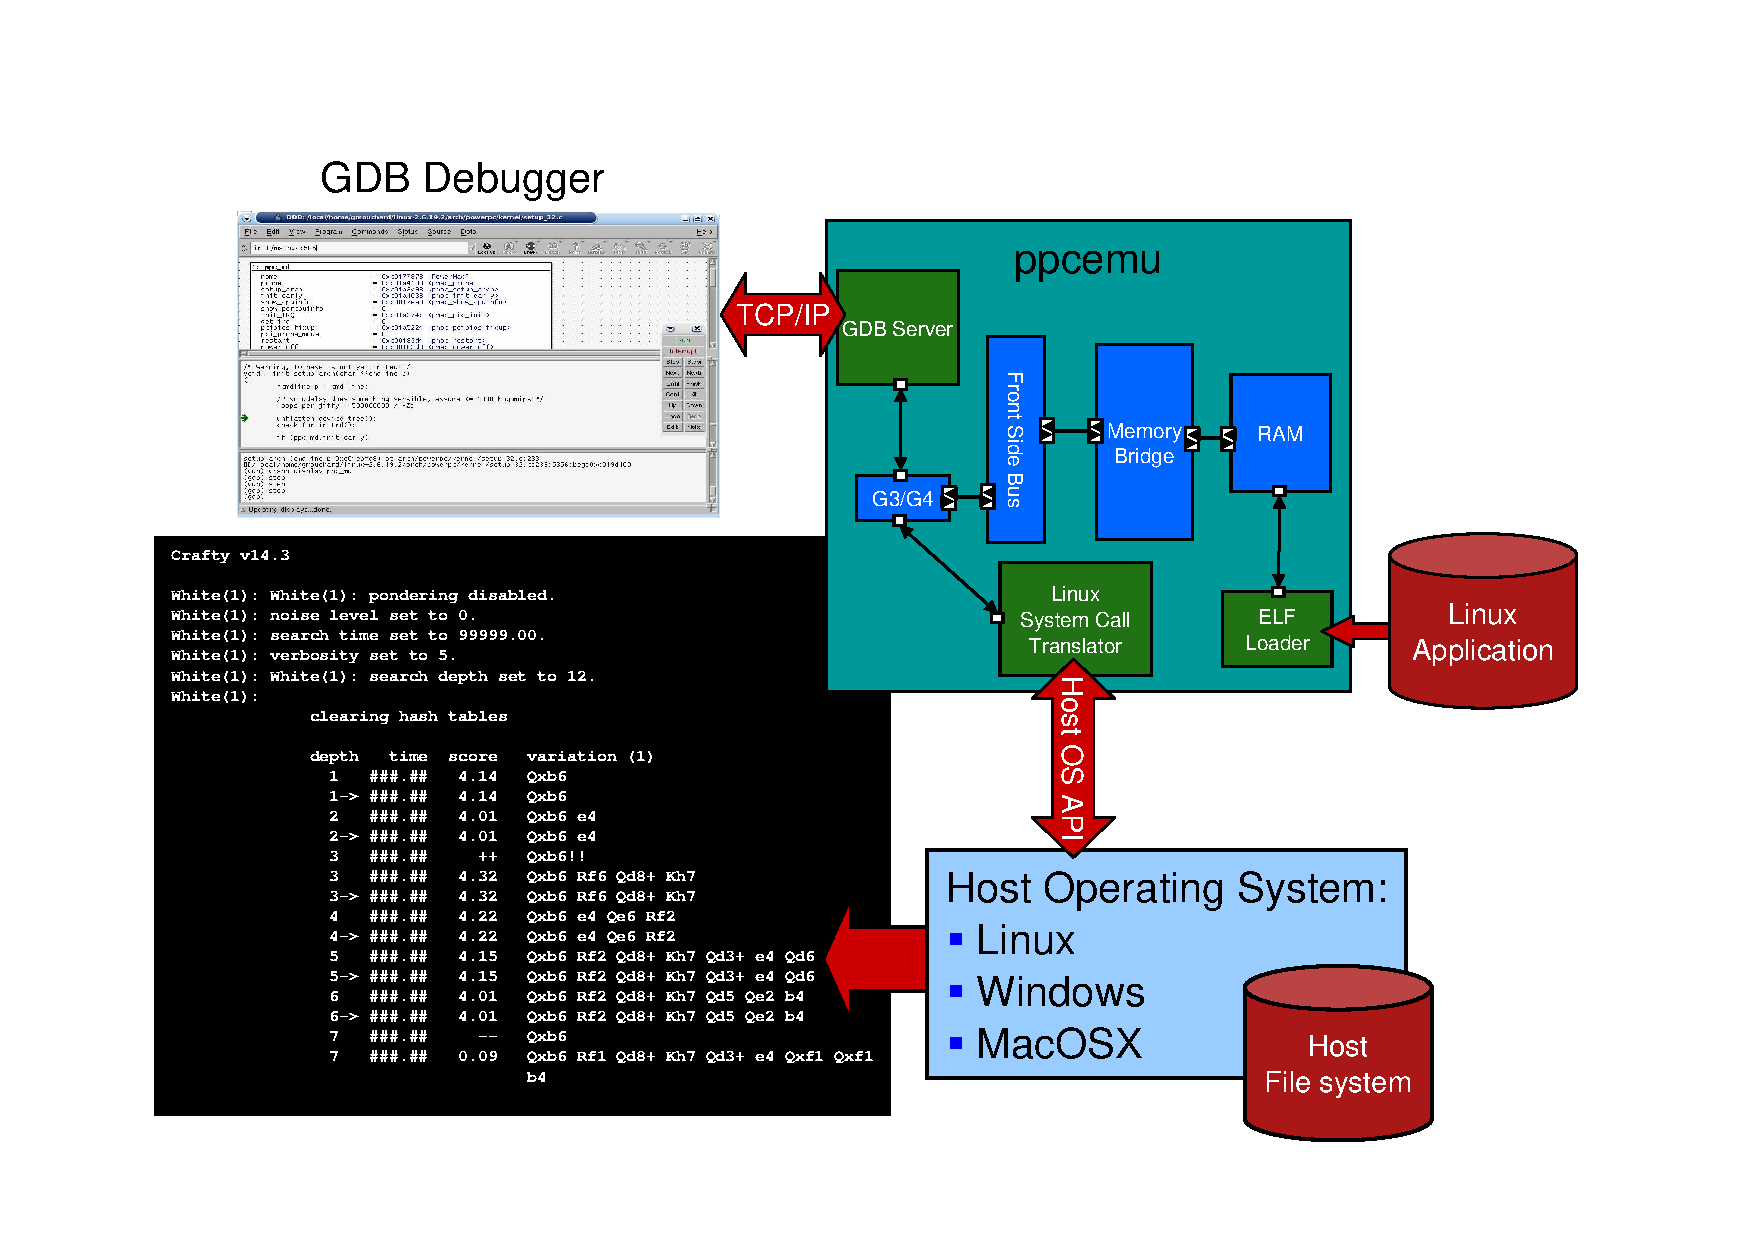
\includegraphics[width=\textwidth]{ppcemu/fig_schematic.pdf}
	\end{center}
	\caption{UNISIM ppcemu simulator schematic.}
\end{figure}
\noindent The UNISIM ppcemu simulator is composed of the following modules and services:
\begin{itemize}\addtolength{\itemsep}{-0.40\baselineskip}
\item \textbf{cpu}: this module implements a MPC7447A CPU core
\item \textbf{debugger}
\item \textbf{gdb-server}: this service implements the GDB server remote serial protocol over TCP/IP. Standards GDB clients (e.g. gdb, eclipse, ddd) can connect to the simulator to debug the target application that runs within the simulator.
\item \textbf{host-time}: this service is an abstraction layer for the host machine time
\item \textbf{inline-debugger}: this service implements a built-in debugger in the terminal console
\item \textbf{linux-os}
\item \textbf{memory}: this module implements a memory
\item \textbf{profiler}
\item \textbf{tee-memory-access-reporting}
\item \textbf{tee-memory-access-reporting.tee-memory-access-reporting.control\_selector[0]}
\item \textbf{tee-memory-access-reporting.tee-memory-access-reporting.control\_selector[10]}
\item \textbf{tee-memory-access-reporting.tee-memory-access-reporting.control\_selector[11]}
\item \textbf{tee-memory-access-reporting.tee-memory-access-reporting.control\_selector[12]}
\item \textbf{tee-memory-access-reporting.tee-memory-access-reporting.control\_selector[13]}
\item \textbf{tee-memory-access-reporting.tee-memory-access-reporting.control\_selector[14]}
\item \textbf{tee-memory-access-reporting.tee-memory-access-reporting.control\_selector[15]}
\item \textbf{tee-memory-access-reporting.tee-memory-access-reporting.control\_selector[1]}
\item \textbf{tee-memory-access-reporting.tee-memory-access-reporting.control\_selector[2]}
\item \textbf{tee-memory-access-reporting.tee-memory-access-reporting.control\_selector[3]}
\item \textbf{tee-memory-access-reporting.tee-memory-access-reporting.control\_selector[4]}
\item \textbf{tee-memory-access-reporting.tee-memory-access-reporting.control\_selector[5]}
\item \textbf{tee-memory-access-reporting.tee-memory-access-reporting.control\_selector[6]}
\item \textbf{tee-memory-access-reporting.tee-memory-access-reporting.control\_selector[7]}
\item \textbf{tee-memory-access-reporting.tee-memory-access-reporting.control\_selector[8]}
\item \textbf{tee-memory-access-reporting.tee-memory-access-reporting.control\_selector[9]}
\item \textbf{time}: this service is an abstraction layer for the SystemC kernel time
\end{itemize}
\subsection{Using the UNISIM ppcemu simulator}
\label{UNISIM ppcemu_using}
The UNISIM ppcemu simulator has the following command line options:\\
~\\
\noindent Usage: \texttt{unisim-ppcemu-1.0beta5 [<options>] [...]}

\noindent Options:
\begin{itemize}
\item \texttt{--set $<$param=value$>$ or -s $<$param=value$>$}: set value of parameter 'param' to 'value'
\item \texttt{--config $<$XML file$>$ or -c $<$XML file$>$}: configures the simulator with the given XML configuration file
\item \texttt{--get-config $<$XML file$>$ or -g $<$XML file$>$}: get the simulator configuration XML file (you can use it to create your own configuration. This option can be combined with -c to get a new configuration file with existing variables from another file
\item \texttt{--list or -l}: lists all available parameters, their type, and their current value
\item \texttt{--warn or -w}: enable printing of kernel warnings
\item \texttt{--doc $<$Latex file$>$ or -d $<$Latex file$>$}: enable printing a latex documentation
\item \texttt{--version or -v}: displays the program version information
\item \texttt{--share-path $<$path$>$ or -p $<$path$>$}: the path that should be used for the share directory (absolute path)
\item \texttt{--help or -h}: displays this help
\end{itemize}
\subsection{Configuration}
\label{UNISIM ppcemu_configuration}
Simulator configuration (see below) can be modified using command line Options \texttt{--set $<$param=value$>$} or \texttt{--config $<$config file$>$}.\\
~\\
\tablehead{\hline}
\tabletail{\hline}
\begin{supertabular}{|p{7.5cm}|p{7.5cm}|}
\multicolumn{2}{|l|}{\textbf{\Large Global}}\\
\hline
\multicolumn{1}{|p{7.5cm}}{\textbf{Name:} \texttt{enable-gdb-server}} & \multicolumn{1}{p{7.5cm}|}{\textbf{Type:} \texttt{parameter}}\\
\multicolumn{1}{|p{7.5cm}}{\textbf{Default:} \texttt{true}} & \multicolumn{1}{p{7.5cm}|}{\textbf{Data type:} \texttt{boolean}}\\
\multicolumn{2}{|p{15cm}|}{\textbf{Valid:} \texttt{true},~\texttt{false}}\\
\multicolumn{2}{|l|}{}\\
\multicolumn{2}{|p{15cm}|}{\textbf{Description:} \newline Enable/Disable GDB server instantiation.}\\
\hline
\multicolumn{1}{|p{7.5cm}}{\textbf{Name:} \texttt{enable-inline-debugger}} & \multicolumn{1}{p{7.5cm}|}{\textbf{Type:} \texttt{parameter}}\\
\multicolumn{1}{|p{7.5cm}}{\textbf{Default:} \texttt{true}} & \multicolumn{1}{p{7.5cm}|}{\textbf{Data type:} \texttt{boolean}}\\
\multicolumn{2}{|p{15cm}|}{\textbf{Valid:} \texttt{true},~\texttt{false}}\\
\multicolumn{2}{|l|}{}\\
\multicolumn{2}{|p{15cm}|}{\textbf{Description:} \newline Enable/Disable inline debugger instantiation.}\\
\hline
\multicolumn{1}{|p{7.5cm}}{\textbf{Name:} \texttt{enable-press-enter-at-exit}} & \multicolumn{1}{p{7.5cm}|}{\textbf{Type:} \texttt{parameter}}\\
\multicolumn{1}{|p{7.5cm}}{\textbf{Default:} \texttt{false}} & \multicolumn{1}{p{7.5cm}|}{\textbf{Data type:} \texttt{boolean}}\\
\multicolumn{2}{|p{15cm}|}{\textbf{Valid:} \texttt{true},~\texttt{false}}\\
\multicolumn{2}{|l|}{}\\
\multicolumn{2}{|p{15cm}|}{\textbf{Description:} \newline Enable/Disable pressing key enter at exit.}\\
\hline
\multicolumn{1}{|p{7.5cm}}{\textbf{Name:} \texttt{estimate-power}} & \multicolumn{1}{p{7.5cm}|}{\textbf{Type:} \texttt{parameter}}\\
\multicolumn{1}{|p{7.5cm}}{\textbf{Default:} \texttt{false}} & \multicolumn{1}{p{7.5cm}|}{\textbf{Data type:} \texttt{boolean}}\\
\multicolumn{2}{|p{15cm}|}{\textbf{Valid:} \texttt{true},~\texttt{false}}\\
\multicolumn{2}{|l|}{}\\
\multicolumn{2}{|p{15cm}|}{\textbf{Description:} \newline Enable/Disable power estimators instantiation.}\\
\hline
\multicolumn{1}{|p{7.5cm}}{\textbf{Name:} \texttt{kernel\_logger.file}} & \multicolumn{1}{p{7.5cm}|}{\textbf{Type:} \texttt{parameter}}\\
\multicolumn{1}{|p{7.5cm}}{\textbf{Default:} \texttt{false}} & \multicolumn{1}{p{7.5cm}|}{\textbf{Data type:} \texttt{boolean}}\\
\multicolumn{2}{|p{15cm}|}{\textbf{Valid:} \texttt{true},~\texttt{false}}\\
\multicolumn{2}{|l|}{}\\
\multicolumn{2}{|p{15cm}|}{\textbf{Description:} \newline Keep logger output in a file.}\\
\hline
\multicolumn{1}{|p{7.5cm}}{\textbf{Name:} \texttt{kernel\_logger.filename}} & \multicolumn{1}{p{7.5cm}|}{\textbf{Type:} \texttt{parameter}}\\
\multicolumn{1}{|p{7.5cm}}{\textbf{Default:} \texttt{logger\_output.txt}} & \multicolumn{1}{p{7.5cm}|}{\textbf{Data type:} \texttt{string}}\\
\multicolumn{2}{|l|}{}\\
\multicolumn{2}{|l|}{}\\
\multicolumn{2}{|p{15cm}|}{\textbf{Description:} \newline Filename to keep logger output \_(the option file must be activated).}\\
\hline
\multicolumn{1}{|p{7.5cm}}{\textbf{Name:} \texttt{kernel\_logger.std\_err}} & \multicolumn{1}{p{7.5cm}|}{\textbf{Type:} \texttt{parameter}}\\
\multicolumn{1}{|p{7.5cm}}{\textbf{Default:} \texttt{true}} & \multicolumn{1}{p{7.5cm}|}{\textbf{Data type:} \texttt{boolean}}\\
\multicolumn{2}{|p{15cm}|}{\textbf{Valid:} \texttt{true},~\texttt{false}}\\
\multicolumn{2}{|l|}{}\\
\multicolumn{2}{|p{15cm}|}{\textbf{Description:} \newline Show logger output through the standard error output.}\\
\hline
\multicolumn{1}{|p{7.5cm}}{\textbf{Name:} \texttt{kernel\_logger.std\_err\_color}} & \multicolumn{1}{p{7.5cm}|}{\textbf{Type:} \texttt{parameter}}\\
\multicolumn{1}{|p{7.5cm}}{\textbf{Default:} \texttt{false}} & \multicolumn{1}{p{7.5cm}|}{\textbf{Data type:} \texttt{boolean}}\\
\multicolumn{2}{|p{15cm}|}{\textbf{Valid:} \texttt{true},~\texttt{false}}\\
\multicolumn{2}{|l|}{}\\
\multicolumn{2}{|p{15cm}|}{\textbf{Description:} \newline Colorize logger output through the standard error output \_(only works if std\_err is active).}\\
\hline
\multicolumn{1}{|p{7.5cm}}{\textbf{Name:} \texttt{kernel\_logger.std\_out}} & \multicolumn{1}{p{7.5cm}|}{\textbf{Type:} \texttt{parameter}}\\
\multicolumn{1}{|p{7.5cm}}{\textbf{Default:} \texttt{false}} & \multicolumn{1}{p{7.5cm}|}{\textbf{Data type:} \texttt{boolean}}\\
\multicolumn{2}{|p{15cm}|}{\textbf{Valid:} \texttt{true},~\texttt{false}}\\
\multicolumn{2}{|l|}{}\\
\multicolumn{2}{|p{15cm}|}{\textbf{Description:} \newline Show logger output through the standard output.}\\
\hline
\multicolumn{1}{|p{7.5cm}}{\textbf{Name:} \texttt{kernel\_logger.std\_out\_color}} & \multicolumn{1}{p{7.5cm}|}{\textbf{Type:} \texttt{parameter}}\\
\multicolumn{1}{|p{7.5cm}}{\textbf{Default:} \texttt{false}} & \multicolumn{1}{p{7.5cm}|}{\textbf{Data type:} \texttt{boolean}}\\
\multicolumn{2}{|p{15cm}|}{\textbf{Valid:} \texttt{true},~\texttt{false}}\\
\multicolumn{2}{|l|}{}\\
\multicolumn{2}{|p{15cm}|}{\textbf{Description:} \newline Colorize logger output through the standard output \_(only works if std\_out is active).}\\
\hline
\multicolumn{1}{|p{7.5cm}}{\textbf{Name:} \texttt{kernel\_logger.xml\_file}} & \multicolumn{1}{p{7.5cm}|}{\textbf{Type:} \texttt{parameter}}\\
\multicolumn{1}{|p{7.5cm}}{\textbf{Default:} \texttt{false}} & \multicolumn{1}{p{7.5cm}|}{\textbf{Data type:} \texttt{boolean}}\\
\multicolumn{2}{|p{15cm}|}{\textbf{Valid:} \texttt{true},~\texttt{false}}\\
\multicolumn{2}{|l|}{}\\
\multicolumn{2}{|p{15cm}|}{\textbf{Description:} \newline Keep logger output in a file xml formatted.}\\
\hline
\multicolumn{1}{|p{7.5cm}}{\textbf{Name:} \texttt{kernel\_logger.xml\_file\_gzipped}} & \multicolumn{1}{p{7.5cm}|}{\textbf{Type:} \texttt{parameter}}\\
\multicolumn{1}{|p{7.5cm}}{\textbf{Default:} \texttt{false}} & \multicolumn{1}{p{7.5cm}|}{\textbf{Data type:} \texttt{boolean}}\\
\multicolumn{2}{|p{15cm}|}{\textbf{Valid:} \texttt{true},~\texttt{false}}\\
\multicolumn{2}{|l|}{}\\
\multicolumn{2}{|p{15cm}|}{\textbf{Description:} \newline If the xml\_file option is active, the output file will be compressed (a .gz extension will be automatically added to the xml\_filename option.}\\
\hline
\multicolumn{1}{|p{7.5cm}}{\textbf{Name:} \texttt{kernel\_logger.xml\_filename}} & \multicolumn{1}{p{7.5cm}|}{\textbf{Type:} \texttt{parameter}}\\
\multicolumn{1}{|p{7.5cm}}{\textbf{Default:} \texttt{logger\_output.xml}} & \multicolumn{1}{p{7.5cm}|}{\textbf{Data type:} \texttt{string}}\\
\multicolumn{2}{|l|}{}\\
\multicolumn{2}{|l|}{}\\
\multicolumn{2}{|p{15cm}|}{\textbf{Description:} \newline Filename to keep logger xml output \_(the option xml\_file must be activated).}\\
\hline
\hline
\multicolumn{2}{|l|}{\textbf{\Large cpu}}\\
\hline
\multicolumn{1}{|p{7.5cm}}{\textbf{Name:} \texttt{cpu.cpu-cycle-time}} & \multicolumn{1}{p{7.5cm}|}{\textbf{Type:} \texttt{parameter}}\\
\multicolumn{1}{|p{7.5cm}}{\textbf{Default:} \texttt{3333}} & \multicolumn{1}{p{7.5cm}|}{\textbf{Data type:} \texttt{unsigned 64-bit integer}}\\
\multicolumn{2}{|l|}{}\\
\multicolumn{2}{|l|}{}\\
\multicolumn{2}{|p{15cm}|}{\textbf{Description:} \newline CPU cycle time in picoseconds.}\\
\hline
\multicolumn{1}{|p{7.5cm}}{\textbf{Name:} \texttt{cpu.voltage}} & \multicolumn{1}{p{7.5cm}|}{\textbf{Type:} \texttt{parameter}}\\
\multicolumn{1}{|p{7.5cm}}{\textbf{Default:} \texttt{1300}} & \multicolumn{1}{p{7.5cm}|}{\textbf{Data type:} \texttt{unsigned 64-bit integer}}\\
\multicolumn{2}{|l|}{}\\
\multicolumn{2}{|l|}{}\\
\multicolumn{2}{|p{15cm}|}{\textbf{Description:} \newline CPU voltage in mV.}\\
\hline
\multicolumn{1}{|p{7.5cm}}{\textbf{Name:} \texttt{cpu.max-inst}} & \multicolumn{1}{p{7.5cm}|}{\textbf{Type:} \texttt{parameter}}\\
\multicolumn{1}{|p{7.5cm}}{\textbf{Default:} \texttt{18446744073709551615}} & \multicolumn{1}{p{7.5cm}|}{\textbf{Data type:} \texttt{unsigned 64-bit integer}}\\
\multicolumn{2}{|l|}{}\\
\multicolumn{2}{|l|}{}\\
\multicolumn{2}{|p{15cm}|}{\textbf{Description:} \newline maximum number of instructions to simulate.}\\
\hline
\multicolumn{1}{|p{7.5cm}}{\textbf{Name:} \texttt{cpu.verbose-all}} & \multicolumn{1}{p{7.5cm}|}{\textbf{Type:} \texttt{parameter}}\\
\multicolumn{1}{|p{7.5cm}}{\textbf{Default:} \texttt{false}} & \multicolumn{1}{p{7.5cm}|}{\textbf{Data type:} \texttt{boolean}}\\
\multicolumn{2}{|p{15cm}|}{\textbf{Valid:} \texttt{true},~\texttt{false}}\\
\multicolumn{2}{|l|}{}\\
\multicolumn{2}{|p{15cm}|}{\textbf{Description:} \newline globally enable/disable verbosity.}\\
\hline
\multicolumn{1}{|p{7.5cm}}{\textbf{Name:} \texttt{cpu.verbose-setup}} & \multicolumn{1}{p{7.5cm}|}{\textbf{Type:} \texttt{parameter}}\\
\multicolumn{1}{|p{7.5cm}}{\textbf{Default:} \texttt{false}} & \multicolumn{1}{p{7.5cm}|}{\textbf{Data type:} \texttt{boolean}}\\
\multicolumn{2}{|p{15cm}|}{\textbf{Valid:} \texttt{true},~\texttt{false}}\\
\multicolumn{2}{|l|}{}\\
\multicolumn{2}{|p{15cm}|}{\textbf{Description:} \newline enable/disable verbosity while setup.}\\
\hline
\multicolumn{1}{|p{7.5cm}}{\textbf{Name:} \texttt{cpu.verbose-step}} & \multicolumn{1}{p{7.5cm}|}{\textbf{Type:} \texttt{parameter}}\\
\multicolumn{1}{|p{7.5cm}}{\textbf{Default:} \texttt{false}} & \multicolumn{1}{p{7.5cm}|}{\textbf{Data type:} \texttt{boolean}}\\
\multicolumn{2}{|p{15cm}|}{\textbf{Valid:} \texttt{true},~\texttt{false}}\\
\multicolumn{2}{|l|}{}\\
\multicolumn{2}{|p{15cm}|}{\textbf{Description:} \newline enable/disable verbosity when simulating an instruction.}\\
\hline
\multicolumn{1}{|p{7.5cm}}{\textbf{Name:} \texttt{cpu.verbose-dtlb}} & \multicolumn{1}{p{7.5cm}|}{\textbf{Type:} \texttt{parameter}}\\
\multicolumn{1}{|p{7.5cm}}{\textbf{Default:} \texttt{false}} & \multicolumn{1}{p{7.5cm}|}{\textbf{Data type:} \texttt{boolean}}\\
\multicolumn{2}{|p{15cm}|}{\textbf{Valid:} \texttt{true},~\texttt{false}}\\
\multicolumn{2}{|l|}{}\\
\multicolumn{2}{|p{15cm}|}{\textbf{Description:} \newline enable/disable verbosity when accessing data translation lookahead buffer.}\\
\hline
\multicolumn{1}{|p{7.5cm}}{\textbf{Name:} \texttt{cpu.verbose-itlb}} & \multicolumn{1}{p{7.5cm}|}{\textbf{Type:} \texttt{parameter}}\\
\multicolumn{1}{|p{7.5cm}}{\textbf{Default:} \texttt{false}} & \multicolumn{1}{p{7.5cm}|}{\textbf{Data type:} \texttt{boolean}}\\
\multicolumn{2}{|p{15cm}|}{\textbf{Valid:} \texttt{true},~\texttt{false}}\\
\multicolumn{2}{|l|}{}\\
\multicolumn{2}{|p{15cm}|}{\textbf{Description:} \newline enable/disable verbosity when accessing instruction translation lookahead buffer.}\\
\hline
\multicolumn{1}{|p{7.5cm}}{\textbf{Name:} \texttt{cpu.verbose-dl1}} & \multicolumn{1}{p{7.5cm}|}{\textbf{Type:} \texttt{parameter}}\\
\multicolumn{1}{|p{7.5cm}}{\textbf{Default:} \texttt{false}} & \multicolumn{1}{p{7.5cm}|}{\textbf{Data type:} \texttt{boolean}}\\
\multicolumn{2}{|p{15cm}|}{\textbf{Valid:} \texttt{true},~\texttt{false}}\\
\multicolumn{2}{|l|}{}\\
\multicolumn{2}{|p{15cm}|}{\textbf{Description:} \newline enable/disable verbosity when accessing L1 data cache.}\\
\hline
\multicolumn{1}{|p{7.5cm}}{\textbf{Name:} \texttt{cpu.verbose-il1}} & \multicolumn{1}{p{7.5cm}|}{\textbf{Type:} \texttt{parameter}}\\
\multicolumn{1}{|p{7.5cm}}{\textbf{Default:} \texttt{false}} & \multicolumn{1}{p{7.5cm}|}{\textbf{Data type:} \texttt{boolean}}\\
\multicolumn{2}{|p{15cm}|}{\textbf{Valid:} \texttt{true},~\texttt{false}}\\
\multicolumn{2}{|l|}{}\\
\multicolumn{2}{|p{15cm}|}{\textbf{Description:} \newline enable/disable verbosity when accessing L1 instruction cache.}\\
\hline
\multicolumn{1}{|p{7.5cm}}{\textbf{Name:} \texttt{cpu.verbose-l2}} & \multicolumn{1}{p{7.5cm}|}{\textbf{Type:} \texttt{parameter}}\\
\multicolumn{1}{|p{7.5cm}}{\textbf{Default:} \texttt{false}} & \multicolumn{1}{p{7.5cm}|}{\textbf{Data type:} \texttt{boolean}}\\
\multicolumn{2}{|p{15cm}|}{\textbf{Valid:} \texttt{true},~\texttt{false}}\\
\multicolumn{2}{|l|}{}\\
\multicolumn{2}{|p{15cm}|}{\textbf{Description:} \newline enable/disable verbosity when accessing L2 unified cache.}\\
\hline
\multicolumn{1}{|p{7.5cm}}{\textbf{Name:} \texttt{cpu.verbose-load}} & \multicolumn{1}{p{7.5cm}|}{\textbf{Type:} \texttt{parameter}}\\
\multicolumn{1}{|p{7.5cm}}{\textbf{Default:} \texttt{false}} & \multicolumn{1}{p{7.5cm}|}{\textbf{Data type:} \texttt{boolean}}\\
\multicolumn{2}{|p{15cm}|}{\textbf{Valid:} \texttt{true},~\texttt{false}}\\
\multicolumn{2}{|l|}{}\\
\multicolumn{2}{|p{15cm}|}{\textbf{Description:} \newline enable/disable verbosity when simulating a load.}\\
\hline
\multicolumn{1}{|p{7.5cm}}{\textbf{Name:} \texttt{cpu.verbose-store}} & \multicolumn{1}{p{7.5cm}|}{\textbf{Type:} \texttt{parameter}}\\
\multicolumn{1}{|p{7.5cm}}{\textbf{Default:} \texttt{false}} & \multicolumn{1}{p{7.5cm}|}{\textbf{Data type:} \texttt{boolean}}\\
\multicolumn{2}{|p{15cm}|}{\textbf{Valid:} \texttt{true},~\texttt{false}}\\
\multicolumn{2}{|l|}{}\\
\multicolumn{2}{|p{15cm}|}{\textbf{Description:} \newline enable/disable verbosity when simulating a store.}\\
\hline
\multicolumn{1}{|p{7.5cm}}{\textbf{Name:} \texttt{cpu.verbose-read-memory}} & \multicolumn{1}{p{7.5cm}|}{\textbf{Type:} \texttt{parameter}}\\
\multicolumn{1}{|p{7.5cm}}{\textbf{Default:} \texttt{false}} & \multicolumn{1}{p{7.5cm}|}{\textbf{Data type:} \texttt{boolean}}\\
\multicolumn{2}{|p{15cm}|}{\textbf{Valid:} \texttt{true},~\texttt{false}}\\
\multicolumn{2}{|l|}{}\\
\multicolumn{2}{|p{15cm}|}{\textbf{Description:} \newline enable/disable verbosity when reading memory for a debug purpose.}\\
\hline
\multicolumn{1}{|p{7.5cm}}{\textbf{Name:} \texttt{cpu.verbose-write-memory}} & \multicolumn{1}{p{7.5cm}|}{\textbf{Type:} \texttt{parameter}}\\
\multicolumn{1}{|p{7.5cm}}{\textbf{Default:} \texttt{false}} & \multicolumn{1}{p{7.5cm}|}{\textbf{Data type:} \texttt{boolean}}\\
\multicolumn{2}{|p{15cm}|}{\textbf{Valid:} \texttt{true},~\texttt{false}}\\
\multicolumn{2}{|l|}{}\\
\multicolumn{2}{|p{15cm}|}{\textbf{Description:} \newline enable/disable verbosity when writing memory for a debug purpose.}\\
\hline
\multicolumn{1}{|p{7.5cm}}{\textbf{Name:} \texttt{cpu.verbose-exception}} & \multicolumn{1}{p{7.5cm}|}{\textbf{Type:} \texttt{parameter}}\\
\multicolumn{1}{|p{7.5cm}}{\textbf{Default:} \texttt{false}} & \multicolumn{1}{p{7.5cm}|}{\textbf{Data type:} \texttt{boolean}}\\
\multicolumn{2}{|p{15cm}|}{\textbf{Valid:} \texttt{true},~\texttt{false}}\\
\multicolumn{2}{|l|}{}\\
\multicolumn{2}{|p{15cm}|}{\textbf{Description:} \newline enable/disable verbosity when handling exceptions.}\\
\hline
\multicolumn{1}{|p{7.5cm}}{\textbf{Name:} \texttt{cpu.verbose-set-msr}} & \multicolumn{1}{p{7.5cm}|}{\textbf{Type:} \texttt{parameter}}\\
\multicolumn{1}{|p{7.5cm}}{\textbf{Default:} \texttt{false}} & \multicolumn{1}{p{7.5cm}|}{\textbf{Data type:} \texttt{boolean}}\\
\multicolumn{2}{|p{15cm}|}{\textbf{Valid:} \texttt{true},~\texttt{false}}\\
\multicolumn{2}{|l|}{}\\
\multicolumn{2}{|p{15cm}|}{\textbf{Description:} \newline enable/disable verbosity when setting MSR.}\\
\hline
\multicolumn{1}{|p{7.5cm}}{\textbf{Name:} \texttt{cpu.verbose-set-hid0}} & \multicolumn{1}{p{7.5cm}|}{\textbf{Type:} \texttt{parameter}}\\
\multicolumn{1}{|p{7.5cm}}{\textbf{Default:} \texttt{false}} & \multicolumn{1}{p{7.5cm}|}{\textbf{Data type:} \texttt{boolean}}\\
\multicolumn{2}{|p{15cm}|}{\textbf{Valid:} \texttt{true},~\texttt{false}}\\
\multicolumn{2}{|l|}{}\\
\multicolumn{2}{|p{15cm}|}{\textbf{Description:} \newline enable/disable verbosity when setting HID0.}\\
\hline
\multicolumn{1}{|p{7.5cm}}{\textbf{Name:} \texttt{cpu.verbose-set-hid1}} & \multicolumn{1}{p{7.5cm}|}{\textbf{Type:} \texttt{parameter}}\\
\multicolumn{1}{|p{7.5cm}}{\textbf{Default:} \texttt{false}} & \multicolumn{1}{p{7.5cm}|}{\textbf{Data type:} \texttt{boolean}}\\
\multicolumn{2}{|p{15cm}|}{\textbf{Valid:} \texttt{true},~\texttt{false}}\\
\multicolumn{2}{|l|}{}\\
\multicolumn{2}{|p{15cm}|}{\textbf{Description:} \newline enable/disable verbosity when setting HID1.}\\
\hline
\multicolumn{1}{|p{7.5cm}}{\textbf{Name:} \texttt{cpu.verbose-set-hid2}} & \multicolumn{1}{p{7.5cm}|}{\textbf{Type:} \texttt{parameter}}\\
\multicolumn{1}{|p{7.5cm}}{\textbf{Default:} \texttt{false}} & \multicolumn{1}{p{7.5cm}|}{\textbf{Data type:} \texttt{boolean}}\\
\multicolumn{2}{|p{15cm}|}{\textbf{Valid:} \texttt{true},~\texttt{false}}\\
\multicolumn{2}{|l|}{}\\
\multicolumn{2}{|p{15cm}|}{\textbf{Description:} \newline enable/disable verbosity when setting HID2.}\\
\hline
\multicolumn{1}{|p{7.5cm}}{\textbf{Name:} \texttt{cpu.verbose-set-l2cr}} & \multicolumn{1}{p{7.5cm}|}{\textbf{Type:} \texttt{parameter}}\\
\multicolumn{1}{|p{7.5cm}}{\textbf{Default:} \texttt{false}} & \multicolumn{1}{p{7.5cm}|}{\textbf{Data type:} \texttt{boolean}}\\
\multicolumn{2}{|p{15cm}|}{\textbf{Valid:} \texttt{true},~\texttt{false}}\\
\multicolumn{2}{|l|}{}\\
\multicolumn{2}{|p{15cm}|}{\textbf{Description:} \newline enable/disable verbosity when setting L2CR.}\\
\hline
\multicolumn{1}{|p{7.5cm}}{\textbf{Name:} \texttt{cpu.enable-linux-printk-snooping}} & \multicolumn{1}{p{7.5cm}|}{\textbf{Type:} \texttt{parameter}}\\
\multicolumn{1}{|p{7.5cm}}{\textbf{Default:} \texttt{false}} & \multicolumn{1}{p{7.5cm}|}{\textbf{Data type:} \texttt{boolean}}\\
\multicolumn{2}{|p{15cm}|}{\textbf{Valid:} \texttt{true},~\texttt{false}}\\
\multicolumn{2}{|l|}{}\\
\multicolumn{2}{|p{15cm}|}{\textbf{Description:} \newline enable/disable linux printk buffer snooping.}\\
\hline
\multicolumn{1}{|p{7.5cm}}{\textbf{Name:} \texttt{cpu.enable-linux-syscall-snooping}} & \multicolumn{1}{p{7.5cm}|}{\textbf{Type:} \texttt{parameter}}\\
\multicolumn{1}{|p{7.5cm}}{\textbf{Default:} \texttt{false}} & \multicolumn{1}{p{7.5cm}|}{\textbf{Data type:} \texttt{boolean}}\\
\multicolumn{2}{|p{15cm}|}{\textbf{Valid:} \texttt{true},~\texttt{false}}\\
\multicolumn{2}{|l|}{}\\
\multicolumn{2}{|p{15cm}|}{\textbf{Description:} \newline enable/disable linux syscall snooping.}\\
\hline
\multicolumn{1}{|p{7.5cm}}{\textbf{Name:} \texttt{cpu.trap-on-instruction-counter}} & \multicolumn{1}{p{7.5cm}|}{\textbf{Type:} \texttt{parameter}}\\
\multicolumn{1}{|p{7.5cm}}{\textbf{Default:} \texttt{18446744073709551615}} & \multicolumn{1}{p{7.5cm}|}{\textbf{Data type:} \texttt{unsigned 64-bit integer}}\\
\multicolumn{2}{|l|}{}\\
\multicolumn{2}{|l|}{}\\
\multicolumn{2}{|p{15cm}|}{\textbf{Description:} \newline number of simulated instruction before traping.}\\
\hline
\multicolumn{1}{|p{7.5cm}}{\textbf{Name:} \texttt{cpu.halt-on}} & \multicolumn{1}{p{7.5cm}|}{\textbf{Type:} \texttt{parameter}}\\
\multicolumn{1}{|p{7.5cm}}{\textbf{Default:} \texttt{}} & \multicolumn{1}{p{7.5cm}|}{\textbf{Data type:} \texttt{string}}\\
\multicolumn{2}{|l|}{}\\
\multicolumn{2}{|l|}{}\\
\multicolumn{2}{|p{15cm}|}{\textbf{Description:} \newline Symbol or address where to stop simulation.}\\
\hline
\multicolumn{1}{|p{7.5cm}}{\textbf{Name:} \texttt{cpu.bus-cycle-time}} & \multicolumn{1}{p{7.5cm}|}{\textbf{Type:} \texttt{parameter}}\\
\multicolumn{1}{|p{7.5cm}}{\textbf{Default:} \texttt{13333 ps}} & \multicolumn{1}{p{7.5cm}|}{\textbf{Data type:} \texttt{sc\_time}}\\
\multicolumn{2}{|l|}{}\\
\multicolumn{2}{|l|}{}\\
\multicolumn{2}{|p{15cm}|}{\textbf{Description:} \newline bus cycle time.}\\
\hline
\multicolumn{1}{|p{7.5cm}}{\textbf{Name:} \texttt{cpu.nice-time}} & \multicolumn{1}{p{7.5cm}|}{\textbf{Type:} \texttt{parameter}}\\
\multicolumn{1}{|p{7.5cm}}{\textbf{Default:} \texttt{1 ms}} & \multicolumn{1}{p{7.5cm}|}{\textbf{Data type:} \texttt{sc\_time}}\\
\multicolumn{2}{|l|}{}\\
\multicolumn{2}{|l|}{}\\
\multicolumn{2}{|p{15cm}|}{\textbf{Description:} \newline maximum time between synchonizations.}\\
\hline
\multicolumn{1}{|p{7.5cm}}{\textbf{Name:} \texttt{cpu.ipc}} & \multicolumn{1}{p{7.5cm}|}{\textbf{Type:} \texttt{parameter}}\\
\multicolumn{1}{|p{7.5cm}}{\textbf{Default:} \texttt{1}} & \multicolumn{1}{p{7.5cm}|}{\textbf{Data type:} \texttt{double precision floating-point}}\\
\multicolumn{2}{|l|}{}\\
\multicolumn{2}{|l|}{}\\
\multicolumn{2}{|p{15cm}|}{\textbf{Description:} \newline maximum instructions per cycle (should be $<$= 2.0).}\\
\hline
\multicolumn{1}{|p{7.5cm}}{\textbf{Name:} \texttt{cpu.enable-host-idle}} & \multicolumn{1}{p{7.5cm}|}{\textbf{Type:} \texttt{parameter}}\\
\multicolumn{1}{|p{7.5cm}}{\textbf{Default:} \texttt{false}} & \multicolumn{1}{p{7.5cm}|}{\textbf{Data type:} \texttt{boolean}}\\
\multicolumn{2}{|p{15cm}|}{\textbf{Valid:} \texttt{true},~\texttt{false}}\\
\multicolumn{2}{|l|}{}\\
\multicolumn{2}{|p{15cm}|}{\textbf{Description:} \newline Enable/Disable host idle periods when target is idle.}\\
\hline
\multicolumn{1}{|p{7.5cm}}{\textbf{Name:} \texttt{cpu.enable-dmi}} & \multicolumn{1}{p{7.5cm}|}{\textbf{Type:} \texttt{parameter}}\\
\multicolumn{1}{|p{7.5cm}}{\textbf{Default:} \texttt{true}} & \multicolumn{1}{p{7.5cm}|}{\textbf{Data type:} \texttt{boolean}}\\
\multicolumn{2}{|p{15cm}|}{\textbf{Valid:} \texttt{true},~\texttt{false}}\\
\multicolumn{2}{|l|}{}\\
\multicolumn{2}{|p{15cm}|}{\textbf{Description:} \newline Enable/Disable TLM 2.0 DMI (Direct Memory Access) to speed-up simulation.}\\
\hline
\multicolumn{1}{|p{7.5cm}}{\textbf{Name:} \texttt{cpu.debug-dmi}} & \multicolumn{1}{p{7.5cm}|}{\textbf{Type:} \texttt{parameter}}\\
\multicolumn{1}{|p{7.5cm}}{\textbf{Default:} \texttt{false}} & \multicolumn{1}{p{7.5cm}|}{\textbf{Data type:} \texttt{boolean}}\\
\multicolumn{2}{|p{15cm}|}{\textbf{Valid:} \texttt{true},~\texttt{false}}\\
\multicolumn{2}{|l|}{}\\
\multicolumn{2}{|p{15cm}|}{\textbf{Description:} \newline Enable/Disable debugging of DMI (Direct Memory Access).}\\
\hline
\hline
\multicolumn{2}{|l|}{\textbf{\Large debugger}}\\
\hline
\multicolumn{1}{|p{7.5cm}}{\textbf{Name:} \texttt{debugger.verbose}} & \multicolumn{1}{p{7.5cm}|}{\textbf{Type:} \texttt{parameter}}\\
\multicolumn{1}{|p{7.5cm}}{\textbf{Default:} \texttt{false}} & \multicolumn{1}{p{7.5cm}|}{\textbf{Data type:} \texttt{boolean}}\\
\multicolumn{2}{|p{15cm}|}{\textbf{Valid:} \texttt{true},~\texttt{false}}\\
\multicolumn{2}{|l|}{}\\
\multicolumn{2}{|p{15cm}|}{\textbf{Description:} \newline Enable/Disable verbosity.}\\
\hline
\multicolumn{1}{|p{7.5cm}}{\textbf{Name:} \texttt{debugger.dwarf-to-html-output-} \newline$\hookrightarrow$\texttt{directory}} & \multicolumn{1}{p{7.5cm}|}{\textbf{Type:} \texttt{parameter}}\\
\multicolumn{1}{|p{7.5cm}}{\textbf{Default:} \texttt{}} & \multicolumn{1}{p{7.5cm}|}{\textbf{Data type:} \texttt{string}}\\
\multicolumn{2}{|l|}{}\\
\multicolumn{2}{|l|}{}\\
\multicolumn{2}{|p{15cm}|}{\textbf{Description:} \newline DWARF v2/v3 to HTML output directory.}\\
\hline
\multicolumn{1}{|p{7.5cm}}{\textbf{Name:} \texttt{debugger.dwarf-register-number-} \newline$\hookrightarrow$\texttt{mapping-filename}} & \multicolumn{1}{p{7.5cm}|}{\textbf{Type:} \texttt{parameter}}\\
\multicolumn{1}{|p{7.5cm}}{\textbf{Default:} \texttt{powerpc\_eabi\_gcc\_dwarf\_register\_} \newline$\hookrightarrow$\texttt{number\_mapping.xml}} & \multicolumn{1}{p{7.5cm}|}{\textbf{Data type:} \texttt{string}}\\
\multicolumn{2}{|l|}{}\\
\multicolumn{2}{|l|}{}\\
\multicolumn{2}{|p{15cm}|}{\textbf{Description:} \newline DWARF register number mapping filename.}\\
\hline
\multicolumn{1}{|p{7.5cm}}{\textbf{Name:} \texttt{debugger.parse-dwarf}} & \multicolumn{1}{p{7.5cm}|}{\textbf{Type:} \texttt{parameter}}\\
\multicolumn{1}{|p{7.5cm}}{\textbf{Default:} \texttt{true}} & \multicolumn{1}{p{7.5cm}|}{\textbf{Data type:} \texttt{boolean}}\\
\multicolumn{2}{|p{15cm}|}{\textbf{Valid:} \texttt{true},~\texttt{false}}\\
\multicolumn{2}{|l|}{}\\
\multicolumn{2}{|p{15cm}|}{\textbf{Description:} \newline Enable/Disable parsing of DWARF debugging informations.}\\
\hline
\multicolumn{1}{|p{7.5cm}}{\textbf{Name:} \texttt{debugger.debug-dwarf}} & \multicolumn{1}{p{7.5cm}|}{\textbf{Type:} \texttt{parameter}}\\
\multicolumn{1}{|p{7.5cm}}{\textbf{Default:} \texttt{false}} & \multicolumn{1}{p{7.5cm}|}{\textbf{Data type:} \texttt{boolean}}\\
\multicolumn{2}{|p{15cm}|}{\textbf{Valid:} \texttt{true},~\texttt{false}}\\
\multicolumn{2}{|l|}{}\\
\multicolumn{2}{|p{15cm}|}{\textbf{Description:} \newline Enable/Disable debugging of DWARF.}\\
\hline
\hline
\multicolumn{2}{|l|}{\textbf{\Large gdb-server}}\\
\hline
\multicolumn{1}{|p{7.5cm}}{\textbf{Name:} \texttt{gdb-server.memory-atom-size}} & \multicolumn{1}{p{7.5cm}|}{\textbf{Type:} \texttt{parameter}}\\
\multicolumn{1}{|p{7.5cm}}{\textbf{Default:} \texttt{0x00000001}} & \multicolumn{1}{p{7.5cm}|}{\textbf{Data type:} \texttt{unsigned 32-bit integer}}\\
\multicolumn{2}{|l|}{}\\
\multicolumn{2}{|l|}{}\\
\multicolumn{2}{|p{15cm}|}{\textbf{Description:} \newline size of the smallest addressable element in memory.}\\
\hline
\multicolumn{1}{|p{7.5cm}}{\textbf{Name:} \texttt{gdb-server.tcp-port}} & \multicolumn{1}{p{7.5cm}|}{\textbf{Type:} \texttt{parameter}}\\
\multicolumn{1}{|p{7.5cm}}{\textbf{Default:} \texttt{0}} & \multicolumn{1}{p{7.5cm}|}{\textbf{Data type:} \texttt{signed 32-bit integer}}\\
\multicolumn{2}{|l|}{}\\
\multicolumn{2}{|l|}{}\\
\multicolumn{2}{|p{15cm}|}{\textbf{Description:} \newline TCP/IP port to listen waiting for a GDB client connection.}\\
\hline
\multicolumn{1}{|p{7.5cm}}{\textbf{Name:} \texttt{gdb-server.architecture-description-} \newline$\hookrightarrow$\texttt{filename}} & \multicolumn{1}{p{7.5cm}|}{\textbf{Type:} \texttt{parameter}}\\
\multicolumn{1}{|p{7.5cm}}{\textbf{Default:} \texttt{gdb\_powerpc.xml}} & \multicolumn{1}{p{7.5cm}|}{\textbf{Data type:} \texttt{string}}\\
\multicolumn{2}{|l|}{}\\
\multicolumn{2}{|l|}{}\\
\multicolumn{2}{|p{15cm}|}{\textbf{Description:} \newline filename of a XML description of the connected processor.}\\
\hline
\multicolumn{1}{|p{7.5cm}}{\textbf{Name:} \texttt{gdb-server.verbose}} & \multicolumn{1}{p{7.5cm}|}{\textbf{Type:} \texttt{parameter}}\\
\multicolumn{1}{|p{7.5cm}}{\textbf{Default:} \texttt{false}} & \multicolumn{1}{p{7.5cm}|}{\textbf{Data type:} \texttt{boolean}}\\
\multicolumn{2}{|p{15cm}|}{\textbf{Valid:} \texttt{true},~\texttt{false}}\\
\multicolumn{2}{|l|}{}\\
\multicolumn{2}{|p{15cm}|}{\textbf{Description:} \newline Enable/Disable verbosity.}\\
\hline
\hline
\multicolumn{2}{|l|}{\textbf{\Large inline-debugger}}\\
\hline
\multicolumn{1}{|p{7.5cm}}{\textbf{Name:} \texttt{inline-debugger.memory-atom-} \newline$\hookrightarrow$\texttt{size}} & \multicolumn{1}{p{7.5cm}|}{\textbf{Type:} \texttt{parameter}}\\
\multicolumn{1}{|p{7.5cm}}{\textbf{Default:} \texttt{0x00000001}} & \multicolumn{1}{p{7.5cm}|}{\textbf{Data type:} \texttt{unsigned 32-bit integer}}\\
\multicolumn{2}{|l|}{}\\
\multicolumn{2}{|l|}{}\\
\multicolumn{2}{|p{15cm}|}{\textbf{Description:} \newline size of the smallest addressable element in memory.}\\
\hline
\multicolumn{1}{|p{7.5cm}}{\textbf{Name:} \texttt{inline-debugger.search-path}} & \multicolumn{1}{p{7.5cm}|}{\textbf{Type:} \texttt{parameter}}\\
\multicolumn{1}{|p{7.5cm}}{\textbf{Default:} \texttt{}} & \multicolumn{1}{p{7.5cm}|}{\textbf{Data type:} \texttt{string}}\\
\multicolumn{2}{|l|}{}\\
\multicolumn{2}{|l|}{}\\
\multicolumn{2}{|p{15cm}|}{\textbf{Description:} \newline Search path for source (separated by ';').}\\
\hline
\multicolumn{1}{|p{7.5cm}}{\textbf{Name:} \texttt{inline-debugger.init-macro}} & \multicolumn{1}{p{7.5cm}|}{\textbf{Type:} \texttt{parameter}}\\
\multicolumn{1}{|p{7.5cm}}{\textbf{Default:} \texttt{}} & \multicolumn{1}{p{7.5cm}|}{\textbf{Data type:} \texttt{string}}\\
\multicolumn{2}{|l|}{}\\
\multicolumn{2}{|l|}{}\\
\multicolumn{2}{|p{15cm}|}{\textbf{Description:} \newline path to initial macro to run when debugger starts.}\\
\hline
\multicolumn{1}{|p{7.5cm}}{\textbf{Name:} \texttt{inline-debugger.output}} & \multicolumn{1}{p{7.5cm}|}{\textbf{Type:} \texttt{parameter}}\\
\multicolumn{1}{|p{7.5cm}}{\textbf{Default:} \texttt{}} & \multicolumn{1}{p{7.5cm}|}{\textbf{Data type:} \texttt{string}}\\
\multicolumn{2}{|l|}{}\\
\multicolumn{2}{|l|}{}\\
\multicolumn{2}{|p{15cm}|}{\textbf{Description:} \newline path to output file where to redirect the debugger outputs.}\\
\hline
\hline
\multicolumn{2}{|l|}{\textbf{\Large linux-os}}\\
\hline
\multicolumn{1}{|p{7.5cm}}{\textbf{Name:} \texttt{linux-os.verbose}} & \multicolumn{1}{p{7.5cm}|}{\textbf{Type:} \texttt{parameter}}\\
\multicolumn{1}{|p{7.5cm}}{\textbf{Default:} \texttt{false}} & \multicolumn{1}{p{7.5cm}|}{\textbf{Data type:} \texttt{boolean}}\\
\multicolumn{2}{|p{15cm}|}{\textbf{Valid:} \texttt{true},~\texttt{false}}\\
\hline
\multicolumn{1}{|p{7.5cm}}{\textbf{Name:} \texttt{linux-os.parse-dwarf}} & \multicolumn{1}{p{7.5cm}|}{\textbf{Type:} \texttt{parameter}}\\
\multicolumn{1}{|p{7.5cm}}{\textbf{Default:} \texttt{false}} & \multicolumn{1}{p{7.5cm}|}{\textbf{Data type:} \texttt{boolean}}\\
\multicolumn{2}{|p{15cm}|}{\textbf{Valid:} \texttt{true},~\texttt{false}}\\
\hline
\multicolumn{1}{|p{7.5cm}}{\textbf{Name:} \texttt{linux-os.debug-dwarf}} & \multicolumn{1}{p{7.5cm}|}{\textbf{Type:} \texttt{parameter}}\\
\multicolumn{1}{|p{7.5cm}}{\textbf{Default:} \texttt{false}} & \multicolumn{1}{p{7.5cm}|}{\textbf{Data type:} \texttt{boolean}}\\
\multicolumn{2}{|p{15cm}|}{\textbf{Valid:} \texttt{true},~\texttt{false}}\\
\hline
\multicolumn{1}{|p{7.5cm}}{\textbf{Name:} \texttt{linux-os.dwarf-to-html-output-} \newline$\hookrightarrow$\texttt{directory}} & \multicolumn{1}{p{7.5cm}|}{\textbf{Type:} \texttt{parameter}}\\
\multicolumn{1}{|p{7.5cm}}{\textbf{Default:} \texttt{}} & \multicolumn{1}{p{7.5cm}|}{\textbf{Data type:} \texttt{string}}\\
\multicolumn{2}{|l|}{}\\
\hline
\multicolumn{1}{|p{7.5cm}}{\textbf{Name:} \texttt{linux-os.dwarf-to-xml-output-} \newline$\hookrightarrow$\texttt{filename}} & \multicolumn{1}{p{7.5cm}|}{\textbf{Type:} \texttt{parameter}}\\
\multicolumn{1}{|p{7.5cm}}{\textbf{Default:} \texttt{}} & \multicolumn{1}{p{7.5cm}|}{\textbf{Data type:} \texttt{string}}\\
\multicolumn{2}{|l|}{}\\
\hline
\multicolumn{1}{|p{7.5cm}}{\textbf{Name:} \texttt{linux-os.system}} & \multicolumn{1}{p{7.5cm}|}{\textbf{Type:} \texttt{parameter}}\\
\multicolumn{1}{|p{7.5cm}}{\textbf{Default:} \texttt{ppc}} & \multicolumn{1}{p{7.5cm}|}{\textbf{Data type:} \texttt{string}}\\
\multicolumn{2}{|l|}{}\\
\multicolumn{2}{|l|}{}\\
\multicolumn{2}{|p{15cm}|}{\textbf{Description:} \newline Emulated system architecture available values are "arm", "arm-eabi" and "powerpc".}\\
\hline
\multicolumn{1}{|p{7.5cm}}{\textbf{Name:} \texttt{linux-os.endianness}} & \multicolumn{1}{p{7.5cm}|}{\textbf{Type:} \texttt{parameter}}\\
\multicolumn{1}{|p{7.5cm}}{\textbf{Default:} \texttt{big-endian}} & \multicolumn{1}{p{7.5cm}|}{\textbf{Data type:} \texttt{endianess}}\\
\multicolumn{2}{|p{15cm}|}{\textbf{Valid:} \texttt{little-endian},~\texttt{big-endian}}\\
\multicolumn{2}{|l|}{}\\
\multicolumn{2}{|p{15cm}|}{\textbf{Description:} \newline The endianness of the binary loaded. Available values are: little-endian and big-endian..}\\
\hline
\multicolumn{1}{|p{7.5cm}}{\textbf{Name:} \texttt{linux-os.memory-page-size}} & \multicolumn{1}{p{7.5cm}|}{\textbf{Type:} \texttt{parameter}}\\
\multicolumn{1}{|p{7.5cm}}{\textbf{Default:} \texttt{0x00001000}} & \multicolumn{1}{p{7.5cm}|}{\textbf{Data type:} \texttt{unsigned 32-bit integer}}\\
\multicolumn{2}{|l|}{}\\
\hline
\multicolumn{1}{|p{7.5cm}}{\textbf{Name:} \texttt{linux-os.stack-base}} & \multicolumn{1}{p{7.5cm}|}{\textbf{Type:} \texttt{parameter}}\\
\multicolumn{1}{|p{7.5cm}}{\textbf{Default:} \texttt{0xc0000000}} & \multicolumn{1}{p{7.5cm}|}{\textbf{Data type:} \texttt{unsigned 32-bit integer}}\\
\multicolumn{2}{|l|}{}\\
\multicolumn{2}{|l|}{}\\
\multicolumn{2}{|p{15cm}|}{\textbf{Description:} \newline The stack base address used for the load and execution of the linux application.}\\
\hline
\multicolumn{1}{|p{7.5cm}}{\textbf{Name:} \texttt{linux-os.binary}} & \multicolumn{1}{p{7.5cm}|}{\textbf{Type:} \texttt{parameter}}\\
\multicolumn{1}{|p{7.5cm}}{\textbf{Default:} \texttt{}} & \multicolumn{1}{p{7.5cm}|}{\textbf{Data type:} \texttt{string}}\\
\multicolumn{2}{|l|}{}\\
\multicolumn{2}{|l|}{}\\
\multicolumn{2}{|p{15cm}|}{\textbf{Description:} \newline The binary to execute on the target simulator. Usually it is the same value than the argv[1] parameter..}\\
\hline
\multicolumn{1}{|p{7.5cm}}{\textbf{Name:} \texttt{linux-os.argc}} & \multicolumn{1}{p{7.5cm}|}{\textbf{Type:} \texttt{parameter}}\\
\multicolumn{1}{|p{7.5cm}}{\textbf{Default:} \texttt{0}} & \multicolumn{1}{p{7.5cm}|}{\textbf{Data type:} \texttt{unsigned 32-bit integer}}\\
\multicolumn{2}{|l|}{}\\
\multicolumn{2}{|l|}{}\\
\multicolumn{2}{|p{15cm}|}{\textbf{Description:} \newline Number of commands in the program execution line (usually at least one which is the name of the program executed). The different tokens can be set up with the parameters argv[$<$n$>$] where $<$n$>$ can go up to argc - 1..}\\
\hline
\multicolumn{1}{|p{7.5cm}}{\textbf{Name:} \texttt{linux-os.apply-host-environment}} & \multicolumn{1}{p{7.5cm}|}{\textbf{Type:} \texttt{parameter}}\\
\multicolumn{1}{|p{7.5cm}}{\textbf{Default:} \texttt{false}} & \multicolumn{1}{p{7.5cm}|}{\textbf{Data type:} \texttt{boolean}}\\
\multicolumn{2}{|p{15cm}|}{\textbf{Valid:} \texttt{true},~\texttt{false}}\\
\multicolumn{2}{|l|}{}\\
\multicolumn{2}{|p{15cm}|}{\textbf{Description:} \newline Wether to apply the host environment on the target simulator or use the provided envc and envp..}\\
\hline
\multicolumn{1}{|p{7.5cm}}{\textbf{Name:} \texttt{linux-os.envc}} & \multicolumn{1}{p{7.5cm}|}{\textbf{Type:} \texttt{parameter}}\\
\multicolumn{1}{|p{7.5cm}}{\textbf{Default:} \texttt{0x00000000}} & \multicolumn{1}{p{7.5cm}|}{\textbf{Data type:} \texttt{unsigned 32-bit integer}}\\
\multicolumn{2}{|l|}{}\\
\multicolumn{2}{|l|}{}\\
\multicolumn{2}{|p{15cm}|}{\textbf{Description:} \newline Number of environment variables defined for the program execution. The different variables can be set up with the parameters envp[$<$n$>$] where $<$n$>$ can go up to envc - 1..}\\
\hline
\multicolumn{1}{|p{7.5cm}}{\textbf{Name:} \texttt{linux-os.utsname-sysname}} & \multicolumn{1}{p{7.5cm}|}{\textbf{Type:} \texttt{parameter}}\\
\multicolumn{1}{|p{7.5cm}}{\textbf{Default:} \texttt{Linux}} & \multicolumn{1}{p{7.5cm}|}{\textbf{Data type:} \texttt{string}}\\
\multicolumn{2}{|l|}{}\\
\multicolumn{2}{|l|}{}\\
\multicolumn{2}{|p{15cm}|}{\textbf{Description:} \newline The value that the uname system call should return. As this service is providing linux emulation supoort its value should be 'Linux', so you should not modify it..}\\
\hline
\multicolumn{1}{|p{7.5cm}}{\textbf{Name:} \texttt{linux-os.utsname-nodename}} & \multicolumn{1}{p{7.5cm}|}{\textbf{Type:} \texttt{parameter}}\\
\multicolumn{1}{|p{7.5cm}}{\textbf{Default:} \texttt{(none)}} & \multicolumn{1}{p{7.5cm}|}{\textbf{Data type:} \texttt{string}}\\
\multicolumn{2}{|l|}{}\\
\multicolumn{2}{|l|}{}\\
\multicolumn{2}{|p{15cm}|}{\textbf{Description:} \newline The network node hostname that the uname system call should return. Default value is localhost, but you could write whatever name you want..}\\
\hline
\multicolumn{1}{|p{7.5cm}}{\textbf{Name:} \texttt{linux-os.utsname-release}} & \multicolumn{1}{p{7.5cm}|}{\textbf{Type:} \texttt{parameter}}\\
\multicolumn{1}{|p{7.5cm}}{\textbf{Default:} \texttt{3.0.4}} & \multicolumn{1}{p{7.5cm}|}{\textbf{Data type:} \texttt{string}}\\
\multicolumn{2}{|l|}{}\\
\multicolumn{2}{|l|}{}\\
\multicolumn{2}{|p{15cm}|}{\textbf{Description:} \newline The kernel realese information that the uname system call should return. This should usually match the linux-kernel parameter..}\\
\hline
\multicolumn{1}{|p{7.5cm}}{\textbf{Name:} \texttt{linux-os.utsname-version}} & \multicolumn{1}{p{7.5cm}|}{\textbf{Type:} \texttt{parameter}}\\
\multicolumn{1}{|p{7.5cm}}{\textbf{Default:} \texttt{\#1 PREEMPT Thu Jan 1 00:00:00 } \newline$\hookrightarrow$\texttt{CEST 1970}} & \multicolumn{1}{p{7.5cm}|}{\textbf{Data type:} \texttt{string}}\\
\multicolumn{2}{|l|}{}\\
\multicolumn{2}{|l|}{}\\
\multicolumn{2}{|p{15cm}|}{\textbf{Description:} \newline The kernel version information that the uname system call should return..}\\
\hline
\multicolumn{1}{|p{7.5cm}}{\textbf{Name:} \texttt{linux-os.utsname-machine}} & \multicolumn{1}{p{7.5cm}|}{\textbf{Type:} \texttt{parameter}}\\
\multicolumn{1}{|p{7.5cm}}{\textbf{Default:} \texttt{ppc}} & \multicolumn{1}{p{7.5cm}|}{\textbf{Data type:} \texttt{string}}\\
\multicolumn{2}{|l|}{}\\
\multicolumn{2}{|l|}{}\\
\multicolumn{2}{|p{15cm}|}{\textbf{Description:} \newline The machine information that the uname system call should  return. This should be one of the supported architectures (the  system parameter, that is, arm or powerpc) or a specific model  derived from it (i.e., arm926ejs)..}\\
\hline
\multicolumn{1}{|p{7.5cm}}{\textbf{Name:} \texttt{linux-os.utsname-domainname}} & \multicolumn{1}{p{7.5cm}|}{\textbf{Type:} \texttt{parameter}}\\
\multicolumn{1}{|p{7.5cm}}{\textbf{Default:} \texttt{(none)}} & \multicolumn{1}{p{7.5cm}|}{\textbf{Data type:} \texttt{string}}\\
\multicolumn{2}{|l|}{}\\
\multicolumn{2}{|l|}{}\\
\multicolumn{2}{|p{15cm}|}{\textbf{Description:} \newline The domain name information that the uname system call should return..}\\
\hline
\multicolumn{1}{|p{7.5cm}}{\textbf{Name:} \texttt{linux-os.hwcap}} & \multicolumn{1}{p{7.5cm}|}{\textbf{Type:} \texttt{parameter}}\\
\multicolumn{1}{|p{7.5cm}}{\textbf{Default:} \texttt{hwcap}} & \multicolumn{1}{p{7.5cm}|}{\textbf{Data type:} \texttt{string}}\\
\multicolumn{2}{|l|}{}\\
\multicolumn{2}{|l|}{}\\
\multicolumn{2}{|p{15cm}|}{\textbf{Description:} \newline CPU Hardware capabilities to enable (e.g. "swp thumb fastmult vfp"..}\\
\hline
\hline
\multicolumn{2}{|l|}{\textbf{\Large memory}}\\
\hline
\multicolumn{1}{|p{7.5cm}}{\textbf{Name:} \texttt{memory.org}} & \multicolumn{1}{p{7.5cm}|}{\textbf{Type:} \texttt{parameter}}\\
\multicolumn{1}{|p{7.5cm}}{\textbf{Default:} \texttt{0x00000000}} & \multicolumn{1}{p{7.5cm}|}{\textbf{Data type:} \texttt{unsigned 32-bit integer}}\\
\multicolumn{2}{|l|}{}\\
\multicolumn{2}{|l|}{}\\
\multicolumn{2}{|p{15cm}|}{\textbf{Description:} \newline memory origin/base address.}\\
\hline
\multicolumn{1}{|p{7.5cm}}{\textbf{Name:} \texttt{memory.bytesize}} & \multicolumn{1}{p{7.5cm}|}{\textbf{Type:} \texttt{parameter}}\\
\multicolumn{1}{|p{7.5cm}}{\textbf{Default:} \texttt{4294967295}} & \multicolumn{1}{p{7.5cm}|}{\textbf{Data type:} \texttt{unsigned 32-bit integer}}\\
\multicolumn{2}{|l|}{}\\
\multicolumn{2}{|l|}{}\\
\multicolumn{2}{|p{15cm}|}{\textbf{Description:} \newline memory size in bytes.}\\
\hline
\multicolumn{1}{|p{7.5cm}}{\textbf{Name:} \texttt{memory.initial-byte-value}} & \multicolumn{1}{p{7.5cm}|}{\textbf{Type:} \texttt{parameter}}\\
\multicolumn{1}{|p{7.5cm}}{\textbf{Default:} \texttt{0x00}} & \multicolumn{1}{p{7.5cm}|}{\textbf{Data type:} \texttt{unsigned 8-bit integer}}\\
\multicolumn{2}{|l|}{}\\
\hline
\multicolumn{1}{|p{7.5cm}}{\textbf{Name:} \texttt{memory.cycle-time}} & \multicolumn{1}{p{7.5cm}|}{\textbf{Type:} \texttt{parameter}}\\
\multicolumn{1}{|p{7.5cm}}{\textbf{Default:} \texttt{13333 ps}} & \multicolumn{1}{p{7.5cm}|}{\textbf{Data type:} \texttt{sc\_time}}\\
\multicolumn{2}{|l|}{}\\
\multicolumn{2}{|l|}{}\\
\multicolumn{2}{|p{15cm}|}{\textbf{Description:} \newline memory cycle time.}\\
\hline
\multicolumn{1}{|p{7.5cm}}{\textbf{Name:} \texttt{memory.read-latency}} & \multicolumn{1}{p{7.5cm}|}{\textbf{Type:} \texttt{parameter}}\\
\multicolumn{1}{|p{7.5cm}}{\textbf{Default:} \texttt{13333 ps}} & \multicolumn{1}{p{7.5cm}|}{\textbf{Data type:} \texttt{sc\_time}}\\
\multicolumn{2}{|l|}{}\\
\multicolumn{2}{|l|}{}\\
\multicolumn{2}{|p{15cm}|}{\textbf{Description:} \newline memory read latency.}\\
\hline
\multicolumn{1}{|p{7.5cm}}{\textbf{Name:} \texttt{memory.write-latency}} & \multicolumn{1}{p{7.5cm}|}{\textbf{Type:} \texttt{parameter}}\\
\multicolumn{1}{|p{7.5cm}}{\textbf{Default:} \texttt{0 s}} & \multicolumn{1}{p{7.5cm}|}{\textbf{Data type:} \texttt{sc\_time}}\\
\multicolumn{2}{|l|}{}\\
\multicolumn{2}{|l|}{}\\
\multicolumn{2}{|p{15cm}|}{\textbf{Description:} \newline memory write latency.}\\
\hline
\multicolumn{1}{|p{7.5cm}}{\textbf{Name:} \texttt{memory.verbose}} & \multicolumn{1}{p{7.5cm}|}{\textbf{Type:} \texttt{parameter}}\\
\multicolumn{1}{|p{7.5cm}}{\textbf{Default:} \texttt{false}} & \multicolumn{1}{p{7.5cm}|}{\textbf{Data type:} \texttt{boolean}}\\
\multicolumn{2}{|p{15cm}|}{\textbf{Valid:} \texttt{true},~\texttt{false}}\\
\multicolumn{2}{|l|}{}\\
\multicolumn{2}{|p{15cm}|}{\textbf{Description:} \newline enable/disable verbosity.}\\
\hline
\hline
\multicolumn{2}{|l|}{\textbf{\Large profiler}}\\
\hline
\multicolumn{1}{|p{7.5cm}}{\textbf{Name:} \texttt{profiler.min-data-read-prof-} \newline$\hookrightarrow$\texttt{addr}} & \multicolumn{1}{p{7.5cm}|}{\textbf{Type:} \texttt{parameter}}\\
\multicolumn{1}{|p{7.5cm}}{\textbf{Default:} \texttt{0x00000000}} & \multicolumn{1}{p{7.5cm}|}{\textbf{Data type:} \texttt{unsigned 32-bit integer}}\\
\multicolumn{2}{|l|}{}\\
\multicolumn{2}{|l|}{}\\
\multicolumn{2}{|p{15cm}|}{\textbf{Description:} \newline Minimum address for data read profiling.}\\
\hline
\multicolumn{1}{|p{7.5cm}}{\textbf{Name:} \texttt{profiler.max-data-read-prof-} \newline$\hookrightarrow$\texttt{addr}} & \multicolumn{1}{p{7.5cm}|}{\textbf{Type:} \texttt{parameter}}\\
\multicolumn{1}{|p{7.5cm}}{\textbf{Default:} \texttt{0xffffffff}} & \multicolumn{1}{p{7.5cm}|}{\textbf{Data type:} \texttt{unsigned 32-bit integer}}\\
\multicolumn{2}{|l|}{}\\
\multicolumn{2}{|l|}{}\\
\multicolumn{2}{|p{15cm}|}{\textbf{Description:} \newline Maximum address for data read profiling.}\\
\hline
\multicolumn{1}{|p{7.5cm}}{\textbf{Name:} \texttt{profiler.min-data-write-prof-} \newline$\hookrightarrow$\texttt{addr}} & \multicolumn{1}{p{7.5cm}|}{\textbf{Type:} \texttt{parameter}}\\
\multicolumn{1}{|p{7.5cm}}{\textbf{Default:} \texttt{0x00000000}} & \multicolumn{1}{p{7.5cm}|}{\textbf{Data type:} \texttt{unsigned 32-bit integer}}\\
\multicolumn{2}{|l|}{}\\
\multicolumn{2}{|l|}{}\\
\multicolumn{2}{|p{15cm}|}{\textbf{Description:} \newline Minimum address for data write profiling.}\\
\hline
\multicolumn{1}{|p{7.5cm}}{\textbf{Name:} \texttt{profiler.max-data-write-prof-} \newline$\hookrightarrow$\texttt{addr}} & \multicolumn{1}{p{7.5cm}|}{\textbf{Type:} \texttt{parameter}}\\
\multicolumn{1}{|p{7.5cm}}{\textbf{Default:} \texttt{0xffffffff}} & \multicolumn{1}{p{7.5cm}|}{\textbf{Data type:} \texttt{unsigned 32-bit integer}}\\
\multicolumn{2}{|l|}{}\\
\multicolumn{2}{|l|}{}\\
\multicolumn{2}{|p{15cm}|}{\textbf{Description:} \newline Maximum address for data write profiling.}\\
\hline
\multicolumn{1}{|p{7.5cm}}{\textbf{Name:} \texttt{profiler.min-insn-fetch-prof-} \newline$\hookrightarrow$\texttt{addr}} & \multicolumn{1}{p{7.5cm}|}{\textbf{Type:} \texttt{parameter}}\\
\multicolumn{1}{|p{7.5cm}}{\textbf{Default:} \texttt{0x00000000}} & \multicolumn{1}{p{7.5cm}|}{\textbf{Data type:} \texttt{unsigned 32-bit integer}}\\
\multicolumn{2}{|l|}{}\\
\multicolumn{2}{|l|}{}\\
\multicolumn{2}{|p{15cm}|}{\textbf{Description:} \newline Minimum address for instruction fetch profiling.}\\
\hline
\multicolumn{1}{|p{7.5cm}}{\textbf{Name:} \texttt{profiler.max-insn-fetch-prof-} \newline$\hookrightarrow$\texttt{addr}} & \multicolumn{1}{p{7.5cm}|}{\textbf{Type:} \texttt{parameter}}\\
\multicolumn{1}{|p{7.5cm}}{\textbf{Default:} \texttt{0xffffffff}} & \multicolumn{1}{p{7.5cm}|}{\textbf{Data type:} \texttt{unsigned 32-bit integer}}\\
\multicolumn{2}{|l|}{}\\
\multicolumn{2}{|l|}{}\\
\multicolumn{2}{|p{15cm}|}{\textbf{Description:} \newline Maximum address for instruction fetch profiling.}\\
\hline
\multicolumn{1}{|p{7.5cm}}{\textbf{Name:} \texttt{profiler.min-insn-exec-prof-} \newline$\hookrightarrow$\texttt{addr}} & \multicolumn{1}{p{7.5cm}|}{\textbf{Type:} \texttt{parameter}}\\
\multicolumn{1}{|p{7.5cm}}{\textbf{Default:} \texttt{0x00000000}} & \multicolumn{1}{p{7.5cm}|}{\textbf{Data type:} \texttt{unsigned 32-bit integer}}\\
\multicolumn{2}{|l|}{}\\
\multicolumn{2}{|l|}{}\\
\multicolumn{2}{|p{15cm}|}{\textbf{Description:} \newline Minimum address for instruction execution profiling.}\\
\hline
\multicolumn{1}{|p{7.5cm}}{\textbf{Name:} \texttt{profiler.max-insn-exec-prof-} \newline$\hookrightarrow$\texttt{addr}} & \multicolumn{1}{p{7.5cm}|}{\textbf{Type:} \texttt{parameter}}\\
\multicolumn{1}{|p{7.5cm}}{\textbf{Default:} \texttt{0xffffffff}} & \multicolumn{1}{p{7.5cm}|}{\textbf{Data type:} \texttt{unsigned 32-bit integer}}\\
\multicolumn{2}{|l|}{}\\
\multicolumn{2}{|l|}{}\\
\multicolumn{2}{|p{15cm}|}{\textbf{Description:} \newline Maximum address for instruction execution profiling.}\\
\hline
\multicolumn{1}{|p{7.5cm}}{\textbf{Name:} \texttt{profiler.enable-data-read-} \newline$\hookrightarrow$\texttt{prof}} & \multicolumn{1}{p{7.5cm}|}{\textbf{Type:} \texttt{parameter}}\\
\multicolumn{1}{|p{7.5cm}}{\textbf{Default:} \texttt{false}} & \multicolumn{1}{p{7.5cm}|}{\textbf{Data type:} \texttt{boolean}}\\
\multicolumn{2}{|p{15cm}|}{\textbf{Valid:} \texttt{true},~\texttt{false}}\\
\multicolumn{2}{|l|}{}\\
\multicolumn{2}{|p{15cm}|}{\textbf{Description:} \newline Enable/Disable data read profiling.}\\
\hline
\multicolumn{1}{|p{7.5cm}}{\textbf{Name:} \texttt{profiler.enable-data-write-} \newline$\hookrightarrow$\texttt{prof}} & \multicolumn{1}{p{7.5cm}|}{\textbf{Type:} \texttt{parameter}}\\
\multicolumn{1}{|p{7.5cm}}{\textbf{Default:} \texttt{false}} & \multicolumn{1}{p{7.5cm}|}{\textbf{Data type:} \texttt{boolean}}\\
\multicolumn{2}{|p{15cm}|}{\textbf{Valid:} \texttt{true},~\texttt{false}}\\
\multicolumn{2}{|l|}{}\\
\multicolumn{2}{|p{15cm}|}{\textbf{Description:} \newline Enable/Disable data write profiling.}\\
\hline
\multicolumn{1}{|p{7.5cm}}{\textbf{Name:} \texttt{profiler.enable-insn-fetch-} \newline$\hookrightarrow$\texttt{prof}} & \multicolumn{1}{p{7.5cm}|}{\textbf{Type:} \texttt{parameter}}\\
\multicolumn{1}{|p{7.5cm}}{\textbf{Default:} \texttt{false}} & \multicolumn{1}{p{7.5cm}|}{\textbf{Data type:} \texttt{boolean}}\\
\multicolumn{2}{|p{15cm}|}{\textbf{Valid:} \texttt{true},~\texttt{false}}\\
\multicolumn{2}{|l|}{}\\
\multicolumn{2}{|p{15cm}|}{\textbf{Description:} \newline Enable/Disable instruction fetch profiling.}\\
\hline
\multicolumn{1}{|p{7.5cm}}{\textbf{Name:} \texttt{profiler.enable-insn-exec-} \newline$\hookrightarrow$\texttt{prof}} & \multicolumn{1}{p{7.5cm}|}{\textbf{Type:} \texttt{parameter}}\\
\multicolumn{1}{|p{7.5cm}}{\textbf{Default:} \texttt{false}} & \multicolumn{1}{p{7.5cm}|}{\textbf{Data type:} \texttt{boolean}}\\
\multicolumn{2}{|p{15cm}|}{\textbf{Valid:} \texttt{true},~\texttt{false}}\\
\multicolumn{2}{|l|}{}\\
\multicolumn{2}{|p{15cm}|}{\textbf{Description:} \newline Enable/Disable instruction execution profiling.}\\
\hline
\multicolumn{1}{|p{7.5cm}}{\textbf{Name:} \texttt{profiler.verbose}} & \multicolumn{1}{p{7.5cm}|}{\textbf{Type:} \texttt{parameter}}\\
\multicolumn{1}{|p{7.5cm}}{\textbf{Default:} \texttt{false}} & \multicolumn{1}{p{7.5cm}|}{\textbf{Data type:} \texttt{boolean}}\\
\multicolumn{2}{|p{15cm}|}{\textbf{Valid:} \texttt{true},~\texttt{false}}\\
\multicolumn{2}{|l|}{}\\
\multicolumn{2}{|p{15cm}|}{\textbf{Description:} \newline Enable/Disable verbosity.}\\
\hline
\hline
\end{supertabular}
\subsection{Statistics}
\label{UNISIM ppcemu_statistics}
Simulation statistic counters are listed below:\\
~\\
\tablehead{\hline}
\tabletail{\hline}
\begin{supertabular}{|p{7.5cm}|p{7.5cm}|}
\multicolumn{2}{|l|}{\textbf{\Large cpu}}\\
\hline
\multicolumn{1}{|p{7.5cm}}{\textbf{Name:} \texttt{cpu.instruction-counter}} & \multicolumn{1}{p{7.5cm}|}{\textbf{Type:} \texttt{statistic}}\\
\multicolumn{1}{|p{7.5cm}}{} & \multicolumn{1}{p{7.5cm}|}{\textbf{Data type:} \texttt{unsigned 64-bit integer}}\\
\multicolumn{2}{|l|}{}\\
\multicolumn{2}{|l|}{}\\
\multicolumn{2}{|p{15cm}|}{\textbf{Description:} \newline number of simulated instructions.}\\
\hline
\multicolumn{1}{|p{7.5cm}}{\textbf{Name:} \texttt{cpu.timer-cycle}} & \multicolumn{1}{p{7.5cm}|}{\textbf{Type:} \texttt{statistic}}\\
\multicolumn{1}{|p{7.5cm}}{} & \multicolumn{1}{p{7.5cm}|}{\textbf{Data type:} \texttt{unsigned 64-bit integer}}\\
\multicolumn{2}{|l|}{}\\
\multicolumn{2}{|l|}{}\\
\multicolumn{2}{|p{15cm}|}{\textbf{Description:} \newline number of simulated timer cycles.}\\
\hline
\multicolumn{1}{|p{7.5cm}}{\textbf{Name:} \texttt{cpu.num-il1-accesses}} & \multicolumn{1}{p{7.5cm}|}{\textbf{Type:} \texttt{statistic}}\\
\multicolumn{1}{|p{7.5cm}}{} & \multicolumn{1}{p{7.5cm}|}{\textbf{Data type:} \texttt{unsigned 64-bit integer}}\\
\multicolumn{2}{|l|}{}\\
\multicolumn{2}{|l|}{}\\
\multicolumn{2}{|p{15cm}|}{\textbf{Description:} \newline number of accesses to L1 instruction cache.}\\
\hline
\multicolumn{1}{|p{7.5cm}}{\textbf{Name:} \texttt{cpu.num-il1-misses}} & \multicolumn{1}{p{7.5cm}|}{\textbf{Type:} \texttt{statistic}}\\
\multicolumn{1}{|p{7.5cm}}{} & \multicolumn{1}{p{7.5cm}|}{\textbf{Data type:} \texttt{unsigned 64-bit integer}}\\
\multicolumn{2}{|l|}{}\\
\multicolumn{2}{|l|}{}\\
\multicolumn{2}{|p{15cm}|}{\textbf{Description:} \newline number of misses to L1 instruction cache.}\\
\hline
\multicolumn{1}{|p{7.5cm}}{\textbf{Name:} \texttt{cpu.num-dl1-accesses}} & \multicolumn{1}{p{7.5cm}|}{\textbf{Type:} \texttt{statistic}}\\
\multicolumn{1}{|p{7.5cm}}{} & \multicolumn{1}{p{7.5cm}|}{\textbf{Data type:} \texttt{unsigned 64-bit integer}}\\
\multicolumn{2}{|l|}{}\\
\multicolumn{2}{|l|}{}\\
\multicolumn{2}{|p{15cm}|}{\textbf{Description:} \newline number of accesses to L1 data cache.}\\
\hline
\multicolumn{1}{|p{7.5cm}}{\textbf{Name:} \texttt{cpu.num-dl1-misses}} & \multicolumn{1}{p{7.5cm}|}{\textbf{Type:} \texttt{statistic}}\\
\multicolumn{1}{|p{7.5cm}}{} & \multicolumn{1}{p{7.5cm}|}{\textbf{Data type:} \texttt{unsigned 64-bit integer}}\\
\multicolumn{2}{|l|}{}\\
\multicolumn{2}{|l|}{}\\
\multicolumn{2}{|p{15cm}|}{\textbf{Description:} \newline number of misses to L1 data cache.}\\
\hline
\multicolumn{1}{|p{7.5cm}}{\textbf{Name:} \texttt{cpu.num-l2-accesses}} & \multicolumn{1}{p{7.5cm}|}{\textbf{Type:} \texttt{statistic}}\\
\multicolumn{1}{|p{7.5cm}}{} & \multicolumn{1}{p{7.5cm}|}{\textbf{Data type:} \texttt{unsigned 64-bit integer}}\\
\multicolumn{2}{|l|}{}\\
\multicolumn{2}{|l|}{}\\
\multicolumn{2}{|p{15cm}|}{\textbf{Description:} \newline number of accesses to unified L2 cache.}\\
\hline
\multicolumn{1}{|p{7.5cm}}{\textbf{Name:} \texttt{cpu.num-l2-misses}} & \multicolumn{1}{p{7.5cm}|}{\textbf{Type:} \texttt{statistic}}\\
\multicolumn{1}{|p{7.5cm}}{} & \multicolumn{1}{p{7.5cm}|}{\textbf{Data type:} \texttt{unsigned 64-bit integer}}\\
\multicolumn{2}{|l|}{}\\
\multicolumn{2}{|l|}{}\\
\multicolumn{2}{|p{15cm}|}{\textbf{Description:} \newline number of misses to unified L2 cache.}\\
\hline
\multicolumn{1}{|p{7.5cm}}{\textbf{Name:} \texttt{cpu.num-ibat-accesses}} & \multicolumn{1}{p{7.5cm}|}{\textbf{Type:} \texttt{statistic}}\\
\multicolumn{1}{|p{7.5cm}}{} & \multicolumn{1}{p{7.5cm}|}{\textbf{Data type:} \texttt{unsigned 64-bit integer}}\\
\multicolumn{2}{|l|}{}\\
\multicolumn{2}{|l|}{}\\
\multicolumn{2}{|p{15cm}|}{\textbf{Description:} \newline number of accesses to IBATs.}\\
\hline
\multicolumn{1}{|p{7.5cm}}{\textbf{Name:} \texttt{cpu.num-ibat-misses}} & \multicolumn{1}{p{7.5cm}|}{\textbf{Type:} \texttt{statistic}}\\
\multicolumn{1}{|p{7.5cm}}{} & \multicolumn{1}{p{7.5cm}|}{\textbf{Data type:} \texttt{unsigned 64-bit integer}}\\
\multicolumn{2}{|l|}{}\\
\multicolumn{2}{|l|}{}\\
\multicolumn{2}{|p{15cm}|}{\textbf{Description:} \newline number of misses to IBATs.}\\
\hline
\multicolumn{1}{|p{7.5cm}}{\textbf{Name:} \texttt{cpu.num-dbat-accesses}} & \multicolumn{1}{p{7.5cm}|}{\textbf{Type:} \texttt{statistic}}\\
\multicolumn{1}{|p{7.5cm}}{} & \multicolumn{1}{p{7.5cm}|}{\textbf{Data type:} \texttt{unsigned 64-bit integer}}\\
\multicolumn{2}{|l|}{}\\
\multicolumn{2}{|l|}{}\\
\multicolumn{2}{|p{15cm}|}{\textbf{Description:} \newline number of accesses to DBATs.}\\
\hline
\multicolumn{1}{|p{7.5cm}}{\textbf{Name:} \texttt{cpu.num-dbat-misses}} & \multicolumn{1}{p{7.5cm}|}{\textbf{Type:} \texttt{statistic}}\\
\multicolumn{1}{|p{7.5cm}}{} & \multicolumn{1}{p{7.5cm}|}{\textbf{Data type:} \texttt{unsigned 64-bit integer}}\\
\multicolumn{2}{|l|}{}\\
\multicolumn{2}{|l|}{}\\
\multicolumn{2}{|p{15cm}|}{\textbf{Description:} \newline number of misses to DBATs.}\\
\hline
\multicolumn{1}{|p{7.5cm}}{\textbf{Name:} \texttt{cpu.num-itlb-accesses}} & \multicolumn{1}{p{7.5cm}|}{\textbf{Type:} \texttt{statistic}}\\
\multicolumn{1}{|p{7.5cm}}{} & \multicolumn{1}{p{7.5cm}|}{\textbf{Data type:} \texttt{unsigned 64-bit integer}}\\
\multicolumn{2}{|l|}{}\\
\multicolumn{2}{|l|}{}\\
\multicolumn{2}{|p{15cm}|}{\textbf{Description:} \newline number of accesses to ITLB.}\\
\hline
\multicolumn{1}{|p{7.5cm}}{\textbf{Name:} \texttt{cpu.num-itlb-misses}} & \multicolumn{1}{p{7.5cm}|}{\textbf{Type:} \texttt{statistic}}\\
\multicolumn{1}{|p{7.5cm}}{} & \multicolumn{1}{p{7.5cm}|}{\textbf{Data type:} \texttt{unsigned 64-bit integer}}\\
\multicolumn{2}{|l|}{}\\
\multicolumn{2}{|l|}{}\\
\multicolumn{2}{|p{15cm}|}{\textbf{Description:} \newline number of misses to ITLB.}\\
\hline
\multicolumn{1}{|p{7.5cm}}{\textbf{Name:} \texttt{cpu.num-dtlb-accesses}} & \multicolumn{1}{p{7.5cm}|}{\textbf{Type:} \texttt{statistic}}\\
\multicolumn{1}{|p{7.5cm}}{} & \multicolumn{1}{p{7.5cm}|}{\textbf{Data type:} \texttt{unsigned 64-bit integer}}\\
\multicolumn{2}{|l|}{}\\
\multicolumn{2}{|l|}{}\\
\multicolumn{2}{|p{15cm}|}{\textbf{Description:} \newline number of accesses to DTLB.}\\
\hline
\multicolumn{1}{|p{7.5cm}}{\textbf{Name:} \texttt{cpu.num-dtlb-misses}} & \multicolumn{1}{p{7.5cm}|}{\textbf{Type:} \texttt{statistic}}\\
\multicolumn{1}{|p{7.5cm}}{} & \multicolumn{1}{p{7.5cm}|}{\textbf{Data type:} \texttt{unsigned 64-bit integer}}\\
\multicolumn{2}{|l|}{}\\
\multicolumn{2}{|l|}{}\\
\multicolumn{2}{|p{15cm}|}{\textbf{Description:} \newline number of misses to DTLB.}\\
\hline
\multicolumn{1}{|p{7.5cm}}{\textbf{Name:} \texttt{cpu.num-interrupts}} & \multicolumn{1}{p{7.5cm}|}{\textbf{Type:} \texttt{statistic}}\\
\multicolumn{1}{|p{7.5cm}}{} & \multicolumn{1}{p{7.5cm}|}{\textbf{Data type:} \texttt{unsigned 64-bit integer}}\\
\multicolumn{2}{|l|}{}\\
\multicolumn{2}{|l|}{}\\
\multicolumn{2}{|p{15cm}|}{\textbf{Description:} \newline Number of interrupts.}\\
\hline
\multicolumn{1}{|p{7.5cm}}{\textbf{Name:} \texttt{cpu.num-system-reset-interrupts}} & \multicolumn{1}{p{7.5cm}|}{\textbf{Type:} \texttt{statistic}}\\
\multicolumn{1}{|p{7.5cm}}{} & \multicolumn{1}{p{7.5cm}|}{\textbf{Data type:} \texttt{unsigned 64-bit integer}}\\
\multicolumn{2}{|l|}{}\\
\multicolumn{2}{|l|}{}\\
\multicolumn{2}{|p{15cm}|}{\textbf{Description:} \newline Number of system reset interrupts.}\\
\hline
\multicolumn{1}{|p{7.5cm}}{\textbf{Name:} \texttt{cpu.num-machine-check-interrupts}} & \multicolumn{1}{p{7.5cm}|}{\textbf{Type:} \texttt{statistic}}\\
\multicolumn{1}{|p{7.5cm}}{} & \multicolumn{1}{p{7.5cm}|}{\textbf{Data type:} \texttt{unsigned 64-bit integer}}\\
\multicolumn{2}{|l|}{}\\
\multicolumn{2}{|l|}{}\\
\multicolumn{2}{|p{15cm}|}{\textbf{Description:} \newline Number of machine check interrupts.}\\
\hline
\multicolumn{1}{|p{7.5cm}}{\textbf{Name:} \texttt{cpu.num-data-storage-interrupts}} & \multicolumn{1}{p{7.5cm}|}{\textbf{Type:} \texttt{statistic}}\\
\multicolumn{1}{|p{7.5cm}}{} & \multicolumn{1}{p{7.5cm}|}{\textbf{Data type:} \texttt{unsigned 64-bit integer}}\\
\multicolumn{2}{|l|}{}\\
\multicolumn{2}{|l|}{}\\
\multicolumn{2}{|p{15cm}|}{\textbf{Description:} \newline Number of data storage interrupts.}\\
\hline
\multicolumn{1}{|p{7.5cm}}{\textbf{Name:} \texttt{cpu.num-instruction-storage-} \newline$\hookrightarrow$\texttt{interrupts}} & \multicolumn{1}{p{7.5cm}|}{\textbf{Type:} \texttt{statistic}}\\
\multicolumn{1}{|p{7.5cm}}{} & \multicolumn{1}{p{7.5cm}|}{\textbf{Data type:} \texttt{unsigned 64-bit integer}}\\
\multicolumn{2}{|l|}{}\\
\multicolumn{2}{|l|}{}\\
\multicolumn{2}{|p{15cm}|}{\textbf{Description:} \newline Number of instruction storage interrupts.}\\
\hline
\multicolumn{1}{|p{7.5cm}}{\textbf{Name:} \texttt{cpu.num-external-interrupts}} & \multicolumn{1}{p{7.5cm}|}{\textbf{Type:} \texttt{statistic}}\\
\multicolumn{1}{|p{7.5cm}}{} & \multicolumn{1}{p{7.5cm}|}{\textbf{Data type:} \texttt{unsigned 64-bit integer}}\\
\multicolumn{2}{|l|}{}\\
\multicolumn{2}{|l|}{}\\
\multicolumn{2}{|p{15cm}|}{\textbf{Description:} \newline Number of external interrupts.}\\
\hline
\multicolumn{1}{|p{7.5cm}}{\textbf{Name:} \texttt{cpu.num-alignment-interrupts}} & \multicolumn{1}{p{7.5cm}|}{\textbf{Type:} \texttt{statistic}}\\
\multicolumn{1}{|p{7.5cm}}{} & \multicolumn{1}{p{7.5cm}|}{\textbf{Data type:} \texttt{unsigned 64-bit integer}}\\
\multicolumn{2}{|l|}{}\\
\multicolumn{2}{|l|}{}\\
\multicolumn{2}{|p{15cm}|}{\textbf{Description:} \newline Number of alignment interrupts.}\\
\hline
\multicolumn{1}{|p{7.5cm}}{\textbf{Name:} \texttt{cpu.num-program-interrupts}} & \multicolumn{1}{p{7.5cm}|}{\textbf{Type:} \texttt{statistic}}\\
\multicolumn{1}{|p{7.5cm}}{} & \multicolumn{1}{p{7.5cm}|}{\textbf{Data type:} \texttt{unsigned 64-bit integer}}\\
\multicolumn{2}{|l|}{}\\
\multicolumn{2}{|l|}{}\\
\multicolumn{2}{|p{15cm}|}{\textbf{Description:} \newline Number of program interrupts.}\\
\hline
\multicolumn{1}{|p{7.5cm}}{\textbf{Name:} \texttt{cpu.num-floating-point-unavailable-} \newline$\hookrightarrow$\texttt{interrupts}} & \multicolumn{1}{p{7.5cm}|}{\textbf{Type:} \texttt{statistic}}\\
\multicolumn{1}{|p{7.5cm}}{} & \multicolumn{1}{p{7.5cm}|}{\textbf{Data type:} \texttt{unsigned 64-bit integer}}\\
\multicolumn{2}{|l|}{}\\
\multicolumn{2}{|l|}{}\\
\multicolumn{2}{|p{15cm}|}{\textbf{Description:} \newline Number of floating-point unavailable interrupts.}\\
\hline
\multicolumn{1}{|p{7.5cm}}{\textbf{Name:} \texttt{cpu.num-decrementer-interrupts}} & \multicolumn{1}{p{7.5cm}|}{\textbf{Type:} \texttt{statistic}}\\
\multicolumn{1}{|p{7.5cm}}{} & \multicolumn{1}{p{7.5cm}|}{\textbf{Data type:} \texttt{unsigned 64-bit integer}}\\
\multicolumn{2}{|l|}{}\\
\multicolumn{2}{|l|}{}\\
\multicolumn{2}{|p{15cm}|}{\textbf{Description:} \newline Number of decrementer interrupts.}\\
\hline
\multicolumn{1}{|p{7.5cm}}{\textbf{Name:} \texttt{cpu.num-system-call-interrupts}} & \multicolumn{1}{p{7.5cm}|}{\textbf{Type:} \texttt{statistic}}\\
\multicolumn{1}{|p{7.5cm}}{} & \multicolumn{1}{p{7.5cm}|}{\textbf{Data type:} \texttt{unsigned 64-bit integer}}\\
\multicolumn{2}{|l|}{}\\
\multicolumn{2}{|l|}{}\\
\multicolumn{2}{|p{15cm}|}{\textbf{Description:} \newline Number of system call interrupts.}\\
\hline
\multicolumn{1}{|p{7.5cm}}{\textbf{Name:} \texttt{cpu.num-trace-interrupts}} & \multicolumn{1}{p{7.5cm}|}{\textbf{Type:} \texttt{statistic}}\\
\multicolumn{1}{|p{7.5cm}}{} & \multicolumn{1}{p{7.5cm}|}{\textbf{Data type:} \texttt{unsigned 64-bit integer}}\\
\multicolumn{2}{|l|}{}\\
\multicolumn{2}{|l|}{}\\
\multicolumn{2}{|p{15cm}|}{\textbf{Description:} \newline Number of trace interrupts.}\\
\hline
\multicolumn{1}{|p{7.5cm}}{\textbf{Name:} \texttt{cpu.num-performance-monitor-} \newline$\hookrightarrow$\texttt{interrupts}} & \multicolumn{1}{p{7.5cm}|}{\textbf{Type:} \texttt{statistic}}\\
\multicolumn{1}{|p{7.5cm}}{} & \multicolumn{1}{p{7.5cm}|}{\textbf{Data type:} \texttt{unsigned 64-bit integer}}\\
\multicolumn{2}{|l|}{}\\
\multicolumn{2}{|l|}{}\\
\multicolumn{2}{|p{15cm}|}{\textbf{Description:} \newline Number of performance monitor interrupts.}\\
\hline
\multicolumn{1}{|p{7.5cm}}{\textbf{Name:} \texttt{cpu.num-instruction-address-} \newline$\hookrightarrow$\texttt{breakpoint-interrupts}} & \multicolumn{1}{p{7.5cm}|}{\textbf{Type:} \texttt{statistic}}\\
\multicolumn{1}{|p{7.5cm}}{} & \multicolumn{1}{p{7.5cm}|}{\textbf{Data type:} \texttt{unsigned 64-bit integer}}\\
\multicolumn{2}{|l|}{}\\
\multicolumn{2}{|l|}{}\\
\multicolumn{2}{|p{15cm}|}{\textbf{Description:} \newline Number of instruction address breakpoint interrupts.}\\
\hline
\multicolumn{1}{|p{7.5cm}}{\textbf{Name:} \texttt{cpu.num-system-management-} \newline$\hookrightarrow$\texttt{interrupts}} & \multicolumn{1}{p{7.5cm}|}{\textbf{Type:} \texttt{statistic}}\\
\multicolumn{1}{|p{7.5cm}}{} & \multicolumn{1}{p{7.5cm}|}{\textbf{Data type:} \texttt{unsigned 64-bit integer}}\\
\multicolumn{2}{|l|}{}\\
\multicolumn{2}{|l|}{}\\
\multicolumn{2}{|p{15cm}|}{\textbf{Description:} \newline Number of system management interrupts.}\\
\hline
\multicolumn{1}{|p{7.5cm}}{\textbf{Name:} \texttt{cpu.num-itlb-miss-interrupts}} & \multicolumn{1}{p{7.5cm}|}{\textbf{Type:} \texttt{statistic}}\\
\multicolumn{1}{|p{7.5cm}}{} & \multicolumn{1}{p{7.5cm}|}{\textbf{Data type:} \texttt{unsigned 64-bit integer}}\\
\multicolumn{2}{|l|}{}\\
\multicolumn{2}{|l|}{}\\
\multicolumn{2}{|p{15cm}|}{\textbf{Description:} \newline Number of ITLB miss interrupts.}\\
\hline
\multicolumn{1}{|p{7.5cm}}{\textbf{Name:} \texttt{cpu.num-dtlb-miss-on-load-} \newline$\hookrightarrow$\texttt{interrupts}} & \multicolumn{1}{p{7.5cm}|}{\textbf{Type:} \texttt{statistic}}\\
\multicolumn{1}{|p{7.5cm}}{} & \multicolumn{1}{p{7.5cm}|}{\textbf{Data type:} \texttt{unsigned 64-bit integer}}\\
\multicolumn{2}{|l|}{}\\
\multicolumn{2}{|l|}{}\\
\multicolumn{2}{|p{15cm}|}{\textbf{Description:} \newline Number of DTLB Miss-On-Load interrupts.}\\
\hline
\multicolumn{1}{|p{7.5cm}}{\textbf{Name:} \texttt{cpu.num-dtlb-miss-on-store-} \newline$\hookrightarrow$\texttt{interrupts}} & \multicolumn{1}{p{7.5cm}|}{\textbf{Type:} \texttt{statistic}}\\
\multicolumn{1}{|p{7.5cm}}{} & \multicolumn{1}{p{7.5cm}|}{\textbf{Data type:} \texttt{unsigned 64-bit integer}}\\
\multicolumn{2}{|l|}{}\\
\multicolumn{2}{|l|}{}\\
\multicolumn{2}{|p{15cm}|}{\textbf{Description:} \newline Number of DTLB Miss-On-Store interrupts.}\\
\hline
\multicolumn{1}{|p{7.5cm}}{\textbf{Name:} \texttt{cpu.num-altivec-unavailable-} \newline$\hookrightarrow$\texttt{interrupts}} & \multicolumn{1}{p{7.5cm}|}{\textbf{Type:} \texttt{statistic}}\\
\multicolumn{1}{|p{7.5cm}}{} & \multicolumn{1}{p{7.5cm}|}{\textbf{Data type:} \texttt{unsigned 64-bit integer}}\\
\multicolumn{2}{|l|}{}\\
\multicolumn{2}{|l|}{}\\
\multicolumn{2}{|p{15cm}|}{\textbf{Description:} \newline Number of altivec unavailable interrupts.}\\
\hline
\multicolumn{1}{|p{7.5cm}}{\textbf{Name:} \texttt{cpu.num-altivec-assist}} & \multicolumn{1}{p{7.5cm}|}{\textbf{Type:} \texttt{statistic}}\\
\multicolumn{1}{|p{7.5cm}}{} & \multicolumn{1}{p{7.5cm}|}{\textbf{Data type:} \texttt{unsigned 64-bit integer}}\\
\multicolumn{2}{|l|}{}\\
\multicolumn{2}{|l|}{}\\
\multicolumn{2}{|p{15cm}|}{\textbf{Description:} \newline Number of altivec assist interrupts.}\\
\hline
\multicolumn{1}{|p{7.5cm}}{\textbf{Name:} \texttt{cpu.run-time}} & \multicolumn{1}{p{7.5cm}|}{\textbf{Type:} \texttt{statistic}}\\
\multicolumn{1}{|p{7.5cm}}{} & \multicolumn{1}{p{7.5cm}|}{\textbf{Data type:} \texttt{sc\_time}}\\
\multicolumn{2}{|l|}{}\\
\multicolumn{2}{|l|}{}\\
\multicolumn{2}{|p{15cm}|}{\textbf{Description:} \newline run time.}\\
\hline
\multicolumn{1}{|p{7.5cm}}{\textbf{Name:} \texttt{cpu.idle-time}} & \multicolumn{1}{p{7.5cm}|}{\textbf{Type:} \texttt{statistic}}\\
\multicolumn{1}{|p{7.5cm}}{} & \multicolumn{1}{p{7.5cm}|}{\textbf{Data type:} \texttt{sc\_time}}\\
\multicolumn{2}{|l|}{}\\
\multicolumn{2}{|l|}{}\\
\multicolumn{2}{|p{15cm}|}{\textbf{Description:} \newline idle time.}\\
\hline
\hline
\multicolumn{2}{|l|}{\textbf{\Large memory}}\\
\hline
\multicolumn{1}{|p{7.5cm}}{\textbf{Name:} \texttt{memory.memory-usage}} & \multicolumn{1}{p{7.5cm}|}{\textbf{Type:} \texttt{statistic}}\\
\multicolumn{1}{|p{7.5cm}}{} & \multicolumn{1}{p{7.5cm}|}{\textbf{Data type:} \texttt{unsigned 32-bit integer}}\\
\multicolumn{2}{|l|}{}\\
\multicolumn{2}{|l|}{}\\
\multicolumn{2}{|p{15cm}|}{\textbf{Description:} \newline target memory usage in bytes (page granularity of 1048576 bytes).}\\
\hline
\multicolumn{1}{|p{7.5cm}}{\textbf{Name:} \texttt{memory.read-counter}} & \multicolumn{1}{p{7.5cm}|}{\textbf{Type:} \texttt{statistic}}\\
\multicolumn{1}{|p{7.5cm}}{} & \multicolumn{1}{p{7.5cm}|}{\textbf{Data type:} \texttt{unsigned 64-bit integer}}\\
\multicolumn{2}{|l|}{}\\
\multicolumn{2}{|l|}{}\\
\multicolumn{2}{|p{15cm}|}{\textbf{Description:} \newline read access counter (not accurate when using SystemC TLM 2.0 DMI).}\\
\hline
\multicolumn{1}{|p{7.5cm}}{\textbf{Name:} \texttt{memory.write-counter}} & \multicolumn{1}{p{7.5cm}|}{\textbf{Type:} \texttt{statistic}}\\
\multicolumn{1}{|p{7.5cm}}{} & \multicolumn{1}{p{7.5cm}|}{\textbf{Data type:} \texttt{unsigned 64-bit integer}}\\
\multicolumn{2}{|l|}{}\\
\multicolumn{2}{|l|}{}\\
\multicolumn{2}{|p{15cm}|}{\textbf{Description:} \newline write access counter (not accurate when using SystemC TLM 2.0 DMI).}\\
\hline
\hline
\end{supertabular}
\subsection{Formulas}
\label{UNISIM ppcemu_formulas}
Simulation statistic formulas are listed below:\\
~\\
\tablehead{\hline}
\tabletail{\hline}
\begin{supertabular}{|p{7.5cm}|p{7.5cm}|}
\multicolumn{2}{|l|}{\textbf{\Large cpu}}\\
\hline
\multicolumn{1}{|p{7.5cm}}{\textbf{Name:} \texttt{cpu.il1-miss-rate}} & \multicolumn{1}{p{7.5cm}|}{\textbf{Type:} \texttt{formula}}\\
\multicolumn{1}{|p{7.5cm}}{\textbf{Formula:} \texttt{cpu.num-il1-misses / cpu.} \newline$\hookrightarrow$\texttt{num-il1-accesses}} & \multicolumn{1}{p{7.5cm}|}{\textbf{Data type:} \texttt{double precision floating-point}}\\
\multicolumn{2}{|l|}{}\\
\hline
\multicolumn{1}{|p{7.5cm}}{\textbf{Name:} \texttt{cpu.dl1-miss-rate}} & \multicolumn{1}{p{7.5cm}|}{\textbf{Type:} \texttt{formula}}\\
\multicolumn{1}{|p{7.5cm}}{\textbf{Formula:} \texttt{cpu.num-dl1-misses / cpu.} \newline$\hookrightarrow$\texttt{num-dl1-accesses}} & \multicolumn{1}{p{7.5cm}|}{\textbf{Data type:} \texttt{double precision floating-point}}\\
\multicolumn{2}{|l|}{}\\
\hline
\multicolumn{1}{|p{7.5cm}}{\textbf{Name:} \texttt{cpu.l2-miss-rate}} & \multicolumn{1}{p{7.5cm}|}{\textbf{Type:} \texttt{formula}}\\
\multicolumn{1}{|p{7.5cm}}{\textbf{Formula:} \texttt{cpu.num-l2-misses / cpu.} \newline$\hookrightarrow$\texttt{num-l2-accesses}} & \multicolumn{1}{p{7.5cm}|}{\textbf{Data type:} \texttt{double precision floating-point}}\\
\multicolumn{2}{|l|}{}\\
\hline
\multicolumn{1}{|p{7.5cm}}{\textbf{Name:} \texttt{cpu.ibat-miss-rate}} & \multicolumn{1}{p{7.5cm}|}{\textbf{Type:} \texttt{formula}}\\
\multicolumn{1}{|p{7.5cm}}{\textbf{Formula:} \texttt{cpu.num-ibat-misses / cpu.} \newline$\hookrightarrow$\texttt{num-ibat-accesses}} & \multicolumn{1}{p{7.5cm}|}{\textbf{Data type:} \texttt{double precision floating-point}}\\
\multicolumn{2}{|l|}{}\\
\hline
\multicolumn{1}{|p{7.5cm}}{\textbf{Name:} \texttt{cpu.dbat-miss-rate}} & \multicolumn{1}{p{7.5cm}|}{\textbf{Type:} \texttt{formula}}\\
\multicolumn{1}{|p{7.5cm}}{\textbf{Formula:} \texttt{cpu.num-dbat-misses / cpu.} \newline$\hookrightarrow$\texttt{num-dbat-accesses}} & \multicolumn{1}{p{7.5cm}|}{\textbf{Data type:} \texttt{double precision floating-point}}\\
\multicolumn{2}{|l|}{}\\
\hline
\multicolumn{1}{|p{7.5cm}}{\textbf{Name:} \texttt{cpu.itlb-miss-rate}} & \multicolumn{1}{p{7.5cm}|}{\textbf{Type:} \texttt{formula}}\\
\multicolumn{1}{|p{7.5cm}}{\textbf{Formula:} \texttt{cpu.num-itlb-misses / cpu.} \newline$\hookrightarrow$\texttt{num-itlb-accesses}} & \multicolumn{1}{p{7.5cm}|}{\textbf{Data type:} \texttt{double precision floating-point}}\\
\multicolumn{2}{|l|}{}\\
\hline
\multicolumn{1}{|p{7.5cm}}{\textbf{Name:} \texttt{cpu.dtlb-miss-rate}} & \multicolumn{1}{p{7.5cm}|}{\textbf{Type:} \texttt{formula}}\\
\multicolumn{1}{|p{7.5cm}}{\textbf{Formula:} \texttt{cpu.num-dtlb-misses / cpu.} \newline$\hookrightarrow$\texttt{num-dtlb-accesses}} & \multicolumn{1}{p{7.5cm}|}{\textbf{Data type:} \texttt{double precision floating-point}}\\
\multicolumn{2}{|l|}{}\\
\hline
\multicolumn{1}{|p{7.5cm}}{\textbf{Name:} \texttt{cpu.idle-rate}} & \multicolumn{1}{p{7.5cm}|}{\textbf{Type:} \texttt{formula}}\\
\multicolumn{1}{|p{7.5cm}}{\textbf{Formula:} \texttt{cpu.idle-time / cpu.run-} \newline$\hookrightarrow$\texttt{time}} & \multicolumn{1}{p{7.5cm}|}{\textbf{Data type:} \texttt{double precision floating-point}}\\
\multicolumn{2}{|l|}{}\\
\multicolumn{2}{|l|}{}\\
\multicolumn{2}{|p{15cm}|}{\textbf{Description:} \newline idle rate.}\\
\hline
\multicolumn{1}{|p{7.5cm}}{\textbf{Name:} \texttt{cpu.load-rate}} & \multicolumn{1}{p{7.5cm}|}{\textbf{Type:} \texttt{formula}}\\
\multicolumn{1}{|p{7.5cm}}{\textbf{Formula:} \texttt{1 - cpu.idle-time / cpu.} \newline$\hookrightarrow$\texttt{run-time}} & \multicolumn{1}{p{7.5cm}|}{\textbf{Data type:} \texttt{double precision floating-point}}\\
\multicolumn{2}{|l|}{}\\
\multicolumn{2}{|l|}{}\\
\multicolumn{2}{|p{15cm}|}{\textbf{Description:} \newline load rate.}\\
\hline
\hline
\end{supertabular}


\chapter{ppcemu-system}
\label{ppcemu_system}
This documentation has been automatically generated from the simulator \texttt{UNISIM ppcemu-system} version 1.0beta1 on Oct  6 2011.
\subsection{Introduction}
UNISIM ppcemu-system is a full system simulator of a board including a MPC7447A PowerPC processor, a MPC107 chipset, and supporting Linux boot. The simulated board is very similar to a PowerMac G4 PCI machine. Computations on IEEE 754 floating point numbers are emulated using Simfloat++. Altivec instructions are currently decoded but not implemented. The running PowerPC application is a PowerMac Linux Kernel and all the applications installed on the hard disk image and/or the initial RAM disk image. Software running on the simulated hardware can be debugged by connecting a GDB client to the simulator through the GDB serial remote protocol. The GDB client can be either the standard text based client (i.e. command gdb), a graphical front-end to GDB (e.g. ddd), or even Eclipse CDT..\\
Section \ref{UNISIM ppcemu-system_licensing} gives licensing informations about the simulator.
Section \ref{UNISIM ppcemu-system_simulated_configuration} shows the set of modules and services that compose the simulator.
Section \ref{UNISIM ppcemu-system_using} shows how to invoke the simulator at the command line prompt.
Section \ref{UNISIM ppcemu-system_configuration} gives the simulator parameters.
Section \ref{UNISIM ppcemu-system_statistics} gives the simulator statistic counters.
Section \ref{UNISIM ppcemu-system_formulas} gives the simulator statistic formulas.
\subsection{Licensing}
\label{UNISIM ppcemu-system_licensing}
UNISIM ppcemu-system 1.0beta1\\
Copyright (C) 2007-2010, Commissariat a l'Energie Atomique (CEA)\\
License: BSD (see file COPYING)\\
Authors: Gilles Mouchard $<$gilles.mouchard@cea.fr$>$, Daniel Gracia P\'erez $<$daniel.gracia-perez@cea.fr$>$\\
\subsection{Simulated configuration}
\label{UNISIM ppcemu-system_simulated_configuration}
\noindent The UNISIM ppcemu-system simulator is composed of the following modules and services:
\begin{itemize}\addtolength{\itemsep}{-0.40\baselineskip}
\item \textbf{bus}: Front side bus
\item \textbf{cpu}: PowerPC MPC7447A CPU
\item \textbf{erom}: Memory
\item \textbf{flash}: This module implements an AM29LV800BT flash memory with the following characteristics:\\
Manufacturer ID: 0x010000\\
Device ID word \#0: 0xda225b\\
Size: 4194304 bytes\\
I/O width: 64 bits\\
Number of chips: 4 chips\\
I/O width per chip: 16 bits\\
Size per chip: 1048576 bytes\\
Number of Sectors: 19 sectors\\
8-bit mode support: yes\\
16-bit mode support: yes\\
Access time: 70 ns\\
Byte programming time: 9000 us\\
Word programming time: 110000 us\\
Sector erasing time: 700000000 us\\
Chip erasing time: 14000000000 us\\

\item \textbf{gdb-server}: this service implements the GDB server remote serial protocol over TCP/IP. Standards GDB clients (e.g. gdb, eclipse, ddd) can connect to the simulator to debug the target application that runs within the simulator.
\item \textbf{heathrow}: Heathrow Programmable Interrupt Controller (PIC)
\item \textbf{host-time}: this service is an abstraction layer for the host machine time
\item \textbf{i8042}: i8042 PS/2 keyboard/mouse controller
\item \textbf{inline-debugger}: this service implements a built-in debugger in the terminal console
\item \textbf{memory}: Memory
\item \textbf{mpc107}: MPC107 chipset
\item \textbf{mpc107.DMA}: MPC107 integrated Direct Memory Access (DMA) controller
\item \textbf{mpc107.address\_mapper}: MPC107 Address mapper
\item \textbf{mpc107.atu}: MPC107 integrated Address Translation Unit (ATU)
\item \textbf{mpc107.epic}: MPC107 integrated Embedded Programmable Interrupt Controller (EPIC)
\item \textbf{mpc107.pci\_controller}: MPC107 integrated PCI bus controller
\item \textbf{pci-bus}: PCI bus
\item \textbf{pci-display}: PCI Video frame buffer display
\item \textbf{pci-ide}: PIIX4 IDE controller
\item \textbf{pci-isa-bridge}: PCI-to-ISA bridge
\item \textbf{pmac-linux-kernel-loader}: PowerMac Linux kernel loader
\item \textbf{pmac-linux-kernel-loader.elf32-loader}: this service implements an ELF32 Loader
\item \textbf{pmac-linux-kernel-loader.pmac-bootx}: This service is a PowerMac BootX loader emulator. It allows bootloading a PowerMac Linux kernel with its initial ramdisk and device tree
\item \textbf{sdl}: SDL (Simple DirectMedia Layer) wrapper
\item \textbf{time}: this service is an abstraction layer for the SystemC kernel time
\end{itemize}
\subsection{Using the UNISIM ppcemu-system simulator}
\label{UNISIM ppcemu-system_using}
The UNISIM ppcemu-system simulator has the following command line options:\\
~\\
\noindent Usage: \texttt{unisim-ppcemu-system-1.0beta1 [<options>] [...]}

\noindent Options:
\begin{itemize}
\item \texttt{--set $<$param=value$>$ or -s $<$param=value$>$}: set value of parameter 'param' to 'value'
\item \texttt{--config $<$XML file$>$ or -c $<$XML file$>$}: configures the simulator with the given XML configuration file
\item \texttt{--get-config $<$XML file$>$ or -g $<$XML file$>$}: get the simulator configuration XML file (you can use it to create your own configuration. This option can be combined with -c to get a new configuration file with existing variables from another file
\item \texttt{--list or -l}: lists all available parameters, their type, and their current value
\item \texttt{--warn or -w}: enable printing of kernel warnings
\item \texttt{--doc $<$Latex file$>$ or -d $<$Latex file$>$}: enable printing a latex documentation
\item \texttt{--version or -v}: displays the program version information
\item \texttt{--share-path $<$path$>$ or -p $<$path$>$}: the path that should be used for the share directory (absolute path)
\item \texttt{--help or -h}: displays this help
\end{itemize}
\subsection{Configuration}
\label{UNISIM ppcemu-system_configuration}
Simulator configuration (see below) can be modified using command line Options \texttt{--set $<$param=value$>$} or \texttt{--config $<$config file$>$}.\\
~\\
\tablehead{\hline}
\tabletail{\hline}
\begin{supertabular}{|p{7.5cm}|p{7.5cm}|}
\multicolumn{2}{|l|}{\textbf{\Large Global}}\\
\hline
\multicolumn{1}{|p{7.5cm}}{\textbf{Name:} \texttt{enable-gdb-server}} & \multicolumn{1}{p{7.5cm}|}{\textbf{Type:} \texttt{parameter}}\\
\multicolumn{1}{|p{7.5cm}}{\textbf{Default:} \texttt{true}} & \multicolumn{1}{p{7.5cm}|}{\textbf{Data type:} \texttt{boolean}}\\
\multicolumn{2}{|p{15cm}|}{\textbf{Valid:} \texttt{true},~\texttt{false}}\\
\multicolumn{2}{|l|}{}\\
\multicolumn{2}{|p{15cm}|}{\textbf{Description:} \newline Enable/Disable GDB server instantiation.}\\
\hline
\multicolumn{1}{|p{7.5cm}}{\textbf{Name:} \texttt{enable-inline-debugger}} & \multicolumn{1}{p{7.5cm}|}{\textbf{Type:} \texttt{parameter}}\\
\multicolumn{1}{|p{7.5cm}}{\textbf{Default:} \texttt{true}} & \multicolumn{1}{p{7.5cm}|}{\textbf{Data type:} \texttt{boolean}}\\
\multicolumn{2}{|p{15cm}|}{\textbf{Valid:} \texttt{true},~\texttt{false}}\\
\multicolumn{2}{|l|}{}\\
\multicolumn{2}{|p{15cm}|}{\textbf{Description:} \newline Enable/Disable inline debugger instantiation.}\\
\hline
\multicolumn{1}{|p{7.5cm}}{\textbf{Name:} \texttt{enable-press-enter-at-exit}} & \multicolumn{1}{p{7.5cm}|}{\textbf{Type:} \texttt{parameter}}\\
\multicolumn{1}{|p{7.5cm}}{\textbf{Default:} \texttt{false}} & \multicolumn{1}{p{7.5cm}|}{\textbf{Data type:} \texttt{boolean}}\\
\multicolumn{2}{|p{15cm}|}{\textbf{Valid:} \texttt{true},~\texttt{false}}\\
\multicolumn{2}{|l|}{}\\
\multicolumn{2}{|p{15cm}|}{\textbf{Description:} \newline Enable/Disable pressing key enter at exit.}\\
\hline
\multicolumn{1}{|p{7.5cm}}{\textbf{Name:} \texttt{estimate-power}} & \multicolumn{1}{p{7.5cm}|}{\textbf{Type:} \texttt{parameter}}\\
\multicolumn{1}{|p{7.5cm}}{\textbf{Default:} \texttt{false}} & \multicolumn{1}{p{7.5cm}|}{\textbf{Data type:} \texttt{boolean}}\\
\multicolumn{2}{|p{15cm}|}{\textbf{Valid:} \texttt{true},~\texttt{false}}\\
\multicolumn{2}{|l|}{}\\
\multicolumn{2}{|p{15cm}|}{\textbf{Description:} \newline Enable/Disable power estimators instantiation.}\\
\hline
\multicolumn{1}{|p{7.5cm}}{\textbf{Name:} \texttt{kernel\_logger.file}} & \multicolumn{1}{p{7.5cm}|}{\textbf{Type:} \texttt{parameter}}\\
\multicolumn{1}{|p{7.5cm}}{\textbf{Default:} \texttt{false}} & \multicolumn{1}{p{7.5cm}|}{\textbf{Data type:} \texttt{boolean}}\\
\multicolumn{2}{|p{15cm}|}{\textbf{Valid:} \texttt{true},~\texttt{false}}\\
\multicolumn{2}{|l|}{}\\
\multicolumn{2}{|p{15cm}|}{\textbf{Description:} \newline Keep logger output in a file.}\\
\hline
\multicolumn{1}{|p{7.5cm}}{\textbf{Name:} \texttt{kernel\_logger.filename}} & \multicolumn{1}{p{7.5cm}|}{\textbf{Type:} \texttt{parameter}}\\
\multicolumn{1}{|p{7.5cm}}{\textbf{Default:} \texttt{logger\_output.txt}} & \multicolumn{1}{p{7.5cm}|}{\textbf{Data type:} \texttt{string}}\\
\multicolumn{2}{|l|}{}\\
\multicolumn{2}{|l|}{}\\
\multicolumn{2}{|p{15cm}|}{\textbf{Description:} \newline Filename to keep logger output (the option file must be activated).}\\
\hline
\multicolumn{1}{|p{7.5cm}}{\textbf{Name:} \texttt{kernel\_logger.std\_err}} & \multicolumn{1}{p{7.5cm}|}{\textbf{Type:} \texttt{parameter}}\\
\multicolumn{1}{|p{7.5cm}}{\textbf{Default:} \texttt{true}} & \multicolumn{1}{p{7.5cm}|}{\textbf{Data type:} \texttt{boolean}}\\
\multicolumn{2}{|p{15cm}|}{\textbf{Valid:} \texttt{true},~\texttt{false}}\\
\multicolumn{2}{|l|}{}\\
\multicolumn{2}{|p{15cm}|}{\textbf{Description:} \newline Show logger output through the standard error output.}\\
\hline
\multicolumn{1}{|p{7.5cm}}{\textbf{Name:} \texttt{kernel\_logger.std\_err\_color}} & \multicolumn{1}{p{7.5cm}|}{\textbf{Type:} \texttt{parameter}}\\
\multicolumn{1}{|p{7.5cm}}{\textbf{Default:} \texttt{false}} & \multicolumn{1}{p{7.5cm}|}{\textbf{Data type:} \texttt{boolean}}\\
\multicolumn{2}{|p{15cm}|}{\textbf{Valid:} \texttt{true},~\texttt{false}}\\
\multicolumn{2}{|l|}{}\\
\multicolumn{2}{|p{15cm}|}{\textbf{Description:} \newline Colorize logger output through the standard error output (only works if std\_err is active).}\\
\hline
\multicolumn{1}{|p{7.5cm}}{\textbf{Name:} \texttt{kernel\_logger.std\_out}} & \multicolumn{1}{p{7.5cm}|}{\textbf{Type:} \texttt{parameter}}\\
\multicolumn{1}{|p{7.5cm}}{\textbf{Default:} \texttt{false}} & \multicolumn{1}{p{7.5cm}|}{\textbf{Data type:} \texttt{boolean}}\\
\multicolumn{2}{|p{15cm}|}{\textbf{Valid:} \texttt{true},~\texttt{false}}\\
\multicolumn{2}{|l|}{}\\
\multicolumn{2}{|p{15cm}|}{\textbf{Description:} \newline Show logger output through the standard output.}\\
\hline
\multicolumn{1}{|p{7.5cm}}{\textbf{Name:} \texttt{kernel\_logger.std\_out\_color}} & \multicolumn{1}{p{7.5cm}|}{\textbf{Type:} \texttt{parameter}}\\
\multicolumn{1}{|p{7.5cm}}{\textbf{Default:} \texttt{false}} & \multicolumn{1}{p{7.5cm}|}{\textbf{Data type:} \texttt{boolean}}\\
\multicolumn{2}{|p{15cm}|}{\textbf{Valid:} \texttt{true},~\texttt{false}}\\
\multicolumn{2}{|l|}{}\\
\multicolumn{2}{|p{15cm}|}{\textbf{Description:} \newline Colorize logger output through the standard output (only works if std\_out is active).}\\
\hline
\multicolumn{1}{|p{7.5cm}}{\textbf{Name:} \texttt{kernel\_logger.xml\_file}} & \multicolumn{1}{p{7.5cm}|}{\textbf{Type:} \texttt{parameter}}\\
\multicolumn{1}{|p{7.5cm}}{\textbf{Default:} \texttt{false}} & \multicolumn{1}{p{7.5cm}|}{\textbf{Data type:} \texttt{boolean}}\\
\multicolumn{2}{|p{15cm}|}{\textbf{Valid:} \texttt{true},~\texttt{false}}\\
\multicolumn{2}{|l|}{}\\
\multicolumn{2}{|p{15cm}|}{\textbf{Description:} \newline Keep logger output in a file xml formatted.}\\
\hline
\multicolumn{1}{|p{7.5cm}}{\textbf{Name:} \texttt{kernel\_logger.xml\_file\_gzipped}} & \multicolumn{1}{p{7.5cm}|}{\textbf{Type:} \texttt{parameter}}\\
\multicolumn{1}{|p{7.5cm}}{\textbf{Default:} \texttt{false}} & \multicolumn{1}{p{7.5cm}|}{\textbf{Data type:} \texttt{boolean}}\\
\multicolumn{2}{|p{15cm}|}{\textbf{Valid:} \texttt{true},~\texttt{false}}\\
\multicolumn{2}{|l|}{}\\
\multicolumn{2}{|p{15cm}|}{\textbf{Description:} \newline If the xml\_file option is active, the output file will be compressed (a .gz extension will be automatically added to the xml\_filename option.}\\
\hline
\multicolumn{1}{|p{7.5cm}}{\textbf{Name:} \texttt{kernel\_logger.xml\_filename}} & \multicolumn{1}{p{7.5cm}|}{\textbf{Type:} \texttt{parameter}}\\
\multicolumn{1}{|p{7.5cm}}{\textbf{Default:} \texttt{logger\_output.xml}} & \multicolumn{1}{p{7.5cm}|}{\textbf{Data type:} \texttt{string}}\\
\multicolumn{2}{|l|}{}\\
\multicolumn{2}{|l|}{}\\
\multicolumn{2}{|p{15cm}|}{\textbf{Description:} \newline Filename to keep logger xml output (the option xml\_file must be activated).}\\
\hline
\multicolumn{1}{|p{7.5cm}}{\textbf{Name:} \texttt{message-spy}} & \multicolumn{1}{p{7.5cm}|}{\textbf{Type:} \texttt{parameter}}\\
\multicolumn{1}{|p{7.5cm}}{\textbf{Default:} \texttt{false}} & \multicolumn{1}{p{7.5cm}|}{\textbf{Data type:} \texttt{boolean}}\\
\multicolumn{2}{|p{15cm}|}{\textbf{Valid:} \texttt{true},~\texttt{false}}\\
\multicolumn{2}{|l|}{}\\
\multicolumn{2}{|p{15cm}|}{\textbf{Description:} \newline Enable/Disable message spies instantiation.}\\
\hline
\hline
\multicolumn{2}{|l|}{\textbf{\Large bus}}\\
\hline
\multicolumn{1}{|p{7.5cm}}{\textbf{Name:} \texttt{bus.verbose}} & \multicolumn{1}{p{7.5cm}|}{\textbf{Type:} \texttt{parameter}}\\
\multicolumn{1}{|p{7.5cm}}{\textbf{Default:} \texttt{false}} & \multicolumn{1}{p{7.5cm}|}{\textbf{Data type:} \texttt{boolean}}\\
\multicolumn{2}{|p{15cm}|}{\textbf{Valid:} \texttt{true},~\texttt{false}}\\
\multicolumn{2}{|l|}{}\\
\multicolumn{2}{|p{15cm}|}{\textbf{Description:} \newline enable/disable verbosity.}\\
\hline
\multicolumn{1}{|p{7.5cm}}{\textbf{Name:} \texttt{bus.cycle-time}} & \multicolumn{1}{p{7.5cm}|}{\textbf{Type:} \texttt{parameter}}\\
\multicolumn{1}{|p{7.5cm}}{\textbf{Default:} \texttt{13333 ps}} & \multicolumn{1}{p{7.5cm}|}{\textbf{Data type:} \texttt{sc\_time}}\\
\multicolumn{2}{|l|}{}\\
\multicolumn{2}{|l|}{}\\
\multicolumn{2}{|p{15cm}|}{\textbf{Description:} \newline cycle time.}\\
\hline
\hline
\multicolumn{2}{|l|}{\textbf{\Large cpu}}\\
\hline
\multicolumn{1}{|p{7.5cm}}{\textbf{Name:} \texttt{cpu.cpu-cycle-time}} & \multicolumn{1}{p{7.5cm}|}{\textbf{Type:} \texttt{parameter}}\\
\multicolumn{1}{|p{7.5cm}}{\textbf{Default:} \texttt{3333}} & \multicolumn{1}{p{7.5cm}|}{\textbf{Data type:} \texttt{unsigned 64-bit integer}}\\
\multicolumn{2}{|l|}{}\\
\multicolumn{2}{|l|}{}\\
\multicolumn{2}{|p{15cm}|}{\textbf{Description:} \newline CPU cycle time in picoseconds.}\\
\hline
\multicolumn{1}{|p{7.5cm}}{\textbf{Name:} \texttt{cpu.voltage}} & \multicolumn{1}{p{7.5cm}|}{\textbf{Type:} \texttt{parameter}}\\
\multicolumn{1}{|p{7.5cm}}{\textbf{Default:} \texttt{1300}} & \multicolumn{1}{p{7.5cm}|}{\textbf{Data type:} \texttt{unsigned 64-bit integer}}\\
\multicolumn{2}{|l|}{}\\
\multicolumn{2}{|l|}{}\\
\multicolumn{2}{|p{15cm}|}{\textbf{Description:} \newline CPU voltage in mV.}\\
\hline
\multicolumn{1}{|p{7.5cm}}{\textbf{Name:} \texttt{cpu.max-inst}} & \multicolumn{1}{p{7.5cm}|}{\textbf{Type:} \texttt{parameter}}\\
\multicolumn{1}{|p{7.5cm}}{\textbf{Default:} \texttt{18446744073709551615}} & \multicolumn{1}{p{7.5cm}|}{\textbf{Data type:} \texttt{unsigned 64-bit integer}}\\
\multicolumn{2}{|l|}{}\\
\multicolumn{2}{|l|}{}\\
\multicolumn{2}{|p{15cm}|}{\textbf{Description:} \newline maximum number of instructions to simulate.}\\
\hline
\multicolumn{1}{|p{7.5cm}}{\textbf{Name:} \texttt{cpu.verbose-all}} & \multicolumn{1}{p{7.5cm}|}{\textbf{Type:} \texttt{parameter}}\\
\multicolumn{1}{|p{7.5cm}}{\textbf{Default:} \texttt{false}} & \multicolumn{1}{p{7.5cm}|}{\textbf{Data type:} \texttt{boolean}}\\
\multicolumn{2}{|p{15cm}|}{\textbf{Valid:} \texttt{true},~\texttt{false}}\\
\multicolumn{2}{|l|}{}\\
\multicolumn{2}{|p{15cm}|}{\textbf{Description:} \newline globally enable/disable verbosity.}\\
\hline
\multicolumn{1}{|p{7.5cm}}{\textbf{Name:} \texttt{cpu.verbose-setup}} & \multicolumn{1}{p{7.5cm}|}{\textbf{Type:} \texttt{parameter}}\\
\multicolumn{1}{|p{7.5cm}}{\textbf{Default:} \texttt{false}} & \multicolumn{1}{p{7.5cm}|}{\textbf{Data type:} \texttt{boolean}}\\
\multicolumn{2}{|p{15cm}|}{\textbf{Valid:} \texttt{true},~\texttt{false}}\\
\multicolumn{2}{|l|}{}\\
\multicolumn{2}{|p{15cm}|}{\textbf{Description:} \newline enable/disable verbosity while setup.}\\
\hline
\multicolumn{1}{|p{7.5cm}}{\textbf{Name:} \texttt{cpu.verbose-step}} & \multicolumn{1}{p{7.5cm}|}{\textbf{Type:} \texttt{parameter}}\\
\multicolumn{1}{|p{7.5cm}}{\textbf{Default:} \texttt{false}} & \multicolumn{1}{p{7.5cm}|}{\textbf{Data type:} \texttt{boolean}}\\
\multicolumn{2}{|p{15cm}|}{\textbf{Valid:} \texttt{true},~\texttt{false}}\\
\multicolumn{2}{|l|}{}\\
\multicolumn{2}{|p{15cm}|}{\textbf{Description:} \newline enable/disable verbosity when simulating an instruction.}\\
\hline
\multicolumn{1}{|p{7.5cm}}{\textbf{Name:} \texttt{cpu.verbose-dtlb}} & \multicolumn{1}{p{7.5cm}|}{\textbf{Type:} \texttt{parameter}}\\
\multicolumn{1}{|p{7.5cm}}{\textbf{Default:} \texttt{false}} & \multicolumn{1}{p{7.5cm}|}{\textbf{Data type:} \texttt{boolean}}\\
\multicolumn{2}{|p{15cm}|}{\textbf{Valid:} \texttt{true},~\texttt{false}}\\
\multicolumn{2}{|l|}{}\\
\multicolumn{2}{|p{15cm}|}{\textbf{Description:} \newline enable/disable verbosity when accessing data translation lookahead buffer.}\\
\hline
\multicolumn{1}{|p{7.5cm}}{\textbf{Name:} \texttt{cpu.verbose-itlb}} & \multicolumn{1}{p{7.5cm}|}{\textbf{Type:} \texttt{parameter}}\\
\multicolumn{1}{|p{7.5cm}}{\textbf{Default:} \texttt{false}} & \multicolumn{1}{p{7.5cm}|}{\textbf{Data type:} \texttt{boolean}}\\
\multicolumn{2}{|p{15cm}|}{\textbf{Valid:} \texttt{true},~\texttt{false}}\\
\multicolumn{2}{|l|}{}\\
\multicolumn{2}{|p{15cm}|}{\textbf{Description:} \newline enable/disable verbosity when accessing instruction translation lookahead buffer.}\\
\hline
\multicolumn{1}{|p{7.5cm}}{\textbf{Name:} \texttt{cpu.verbose-dl1}} & \multicolumn{1}{p{7.5cm}|}{\textbf{Type:} \texttt{parameter}}\\
\multicolumn{1}{|p{7.5cm}}{\textbf{Default:} \texttt{false}} & \multicolumn{1}{p{7.5cm}|}{\textbf{Data type:} \texttt{boolean}}\\
\multicolumn{2}{|p{15cm}|}{\textbf{Valid:} \texttt{true},~\texttt{false}}\\
\multicolumn{2}{|l|}{}\\
\multicolumn{2}{|p{15cm}|}{\textbf{Description:} \newline enable/disable verbosity when accessing L1 data cache.}\\
\hline
\multicolumn{1}{|p{7.5cm}}{\textbf{Name:} \texttt{cpu.verbose-il1}} & \multicolumn{1}{p{7.5cm}|}{\textbf{Type:} \texttt{parameter}}\\
\multicolumn{1}{|p{7.5cm}}{\textbf{Default:} \texttt{false}} & \multicolumn{1}{p{7.5cm}|}{\textbf{Data type:} \texttt{boolean}}\\
\multicolumn{2}{|p{15cm}|}{\textbf{Valid:} \texttt{true},~\texttt{false}}\\
\multicolumn{2}{|l|}{}\\
\multicolumn{2}{|p{15cm}|}{\textbf{Description:} \newline enable/disable verbosity when accessing L1 instruction cache.}\\
\hline
\multicolumn{1}{|p{7.5cm}}{\textbf{Name:} \texttt{cpu.verbose-l2}} & \multicolumn{1}{p{7.5cm}|}{\textbf{Type:} \texttt{parameter}}\\
\multicolumn{1}{|p{7.5cm}}{\textbf{Default:} \texttt{false}} & \multicolumn{1}{p{7.5cm}|}{\textbf{Data type:} \texttt{boolean}}\\
\multicolumn{2}{|p{15cm}|}{\textbf{Valid:} \texttt{true},~\texttt{false}}\\
\multicolumn{2}{|l|}{}\\
\multicolumn{2}{|p{15cm}|}{\textbf{Description:} \newline enable/disable verbosity when accessing L2 unified cache.}\\
\hline
\multicolumn{1}{|p{7.5cm}}{\textbf{Name:} \texttt{cpu.verbose-load}} & \multicolumn{1}{p{7.5cm}|}{\textbf{Type:} \texttt{parameter}}\\
\multicolumn{1}{|p{7.5cm}}{\textbf{Default:} \texttt{false}} & \multicolumn{1}{p{7.5cm}|}{\textbf{Data type:} \texttt{boolean}}\\
\multicolumn{2}{|p{15cm}|}{\textbf{Valid:} \texttt{true},~\texttt{false}}\\
\multicolumn{2}{|l|}{}\\
\multicolumn{2}{|p{15cm}|}{\textbf{Description:} \newline enable/disable verbosity when simulating a load.}\\
\hline
\multicolumn{1}{|p{7.5cm}}{\textbf{Name:} \texttt{cpu.verbose-store}} & \multicolumn{1}{p{7.5cm}|}{\textbf{Type:} \texttt{parameter}}\\
\multicolumn{1}{|p{7.5cm}}{\textbf{Default:} \texttt{false}} & \multicolumn{1}{p{7.5cm}|}{\textbf{Data type:} \texttt{boolean}}\\
\multicolumn{2}{|p{15cm}|}{\textbf{Valid:} \texttt{true},~\texttt{false}}\\
\multicolumn{2}{|l|}{}\\
\multicolumn{2}{|p{15cm}|}{\textbf{Description:} \newline enable/disable verbosity when simulating a store.}\\
\hline
\multicolumn{1}{|p{7.5cm}}{\textbf{Name:} \texttt{cpu.verbose-read-memory}} & \multicolumn{1}{p{7.5cm}|}{\textbf{Type:} \texttt{parameter}}\\
\multicolumn{1}{|p{7.5cm}}{\textbf{Default:} \texttt{false}} & \multicolumn{1}{p{7.5cm}|}{\textbf{Data type:} \texttt{boolean}}\\
\multicolumn{2}{|p{15cm}|}{\textbf{Valid:} \texttt{true},~\texttt{false}}\\
\multicolumn{2}{|l|}{}\\
\multicolumn{2}{|p{15cm}|}{\textbf{Description:} \newline enable/disable verbosity when reading memory for a debug purpose.}\\
\hline
\multicolumn{1}{|p{7.5cm}}{\textbf{Name:} \texttt{cpu.verbose-write-memory}} & \multicolumn{1}{p{7.5cm}|}{\textbf{Type:} \texttt{parameter}}\\
\multicolumn{1}{|p{7.5cm}}{\textbf{Default:} \texttt{false}} & \multicolumn{1}{p{7.5cm}|}{\textbf{Data type:} \texttt{boolean}}\\
\multicolumn{2}{|p{15cm}|}{\textbf{Valid:} \texttt{true},~\texttt{false}}\\
\multicolumn{2}{|l|}{}\\
\multicolumn{2}{|p{15cm}|}{\textbf{Description:} \newline enable/disable verbosity when writing memory for a debug purpose.}\\
\hline
\multicolumn{1}{|p{7.5cm}}{\textbf{Name:} \texttt{cpu.verbose-exception}} & \multicolumn{1}{p{7.5cm}|}{\textbf{Type:} \texttt{parameter}}\\
\multicolumn{1}{|p{7.5cm}}{\textbf{Default:} \texttt{false}} & \multicolumn{1}{p{7.5cm}|}{\textbf{Data type:} \texttt{boolean}}\\
\multicolumn{2}{|p{15cm}|}{\textbf{Valid:} \texttt{true},~\texttt{false}}\\
\multicolumn{2}{|l|}{}\\
\multicolumn{2}{|p{15cm}|}{\textbf{Description:} \newline enable/disable verbosity when handling exceptions.}\\
\hline
\multicolumn{1}{|p{7.5cm}}{\textbf{Name:} \texttt{cpu.verbose-set-msr}} & \multicolumn{1}{p{7.5cm}|}{\textbf{Type:} \texttt{parameter}}\\
\multicolumn{1}{|p{7.5cm}}{\textbf{Default:} \texttt{false}} & \multicolumn{1}{p{7.5cm}|}{\textbf{Data type:} \texttt{boolean}}\\
\multicolumn{2}{|p{15cm}|}{\textbf{Valid:} \texttt{true},~\texttt{false}}\\
\multicolumn{2}{|l|}{}\\
\multicolumn{2}{|p{15cm}|}{\textbf{Description:} \newline enable/disable verbosity when setting MSR.}\\
\hline
\multicolumn{1}{|p{7.5cm}}{\textbf{Name:} \texttt{cpu.verbose-set-hid0}} & \multicolumn{1}{p{7.5cm}|}{\textbf{Type:} \texttt{parameter}}\\
\multicolumn{1}{|p{7.5cm}}{\textbf{Default:} \texttt{false}} & \multicolumn{1}{p{7.5cm}|}{\textbf{Data type:} \texttt{boolean}}\\
\multicolumn{2}{|p{15cm}|}{\textbf{Valid:} \texttt{true},~\texttt{false}}\\
\multicolumn{2}{|l|}{}\\
\multicolumn{2}{|p{15cm}|}{\textbf{Description:} \newline enable/disable verbosity when setting HID0.}\\
\hline
\multicolumn{1}{|p{7.5cm}}{\textbf{Name:} \texttt{cpu.verbose-set-hid1}} & \multicolumn{1}{p{7.5cm}|}{\textbf{Type:} \texttt{parameter}}\\
\multicolumn{1}{|p{7.5cm}}{\textbf{Default:} \texttt{false}} & \multicolumn{1}{p{7.5cm}|}{\textbf{Data type:} \texttt{boolean}}\\
\multicolumn{2}{|p{15cm}|}{\textbf{Valid:} \texttt{true},~\texttt{false}}\\
\multicolumn{2}{|l|}{}\\
\multicolumn{2}{|p{15cm}|}{\textbf{Description:} \newline enable/disable verbosity when setting HID1.}\\
\hline
\multicolumn{1}{|p{7.5cm}}{\textbf{Name:} \texttt{cpu.verbose-set-hid2}} & \multicolumn{1}{p{7.5cm}|}{\textbf{Type:} \texttt{parameter}}\\
\multicolumn{1}{|p{7.5cm}}{\textbf{Default:} \texttt{false}} & \multicolumn{1}{p{7.5cm}|}{\textbf{Data type:} \texttt{boolean}}\\
\multicolumn{2}{|p{15cm}|}{\textbf{Valid:} \texttt{true},~\texttt{false}}\\
\multicolumn{2}{|l|}{}\\
\multicolumn{2}{|p{15cm}|}{\textbf{Description:} \newline enable/disable verbosity when setting HID2.}\\
\hline
\multicolumn{1}{|p{7.5cm}}{\textbf{Name:} \texttt{cpu.verbose-set-l2cr}} & \multicolumn{1}{p{7.5cm}|}{\textbf{Type:} \texttt{parameter}}\\
\multicolumn{1}{|p{7.5cm}}{\textbf{Default:} \texttt{false}} & \multicolumn{1}{p{7.5cm}|}{\textbf{Data type:} \texttt{boolean}}\\
\multicolumn{2}{|p{15cm}|}{\textbf{Valid:} \texttt{true},~\texttt{false}}\\
\multicolumn{2}{|l|}{}\\
\multicolumn{2}{|p{15cm}|}{\textbf{Description:} \newline enable/disable verbosity when setting L2CR.}\\
\hline
\multicolumn{1}{|p{7.5cm}}{\textbf{Name:} \texttt{cpu.trap-on-instruction-counter}} & \multicolumn{1}{p{7.5cm}|}{\textbf{Type:} \texttt{parameter}}\\
\multicolumn{1}{|p{7.5cm}}{\textbf{Default:} \texttt{18446744073709551615}} & \multicolumn{1}{p{7.5cm}|}{\textbf{Data type:} \texttt{unsigned 64-bit integer}}\\
\multicolumn{2}{|l|}{}\\
\multicolumn{2}{|l|}{}\\
\multicolumn{2}{|p{15cm}|}{\textbf{Description:} \newline number of simulated instruction before traping.}\\
\hline
\multicolumn{1}{|p{7.5cm}}{\textbf{Name:} \texttt{cpu.bus-cycle-time}} & \multicolumn{1}{p{7.5cm}|}{\textbf{Type:} \texttt{parameter}}\\
\multicolumn{1}{|p{7.5cm}}{\textbf{Default:} \texttt{13333 ps}} & \multicolumn{1}{p{7.5cm}|}{\textbf{Data type:} \texttt{sc\_time}}\\
\multicolumn{2}{|l|}{}\\
\multicolumn{2}{|l|}{}\\
\multicolumn{2}{|p{15cm}|}{\textbf{Description:} \newline bus cycle time.}\\
\hline
\multicolumn{1}{|p{7.5cm}}{\textbf{Name:} \texttt{cpu.nice-time}} & \multicolumn{1}{p{7.5cm}|}{\textbf{Type:} \texttt{parameter}}\\
\multicolumn{1}{|p{7.5cm}}{\textbf{Default:} \texttt{1 ms}} & \multicolumn{1}{p{7.5cm}|}{\textbf{Data type:} \texttt{sc\_time}}\\
\multicolumn{2}{|l|}{}\\
\multicolumn{2}{|l|}{}\\
\multicolumn{2}{|p{15cm}|}{\textbf{Description:} \newline maximum time between synchonizations.}\\
\hline
\multicolumn{1}{|p{7.5cm}}{\textbf{Name:} \texttt{cpu.ipc}} & \multicolumn{1}{p{7.5cm}|}{\textbf{Type:} \texttt{parameter}}\\
\multicolumn{1}{|p{7.5cm}}{\textbf{Default:} \texttt{1}} & \multicolumn{1}{p{7.5cm}|}{\textbf{Data type:} \texttt{double precision floating-point}}\\
\multicolumn{2}{|l|}{}\\
\multicolumn{2}{|l|}{}\\
\multicolumn{2}{|p{15cm}|}{\textbf{Description:} \newline targeted average instructions per second.}\\
\hline
\hline
\multicolumn{2}{|l|}{\textbf{\Large erom}}\\
\hline
\multicolumn{1}{|p{7.5cm}}{\textbf{Name:} \texttt{erom.org}} & \multicolumn{1}{p{7.5cm}|}{\textbf{Type:} \texttt{parameter}}\\
\multicolumn{1}{|p{7.5cm}}{\textbf{Default:} \texttt{0x78000000}} & \multicolumn{1}{p{7.5cm}|}{\textbf{Data type:} \texttt{unsigned 32-bit integer}}\\
\multicolumn{2}{|l|}{}\\
\multicolumn{2}{|l|}{}\\
\multicolumn{2}{|p{15cm}|}{\textbf{Description:} \newline memory origin/base address.}\\
\hline
\multicolumn{1}{|p{7.5cm}}{\textbf{Name:} \texttt{erom.bytesize}} & \multicolumn{1}{p{7.5cm}|}{\textbf{Type:} \texttt{parameter}}\\
\multicolumn{1}{|p{7.5cm}}{\textbf{Default:} \texttt{16777216}} & \multicolumn{1}{p{7.5cm}|}{\textbf{Data type:} \texttt{unsigned 32-bit integer}}\\
\multicolumn{2}{|l|}{}\\
\multicolumn{2}{|l|}{}\\
\multicolumn{2}{|p{15cm}|}{\textbf{Description:} \newline memory size in bytes.}\\
\hline
\multicolumn{1}{|p{7.5cm}}{\textbf{Name:} \texttt{erom.verbose}} & \multicolumn{1}{p{7.5cm}|}{\textbf{Type:} \texttt{parameter}}\\
\multicolumn{1}{|p{7.5cm}}{\textbf{Default:} \texttt{false}} & \multicolumn{1}{p{7.5cm}|}{\textbf{Data type:} \texttt{boolean}}\\
\multicolumn{2}{|p{15cm}|}{\textbf{Valid:} \texttt{true},~\texttt{false}}\\
\multicolumn{2}{|l|}{}\\
\multicolumn{2}{|p{15cm}|}{\textbf{Description:} \newline enable/disable verbosity.}\\
\hline
\multicolumn{1}{|p{7.5cm}}{\textbf{Name:} \texttt{erom.cycle-time}} & \multicolumn{1}{p{7.5cm}|}{\textbf{Type:} \texttt{parameter}}\\
\multicolumn{1}{|p{7.5cm}}{\textbf{Default:} \texttt{13333 ps}} & \multicolumn{1}{p{7.5cm}|}{\textbf{Data type:} \texttt{sc\_time}}\\
\multicolumn{2}{|l|}{}\\
\multicolumn{2}{|l|}{}\\
\multicolumn{2}{|p{15cm}|}{\textbf{Description:} \newline RAM memory cycle time.}\\
\hline
\hline
\multicolumn{2}{|l|}{\textbf{\Large flash}}\\
\hline
\multicolumn{1}{|p{7.5cm}}{\textbf{Name:} \texttt{flash.verbose}} & \multicolumn{1}{p{7.5cm}|}{\textbf{Type:} \texttt{parameter}}\\
\multicolumn{1}{|p{7.5cm}}{\textbf{Default:} \texttt{false}} & \multicolumn{1}{p{7.5cm}|}{\textbf{Data type:} \texttt{boolean}}\\
\multicolumn{2}{|p{15cm}|}{\textbf{Valid:} \texttt{true},~\texttt{false}}\\
\multicolumn{2}{|l|}{}\\
\multicolumn{2}{|p{15cm}|}{\textbf{Description:} \newline enable/disable verbosity.}\\
\hline
\multicolumn{1}{|p{7.5cm}}{\textbf{Name:} \texttt{flash.org}} & \multicolumn{1}{p{7.5cm}|}{\textbf{Type:} \texttt{parameter}}\\
\multicolumn{1}{|p{7.5cm}}{\textbf{Default:} \texttt{0xff800000}} & \multicolumn{1}{p{7.5cm}|}{\textbf{Data type:} \texttt{unsigned 32-bit integer}}\\
\multicolumn{2}{|l|}{}\\
\multicolumn{2}{|l|}{}\\
\multicolumn{2}{|p{15cm}|}{\textbf{Description:} \newline flash memory base address.}\\
\hline
\multicolumn{1}{|p{7.5cm}}{\textbf{Name:} \texttt{flash.bytesize}} & \multicolumn{1}{p{7.5cm}|}{\textbf{Type:} \texttt{parameter}}\\
\multicolumn{1}{|p{7.5cm}}{\textbf{Default:} \texttt{8388608}} & \multicolumn{1}{p{7.5cm}|}{\textbf{Data type:} \texttt{unsigned 32-bit integer}}\\
\multicolumn{2}{|l|}{}\\
\multicolumn{2}{|l|}{}\\
\multicolumn{2}{|p{15cm}|}{\textbf{Description:} \newline flash memory size in bytes.}\\
\hline
\multicolumn{1}{|p{7.5cm}}{\textbf{Name:} \texttt{flash.endian}} & \multicolumn{1}{p{7.5cm}|}{\textbf{Type:} \texttt{parameter}}\\
\multicolumn{1}{|p{7.5cm}}{\textbf{Default:} \texttt{big-endian}} & \multicolumn{1}{p{7.5cm}|}{\textbf{Data type:} \texttt{endianess}}\\
\multicolumn{2}{|p{15cm}|}{\textbf{Valid:} \texttt{little-endian},~\texttt{big-endian}}\\
\multicolumn{2}{|l|}{}\\
\multicolumn{2}{|p{15cm}|}{\textbf{Description:} \newline endianness of flash memory.}\\
\hline
\multicolumn{1}{|p{7.5cm}}{\textbf{Name:} \texttt{flash.sector-protect[0]}} & \multicolumn{1}{p{7.5cm}|}{\textbf{Type:} \texttt{parameter}}\\
\multicolumn{1}{|p{7.5cm}}{\textbf{Default:} \texttt{false}} & \multicolumn{1}{p{7.5cm}|}{\textbf{Data type:} \texttt{boolean}}\\
\multicolumn{2}{|p{15cm}|}{\textbf{Valid:} \texttt{true},~\texttt{false}}\\
\multicolumn{2}{|l|}{}\\
\multicolumn{2}{|p{15cm}|}{\textbf{Description:} \newline enable/disable sector write protection.}\\
\hline
\multicolumn{1}{|p{7.5cm}}{\textbf{Name:} \texttt{flash.sector-protect[1]}} & \multicolumn{1}{p{7.5cm}|}{\textbf{Type:} \texttt{parameter}}\\
\multicolumn{1}{|p{7.5cm}}{\textbf{Default:} \texttt{false}} & \multicolumn{1}{p{7.5cm}|}{\textbf{Data type:} \texttt{boolean}}\\
\multicolumn{2}{|p{15cm}|}{\textbf{Valid:} \texttt{true},~\texttt{false}}\\
\multicolumn{2}{|l|}{}\\
\multicolumn{2}{|p{15cm}|}{\textbf{Description:} \newline enable/disable sector write protection.}\\
\hline
\multicolumn{1}{|p{7.5cm}}{\textbf{Name:} \texttt{flash.sector-protect[2]}} & \multicolumn{1}{p{7.5cm}|}{\textbf{Type:} \texttt{parameter}}\\
\multicolumn{1}{|p{7.5cm}}{\textbf{Default:} \texttt{false}} & \multicolumn{1}{p{7.5cm}|}{\textbf{Data type:} \texttt{boolean}}\\
\multicolumn{2}{|p{15cm}|}{\textbf{Valid:} \texttt{true},~\texttt{false}}\\
\multicolumn{2}{|l|}{}\\
\multicolumn{2}{|p{15cm}|}{\textbf{Description:} \newline enable/disable sector write protection.}\\
\hline
\multicolumn{1}{|p{7.5cm}}{\textbf{Name:} \texttt{flash.sector-protect[3]}} & \multicolumn{1}{p{7.5cm}|}{\textbf{Type:} \texttt{parameter}}\\
\multicolumn{1}{|p{7.5cm}}{\textbf{Default:} \texttt{false}} & \multicolumn{1}{p{7.5cm}|}{\textbf{Data type:} \texttt{boolean}}\\
\multicolumn{2}{|p{15cm}|}{\textbf{Valid:} \texttt{true},~\texttt{false}}\\
\multicolumn{2}{|l|}{}\\
\multicolumn{2}{|p{15cm}|}{\textbf{Description:} \newline enable/disable sector write protection.}\\
\hline
\multicolumn{1}{|p{7.5cm}}{\textbf{Name:} \texttt{flash.sector-protect[4]}} & \multicolumn{1}{p{7.5cm}|}{\textbf{Type:} \texttt{parameter}}\\
\multicolumn{1}{|p{7.5cm}}{\textbf{Default:} \texttt{false}} & \multicolumn{1}{p{7.5cm}|}{\textbf{Data type:} \texttt{boolean}}\\
\multicolumn{2}{|p{15cm}|}{\textbf{Valid:} \texttt{true},~\texttt{false}}\\
\multicolumn{2}{|l|}{}\\
\multicolumn{2}{|p{15cm}|}{\textbf{Description:} \newline enable/disable sector write protection.}\\
\hline
\multicolumn{1}{|p{7.5cm}}{\textbf{Name:} \texttt{flash.sector-protect[5]}} & \multicolumn{1}{p{7.5cm}|}{\textbf{Type:} \texttt{parameter}}\\
\multicolumn{1}{|p{7.5cm}}{\textbf{Default:} \texttt{false}} & \multicolumn{1}{p{7.5cm}|}{\textbf{Data type:} \texttt{boolean}}\\
\multicolumn{2}{|p{15cm}|}{\textbf{Valid:} \texttt{true},~\texttt{false}}\\
\multicolumn{2}{|l|}{}\\
\multicolumn{2}{|p{15cm}|}{\textbf{Description:} \newline enable/disable sector write protection.}\\
\hline
\multicolumn{1}{|p{7.5cm}}{\textbf{Name:} \texttt{flash.sector-protect[6]}} & \multicolumn{1}{p{7.5cm}|}{\textbf{Type:} \texttt{parameter}}\\
\multicolumn{1}{|p{7.5cm}}{\textbf{Default:} \texttt{false}} & \multicolumn{1}{p{7.5cm}|}{\textbf{Data type:} \texttt{boolean}}\\
\multicolumn{2}{|p{15cm}|}{\textbf{Valid:} \texttt{true},~\texttt{false}}\\
\multicolumn{2}{|l|}{}\\
\multicolumn{2}{|p{15cm}|}{\textbf{Description:} \newline enable/disable sector write protection.}\\
\hline
\multicolumn{1}{|p{7.5cm}}{\textbf{Name:} \texttt{flash.sector-protect[7]}} & \multicolumn{1}{p{7.5cm}|}{\textbf{Type:} \texttt{parameter}}\\
\multicolumn{1}{|p{7.5cm}}{\textbf{Default:} \texttt{false}} & \multicolumn{1}{p{7.5cm}|}{\textbf{Data type:} \texttt{boolean}}\\
\multicolumn{2}{|p{15cm}|}{\textbf{Valid:} \texttt{true},~\texttt{false}}\\
\multicolumn{2}{|l|}{}\\
\multicolumn{2}{|p{15cm}|}{\textbf{Description:} \newline enable/disable sector write protection.}\\
\hline
\multicolumn{1}{|p{7.5cm}}{\textbf{Name:} \texttt{flash.sector-protect[8]}} & \multicolumn{1}{p{7.5cm}|}{\textbf{Type:} \texttt{parameter}}\\
\multicolumn{1}{|p{7.5cm}}{\textbf{Default:} \texttt{false}} & \multicolumn{1}{p{7.5cm}|}{\textbf{Data type:} \texttt{boolean}}\\
\multicolumn{2}{|p{15cm}|}{\textbf{Valid:} \texttt{true},~\texttt{false}}\\
\multicolumn{2}{|l|}{}\\
\multicolumn{2}{|p{15cm}|}{\textbf{Description:} \newline enable/disable sector write protection.}\\
\hline
\multicolumn{1}{|p{7.5cm}}{\textbf{Name:} \texttt{flash.sector-protect[9]}} & \multicolumn{1}{p{7.5cm}|}{\textbf{Type:} \texttt{parameter}}\\
\multicolumn{1}{|p{7.5cm}}{\textbf{Default:} \texttt{false}} & \multicolumn{1}{p{7.5cm}|}{\textbf{Data type:} \texttt{boolean}}\\
\multicolumn{2}{|p{15cm}|}{\textbf{Valid:} \texttt{true},~\texttt{false}}\\
\multicolumn{2}{|l|}{}\\
\multicolumn{2}{|p{15cm}|}{\textbf{Description:} \newline enable/disable sector write protection.}\\
\hline
\multicolumn{1}{|p{7.5cm}}{\textbf{Name:} \texttt{flash.sector-protect[10]}} & \multicolumn{1}{p{7.5cm}|}{\textbf{Type:} \texttt{parameter}}\\
\multicolumn{1}{|p{7.5cm}}{\textbf{Default:} \texttt{false}} & \multicolumn{1}{p{7.5cm}|}{\textbf{Data type:} \texttt{boolean}}\\
\multicolumn{2}{|p{15cm}|}{\textbf{Valid:} \texttt{true},~\texttt{false}}\\
\multicolumn{2}{|l|}{}\\
\multicolumn{2}{|p{15cm}|}{\textbf{Description:} \newline enable/disable sector write protection.}\\
\hline
\multicolumn{1}{|p{7.5cm}}{\textbf{Name:} \texttt{flash.sector-protect[11]}} & \multicolumn{1}{p{7.5cm}|}{\textbf{Type:} \texttt{parameter}}\\
\multicolumn{1}{|p{7.5cm}}{\textbf{Default:} \texttt{false}} & \multicolumn{1}{p{7.5cm}|}{\textbf{Data type:} \texttt{boolean}}\\
\multicolumn{2}{|p{15cm}|}{\textbf{Valid:} \texttt{true},~\texttt{false}}\\
\multicolumn{2}{|l|}{}\\
\multicolumn{2}{|p{15cm}|}{\textbf{Description:} \newline enable/disable sector write protection.}\\
\hline
\multicolumn{1}{|p{7.5cm}}{\textbf{Name:} \texttt{flash.sector-protect[12]}} & \multicolumn{1}{p{7.5cm}|}{\textbf{Type:} \texttt{parameter}}\\
\multicolumn{1}{|p{7.5cm}}{\textbf{Default:} \texttt{false}} & \multicolumn{1}{p{7.5cm}|}{\textbf{Data type:} \texttt{boolean}}\\
\multicolumn{2}{|p{15cm}|}{\textbf{Valid:} \texttt{true},~\texttt{false}}\\
\multicolumn{2}{|l|}{}\\
\multicolumn{2}{|p{15cm}|}{\textbf{Description:} \newline enable/disable sector write protection.}\\
\hline
\multicolumn{1}{|p{7.5cm}}{\textbf{Name:} \texttt{flash.sector-protect[13]}} & \multicolumn{1}{p{7.5cm}|}{\textbf{Type:} \texttt{parameter}}\\
\multicolumn{1}{|p{7.5cm}}{\textbf{Default:} \texttt{false}} & \multicolumn{1}{p{7.5cm}|}{\textbf{Data type:} \texttt{boolean}}\\
\multicolumn{2}{|p{15cm}|}{\textbf{Valid:} \texttt{true},~\texttt{false}}\\
\multicolumn{2}{|l|}{}\\
\multicolumn{2}{|p{15cm}|}{\textbf{Description:} \newline enable/disable sector write protection.}\\
\hline
\multicolumn{1}{|p{7.5cm}}{\textbf{Name:} \texttt{flash.sector-protect[14]}} & \multicolumn{1}{p{7.5cm}|}{\textbf{Type:} \texttt{parameter}}\\
\multicolumn{1}{|p{7.5cm}}{\textbf{Default:} \texttt{false}} & \multicolumn{1}{p{7.5cm}|}{\textbf{Data type:} \texttt{boolean}}\\
\multicolumn{2}{|p{15cm}|}{\textbf{Valid:} \texttt{true},~\texttt{false}}\\
\multicolumn{2}{|l|}{}\\
\multicolumn{2}{|p{15cm}|}{\textbf{Description:} \newline enable/disable sector write protection.}\\
\hline
\multicolumn{1}{|p{7.5cm}}{\textbf{Name:} \texttt{flash.sector-protect[15]}} & \multicolumn{1}{p{7.5cm}|}{\textbf{Type:} \texttt{parameter}}\\
\multicolumn{1}{|p{7.5cm}}{\textbf{Default:} \texttt{false}} & \multicolumn{1}{p{7.5cm}|}{\textbf{Data type:} \texttt{boolean}}\\
\multicolumn{2}{|p{15cm}|}{\textbf{Valid:} \texttt{true},~\texttt{false}}\\
\multicolumn{2}{|l|}{}\\
\multicolumn{2}{|p{15cm}|}{\textbf{Description:} \newline enable/disable sector write protection.}\\
\hline
\multicolumn{1}{|p{7.5cm}}{\textbf{Name:} \texttt{flash.sector-protect[16]}} & \multicolumn{1}{p{7.5cm}|}{\textbf{Type:} \texttt{parameter}}\\
\multicolumn{1}{|p{7.5cm}}{\textbf{Default:} \texttt{false}} & \multicolumn{1}{p{7.5cm}|}{\textbf{Data type:} \texttt{boolean}}\\
\multicolumn{2}{|p{15cm}|}{\textbf{Valid:} \texttt{true},~\texttt{false}}\\
\multicolumn{2}{|l|}{}\\
\multicolumn{2}{|p{15cm}|}{\textbf{Description:} \newline enable/disable sector write protection.}\\
\hline
\multicolumn{1}{|p{7.5cm}}{\textbf{Name:} \texttt{flash.sector-protect[17]}} & \multicolumn{1}{p{7.5cm}|}{\textbf{Type:} \texttt{parameter}}\\
\multicolumn{1}{|p{7.5cm}}{\textbf{Default:} \texttt{false}} & \multicolumn{1}{p{7.5cm}|}{\textbf{Data type:} \texttt{boolean}}\\
\multicolumn{2}{|p{15cm}|}{\textbf{Valid:} \texttt{true},~\texttt{false}}\\
\multicolumn{2}{|l|}{}\\
\multicolumn{2}{|p{15cm}|}{\textbf{Description:} \newline enable/disable sector write protection.}\\
\hline
\multicolumn{1}{|p{7.5cm}}{\textbf{Name:} \texttt{flash.sector-protect[18]}} & \multicolumn{1}{p{7.5cm}|}{\textbf{Type:} \texttt{parameter}}\\
\multicolumn{1}{|p{7.5cm}}{\textbf{Default:} \texttt{false}} & \multicolumn{1}{p{7.5cm}|}{\textbf{Data type:} \texttt{boolean}}\\
\multicolumn{2}{|p{15cm}|}{\textbf{Valid:} \texttt{true},~\texttt{false}}\\
\multicolumn{2}{|l|}{}\\
\multicolumn{2}{|p{15cm}|}{\textbf{Description:} \newline enable/disable sector write protection.}\\
\hline
\multicolumn{1}{|p{7.5cm}}{\textbf{Name:} \texttt{flash.fsm-to-graphviz-output-} \newline$\hookrightarrow$\texttt{filename}} & \multicolumn{1}{p{7.5cm}|}{\textbf{Type:} \texttt{parameter}}\\
\multicolumn{1}{|p{7.5cm}}{\textbf{Default:} \texttt{}} & \multicolumn{1}{p{7.5cm}|}{\textbf{Data type:} \texttt{string}}\\
\multicolumn{2}{|l|}{}\\
\multicolumn{2}{|l|}{}\\
\multicolumn{2}{|p{15cm}|}{\textbf{Description:} \newline FSM (finite state machine) to Graphviz output filename.}\\
\hline
\multicolumn{1}{|p{7.5cm}}{\textbf{Name:} \texttt{flash.cycle-time}} & \multicolumn{1}{p{7.5cm}|}{\textbf{Type:} \texttt{parameter}}\\
\multicolumn{1}{|p{7.5cm}}{\textbf{Default:} \texttt{13333 ps}} & \multicolumn{1}{p{7.5cm}|}{\textbf{Data type:} \texttt{sc\_time}}\\
\multicolumn{2}{|l|}{}\\
\multicolumn{2}{|l|}{}\\
\multicolumn{2}{|p{15cm}|}{\textbf{Description:} \newline flash memory cycle time.}\\
\hline
\hline
\multicolumn{2}{|l|}{\textbf{\Large gdb-server}}\\
\hline
\multicolumn{1}{|p{7.5cm}}{\textbf{Name:} \texttt{gdb-server.memory-atom-size}} & \multicolumn{1}{p{7.5cm}|}{\textbf{Type:} \texttt{parameter}}\\
\multicolumn{1}{|p{7.5cm}}{\textbf{Default:} \texttt{0x00000001}} & \multicolumn{1}{p{7.5cm}|}{\textbf{Data type:} \texttt{unsigned 32-bit integer}}\\
\multicolumn{2}{|l|}{}\\
\multicolumn{2}{|l|}{}\\
\multicolumn{2}{|p{15cm}|}{\textbf{Description:} \newline size of the smallest addressable element in memory.}\\
\hline
\multicolumn{1}{|p{7.5cm}}{\textbf{Name:} \texttt{gdb-server.tcp-port}} & \multicolumn{1}{p{7.5cm}|}{\textbf{Type:} \texttt{parameter}}\\
\multicolumn{1}{|p{7.5cm}}{\textbf{Default:} \texttt{0x000004d2}} & \multicolumn{1}{p{7.5cm}|}{\textbf{Data type:} \texttt{signed 32-bit integer}}\\
\multicolumn{2}{|l|}{}\\
\multicolumn{2}{|l|}{}\\
\multicolumn{2}{|p{15cm}|}{\textbf{Description:} \newline TCP/IP port to listen waiting for a GDB client connection.}\\
\hline
\multicolumn{1}{|p{7.5cm}}{\textbf{Name:} \texttt{gdb-server.architecture-description-} \newline$\hookrightarrow$\texttt{filename}} & \multicolumn{1}{p{7.5cm}|}{\textbf{Type:} \texttt{parameter}}\\
\multicolumn{1}{|p{7.5cm}}{\textbf{Default:} \texttt{gdb\_powerpc.xml}} & \multicolumn{1}{p{7.5cm}|}{\textbf{Data type:} \texttt{string}}\\
\multicolumn{2}{|l|}{}\\
\multicolumn{2}{|l|}{}\\
\multicolumn{2}{|p{15cm}|}{\textbf{Description:} \newline filename of a XML description of the connected processor.}\\
\hline
\multicolumn{1}{|p{7.5cm}}{\textbf{Name:} \texttt{gdb-server.verbose}} & \multicolumn{1}{p{7.5cm}|}{\textbf{Type:} \texttt{parameter}}\\
\multicolumn{1}{|p{7.5cm}}{\textbf{Default:} \texttt{false}} & \multicolumn{1}{p{7.5cm}|}{\textbf{Data type:} \texttt{boolean}}\\
\multicolumn{2}{|p{15cm}|}{\textbf{Valid:} \texttt{true},~\texttt{false}}\\
\multicolumn{2}{|l|}{}\\
\multicolumn{2}{|p{15cm}|}{\textbf{Description:} \newline Enable/Disable verbosity.}\\
\hline
\hline
\multicolumn{2}{|l|}{\textbf{\Large heathrow}}\\
\hline
\multicolumn{1}{|p{7.5cm}}{\textbf{Name:} \texttt{heathrow.verbose}} & \multicolumn{1}{p{7.5cm}|}{\textbf{Type:} \texttt{parameter}}\\
\multicolumn{1}{|p{7.5cm}}{\textbf{Default:} \texttt{false}} & \multicolumn{1}{p{7.5cm}|}{\textbf{Data type:} \texttt{boolean}}\\
\multicolumn{2}{|p{15cm}|}{\textbf{Valid:} \texttt{true},~\texttt{false}}\\
\multicolumn{2}{|l|}{}\\
\multicolumn{2}{|p{15cm}|}{\textbf{Description:} \newline enable/disable verbosity.}\\
\hline
\multicolumn{1}{|p{7.5cm}}{\textbf{Name:} \texttt{heathrow.initial-base-addr}} & \multicolumn{1}{p{7.5cm}|}{\textbf{Type:} \texttt{parameter}}\\
\multicolumn{1}{|p{7.5cm}}{\textbf{Default:} \texttt{0xf3000000}} & \multicolumn{1}{p{7.5cm}|}{\textbf{Data type:} \texttt{unsigned 32-bit integer}}\\
\multicolumn{2}{|l|}{}\\
\multicolumn{2}{|l|}{}\\
\multicolumn{2}{|p{15cm}|}{\textbf{Description:} \newline initial base address of memory space.}\\
\hline
\multicolumn{1}{|p{7.5cm}}{\textbf{Name:} \texttt{heathrow.pci-device-number}} & \multicolumn{1}{p{7.5cm}|}{\textbf{Type:} \texttt{parameter}}\\
\multicolumn{1}{|p{7.5cm}}{\textbf{Default:} \texttt{0x00000001}} & \multicolumn{1}{p{7.5cm}|}{\textbf{Data type:} \texttt{unsigned 32-bit integer}}\\
\multicolumn{2}{|l|}{}\\
\multicolumn{2}{|l|}{}\\
\multicolumn{2}{|p{15cm}|}{\textbf{Description:} \newline PCI device number.}\\
\hline
\multicolumn{1}{|p{7.5cm}}{\textbf{Name:} \texttt{heathrow.bus-frequency}} & \multicolumn{1}{p{7.5cm}|}{\textbf{Type:} \texttt{parameter}}\\
\multicolumn{1}{|p{7.5cm}}{\textbf{Default:} \texttt{33}} & \multicolumn{1}{p{7.5cm}|}{\textbf{Data type:} \texttt{unsigned 32-bit integer}}\\
\multicolumn{2}{|l|}{}\\
\multicolumn{2}{|l|}{}\\
\multicolumn{2}{|p{15cm}|}{\textbf{Description:} \newline bus frequency in Mhz.}\\
\hline
\multicolumn{1}{|p{7.5cm}}{\textbf{Name:} \texttt{heathrow.pci-bus-frequency}} & \multicolumn{1}{p{7.5cm}|}{\textbf{Type:} \texttt{parameter}}\\
\multicolumn{1}{|p{7.5cm}}{\textbf{Default:} \texttt{33}} & \multicolumn{1}{p{7.5cm}|}{\textbf{Data type:} \texttt{unsigned 32-bit integer}}\\
\multicolumn{2}{|l|}{}\\
\multicolumn{2}{|l|}{}\\
\multicolumn{2}{|p{15cm}|}{\textbf{Description:} \newline PCI bus frequency in Mhz.}\\
\hline
\hline
\multicolumn{2}{|l|}{\textbf{\Large i8042}}\\
\hline
\multicolumn{1}{|p{7.5cm}}{\textbf{Name:} \texttt{i8042.isa-bus-frequency}} & \multicolumn{1}{p{7.5cm}|}{\textbf{Type:} \texttt{parameter}}\\
\multicolumn{1}{|p{7.5cm}}{\textbf{Default:} \texttt{8}} & \multicolumn{1}{p{7.5cm}|}{\textbf{Data type:} \texttt{unsigned 32-bit integer}}\\
\multicolumn{2}{|l|}{}\\
\multicolumn{2}{|l|}{}\\
\multicolumn{2}{|p{15cm}|}{\textbf{Description:} \newline ISA bus frequency in Mhz.}\\
\hline
\multicolumn{1}{|p{7.5cm}}{\textbf{Name:} \texttt{i8042.fsb-frequency}} & \multicolumn{1}{p{7.5cm}|}{\textbf{Type:} \texttt{parameter}}\\
\multicolumn{1}{|p{7.5cm}}{\textbf{Default:} \texttt{75}} & \multicolumn{1}{p{7.5cm}|}{\textbf{Data type:} \texttt{unsigned 32-bit integer}}\\
\multicolumn{2}{|l|}{}\\
\multicolumn{2}{|l|}{}\\
\multicolumn{2}{|p{15cm}|}{\textbf{Description:} \newline front side bus frequency in Mhz.}\\
\hline
\multicolumn{1}{|p{7.5cm}}{\textbf{Name:} \texttt{i8042.typematic-rate}} & \multicolumn{1}{p{7.5cm}|}{\textbf{Type:} \texttt{parameter}}\\
\multicolumn{1}{|p{7.5cm}}{\textbf{Default:} \texttt{30}} & \multicolumn{1}{p{7.5cm}|}{\textbf{Data type:} \texttt{double precision floating-point}}\\
\multicolumn{2}{|l|}{}\\
\multicolumn{2}{|l|}{}\\
\multicolumn{2}{|p{15cm}|}{\textbf{Description:} \newline typematic rate (key strokes per second).}\\
\hline
\multicolumn{1}{|p{7.5cm}}{\textbf{Name:} \texttt{i8042.typematic-delay}} & \multicolumn{1}{p{7.5cm}|}{\textbf{Type:} \texttt{parameter}}\\
\multicolumn{1}{|p{7.5cm}}{\textbf{Default:} \texttt{0.25}} & \multicolumn{1}{p{7.5cm}|}{\textbf{Data type:} \texttt{double precision floating-point}}\\
\multicolumn{2}{|l|}{}\\
\multicolumn{2}{|l|}{}\\
\multicolumn{2}{|p{15cm}|}{\textbf{Description:} \newline typematic delay (key repeat delay in seconds).}\\
\hline
\multicolumn{1}{|p{7.5cm}}{\textbf{Name:} \texttt{i8042.speed-boost}} & \multicolumn{1}{p{7.5cm}|}{\textbf{Type:} \texttt{parameter}}\\
\multicolumn{1}{|p{7.5cm}}{\textbf{Default:} \texttt{30}} & \multicolumn{1}{p{7.5cm}|}{\textbf{Data type:} \texttt{double precision floating-point}}\\
\multicolumn{2}{|l|}{}\\
\multicolumn{2}{|l|}{}\\
\multicolumn{2}{|p{15cm}|}{\textbf{Description:} \newline speed-boost factor.}\\
\hline
\multicolumn{1}{|p{7.5cm}}{\textbf{Name:} \texttt{i8042.verbose}} & \multicolumn{1}{p{7.5cm}|}{\textbf{Type:} \texttt{parameter}}\\
\multicolumn{1}{|p{7.5cm}}{\textbf{Default:} \texttt{false}} & \multicolumn{1}{p{7.5cm}|}{\textbf{Data type:} \texttt{boolean}}\\
\multicolumn{2}{|p{15cm}|}{\textbf{Valid:} \texttt{true},~\texttt{false}}\\
\multicolumn{2}{|l|}{}\\
\multicolumn{2}{|p{15cm}|}{\textbf{Description:} \newline enable/disable verbosity.}\\
\hline
\hline
\multicolumn{2}{|l|}{\textbf{\Large inline-debugger}}\\
\hline
\multicolumn{1}{|p{7.5cm}}{\textbf{Name:} \texttt{inline-debugger.memory-atom-} \newline$\hookrightarrow$\texttt{size}} & \multicolumn{1}{p{7.5cm}|}{\textbf{Type:} \texttt{parameter}}\\
\multicolumn{1}{|p{7.5cm}}{\textbf{Default:} \texttt{0x00000001}} & \multicolumn{1}{p{7.5cm}|}{\textbf{Data type:} \texttt{unsigned 32-bit integer}}\\
\multicolumn{2}{|l|}{}\\
\multicolumn{2}{|l|}{}\\
\multicolumn{2}{|p{15cm}|}{\textbf{Description:} \newline size of the smallest addressable element in memory.}\\
\hline
\multicolumn{1}{|p{7.5cm}}{\textbf{Name:} \texttt{inline-debugger.num-loaders}} & \multicolumn{1}{p{7.5cm}|}{\textbf{Type:} \texttt{parameter}}\\
\multicolumn{1}{|p{7.5cm}}{\textbf{Default:} \texttt{1}} & \multicolumn{1}{p{7.5cm}|}{\textbf{Data type:} \texttt{unsigned 32-bit integer}}\\
\multicolumn{2}{|l|}{}\\
\multicolumn{2}{|l|}{}\\
\multicolumn{2}{|p{15cm}|}{\textbf{Description:} \newline number of loaders.}\\
\hline
\multicolumn{1}{|p{7.5cm}}{\textbf{Name:} \texttt{inline-debugger.search-path}} & \multicolumn{1}{p{7.5cm}|}{\textbf{Type:} \texttt{parameter}}\\
\multicolumn{1}{|p{7.5cm}}{\textbf{Default:} \texttt{}} & \multicolumn{1}{p{7.5cm}|}{\textbf{Data type:} \texttt{string}}\\
\multicolumn{2}{|l|}{}\\
\multicolumn{2}{|l|}{}\\
\multicolumn{2}{|p{15cm}|}{\textbf{Description:} \newline Search path for source (separated by ';').}\\
\hline
\multicolumn{1}{|p{7.5cm}}{\textbf{Name:} \texttt{inline-debugger.init-macro}} & \multicolumn{1}{p{7.5cm}|}{\textbf{Type:} \texttt{parameter}}\\
\multicolumn{1}{|p{7.5cm}}{\textbf{Default:} \texttt{}} & \multicolumn{1}{p{7.5cm}|}{\textbf{Data type:} \texttt{string}}\\
\multicolumn{2}{|l|}{}\\
\multicolumn{2}{|l|}{}\\
\multicolumn{2}{|p{15cm}|}{\textbf{Description:} \newline path to initial macro to run when debugger starts.}\\
\hline
\multicolumn{1}{|p{7.5cm}}{\textbf{Name:} \texttt{inline-debugger.output}} & \multicolumn{1}{p{7.5cm}|}{\textbf{Type:} \texttt{parameter}}\\
\multicolumn{1}{|p{7.5cm}}{\textbf{Default:} \texttt{}} & \multicolumn{1}{p{7.5cm}|}{\textbf{Data type:} \texttt{string}}\\
\multicolumn{2}{|l|}{}\\
\multicolumn{2}{|l|}{}\\
\multicolumn{2}{|p{15cm}|}{\textbf{Description:} \newline path to output file where to redirect the debugger outputs.}\\
\hline
\hline
\multicolumn{2}{|l|}{\textbf{\Large memory}}\\
\hline
\multicolumn{1}{|p{7.5cm}}{\textbf{Name:} \texttt{memory.org}} & \multicolumn{1}{p{7.5cm}|}{\textbf{Type:} \texttt{parameter}}\\
\multicolumn{1}{|p{7.5cm}}{\textbf{Default:} \texttt{0x00000000}} & \multicolumn{1}{p{7.5cm}|}{\textbf{Data type:} \texttt{unsigned 32-bit integer}}\\
\multicolumn{2}{|l|}{}\\
\multicolumn{2}{|l|}{}\\
\multicolumn{2}{|p{15cm}|}{\textbf{Description:} \newline memory origin/base address.}\\
\hline
\multicolumn{1}{|p{7.5cm}}{\textbf{Name:} \texttt{memory.bytesize}} & \multicolumn{1}{p{7.5cm}|}{\textbf{Type:} \texttt{parameter}}\\
\multicolumn{1}{|p{7.5cm}}{\textbf{Default:} \texttt{268435456}} & \multicolumn{1}{p{7.5cm}|}{\textbf{Data type:} \texttt{unsigned 32-bit integer}}\\
\multicolumn{2}{|l|}{}\\
\multicolumn{2}{|l|}{}\\
\multicolumn{2}{|p{15cm}|}{\textbf{Description:} \newline memory size in bytes.}\\
\hline
\multicolumn{1}{|p{7.5cm}}{\textbf{Name:} \texttt{memory.verbose}} & \multicolumn{1}{p{7.5cm}|}{\textbf{Type:} \texttt{parameter}}\\
\multicolumn{1}{|p{7.5cm}}{\textbf{Default:} \texttt{false}} & \multicolumn{1}{p{7.5cm}|}{\textbf{Data type:} \texttt{boolean}}\\
\multicolumn{2}{|p{15cm}|}{\textbf{Valid:} \texttt{true},~\texttt{false}}\\
\multicolumn{2}{|l|}{}\\
\multicolumn{2}{|p{15cm}|}{\textbf{Description:} \newline enable/disable verbosity.}\\
\hline
\multicolumn{1}{|p{7.5cm}}{\textbf{Name:} \texttt{memory.cycle-time}} & \multicolumn{1}{p{7.5cm}|}{\textbf{Type:} \texttt{parameter}}\\
\multicolumn{1}{|p{7.5cm}}{\textbf{Default:} \texttt{13333 ps}} & \multicolumn{1}{p{7.5cm}|}{\textbf{Data type:} \texttt{sc\_time}}\\
\multicolumn{2}{|l|}{}\\
\multicolumn{2}{|l|}{}\\
\multicolumn{2}{|p{15cm}|}{\textbf{Description:} \newline RAM memory cycle time.}\\
\hline
\hline
\multicolumn{2}{|l|}{\textbf{\Large mpc107}}\\
\hline
\multicolumn{1}{|p{7.5cm}}{\textbf{Name:} \texttt{mpc107.verbose}} & \multicolumn{1}{p{7.5cm}|}{\textbf{Type:} \texttt{parameter}}\\
\multicolumn{1}{|p{7.5cm}}{\textbf{Default:} \texttt{false}} & \multicolumn{1}{p{7.5cm}|}{\textbf{Data type:} \texttt{boolean}}\\
\multicolumn{2}{|p{15cm}|}{\textbf{Valid:} \texttt{true},~\texttt{false}}\\
\multicolumn{2}{|l|}{}\\
\multicolumn{2}{|p{15cm}|}{\textbf{Description:} \newline enable/disable verbosity.}\\
\hline
\multicolumn{1}{|p{7.5cm}}{\textbf{Name:} \texttt{mpc107.host\_mode}} & \multicolumn{1}{p{7.5cm}|}{\textbf{Type:} \texttt{parameter}}\\
\multicolumn{1}{|p{7.5cm}}{\textbf{Default:} \texttt{true}} & \multicolumn{1}{p{7.5cm}|}{\textbf{Data type:} \texttt{boolean}}\\
\multicolumn{2}{|p{15cm}|}{\textbf{Valid:} \texttt{true},~\texttt{false}}\\
\multicolumn{2}{|l|}{}\\
\multicolumn{2}{|p{15cm}|}{\textbf{Description:} \newline enable/disable host mode.}\\
\hline
\multicolumn{1}{|p{7.5cm}}{\textbf{Name:} \texttt{mpc107.a\_address\_map}} & \multicolumn{1}{p{7.5cm}|}{\textbf{Type:} \texttt{parameter}}\\
\multicolumn{1}{|p{7.5cm}}{\textbf{Default:} \texttt{false}} & \multicolumn{1}{p{7.5cm}|}{\textbf{Data type:} \texttt{boolean}}\\
\multicolumn{2}{|p{15cm}|}{\textbf{Valid:} \texttt{true},~\texttt{false}}\\
\multicolumn{2}{|l|}{}\\
\multicolumn{2}{|p{15cm}|}{\textbf{Description:} \newline enable/disable address map A.}\\
\hline
\multicolumn{1}{|p{7.5cm}}{\textbf{Name:} \texttt{mpc107.memory\_32bit\_data\_bus\_} \newline$\hookrightarrow$\texttt{size}} & \multicolumn{1}{p{7.5cm}|}{\textbf{Type:} \texttt{parameter}}\\
\multicolumn{1}{|p{7.5cm}}{\textbf{Default:} \texttt{true}} & \multicolumn{1}{p{7.5cm}|}{\textbf{Data type:} \texttt{boolean}}\\
\multicolumn{2}{|p{15cm}|}{\textbf{Valid:} \texttt{true},~\texttt{false}}\\
\multicolumn{2}{|l|}{}\\
\multicolumn{2}{|p{15cm}|}{\textbf{Description:} \newline enable/disable 32-bit data bus width.}\\
\hline
\multicolumn{1}{|p{7.5cm}}{\textbf{Name:} \texttt{mpc107.rom0\_8bit\_data\_bus\_} \newline$\hookrightarrow$\texttt{size}} & \multicolumn{1}{p{7.5cm}|}{\textbf{Type:} \texttt{parameter}}\\
\multicolumn{1}{|p{7.5cm}}{\textbf{Default:} \texttt{false}} & \multicolumn{1}{p{7.5cm}|}{\textbf{Data type:} \texttt{boolean}}\\
\multicolumn{2}{|p{15cm}|}{\textbf{Valid:} \texttt{true},~\texttt{false}}\\
\multicolumn{2}{|l|}{}\\
\multicolumn{2}{|p{15cm}|}{\textbf{Description:} \newline enable/disable rom \#0 8-bit data bus width.}\\
\hline
\multicolumn{1}{|p{7.5cm}}{\textbf{Name:} \texttt{mpc107.rom1\_8bit\_data\_bus\_} \newline$\hookrightarrow$\texttt{size}} & \multicolumn{1}{p{7.5cm}|}{\textbf{Type:} \texttt{parameter}}\\
\multicolumn{1}{|p{7.5cm}}{\textbf{Default:} \texttt{false}} & \multicolumn{1}{p{7.5cm}|}{\textbf{Data type:} \texttt{boolean}}\\
\multicolumn{2}{|p{15cm}|}{\textbf{Valid:} \texttt{true},~\texttt{false}}\\
\multicolumn{2}{|l|}{}\\
\multicolumn{2}{|p{15cm}|}{\textbf{Description:} \newline enable/disable rom \#1 8-bit data bus width.}\\
\hline
\multicolumn{1}{|p{7.5cm}}{\textbf{Name:} \texttt{mpc107.frequency}} & \multicolumn{1}{p{7.5cm}|}{\textbf{Type:} \texttt{parameter}}\\
\multicolumn{1}{|p{7.5cm}}{\textbf{Default:} \texttt{75}} & \multicolumn{1}{p{7.5cm}|}{\textbf{Data type:} \texttt{unsigned 32-bit integer}}\\
\multicolumn{2}{|l|}{}\\
\multicolumn{2}{|l|}{}\\
\multicolumn{2}{|p{15cm}|}{\textbf{Description:} \newline frequency in Mhz.}\\
\hline
\multicolumn{1}{|p{7.5cm}}{\textbf{Name:} \texttt{mpc107.sdram\_cycle\_time}} & \multicolumn{1}{p{7.5cm}|}{\textbf{Type:} \texttt{parameter}}\\
\multicolumn{1}{|p{7.5cm}}{\textbf{Default:} \texttt{13333}} & \multicolumn{1}{p{7.5cm}|}{\textbf{Data type:} \texttt{unsigned 64-bit integer}}\\
\multicolumn{2}{|l|}{}\\
\multicolumn{2}{|l|}{}\\
\multicolumn{2}{|p{15cm}|}{\textbf{Description:} \newline SDRAM cycle time in picoseconds.}\\
\hline
\hline
\multicolumn{2}{|l|}{\textbf{\Large mpc107.DMA}}\\
\hline
\multicolumn{1}{|p{7.5cm}}{\textbf{Name:} \texttt{mpc107.DMA.verbose}} & \multicolumn{1}{p{7.5cm}|}{\textbf{Type:} \texttt{parameter}}\\
\multicolumn{1}{|p{7.5cm}}{\textbf{Default:} \texttt{false}} & \multicolumn{1}{p{7.5cm}|}{\textbf{Data type:} \texttt{boolean}}\\
\multicolumn{2}{|p{15cm}|}{\textbf{Valid:} \texttt{true},~\texttt{false}}\\
\multicolumn{2}{|l|}{}\\
\multicolumn{2}{|p{15cm}|}{\textbf{Description:} \newline Enable/Disable verbosity.}\\
\hline
\hline
\multicolumn{2}{|l|}{\textbf{\Large mpc107.address\_mapper}}\\
\hline
\multicolumn{1}{|p{7.5cm}}{\textbf{Name:} \texttt{mpc107.address\_mapper.verbose}} & \multicolumn{1}{p{7.5cm}|}{\textbf{Type:} \texttt{parameter}}\\
\multicolumn{1}{|p{7.5cm}}{\textbf{Default:} \texttt{false}} & \multicolumn{1}{p{7.5cm}|}{\textbf{Data type:} \texttt{boolean}}\\
\multicolumn{2}{|p{15cm}|}{\textbf{Valid:} \texttt{true},~\texttt{false}}\\
\multicolumn{2}{|l|}{}\\
\multicolumn{2}{|p{15cm}|}{\textbf{Description:} \newline enable/disable verbosity.}\\
\hline
\hline
\multicolumn{2}{|l|}{\textbf{\Large mpc107.atu}}\\
\hline
\multicolumn{1}{|p{7.5cm}}{\textbf{Name:} \texttt{mpc107.atu.verbose}} & \multicolumn{1}{p{7.5cm}|}{\textbf{Type:} \texttt{parameter}}\\
\multicolumn{1}{|p{7.5cm}}{\textbf{Default:} \texttt{false}} & \multicolumn{1}{p{7.5cm}|}{\textbf{Data type:} \texttt{boolean}}\\
\multicolumn{2}{|p{15cm}|}{\textbf{Valid:} \texttt{true},~\texttt{false}}\\
\multicolumn{2}{|l|}{}\\
\multicolumn{2}{|p{15cm}|}{\textbf{Description:} \newline enable/disable verbosity.}\\
\hline
\hline
\multicolumn{2}{|l|}{\textbf{\Large mpc107.epic}}\\
\hline
\multicolumn{1}{|p{7.5cm}}{\textbf{Name:} \texttt{mpc107.epic.verbose}} & \multicolumn{1}{p{7.5cm}|}{\textbf{Type:} \texttt{parameter}}\\
\multicolumn{1}{|p{7.5cm}}{\textbf{Default:} \texttt{false}} & \multicolumn{1}{p{7.5cm}|}{\textbf{Data type:} \texttt{boolean}}\\
\multicolumn{2}{|p{15cm}|}{\textbf{Valid:} \texttt{true},~\texttt{false}}\\
\multicolumn{2}{|l|}{}\\
\multicolumn{2}{|p{15cm}|}{\textbf{Description:} \newline enable/disable verbosity.}\\
\hline
\hline
\multicolumn{2}{|l|}{\textbf{\Large mpc107.pci\_controller}}\\
\hline
\multicolumn{1}{|p{7.5cm}}{\textbf{Name:} \texttt{mpc107.pci\_controller.verbose}} & \multicolumn{1}{p{7.5cm}|}{\textbf{Type:} \texttt{parameter}}\\
\multicolumn{1}{|p{7.5cm}}{\textbf{Default:} \texttt{false}} & \multicolumn{1}{p{7.5cm}|}{\textbf{Data type:} \texttt{boolean}}\\
\multicolumn{2}{|p{15cm}|}{\textbf{Valid:} \texttt{true},~\texttt{false}}\\
\multicolumn{2}{|l|}{}\\
\multicolumn{2}{|p{15cm}|}{\textbf{Description:} \newline enable/disable verbosity.}\\
\hline
\hline
\multicolumn{2}{|l|}{\textbf{\Large pci-bus}}\\
\hline
\multicolumn{1}{|p{7.5cm}}{\textbf{Name:} \texttt{pci-bus.verbose}} & \multicolumn{1}{p{7.5cm}|}{\textbf{Type:} \texttt{parameter}}\\
\multicolumn{1}{|p{7.5cm}}{\textbf{Default:} \texttt{false}} & \multicolumn{1}{p{7.5cm}|}{\textbf{Data type:} \texttt{boolean}}\\
\multicolumn{2}{|p{15cm}|}{\textbf{Valid:} \texttt{true},~\texttt{false}}\\
\multicolumn{2}{|l|}{}\\
\multicolumn{2}{|p{15cm}|}{\textbf{Description:} \newline enable/disable verbosity.}\\
\hline
\multicolumn{1}{|p{7.5cm}}{\textbf{Name:} \texttt{pci-bus.num-mappings}} & \multicolumn{1}{p{7.5cm}|}{\textbf{Type:} \texttt{parameter}}\\
\multicolumn{1}{|p{7.5cm}}{\textbf{Default:} \texttt{10}} & \multicolumn{1}{p{7.5cm}|}{\textbf{Data type:} \texttt{unsigned 32-bit integer}}\\
\multicolumn{2}{|l|}{}\\
\multicolumn{2}{|l|}{}\\
\multicolumn{2}{|p{15cm}|}{\textbf{Description:} \newline total number of address mappings.}\\
\hline
\multicolumn{1}{|p{7.5cm}}{\textbf{Name:} \texttt{pci-bus.base-address[0]}} & \multicolumn{1}{p{7.5cm}|}{\textbf{Type:} \texttt{parameter}}\\
\multicolumn{1}{|p{7.5cm}}{\textbf{Default:} \texttt{0x00000000}} & \multicolumn{1}{p{7.5cm}|}{\textbf{Data type:} \texttt{unsigned 32-bit integer}}\\
\multicolumn{2}{|l|}{}\\
\multicolumn{2}{|l|}{}\\
\multicolumn{2}{|p{15cm}|}{\textbf{Description:} \newline mapping: base address of mapped device.}\\
\hline
\multicolumn{1}{|p{7.5cm}}{\textbf{Name:} \texttt{pci-bus.base-address[1]}} & \multicolumn{1}{p{7.5cm}|}{\textbf{Type:} \texttt{parameter}}\\
\multicolumn{1}{|p{7.5cm}}{\textbf{Default:} \texttt{0xf3000000}} & \multicolumn{1}{p{7.5cm}|}{\textbf{Data type:} \texttt{unsigned 32-bit integer}}\\
\multicolumn{2}{|l|}{}\\
\multicolumn{2}{|l|}{}\\
\multicolumn{2}{|p{15cm}|}{\textbf{Description:} \newline mapping: base address of mapped device.}\\
\hline
\multicolumn{1}{|p{7.5cm}}{\textbf{Name:} \texttt{pci-bus.base-address[2]}} & \multicolumn{1}{p{7.5cm}|}{\textbf{Type:} \texttt{parameter}}\\
\multicolumn{1}{|p{7.5cm}}{\textbf{Default:} \texttt{0x00018100}} & \multicolumn{1}{p{7.5cm}|}{\textbf{Data type:} \texttt{unsigned 32-bit integer}}\\
\multicolumn{2}{|l|}{}\\
\multicolumn{2}{|l|}{}\\
\multicolumn{2}{|p{15cm}|}{\textbf{Description:} \newline mapping: base address of mapped device.}\\
\hline
\multicolumn{1}{|p{7.5cm}}{\textbf{Name:} \texttt{pci-bus.base-address[3]}} & \multicolumn{1}{p{7.5cm}|}{\textbf{Type:} \texttt{parameter}}\\
\multicolumn{1}{|p{7.5cm}}{\textbf{Default:} \texttt{0x00018108}} & \multicolumn{1}{p{7.5cm}|}{\textbf{Data type:} \texttt{unsigned 32-bit integer}}\\
\multicolumn{2}{|l|}{}\\
\multicolumn{2}{|l|}{}\\
\multicolumn{2}{|p{15cm}|}{\textbf{Description:} \newline mapping: base address of mapped device.}\\
\hline
\multicolumn{1}{|p{7.5cm}}{\textbf{Name:} \texttt{pci-bus.base-address[4]}} & \multicolumn{1}{p{7.5cm}|}{\textbf{Type:} \texttt{parameter}}\\
\multicolumn{1}{|p{7.5cm}}{\textbf{Default:} \texttt{0x00000004}} & \multicolumn{1}{p{7.5cm}|}{\textbf{Data type:} \texttt{unsigned 32-bit integer}}\\
\multicolumn{2}{|l|}{}\\
\multicolumn{2}{|l|}{}\\
\multicolumn{2}{|p{15cm}|}{\textbf{Description:} \newline mapping: base address of mapped device.}\\
\hline
\multicolumn{1}{|p{7.5cm}}{\textbf{Name:} \texttt{pci-bus.base-address[5]}} & \multicolumn{1}{p{7.5cm}|}{\textbf{Type:} \texttt{parameter}}\\
\multicolumn{1}{|p{7.5cm}}{\textbf{Default:} \texttt{0x0000000c}} & \multicolumn{1}{p{7.5cm}|}{\textbf{Data type:} \texttt{unsigned 32-bit integer}}\\
\multicolumn{2}{|l|}{}\\
\multicolumn{2}{|l|}{}\\
\multicolumn{2}{|p{15cm}|}{\textbf{Description:} \newline mapping: base address of mapped device.}\\
\hline
\multicolumn{1}{|p{7.5cm}}{\textbf{Name:} \texttt{pci-bus.base-address[6]}} & \multicolumn{1}{p{7.5cm}|}{\textbf{Type:} \texttt{parameter}}\\
\multicolumn{1}{|p{7.5cm}}{\textbf{Default:} \texttt{0x00018118}} & \multicolumn{1}{p{7.5cm}|}{\textbf{Data type:} \texttt{unsigned 32-bit integer}}\\
\multicolumn{2}{|l|}{}\\
\multicolumn{2}{|l|}{}\\
\multicolumn{2}{|p{15cm}|}{\textbf{Description:} \newline mapping: base address of mapped device.}\\
\hline
\multicolumn{1}{|p{7.5cm}}{\textbf{Name:} \texttt{pci-bus.base-address[7]}} & \multicolumn{1}{p{7.5cm}|}{\textbf{Type:} \texttt{parameter}}\\
\multicolumn{1}{|p{7.5cm}}{\textbf{Default:} \texttt{0xa0000000}} & \multicolumn{1}{p{7.5cm}|}{\textbf{Data type:} \texttt{unsigned 32-bit integer}}\\
\multicolumn{2}{|l|}{}\\
\multicolumn{2}{|l|}{}\\
\multicolumn{2}{|p{15cm}|}{\textbf{Description:} \newline mapping: base address of mapped device.}\\
\hline
\multicolumn{1}{|p{7.5cm}}{\textbf{Name:} \texttt{pci-bus.base-address[8]}} & \multicolumn{1}{p{7.5cm}|}{\textbf{Type:} \texttt{parameter}}\\
\multicolumn{1}{|p{7.5cm}}{\textbf{Default:} \texttt{0x00000000}} & \multicolumn{1}{p{7.5cm}|}{\textbf{Data type:} \texttt{unsigned 32-bit integer}}\\
\multicolumn{2}{|l|}{}\\
\multicolumn{2}{|l|}{}\\
\multicolumn{2}{|p{15cm}|}{\textbf{Description:} \newline mapping: base address of mapped device.}\\
\hline
\multicolumn{1}{|p{7.5cm}}{\textbf{Name:} \texttt{pci-bus.base-address[9]}} & \multicolumn{1}{p{7.5cm}|}{\textbf{Type:} \texttt{parameter}}\\
\multicolumn{1}{|p{7.5cm}}{\textbf{Default:} \texttt{0x000a0000}} & \multicolumn{1}{p{7.5cm}|}{\textbf{Data type:} \texttt{unsigned 32-bit integer}}\\
\multicolumn{2}{|l|}{}\\
\multicolumn{2}{|l|}{}\\
\multicolumn{2}{|p{15cm}|}{\textbf{Description:} \newline mapping: base address of mapped device.}\\
\hline
\multicolumn{1}{|p{7.5cm}}{\textbf{Name:} \texttt{pci-bus.size[0]}} & \multicolumn{1}{p{7.5cm}|}{\textbf{Type:} \texttt{parameter}}\\
\multicolumn{1}{|p{7.5cm}}{\textbf{Default:} \texttt{1073741824}} & \multicolumn{1}{p{7.5cm}|}{\textbf{Data type:} \texttt{unsigned 32-bit integer}}\\
\multicolumn{2}{|l|}{}\\
\multicolumn{2}{|l|}{}\\
\multicolumn{2}{|p{15cm}|}{\textbf{Description:} \newline mapping: size in bytes of mapped device.}\\
\hline
\multicolumn{1}{|p{7.5cm}}{\textbf{Name:} \texttt{pci-bus.size[1]}} & \multicolumn{1}{p{7.5cm}|}{\textbf{Type:} \texttt{parameter}}\\
\multicolumn{1}{|p{7.5cm}}{\textbf{Default:} \texttt{524288}} & \multicolumn{1}{p{7.5cm}|}{\textbf{Data type:} \texttt{unsigned 32-bit integer}}\\
\multicolumn{2}{|l|}{}\\
\multicolumn{2}{|l|}{}\\
\multicolumn{2}{|p{15cm}|}{\textbf{Description:} \newline mapping: size in bytes of mapped device.}\\
\hline
\multicolumn{1}{|p{7.5cm}}{\textbf{Name:} \texttt{pci-bus.size[2]}} & \multicolumn{1}{p{7.5cm}|}{\textbf{Type:} \texttt{parameter}}\\
\multicolumn{1}{|p{7.5cm}}{\textbf{Default:} \texttt{8}} & \multicolumn{1}{p{7.5cm}|}{\textbf{Data type:} \texttt{unsigned 32-bit integer}}\\
\multicolumn{2}{|l|}{}\\
\multicolumn{2}{|l|}{}\\
\multicolumn{2}{|p{15cm}|}{\textbf{Description:} \newline mapping: size in bytes of mapped device.}\\
\hline
\multicolumn{1}{|p{7.5cm}}{\textbf{Name:} \texttt{pci-bus.size[3]}} & \multicolumn{1}{p{7.5cm}|}{\textbf{Type:} \texttt{parameter}}\\
\multicolumn{1}{|p{7.5cm}}{\textbf{Default:} \texttt{4}} & \multicolumn{1}{p{7.5cm}|}{\textbf{Data type:} \texttt{unsigned 32-bit integer}}\\
\multicolumn{2}{|l|}{}\\
\multicolumn{2}{|l|}{}\\
\multicolumn{2}{|p{15cm}|}{\textbf{Description:} \newline mapping: size in bytes of mapped device.}\\
\hline
\multicolumn{1}{|p{7.5cm}}{\textbf{Name:} \texttt{pci-bus.size[4]}} & \multicolumn{1}{p{7.5cm}|}{\textbf{Type:} \texttt{parameter}}\\
\multicolumn{1}{|p{7.5cm}}{\textbf{Default:} \texttt{8}} & \multicolumn{1}{p{7.5cm}|}{\textbf{Data type:} \texttt{unsigned 32-bit integer}}\\
\multicolumn{2}{|l|}{}\\
\multicolumn{2}{|l|}{}\\
\multicolumn{2}{|p{15cm}|}{\textbf{Description:} \newline mapping: size in bytes of mapped device.}\\
\hline
\multicolumn{1}{|p{7.5cm}}{\textbf{Name:} \texttt{pci-bus.size[5]}} & \multicolumn{1}{p{7.5cm}|}{\textbf{Type:} \texttt{parameter}}\\
\multicolumn{1}{|p{7.5cm}}{\textbf{Default:} \texttt{4}} & \multicolumn{1}{p{7.5cm}|}{\textbf{Data type:} \texttt{unsigned 32-bit integer}}\\
\multicolumn{2}{|l|}{}\\
\multicolumn{2}{|l|}{}\\
\multicolumn{2}{|p{15cm}|}{\textbf{Description:} \newline mapping: size in bytes of mapped device.}\\
\hline
\multicolumn{1}{|p{7.5cm}}{\textbf{Name:} \texttt{pci-bus.size[6]}} & \multicolumn{1}{p{7.5cm}|}{\textbf{Type:} \texttt{parameter}}\\
\multicolumn{1}{|p{7.5cm}}{\textbf{Default:} \texttt{16}} & \multicolumn{1}{p{7.5cm}|}{\textbf{Data type:} \texttt{unsigned 32-bit integer}}\\
\multicolumn{2}{|l|}{}\\
\multicolumn{2}{|l|}{}\\
\multicolumn{2}{|p{15cm}|}{\textbf{Description:} \newline mapping: size in bytes of mapped device.}\\
\hline
\multicolumn{1}{|p{7.5cm}}{\textbf{Name:} \texttt{pci-bus.size[7]}} & \multicolumn{1}{p{7.5cm}|}{\textbf{Type:} \texttt{parameter}}\\
\multicolumn{1}{|p{7.5cm}}{\textbf{Default:} \texttt{8388608}} & \multicolumn{1}{p{7.5cm}|}{\textbf{Data type:} \texttt{unsigned 32-bit integer}}\\
\multicolumn{2}{|l|}{}\\
\multicolumn{2}{|l|}{}\\
\multicolumn{2}{|p{15cm}|}{\textbf{Description:} \newline mapping: size in bytes of mapped device.}\\
\hline
\multicolumn{1}{|p{7.5cm}}{\textbf{Name:} \texttt{pci-bus.size[8]}} & \multicolumn{1}{p{7.5cm}|}{\textbf{Type:} \texttt{parameter}}\\
\multicolumn{1}{|p{7.5cm}}{\textbf{Default:} \texttt{65536}} & \multicolumn{1}{p{7.5cm}|}{\textbf{Data type:} \texttt{unsigned 32-bit integer}}\\
\multicolumn{2}{|l|}{}\\
\multicolumn{2}{|l|}{}\\
\multicolumn{2}{|p{15cm}|}{\textbf{Description:} \newline mapping: size in bytes of mapped device.}\\
\hline
\multicolumn{1}{|p{7.5cm}}{\textbf{Name:} \texttt{pci-bus.size[9]}} & \multicolumn{1}{p{7.5cm}|}{\textbf{Type:} \texttt{parameter}}\\
\multicolumn{1}{|p{7.5cm}}{\textbf{Default:} \texttt{393216}} & \multicolumn{1}{p{7.5cm}|}{\textbf{Data type:} \texttt{unsigned 32-bit integer}}\\
\multicolumn{2}{|l|}{}\\
\multicolumn{2}{|l|}{}\\
\multicolumn{2}{|p{15cm}|}{\textbf{Description:} \newline mapping: size in bytes of mapped device.}\\
\hline
\multicolumn{1}{|p{7.5cm}}{\textbf{Name:} \texttt{pci-bus.device-number[0]}} & \multicolumn{1}{p{7.5cm}|}{\textbf{Type:} \texttt{parameter}}\\
\multicolumn{1}{|p{7.5cm}}{\textbf{Default:} \texttt{0x00000000}} & \multicolumn{1}{p{7.5cm}|}{\textbf{Data type:} \texttt{unsigned 32-bit integer}}\\
\multicolumn{2}{|l|}{}\\
\multicolumn{2}{|l|}{}\\
\multicolumn{2}{|p{15cm}|}{\textbf{Description:} \newline mapping: device number.}\\
\hline
\multicolumn{1}{|p{7.5cm}}{\textbf{Name:} \texttt{pci-bus.device-number[1]}} & \multicolumn{1}{p{7.5cm}|}{\textbf{Type:} \texttt{parameter}}\\
\multicolumn{1}{|p{7.5cm}}{\textbf{Default:} \texttt{0x00000001}} & \multicolumn{1}{p{7.5cm}|}{\textbf{Data type:} \texttt{unsigned 32-bit integer}}\\
\multicolumn{2}{|l|}{}\\
\multicolumn{2}{|l|}{}\\
\multicolumn{2}{|p{15cm}|}{\textbf{Description:} \newline mapping: device number.}\\
\hline
\multicolumn{1}{|p{7.5cm}}{\textbf{Name:} \texttt{pci-bus.device-number[2]}} & \multicolumn{1}{p{7.5cm}|}{\textbf{Type:} \texttt{parameter}}\\
\multicolumn{1}{|p{7.5cm}}{\textbf{Default:} \texttt{0x00000002}} & \multicolumn{1}{p{7.5cm}|}{\textbf{Data type:} \texttt{unsigned 32-bit integer}}\\
\multicolumn{2}{|l|}{}\\
\multicolumn{2}{|l|}{}\\
\multicolumn{2}{|p{15cm}|}{\textbf{Description:} \newline mapping: device number.}\\
\hline
\multicolumn{1}{|p{7.5cm}}{\textbf{Name:} \texttt{pci-bus.device-number[3]}} & \multicolumn{1}{p{7.5cm}|}{\textbf{Type:} \texttt{parameter}}\\
\multicolumn{1}{|p{7.5cm}}{\textbf{Default:} \texttt{0x00000002}} & \multicolumn{1}{p{7.5cm}|}{\textbf{Data type:} \texttt{unsigned 32-bit integer}}\\
\multicolumn{2}{|l|}{}\\
\multicolumn{2}{|l|}{}\\
\multicolumn{2}{|p{15cm}|}{\textbf{Description:} \newline mapping: device number.}\\
\hline
\multicolumn{1}{|p{7.5cm}}{\textbf{Name:} \texttt{pci-bus.device-number[4]}} & \multicolumn{1}{p{7.5cm}|}{\textbf{Type:} \texttt{parameter}}\\
\multicolumn{1}{|p{7.5cm}}{\textbf{Default:} \texttt{0x00000002}} & \multicolumn{1}{p{7.5cm}|}{\textbf{Data type:} \texttt{unsigned 32-bit integer}}\\
\multicolumn{2}{|l|}{}\\
\multicolumn{2}{|l|}{}\\
\multicolumn{2}{|p{15cm}|}{\textbf{Description:} \newline mapping: device number.}\\
\hline
\multicolumn{1}{|p{7.5cm}}{\textbf{Name:} \texttt{pci-bus.device-number[5]}} & \multicolumn{1}{p{7.5cm}|}{\textbf{Type:} \texttt{parameter}}\\
\multicolumn{1}{|p{7.5cm}}{\textbf{Default:} \texttt{0x00000002}} & \multicolumn{1}{p{7.5cm}|}{\textbf{Data type:} \texttt{unsigned 32-bit integer}}\\
\multicolumn{2}{|l|}{}\\
\multicolumn{2}{|l|}{}\\
\multicolumn{2}{|p{15cm}|}{\textbf{Description:} \newline mapping: device number.}\\
\hline
\multicolumn{1}{|p{7.5cm}}{\textbf{Name:} \texttt{pci-bus.device-number[6]}} & \multicolumn{1}{p{7.5cm}|}{\textbf{Type:} \texttt{parameter}}\\
\multicolumn{1}{|p{7.5cm}}{\textbf{Default:} \texttt{0x00000002}} & \multicolumn{1}{p{7.5cm}|}{\textbf{Data type:} \texttt{unsigned 32-bit integer}}\\
\multicolumn{2}{|l|}{}\\
\multicolumn{2}{|l|}{}\\
\multicolumn{2}{|p{15cm}|}{\textbf{Description:} \newline mapping: device number.}\\
\hline
\multicolumn{1}{|p{7.5cm}}{\textbf{Name:} \texttt{pci-bus.device-number[7]}} & \multicolumn{1}{p{7.5cm}|}{\textbf{Type:} \texttt{parameter}}\\
\multicolumn{1}{|p{7.5cm}}{\textbf{Default:} \texttt{0x00000003}} & \multicolumn{1}{p{7.5cm}|}{\textbf{Data type:} \texttt{unsigned 32-bit integer}}\\
\multicolumn{2}{|l|}{}\\
\multicolumn{2}{|l|}{}\\
\multicolumn{2}{|p{15cm}|}{\textbf{Description:} \newline mapping: device number.}\\
\hline
\multicolumn{1}{|p{7.5cm}}{\textbf{Name:} \texttt{pci-bus.device-number[8]}} & \multicolumn{1}{p{7.5cm}|}{\textbf{Type:} \texttt{parameter}}\\
\multicolumn{1}{|p{7.5cm}}{\textbf{Default:} \texttt{0x00000004}} & \multicolumn{1}{p{7.5cm}|}{\textbf{Data type:} \texttt{unsigned 32-bit integer}}\\
\multicolumn{2}{|l|}{}\\
\multicolumn{2}{|l|}{}\\
\multicolumn{2}{|p{15cm}|}{\textbf{Description:} \newline mapping: device number.}\\
\hline
\multicolumn{1}{|p{7.5cm}}{\textbf{Name:} \texttt{pci-bus.device-number[9]}} & \multicolumn{1}{p{7.5cm}|}{\textbf{Type:} \texttt{parameter}}\\
\multicolumn{1}{|p{7.5cm}}{\textbf{Default:} \texttt{0x00000004}} & \multicolumn{1}{p{7.5cm}|}{\textbf{Data type:} \texttt{unsigned 32-bit integer}}\\
\multicolumn{2}{|l|}{}\\
\multicolumn{2}{|l|}{}\\
\multicolumn{2}{|p{15cm}|}{\textbf{Description:} \newline mapping: device number.}\\
\hline
\multicolumn{1}{|p{7.5cm}}{\textbf{Name:} \texttt{pci-bus.target-port[0]}} & \multicolumn{1}{p{7.5cm}|}{\textbf{Type:} \texttt{parameter}}\\
\multicolumn{1}{|p{7.5cm}}{\textbf{Default:} \texttt{0}} & \multicolumn{1}{p{7.5cm}|}{\textbf{Data type:} \texttt{unsigned 32-bit integer}}\\
\multicolumn{2}{|l|}{}\\
\multicolumn{2}{|l|}{}\\
\multicolumn{2}{|p{15cm}|}{\textbf{Description:} \newline mapping: target port number.}\\
\hline
\multicolumn{1}{|p{7.5cm}}{\textbf{Name:} \texttt{pci-bus.target-port[1]}} & \multicolumn{1}{p{7.5cm}|}{\textbf{Type:} \texttt{parameter}}\\
\multicolumn{1}{|p{7.5cm}}{\textbf{Default:} \texttt{1}} & \multicolumn{1}{p{7.5cm}|}{\textbf{Data type:} \texttt{unsigned 32-bit integer}}\\
\multicolumn{2}{|l|}{}\\
\multicolumn{2}{|l|}{}\\
\multicolumn{2}{|p{15cm}|}{\textbf{Description:} \newline mapping: target port number.}\\
\hline
\multicolumn{1}{|p{7.5cm}}{\textbf{Name:} \texttt{pci-bus.target-port[2]}} & \multicolumn{1}{p{7.5cm}|}{\textbf{Type:} \texttt{parameter}}\\
\multicolumn{1}{|p{7.5cm}}{\textbf{Default:} \texttt{2}} & \multicolumn{1}{p{7.5cm}|}{\textbf{Data type:} \texttt{unsigned 32-bit integer}}\\
\multicolumn{2}{|l|}{}\\
\multicolumn{2}{|l|}{}\\
\multicolumn{2}{|p{15cm}|}{\textbf{Description:} \newline mapping: target port number.}\\
\hline
\multicolumn{1}{|p{7.5cm}}{\textbf{Name:} \texttt{pci-bus.target-port[3]}} & \multicolumn{1}{p{7.5cm}|}{\textbf{Type:} \texttt{parameter}}\\
\multicolumn{1}{|p{7.5cm}}{\textbf{Default:} \texttt{2}} & \multicolumn{1}{p{7.5cm}|}{\textbf{Data type:} \texttt{unsigned 32-bit integer}}\\
\multicolumn{2}{|l|}{}\\
\multicolumn{2}{|l|}{}\\
\multicolumn{2}{|p{15cm}|}{\textbf{Description:} \newline mapping: target port number.}\\
\hline
\multicolumn{1}{|p{7.5cm}}{\textbf{Name:} \texttt{pci-bus.target-port[4]}} & \multicolumn{1}{p{7.5cm}|}{\textbf{Type:} \texttt{parameter}}\\
\multicolumn{1}{|p{7.5cm}}{\textbf{Default:} \texttt{2}} & \multicolumn{1}{p{7.5cm}|}{\textbf{Data type:} \texttt{unsigned 32-bit integer}}\\
\multicolumn{2}{|l|}{}\\
\multicolumn{2}{|l|}{}\\
\multicolumn{2}{|p{15cm}|}{\textbf{Description:} \newline mapping: target port number.}\\
\hline
\multicolumn{1}{|p{7.5cm}}{\textbf{Name:} \texttt{pci-bus.target-port[5]}} & \multicolumn{1}{p{7.5cm}|}{\textbf{Type:} \texttt{parameter}}\\
\multicolumn{1}{|p{7.5cm}}{\textbf{Default:} \texttt{2}} & \multicolumn{1}{p{7.5cm}|}{\textbf{Data type:} \texttt{unsigned 32-bit integer}}\\
\multicolumn{2}{|l|}{}\\
\multicolumn{2}{|l|}{}\\
\multicolumn{2}{|p{15cm}|}{\textbf{Description:} \newline mapping: target port number.}\\
\hline
\multicolumn{1}{|p{7.5cm}}{\textbf{Name:} \texttt{pci-bus.target-port[6]}} & \multicolumn{1}{p{7.5cm}|}{\textbf{Type:} \texttt{parameter}}\\
\multicolumn{1}{|p{7.5cm}}{\textbf{Default:} \texttt{2}} & \multicolumn{1}{p{7.5cm}|}{\textbf{Data type:} \texttt{unsigned 32-bit integer}}\\
\multicolumn{2}{|l|}{}\\
\multicolumn{2}{|l|}{}\\
\multicolumn{2}{|p{15cm}|}{\textbf{Description:} \newline mapping: target port number.}\\
\hline
\multicolumn{1}{|p{7.5cm}}{\textbf{Name:} \texttt{pci-bus.target-port[7]}} & \multicolumn{1}{p{7.5cm}|}{\textbf{Type:} \texttt{parameter}}\\
\multicolumn{1}{|p{7.5cm}}{\textbf{Default:} \texttt{3}} & \multicolumn{1}{p{7.5cm}|}{\textbf{Data type:} \texttt{unsigned 32-bit integer}}\\
\multicolumn{2}{|l|}{}\\
\multicolumn{2}{|l|}{}\\
\multicolumn{2}{|p{15cm}|}{\textbf{Description:} \newline mapping: target port number.}\\
\hline
\multicolumn{1}{|p{7.5cm}}{\textbf{Name:} \texttt{pci-bus.target-port[8]}} & \multicolumn{1}{p{7.5cm}|}{\textbf{Type:} \texttt{parameter}}\\
\multicolumn{1}{|p{7.5cm}}{\textbf{Default:} \texttt{4}} & \multicolumn{1}{p{7.5cm}|}{\textbf{Data type:} \texttt{unsigned 32-bit integer}}\\
\multicolumn{2}{|l|}{}\\
\multicolumn{2}{|l|}{}\\
\multicolumn{2}{|p{15cm}|}{\textbf{Description:} \newline mapping: target port number.}\\
\hline
\multicolumn{1}{|p{7.5cm}}{\textbf{Name:} \texttt{pci-bus.target-port[9]}} & \multicolumn{1}{p{7.5cm}|}{\textbf{Type:} \texttt{parameter}}\\
\multicolumn{1}{|p{7.5cm}}{\textbf{Default:} \texttt{4}} & \multicolumn{1}{p{7.5cm}|}{\textbf{Data type:} \texttt{unsigned 32-bit integer}}\\
\multicolumn{2}{|l|}{}\\
\multicolumn{2}{|l|}{}\\
\multicolumn{2}{|p{15cm}|}{\textbf{Description:} \newline mapping: target port number.}\\
\hline
\multicolumn{1}{|p{7.5cm}}{\textbf{Name:} \texttt{pci-bus.register-number[0]}} & \multicolumn{1}{p{7.5cm}|}{\textbf{Type:} \texttt{parameter}}\\
\multicolumn{1}{|p{7.5cm}}{\textbf{Default:} \texttt{0x00000010}} & \multicolumn{1}{p{7.5cm}|}{\textbf{Data type:} \texttt{unsigned 32-bit integer}}\\
\multicolumn{2}{|l|}{}\\
\multicolumn{2}{|l|}{}\\
\multicolumn{2}{|p{15cm}|}{\textbf{Description:} \newline mapping: BAR offset in PCI device configuration space.}\\
\hline
\multicolumn{1}{|p{7.5cm}}{\textbf{Name:} \texttt{pci-bus.register-number[1]}} & \multicolumn{1}{p{7.5cm}|}{\textbf{Type:} \texttt{parameter}}\\
\multicolumn{1}{|p{7.5cm}}{\textbf{Default:} \texttt{0x00000010}} & \multicolumn{1}{p{7.5cm}|}{\textbf{Data type:} \texttt{unsigned 32-bit integer}}\\
\multicolumn{2}{|l|}{}\\
\multicolumn{2}{|l|}{}\\
\multicolumn{2}{|p{15cm}|}{\textbf{Description:} \newline mapping: BAR offset in PCI device configuration space.}\\
\hline
\multicolumn{1}{|p{7.5cm}}{\textbf{Name:} \texttt{pci-bus.register-number[2]}} & \multicolumn{1}{p{7.5cm}|}{\textbf{Type:} \texttt{parameter}}\\
\multicolumn{1}{|p{7.5cm}}{\textbf{Default:} \texttt{0x00000010}} & \multicolumn{1}{p{7.5cm}|}{\textbf{Data type:} \texttt{unsigned 32-bit integer}}\\
\multicolumn{2}{|l|}{}\\
\multicolumn{2}{|l|}{}\\
\multicolumn{2}{|p{15cm}|}{\textbf{Description:} \newline mapping: BAR offset in PCI device configuration space.}\\
\hline
\multicolumn{1}{|p{7.5cm}}{\textbf{Name:} \texttt{pci-bus.register-number[3]}} & \multicolumn{1}{p{7.5cm}|}{\textbf{Type:} \texttt{parameter}}\\
\multicolumn{1}{|p{7.5cm}}{\textbf{Default:} \texttt{0x00000014}} & \multicolumn{1}{p{7.5cm}|}{\textbf{Data type:} \texttt{unsigned 32-bit integer}}\\
\multicolumn{2}{|l|}{}\\
\multicolumn{2}{|l|}{}\\
\multicolumn{2}{|p{15cm}|}{\textbf{Description:} \newline mapping: BAR offset in PCI device configuration space.}\\
\hline
\multicolumn{1}{|p{7.5cm}}{\textbf{Name:} \texttt{pci-bus.register-number[4]}} & \multicolumn{1}{p{7.5cm}|}{\textbf{Type:} \texttt{parameter}}\\
\multicolumn{1}{|p{7.5cm}}{\textbf{Default:} \texttt{0x00000018}} & \multicolumn{1}{p{7.5cm}|}{\textbf{Data type:} \texttt{unsigned 32-bit integer}}\\
\multicolumn{2}{|l|}{}\\
\multicolumn{2}{|l|}{}\\
\multicolumn{2}{|p{15cm}|}{\textbf{Description:} \newline mapping: BAR offset in PCI device configuration space.}\\
\hline
\multicolumn{1}{|p{7.5cm}}{\textbf{Name:} \texttt{pci-bus.register-number[5]}} & \multicolumn{1}{p{7.5cm}|}{\textbf{Type:} \texttt{parameter}}\\
\multicolumn{1}{|p{7.5cm}}{\textbf{Default:} \texttt{0x0000001c}} & \multicolumn{1}{p{7.5cm}|}{\textbf{Data type:} \texttt{unsigned 32-bit integer}}\\
\multicolumn{2}{|l|}{}\\
\multicolumn{2}{|l|}{}\\
\multicolumn{2}{|p{15cm}|}{\textbf{Description:} \newline mapping: BAR offset in PCI device configuration space.}\\
\hline
\multicolumn{1}{|p{7.5cm}}{\textbf{Name:} \texttt{pci-bus.register-number[6]}} & \multicolumn{1}{p{7.5cm}|}{\textbf{Type:} \texttt{parameter}}\\
\multicolumn{1}{|p{7.5cm}}{\textbf{Default:} \texttt{0x00000020}} & \multicolumn{1}{p{7.5cm}|}{\textbf{Data type:} \texttt{unsigned 32-bit integer}}\\
\multicolumn{2}{|l|}{}\\
\multicolumn{2}{|l|}{}\\
\multicolumn{2}{|p{15cm}|}{\textbf{Description:} \newline mapping: BAR offset in PCI device configuration space.}\\
\hline
\multicolumn{1}{|p{7.5cm}}{\textbf{Name:} \texttt{pci-bus.register-number[7]}} & \multicolumn{1}{p{7.5cm}|}{\textbf{Type:} \texttt{parameter}}\\
\multicolumn{1}{|p{7.5cm}}{\textbf{Default:} \texttt{0x00000010}} & \multicolumn{1}{p{7.5cm}|}{\textbf{Data type:} \texttt{unsigned 32-bit integer}}\\
\multicolumn{2}{|l|}{}\\
\multicolumn{2}{|l|}{}\\
\multicolumn{2}{|p{15cm}|}{\textbf{Description:} \newline mapping: BAR offset in PCI device configuration space.}\\
\hline
\multicolumn{1}{|p{7.5cm}}{\textbf{Name:} \texttt{pci-bus.register-number[8]}} & \multicolumn{1}{p{7.5cm}|}{\textbf{Type:} \texttt{parameter}}\\
\multicolumn{1}{|p{7.5cm}}{\textbf{Default:} \texttt{0x00000010}} & \multicolumn{1}{p{7.5cm}|}{\textbf{Data type:} \texttt{unsigned 32-bit integer}}\\
\multicolumn{2}{|l|}{}\\
\multicolumn{2}{|l|}{}\\
\multicolumn{2}{|p{15cm}|}{\textbf{Description:} \newline mapping: BAR offset in PCI device configuration space.}\\
\hline
\multicolumn{1}{|p{7.5cm}}{\textbf{Name:} \texttt{pci-bus.register-number[9]}} & \multicolumn{1}{p{7.5cm}|}{\textbf{Type:} \texttt{parameter}}\\
\multicolumn{1}{|p{7.5cm}}{\textbf{Default:} \texttt{0x00000014}} & \multicolumn{1}{p{7.5cm}|}{\textbf{Data type:} \texttt{unsigned 32-bit integer}}\\
\multicolumn{2}{|l|}{}\\
\multicolumn{2}{|l|}{}\\
\multicolumn{2}{|p{15cm}|}{\textbf{Description:} \newline mapping: BAR offset in PCI device configuration space.}\\
\hline
\multicolumn{1}{|p{7.5cm}}{\textbf{Name:} \texttt{pci-bus.addr-type[0]}} & \multicolumn{1}{p{7.5cm}|}{\textbf{Type:} \texttt{parameter}}\\
\multicolumn{1}{|p{7.5cm}}{\textbf{Default:} \texttt{mem}} & \multicolumn{1}{p{7.5cm}|}{\textbf{Data type:} \texttt{pci space}}\\
\multicolumn{2}{|p{15cm}|}{\textbf{Valid:} \texttt{mem},~\texttt{i/o},~\texttt{cfg}}\\
\multicolumn{2}{|l|}{}\\
\multicolumn{2}{|p{15cm}|}{\textbf{Description:} \newline mapping: address space type.}\\
\hline
\multicolumn{1}{|p{7.5cm}}{\textbf{Name:} \texttt{pci-bus.addr-type[1]}} & \multicolumn{1}{p{7.5cm}|}{\textbf{Type:} \texttt{parameter}}\\
\multicolumn{1}{|p{7.5cm}}{\textbf{Default:} \texttt{mem}} & \multicolumn{1}{p{7.5cm}|}{\textbf{Data type:} \texttt{pci space}}\\
\multicolumn{2}{|p{15cm}|}{\textbf{Valid:} \texttt{mem},~\texttt{i/o},~\texttt{cfg}}\\
\multicolumn{2}{|l|}{}\\
\multicolumn{2}{|p{15cm}|}{\textbf{Description:} \newline mapping: address space type.}\\
\hline
\multicolumn{1}{|p{7.5cm}}{\textbf{Name:} \texttt{pci-bus.addr-type[2]}} & \multicolumn{1}{p{7.5cm}|}{\textbf{Type:} \texttt{parameter}}\\
\multicolumn{1}{|p{7.5cm}}{\textbf{Default:} \texttt{i/o}} & \multicolumn{1}{p{7.5cm}|}{\textbf{Data type:} \texttt{pci space}}\\
\multicolumn{2}{|p{15cm}|}{\textbf{Valid:} \texttt{mem},~\texttt{i/o},~\texttt{cfg}}\\
\multicolumn{2}{|l|}{}\\
\multicolumn{2}{|p{15cm}|}{\textbf{Description:} \newline mapping: address space type.}\\
\hline
\multicolumn{1}{|p{7.5cm}}{\textbf{Name:} \texttt{pci-bus.addr-type[3]}} & \multicolumn{1}{p{7.5cm}|}{\textbf{Type:} \texttt{parameter}}\\
\multicolumn{1}{|p{7.5cm}}{\textbf{Default:} \texttt{i/o}} & \multicolumn{1}{p{7.5cm}|}{\textbf{Data type:} \texttt{pci space}}\\
\multicolumn{2}{|p{15cm}|}{\textbf{Valid:} \texttt{mem},~\texttt{i/o},~\texttt{cfg}}\\
\multicolumn{2}{|l|}{}\\
\multicolumn{2}{|p{15cm}|}{\textbf{Description:} \newline mapping: address space type.}\\
\hline
\multicolumn{1}{|p{7.5cm}}{\textbf{Name:} \texttt{pci-bus.addr-type[4]}} & \multicolumn{1}{p{7.5cm}|}{\textbf{Type:} \texttt{parameter}}\\
\multicolumn{1}{|p{7.5cm}}{\textbf{Default:} \texttt{i/o}} & \multicolumn{1}{p{7.5cm}|}{\textbf{Data type:} \texttt{pci space}}\\
\multicolumn{2}{|p{15cm}|}{\textbf{Valid:} \texttt{mem},~\texttt{i/o},~\texttt{cfg}}\\
\multicolumn{2}{|l|}{}\\
\multicolumn{2}{|p{15cm}|}{\textbf{Description:} \newline mapping: address space type.}\\
\hline
\multicolumn{1}{|p{7.5cm}}{\textbf{Name:} \texttt{pci-bus.addr-type[5]}} & \multicolumn{1}{p{7.5cm}|}{\textbf{Type:} \texttt{parameter}}\\
\multicolumn{1}{|p{7.5cm}}{\textbf{Default:} \texttt{i/o}} & \multicolumn{1}{p{7.5cm}|}{\textbf{Data type:} \texttt{pci space}}\\
\multicolumn{2}{|p{15cm}|}{\textbf{Valid:} \texttt{mem},~\texttt{i/o},~\texttt{cfg}}\\
\multicolumn{2}{|l|}{}\\
\multicolumn{2}{|p{15cm}|}{\textbf{Description:} \newline mapping: address space type.}\\
\hline
\multicolumn{1}{|p{7.5cm}}{\textbf{Name:} \texttt{pci-bus.addr-type[6]}} & \multicolumn{1}{p{7.5cm}|}{\textbf{Type:} \texttt{parameter}}\\
\multicolumn{1}{|p{7.5cm}}{\textbf{Default:} \texttt{i/o}} & \multicolumn{1}{p{7.5cm}|}{\textbf{Data type:} \texttt{pci space}}\\
\multicolumn{2}{|p{15cm}|}{\textbf{Valid:} \texttt{mem},~\texttt{i/o},~\texttt{cfg}}\\
\multicolumn{2}{|l|}{}\\
\multicolumn{2}{|p{15cm}|}{\textbf{Description:} \newline mapping: address space type.}\\
\hline
\multicolumn{1}{|p{7.5cm}}{\textbf{Name:} \texttt{pci-bus.addr-type[7]}} & \multicolumn{1}{p{7.5cm}|}{\textbf{Type:} \texttt{parameter}}\\
\multicolumn{1}{|p{7.5cm}}{\textbf{Default:} \texttt{mem}} & \multicolumn{1}{p{7.5cm}|}{\textbf{Data type:} \texttt{pci space}}\\
\multicolumn{2}{|p{15cm}|}{\textbf{Valid:} \texttt{mem},~\texttt{i/o},~\texttt{cfg}}\\
\multicolumn{2}{|l|}{}\\
\multicolumn{2}{|p{15cm}|}{\textbf{Description:} \newline mapping: address space type.}\\
\hline
\multicolumn{1}{|p{7.5cm}}{\textbf{Name:} \texttt{pci-bus.addr-type[8]}} & \multicolumn{1}{p{7.5cm}|}{\textbf{Type:} \texttt{parameter}}\\
\multicolumn{1}{|p{7.5cm}}{\textbf{Default:} \texttt{i/o}} & \multicolumn{1}{p{7.5cm}|}{\textbf{Data type:} \texttt{pci space}}\\
\multicolumn{2}{|p{15cm}|}{\textbf{Valid:} \texttt{mem},~\texttt{i/o},~\texttt{cfg}}\\
\multicolumn{2}{|l|}{}\\
\multicolumn{2}{|p{15cm}|}{\textbf{Description:} \newline mapping: address space type.}\\
\hline
\multicolumn{1}{|p{7.5cm}}{\textbf{Name:} \texttt{pci-bus.addr-type[9]}} & \multicolumn{1}{p{7.5cm}|}{\textbf{Type:} \texttt{parameter}}\\
\multicolumn{1}{|p{7.5cm}}{\textbf{Default:} \texttt{mem}} & \multicolumn{1}{p{7.5cm}|}{\textbf{Data type:} \texttt{pci space}}\\
\multicolumn{2}{|p{15cm}|}{\textbf{Valid:} \texttt{mem},~\texttt{i/o},~\texttt{cfg}}\\
\multicolumn{2}{|l|}{}\\
\multicolumn{2}{|p{15cm}|}{\textbf{Description:} \newline mapping: address space type.}\\
\hline
\multicolumn{1}{|p{7.5cm}}{\textbf{Name:} \texttt{pci-bus.frequency}} & \multicolumn{1}{p{7.5cm}|}{\textbf{Type:} \texttt{parameter}}\\
\multicolumn{1}{|p{7.5cm}}{\textbf{Default:} \texttt{33}} & \multicolumn{1}{p{7.5cm}|}{\textbf{Data type:} \texttt{unsigned 32-bit integer}}\\
\multicolumn{2}{|l|}{}\\
\multicolumn{2}{|l|}{}\\
\multicolumn{2}{|p{15cm}|}{\textbf{Description:} \newline frequency in Mhz.}\\
\hline
\hline
\multicolumn{2}{|l|}{\textbf{\Large pci-display}}\\
\hline
\multicolumn{1}{|p{7.5cm}}{\textbf{Name:} \texttt{pci-display.verbose}} & \multicolumn{1}{p{7.5cm}|}{\textbf{Type:} \texttt{parameter}}\\
\multicolumn{1}{|p{7.5cm}}{\textbf{Default:} \texttt{false}} & \multicolumn{1}{p{7.5cm}|}{\textbf{Data type:} \texttt{boolean}}\\
\multicolumn{2}{|p{15cm}|}{\textbf{Valid:} \texttt{true},~\texttt{false}}\\
\multicolumn{2}{|l|}{}\\
\multicolumn{2}{|p{15cm}|}{\textbf{Description:} \newline enable/disable verbosity.}\\
\hline
\multicolumn{1}{|p{7.5cm}}{\textbf{Name:} \texttt{pci-display.width}} & \multicolumn{1}{p{7.5cm}|}{\textbf{Type:} \texttt{parameter}}\\
\multicolumn{1}{|p{7.5cm}}{\textbf{Default:} \texttt{640}} & \multicolumn{1}{p{7.5cm}|}{\textbf{Data type:} \texttt{unsigned 32-bit integer}}\\
\multicolumn{2}{|l|}{}\\
\multicolumn{2}{|l|}{}\\
\multicolumn{2}{|p{15cm}|}{\textbf{Description:} \newline screen width in pixels.}\\
\hline
\multicolumn{1}{|p{7.5cm}}{\textbf{Name:} \texttt{pci-display.height}} & \multicolumn{1}{p{7.5cm}|}{\textbf{Type:} \texttt{parameter}}\\
\multicolumn{1}{|p{7.5cm}}{\textbf{Default:} \texttt{480}} & \multicolumn{1}{p{7.5cm}|}{\textbf{Data type:} \texttt{unsigned 32-bit integer}}\\
\multicolumn{2}{|l|}{}\\
\multicolumn{2}{|l|}{}\\
\multicolumn{2}{|p{15cm}|}{\textbf{Description:} \newline screen height in pixels.}\\
\hline
\multicolumn{1}{|p{7.5cm}}{\textbf{Name:} \texttt{pci-display.depth}} & \multicolumn{1}{p{7.5cm}|}{\textbf{Type:} \texttt{parameter}}\\
\multicolumn{1}{|p{7.5cm}}{\textbf{Default:} \texttt{15}} & \multicolumn{1}{p{7.5cm}|}{\textbf{Data type:} \texttt{unsigned 32-bit integer}}\\
\multicolumn{2}{|l|}{}\\
\multicolumn{2}{|l|}{}\\
\multicolumn{2}{|p{15cm}|}{\textbf{Description:} \newline screen depth in bits per pixel.}\\
\hline
\multicolumn{1}{|p{7.5cm}}{\textbf{Name:} \texttt{pci-display.bytesize}} & \multicolumn{1}{p{7.5cm}|}{\textbf{Type:} \texttt{parameter}}\\
\multicolumn{1}{|p{7.5cm}}{\textbf{Default:} \texttt{8388608}} & \multicolumn{1}{p{7.5cm}|}{\textbf{Data type:} \texttt{unsigned 32-bit integer}}\\
\multicolumn{2}{|l|}{}\\
\multicolumn{2}{|l|}{}\\
\multicolumn{2}{|p{15cm}|}{\textbf{Description:} \newline frame buffer size in bytes.}\\
\hline
\multicolumn{1}{|p{7.5cm}}{\textbf{Name:} \texttt{pci-display.initial-base-addr}} & \multicolumn{1}{p{7.5cm}|}{\textbf{Type:} \texttt{parameter}}\\
\multicolumn{1}{|p{7.5cm}}{\textbf{Default:} \texttt{0xa0000000}} & \multicolumn{1}{p{7.5cm}|}{\textbf{Data type:} \texttt{unsigned 32-bit integer}}\\
\multicolumn{2}{|l|}{}\\
\multicolumn{2}{|l|}{}\\
\multicolumn{2}{|p{15cm}|}{\textbf{Description:} \newline initial base address of memory space.}\\
\hline
\multicolumn{1}{|p{7.5cm}}{\textbf{Name:} \texttt{pci-display.pci-device-number}} & \multicolumn{1}{p{7.5cm}|}{\textbf{Type:} \texttt{parameter}}\\
\multicolumn{1}{|p{7.5cm}}{\textbf{Default:} \texttt{0x00000003}} & \multicolumn{1}{p{7.5cm}|}{\textbf{Data type:} \texttt{unsigned 32-bit integer}}\\
\multicolumn{2}{|l|}{}\\
\multicolumn{2}{|l|}{}\\
\multicolumn{2}{|p{15cm}|}{\textbf{Description:} \newline PCI device number.}\\
\hline
\multicolumn{1}{|p{7.5cm}}{\textbf{Name:} \texttt{pci-display.pci-bus-frequency}} & \multicolumn{1}{p{7.5cm}|}{\textbf{Type:} \texttt{parameter}}\\
\multicolumn{1}{|p{7.5cm}}{\textbf{Default:} \texttt{0x00000021}} & \multicolumn{1}{p{7.5cm}|}{\textbf{Data type:} \texttt{unsigned 32-bit integer}}\\
\multicolumn{2}{|l|}{}\\
\multicolumn{2}{|l|}{}\\
\multicolumn{2}{|p{15cm}|}{\textbf{Description:} \newline PCI bus frequency.}\\
\hline
\hline
\multicolumn{2}{|l|}{\textbf{\Large pci-ide}}\\
\hline
\multicolumn{1}{|p{7.5cm}}{\textbf{Name:} \texttt{pci-ide.verbose}} & \multicolumn{1}{p{7.5cm}|}{\textbf{Type:} \texttt{parameter}}\\
\multicolumn{1}{|p{7.5cm}}{\textbf{Default:} \texttt{false}} & \multicolumn{1}{p{7.5cm}|}{\textbf{Data type:} \texttt{boolean}}\\
\multicolumn{2}{|p{15cm}|}{\textbf{Valid:} \texttt{true},~\texttt{false}}\\
\hline
\multicolumn{1}{|p{7.5cm}}{\textbf{Name:} \texttt{pci-ide.base-address[0]}} & \multicolumn{1}{p{7.5cm}|}{\textbf{Type:} \texttt{parameter}}\\
\multicolumn{1}{|p{7.5cm}}{\textbf{Default:} \texttt{0x00018101}} & \multicolumn{1}{p{7.5cm}|}{\textbf{Data type:} \texttt{unsigned 32-bit integer}}\\
\multicolumn{2}{|l|}{}\\
\multicolumn{2}{|l|}{}\\
\multicolumn{2}{|p{15cm}|}{\textbf{Description:} \newline initial base address of memory space.}\\
\hline
\multicolumn{1}{|p{7.5cm}}{\textbf{Name:} \texttt{pci-ide.base-address[1]}} & \multicolumn{1}{p{7.5cm}|}{\textbf{Type:} \texttt{parameter}}\\
\multicolumn{1}{|p{7.5cm}}{\textbf{Default:} \texttt{0x00018109}} & \multicolumn{1}{p{7.5cm}|}{\textbf{Data type:} \texttt{unsigned 32-bit integer}}\\
\multicolumn{2}{|l|}{}\\
\multicolumn{2}{|l|}{}\\
\multicolumn{2}{|p{15cm}|}{\textbf{Description:} \newline initial base address of memory space.}\\
\hline
\multicolumn{1}{|p{7.5cm}}{\textbf{Name:} \texttt{pci-ide.base-address[2]}} & \multicolumn{1}{p{7.5cm}|}{\textbf{Type:} \texttt{parameter}}\\
\multicolumn{1}{|p{7.5cm}}{\textbf{Default:} \texttt{0x00000005}} & \multicolumn{1}{p{7.5cm}|}{\textbf{Data type:} \texttt{unsigned 32-bit integer}}\\
\multicolumn{2}{|l|}{}\\
\multicolumn{2}{|l|}{}\\
\multicolumn{2}{|p{15cm}|}{\textbf{Description:} \newline initial base address of memory space.}\\
\hline
\multicolumn{1}{|p{7.5cm}}{\textbf{Name:} \texttt{pci-ide.base-address[3]}} & \multicolumn{1}{p{7.5cm}|}{\textbf{Type:} \texttt{parameter}}\\
\multicolumn{1}{|p{7.5cm}}{\textbf{Default:} \texttt{0x0000000d}} & \multicolumn{1}{p{7.5cm}|}{\textbf{Data type:} \texttt{unsigned 32-bit integer}}\\
\multicolumn{2}{|l|}{}\\
\multicolumn{2}{|l|}{}\\
\multicolumn{2}{|p{15cm}|}{\textbf{Description:} \newline initial base address of memory space.}\\
\hline
\multicolumn{1}{|p{7.5cm}}{\textbf{Name:} \texttt{pci-ide.base-address[4]}} & \multicolumn{1}{p{7.5cm}|}{\textbf{Type:} \texttt{parameter}}\\
\multicolumn{1}{|p{7.5cm}}{\textbf{Default:} \texttt{0x00018119}} & \multicolumn{1}{p{7.5cm}|}{\textbf{Data type:} \texttt{unsigned 32-bit integer}}\\
\multicolumn{2}{|l|}{}\\
\multicolumn{2}{|l|}{}\\
\multicolumn{2}{|p{15cm}|}{\textbf{Description:} \newline initial base address of memory space.}\\
\hline
\multicolumn{1}{|p{7.5cm}}{\textbf{Name:} \texttt{pci-ide.size[0]}} & \multicolumn{1}{p{7.5cm}|}{\textbf{Type:} \texttt{parameter}}\\
\multicolumn{1}{|p{7.5cm}}{\textbf{Default:} \texttt{0x00000008}} & \multicolumn{1}{p{7.5cm}|}{\textbf{Data type:} \texttt{unsigned 32-bit integer}}\\
\multicolumn{2}{|l|}{}\\
\multicolumn{2}{|l|}{}\\
\multicolumn{2}{|p{15cm}|}{\textbf{Description:} \newline size in bytes of memory space.}\\
\hline
\multicolumn{1}{|p{7.5cm}}{\textbf{Name:} \texttt{pci-ide.size[1]}} & \multicolumn{1}{p{7.5cm}|}{\textbf{Type:} \texttt{parameter}}\\
\multicolumn{1}{|p{7.5cm}}{\textbf{Default:} \texttt{0x00000004}} & \multicolumn{1}{p{7.5cm}|}{\textbf{Data type:} \texttt{unsigned 32-bit integer}}\\
\multicolumn{2}{|l|}{}\\
\multicolumn{2}{|l|}{}\\
\multicolumn{2}{|p{15cm}|}{\textbf{Description:} \newline size in bytes of memory space.}\\
\hline
\multicolumn{1}{|p{7.5cm}}{\textbf{Name:} \texttt{pci-ide.size[2]}} & \multicolumn{1}{p{7.5cm}|}{\textbf{Type:} \texttt{parameter}}\\
\multicolumn{1}{|p{7.5cm}}{\textbf{Default:} \texttt{0x00000008}} & \multicolumn{1}{p{7.5cm}|}{\textbf{Data type:} \texttt{unsigned 32-bit integer}}\\
\multicolumn{2}{|l|}{}\\
\multicolumn{2}{|l|}{}\\
\multicolumn{2}{|p{15cm}|}{\textbf{Description:} \newline size in bytes of memory space.}\\
\hline
\multicolumn{1}{|p{7.5cm}}{\textbf{Name:} \texttt{pci-ide.size[3]}} & \multicolumn{1}{p{7.5cm}|}{\textbf{Type:} \texttt{parameter}}\\
\multicolumn{1}{|p{7.5cm}}{\textbf{Default:} \texttt{0x00000004}} & \multicolumn{1}{p{7.5cm}|}{\textbf{Data type:} \texttt{unsigned 32-bit integer}}\\
\multicolumn{2}{|l|}{}\\
\multicolumn{2}{|l|}{}\\
\multicolumn{2}{|p{15cm}|}{\textbf{Description:} \newline size in bytes of memory space.}\\
\hline
\multicolumn{1}{|p{7.5cm}}{\textbf{Name:} \texttt{pci-ide.size[4]}} & \multicolumn{1}{p{7.5cm}|}{\textbf{Type:} \texttt{parameter}}\\
\multicolumn{1}{|p{7.5cm}}{\textbf{Default:} \texttt{0x00000010}} & \multicolumn{1}{p{7.5cm}|}{\textbf{Data type:} \texttt{unsigned 32-bit integer}}\\
\multicolumn{2}{|l|}{}\\
\multicolumn{2}{|l|}{}\\
\multicolumn{2}{|p{15cm}|}{\textbf{Description:} \newline size in bytes of memory space.}\\
\hline
\multicolumn{1}{|p{7.5cm}}{\textbf{Name:} \texttt{pci-ide.register-number[0]}} & \multicolumn{1}{p{7.5cm}|}{\textbf{Type:} \texttt{parameter}}\\
\multicolumn{1}{|p{7.5cm}}{\textbf{Default:} \texttt{0x00000010}} & \multicolumn{1}{p{7.5cm}|}{\textbf{Data type:} \texttt{unsigned 32-bit integer}}\\
\multicolumn{2}{|l|}{}\\
\multicolumn{2}{|l|}{}\\
\multicolumn{2}{|p{15cm}|}{\textbf{Description:} \newline BAR offset in PCI configuration space.}\\
\hline
\multicolumn{1}{|p{7.5cm}}{\textbf{Name:} \texttt{pci-ide.register-number[1]}} & \multicolumn{1}{p{7.5cm}|}{\textbf{Type:} \texttt{parameter}}\\
\multicolumn{1}{|p{7.5cm}}{\textbf{Default:} \texttt{0x00000014}} & \multicolumn{1}{p{7.5cm}|}{\textbf{Data type:} \texttt{unsigned 32-bit integer}}\\
\multicolumn{2}{|l|}{}\\
\multicolumn{2}{|l|}{}\\
\multicolumn{2}{|p{15cm}|}{\textbf{Description:} \newline BAR offset in PCI configuration space.}\\
\hline
\multicolumn{1}{|p{7.5cm}}{\textbf{Name:} \texttt{pci-ide.register-number[2]}} & \multicolumn{1}{p{7.5cm}|}{\textbf{Type:} \texttt{parameter}}\\
\multicolumn{1}{|p{7.5cm}}{\textbf{Default:} \texttt{0x00000018}} & \multicolumn{1}{p{7.5cm}|}{\textbf{Data type:} \texttt{unsigned 32-bit integer}}\\
\multicolumn{2}{|l|}{}\\
\multicolumn{2}{|l|}{}\\
\multicolumn{2}{|p{15cm}|}{\textbf{Description:} \newline BAR offset in PCI configuration space.}\\
\hline
\multicolumn{1}{|p{7.5cm}}{\textbf{Name:} \texttt{pci-ide.register-number[3]}} & \multicolumn{1}{p{7.5cm}|}{\textbf{Type:} \texttt{parameter}}\\
\multicolumn{1}{|p{7.5cm}}{\textbf{Default:} \texttt{0x0000001c}} & \multicolumn{1}{p{7.5cm}|}{\textbf{Data type:} \texttt{unsigned 32-bit integer}}\\
\multicolumn{2}{|l|}{}\\
\multicolumn{2}{|l|}{}\\
\multicolumn{2}{|p{15cm}|}{\textbf{Description:} \newline BAR offset in PCI configuration space.}\\
\hline
\multicolumn{1}{|p{7.5cm}}{\textbf{Name:} \texttt{pci-ide.register-number[4]}} & \multicolumn{1}{p{7.5cm}|}{\textbf{Type:} \texttt{parameter}}\\
\multicolumn{1}{|p{7.5cm}}{\textbf{Default:} \texttt{0x00000020}} & \multicolumn{1}{p{7.5cm}|}{\textbf{Data type:} \texttt{unsigned 32-bit integer}}\\
\multicolumn{2}{|l|}{}\\
\multicolumn{2}{|l|}{}\\
\multicolumn{2}{|p{15cm}|}{\textbf{Description:} \newline BAR offset in PCI configuration space.}\\
\hline
\multicolumn{1}{|p{7.5cm}}{\textbf{Name:} \texttt{pci-ide.device-number}} & \multicolumn{1}{p{7.5cm}|}{\textbf{Type:} \texttt{parameter}}\\
\multicolumn{1}{|p{7.5cm}}{\textbf{Default:} \texttt{0x00000002}} & \multicolumn{1}{p{7.5cm}|}{\textbf{Data type:} \texttt{unsigned 32-bit integer}}\\
\multicolumn{2}{|l|}{}\\
\multicolumn{2}{|l|}{}\\
\multicolumn{2}{|p{15cm}|}{\textbf{Description:} \newline PCI device number.}\\
\hline
\multicolumn{1}{|p{7.5cm}}{\textbf{Name:} \texttt{pci-ide.disk-image[0]}} & \multicolumn{1}{p{7.5cm}|}{\textbf{Type:} \texttt{parameter}}\\
\multicolumn{1}{|p{7.5cm}}{\textbf{Default:} \texttt{}} & \multicolumn{1}{p{7.5cm}|}{\textbf{Data type:} \texttt{string}}\\
\multicolumn{2}{|l|}{}\\
\multicolumn{2}{|l|}{}\\
\multicolumn{2}{|p{15cm}|}{\textbf{Description:} \newline Raw disk image filename.}\\
\hline
\multicolumn{1}{|p{7.5cm}}{\textbf{Name:} \texttt{pci-ide.disk-image[1]}} & \multicolumn{1}{p{7.5cm}|}{\textbf{Type:} \texttt{parameter}}\\
\multicolumn{1}{|p{7.5cm}}{\textbf{Default:} \texttt{}} & \multicolumn{1}{p{7.5cm}|}{\textbf{Data type:} \texttt{string}}\\
\multicolumn{2}{|l|}{}\\
\multicolumn{2}{|l|}{}\\
\multicolumn{2}{|p{15cm}|}{\textbf{Description:} \newline Raw disk image filename.}\\
\hline
\multicolumn{1}{|p{7.5cm}}{\textbf{Name:} \texttt{pci-ide.disk-image[2]}} & \multicolumn{1}{p{7.5cm}|}{\textbf{Type:} \texttt{parameter}}\\
\multicolumn{1}{|p{7.5cm}}{\textbf{Default:} \texttt{}} & \multicolumn{1}{p{7.5cm}|}{\textbf{Data type:} \texttt{string}}\\
\multicolumn{2}{|l|}{}\\
\multicolumn{2}{|l|}{}\\
\multicolumn{2}{|p{15cm}|}{\textbf{Description:} \newline Raw disk image filename.}\\
\hline
\multicolumn{1}{|p{7.5cm}}{\textbf{Name:} \texttt{pci-ide.disk-channel[0]}} & \multicolumn{1}{p{7.5cm}|}{\textbf{Type:} \texttt{parameter}}\\
\multicolumn{1}{|p{7.5cm}}{\textbf{Default:} \texttt{0x00000000}} & \multicolumn{1}{p{7.5cm}|}{\textbf{Data type:} \texttt{unsigned 32-bit integer}}\\
\multicolumn{2}{|l|}{}\\
\multicolumn{2}{|l|}{}\\
\multicolumn{2}{|p{15cm}|}{\textbf{Description:} \newline disk channel.}\\
\hline
\multicolumn{1}{|p{7.5cm}}{\textbf{Name:} \texttt{pci-ide.disk-channel[1]}} & \multicolumn{1}{p{7.5cm}|}{\textbf{Type:} \texttt{parameter}}\\
\multicolumn{1}{|p{7.5cm}}{\textbf{Default:} \texttt{0x00000000}} & \multicolumn{1}{p{7.5cm}|}{\textbf{Data type:} \texttt{unsigned 32-bit integer}}\\
\multicolumn{2}{|l|}{}\\
\multicolumn{2}{|l|}{}\\
\multicolumn{2}{|p{15cm}|}{\textbf{Description:} \newline disk channel.}\\
\hline
\multicolumn{1}{|p{7.5cm}}{\textbf{Name:} \texttt{pci-ide.disk-channel[2]}} & \multicolumn{1}{p{7.5cm}|}{\textbf{Type:} \texttt{parameter}}\\
\multicolumn{1}{|p{7.5cm}}{\textbf{Default:} \texttt{0x00000000}} & \multicolumn{1}{p{7.5cm}|}{\textbf{Data type:} \texttt{unsigned 32-bit integer}}\\
\multicolumn{2}{|l|}{}\\
\multicolumn{2}{|l|}{}\\
\multicolumn{2}{|p{15cm}|}{\textbf{Description:} \newline disk channel.}\\
\hline
\multicolumn{1}{|p{7.5cm}}{\textbf{Name:} \texttt{pci-ide.disk-num[0]}} & \multicolumn{1}{p{7.5cm}|}{\textbf{Type:} \texttt{parameter}}\\
\multicolumn{1}{|p{7.5cm}}{\textbf{Default:} \texttt{0x00000000}} & \multicolumn{1}{p{7.5cm}|}{\textbf{Data type:} \texttt{unsigned 32-bit integer}}\\
\multicolumn{2}{|l|}{}\\
\multicolumn{2}{|l|}{}\\
\multicolumn{2}{|p{15cm}|}{\textbf{Description:} \newline disk number (0=master 1=slave).}\\
\hline
\multicolumn{1}{|p{7.5cm}}{\textbf{Name:} \texttt{pci-ide.disk-num[1]}} & \multicolumn{1}{p{7.5cm}|}{\textbf{Type:} \texttt{parameter}}\\
\multicolumn{1}{|p{7.5cm}}{\textbf{Default:} \texttt{0x00000000}} & \multicolumn{1}{p{7.5cm}|}{\textbf{Data type:} \texttt{unsigned 32-bit integer}}\\
\multicolumn{2}{|l|}{}\\
\multicolumn{2}{|l|}{}\\
\multicolumn{2}{|p{15cm}|}{\textbf{Description:} \newline disk number (0=master 1=slave).}\\
\hline
\multicolumn{1}{|p{7.5cm}}{\textbf{Name:} \texttt{pci-ide.disk-num[2]}} & \multicolumn{1}{p{7.5cm}|}{\textbf{Type:} \texttt{parameter}}\\
\multicolumn{1}{|p{7.5cm}}{\textbf{Default:} \texttt{0x00000000}} & \multicolumn{1}{p{7.5cm}|}{\textbf{Data type:} \texttt{unsigned 32-bit integer}}\\
\multicolumn{2}{|l|}{}\\
\multicolumn{2}{|l|}{}\\
\multicolumn{2}{|p{15cm}|}{\textbf{Description:} \newline disk number (0=master 1=slave).}\\
\hline
\hline
\multicolumn{2}{|l|}{\textbf{\Large pci-isa-bridge}}\\
\hline
\multicolumn{1}{|p{7.5cm}}{\textbf{Name:} \texttt{pci-isa-bridge.verbose}} & \multicolumn{1}{p{7.5cm}|}{\textbf{Type:} \texttt{parameter}}\\
\multicolumn{1}{|p{7.5cm}}{\textbf{Default:} \texttt{false}} & \multicolumn{1}{p{7.5cm}|}{\textbf{Data type:} \texttt{boolean}}\\
\multicolumn{2}{|p{15cm}|}{\textbf{Valid:} \texttt{true},~\texttt{false}}\\
\multicolumn{2}{|l|}{}\\
\multicolumn{2}{|p{15cm}|}{\textbf{Description:} \newline enable/disable verbosity.}\\
\hline
\multicolumn{1}{|p{7.5cm}}{\textbf{Name:} \texttt{pci-isa-bridge.initial-base-} \newline$\hookrightarrow$\texttt{addr}} & \multicolumn{1}{p{7.5cm}|}{\textbf{Type:} \texttt{parameter}}\\
\multicolumn{1}{|p{7.5cm}}{\textbf{Default:} \texttt{0x000a0000}} & \multicolumn{1}{p{7.5cm}|}{\textbf{Data type:} \texttt{unsigned 32-bit integer}}\\
\multicolumn{2}{|l|}{}\\
\multicolumn{2}{|l|}{}\\
\multicolumn{2}{|p{15cm}|}{\textbf{Description:} \newline intial base address of memory space.}\\
\hline
\multicolumn{1}{|p{7.5cm}}{\textbf{Name:} \texttt{pci-isa-bridge.initial-io-} \newline$\hookrightarrow$\texttt{base-addr}} & \multicolumn{1}{p{7.5cm}|}{\textbf{Type:} \texttt{parameter}}\\
\multicolumn{1}{|p{7.5cm}}{\textbf{Default:} \texttt{0x00000000}} & \multicolumn{1}{p{7.5cm}|}{\textbf{Data type:} \texttt{unsigned 32-bit integer}}\\
\multicolumn{2}{|l|}{}\\
\multicolumn{2}{|l|}{}\\
\multicolumn{2}{|p{15cm}|}{\textbf{Description:} \newline initial base address of I/O space.}\\
\hline
\multicolumn{1}{|p{7.5cm}}{\textbf{Name:} \texttt{pci-isa-bridge.pci-device-} \newline$\hookrightarrow$\texttt{number}} & \multicolumn{1}{p{7.5cm}|}{\textbf{Type:} \texttt{parameter}}\\
\multicolumn{1}{|p{7.5cm}}{\textbf{Default:} \texttt{0x00000004}} & \multicolumn{1}{p{7.5cm}|}{\textbf{Data type:} \texttt{unsigned 32-bit integer}}\\
\multicolumn{2}{|l|}{}\\
\multicolumn{2}{|l|}{}\\
\multicolumn{2}{|p{15cm}|}{\textbf{Description:} \newline PCI device number.}\\
\hline
\multicolumn{1}{|p{7.5cm}}{\textbf{Name:} \texttt{pci-isa-bridge.isa-bus-frequency}} & \multicolumn{1}{p{7.5cm}|}{\textbf{Type:} \texttt{parameter}}\\
\multicolumn{1}{|p{7.5cm}}{\textbf{Default:} \texttt{8}} & \multicolumn{1}{p{7.5cm}|}{\textbf{Data type:} \texttt{unsigned 32-bit integer}}\\
\multicolumn{2}{|l|}{}\\
\multicolumn{2}{|l|}{}\\
\multicolumn{2}{|p{15cm}|}{\textbf{Description:} \newline ISA bus frequency in Mhz.}\\
\hline
\multicolumn{1}{|p{7.5cm}}{\textbf{Name:} \texttt{pci-isa-bridge.pci-bus-frequency}} & \multicolumn{1}{p{7.5cm}|}{\textbf{Type:} \texttt{parameter}}\\
\multicolumn{1}{|p{7.5cm}}{\textbf{Default:} \texttt{33}} & \multicolumn{1}{p{7.5cm}|}{\textbf{Data type:} \texttt{unsigned 32-bit integer}}\\
\multicolumn{2}{|l|}{}\\
\multicolumn{2}{|l|}{}\\
\multicolumn{2}{|p{15cm}|}{\textbf{Description:} \newline PCI bus frequency in Mhz.}\\
\hline
\hline
\multicolumn{2}{|l|}{\textbf{\Large pmac-linux-kernel-loader.elf32-loader}}\\
\hline
\multicolumn{1}{|p{7.5cm}}{\textbf{Name:} \texttt{pmac-linux-kernel-loader.elf32-} \newline$\hookrightarrow$\texttt{loader.filename}} & \multicolumn{1}{p{7.5cm}|}{\textbf{Type:} \texttt{parameter}}\\
\multicolumn{1}{|p{7.5cm}}{\textbf{Default:} \texttt{vmlinux}} & \multicolumn{1}{p{7.5cm}|}{\textbf{Data type:} \texttt{string}}\\
\multicolumn{2}{|l|}{}\\
\multicolumn{2}{|l|}{}\\
\multicolumn{2}{|p{15cm}|}{\textbf{Description:} \newline the ELF filename to load into memory.}\\
\hline
\multicolumn{1}{|p{7.5cm}}{\textbf{Name:} \texttt{pmac-linux-kernel-loader.elf32-} \newline$\hookrightarrow$\texttt{loader.base-addr}} & \multicolumn{1}{p{7.5cm}|}{\textbf{Type:} \texttt{parameter}}\\
\multicolumn{1}{|p{7.5cm}}{\textbf{Default:} \texttt{0x00400000}} & \multicolumn{1}{p{7.5cm}|}{\textbf{Data type:} \texttt{unsigned 32-bit integer}}\\
\multicolumn{2}{|l|}{}\\
\multicolumn{2}{|l|}{}\\
\multicolumn{2}{|p{15cm}|}{\textbf{Description:} \newline if force-base-addr is true force base address for a unique program segment, otherwise ignored.}\\
\hline
\multicolumn{1}{|p{7.5cm}}{\textbf{Name:} \texttt{pmac-linux-kernel-loader.elf32-} \newline$\hookrightarrow$\texttt{loader.force-base-addr}} & \multicolumn{1}{p{7.5cm}|}{\textbf{Type:} \texttt{parameter}}\\
\multicolumn{1}{|p{7.5cm}}{\textbf{Default:} \texttt{true}} & \multicolumn{1}{p{7.5cm}|}{\textbf{Data type:} \texttt{boolean}}\\
\multicolumn{2}{|p{15cm}|}{\textbf{Valid:} \texttt{true},~\texttt{false}}\\
\multicolumn{2}{|l|}{}\\
\multicolumn{2}{|p{15cm}|}{\textbf{Description:} \newline if true force base address for a unique program segment.}\\
\hline
\multicolumn{1}{|p{7.5cm}}{\textbf{Name:} \texttt{pmac-linux-kernel-loader.elf32-} \newline$\hookrightarrow$\texttt{loader.force-use-virtual-address}} & \multicolumn{1}{p{7.5cm}|}{\textbf{Type:} \texttt{parameter}}\\
\multicolumn{1}{|p{7.5cm}}{\textbf{Default:} \texttt{true}} & \multicolumn{1}{p{7.5cm}|}{\textbf{Data type:} \texttt{boolean}}\\
\multicolumn{2}{|p{15cm}|}{\textbf{Valid:} \texttt{true},~\texttt{false}}\\
\multicolumn{2}{|l|}{}\\
\multicolumn{2}{|p{15cm}|}{\textbf{Description:} \newline force use of virtual addresses instead of physical addresses.}\\
\hline
\multicolumn{1}{|p{7.5cm}}{\textbf{Name:} \texttt{pmac-linux-kernel-loader.elf32-} \newline$\hookrightarrow$\texttt{loader.initialize-extra-segment-} \newline$\hookrightarrow$\texttt{bytes}} & \multicolumn{1}{p{7.5cm}|}{\textbf{Type:} \texttt{parameter}}\\
\multicolumn{1}{|p{7.5cm}}{\textbf{Default:} \texttt{true}} & \multicolumn{1}{p{7.5cm}|}{\textbf{Data type:} \texttt{boolean}}\\
\multicolumn{2}{|p{15cm}|}{\textbf{Valid:} \texttt{true},~\texttt{false}}\\
\multicolumn{2}{|l|}{}\\
\multicolumn{2}{|p{15cm}|}{\textbf{Description:} \newline whether to initialize extra bytes in segments (p\_filesz $<$ p\_memsz) to zero (true for standard ELF files).}\\
\hline
\multicolumn{1}{|p{7.5cm}}{\textbf{Name:} \texttt{pmac-linux-kernel-loader.elf32-} \newline$\hookrightarrow$\texttt{loader.dump-headers}} & \multicolumn{1}{p{7.5cm}|}{\textbf{Type:} \texttt{parameter}}\\
\multicolumn{1}{|p{7.5cm}}{\textbf{Default:} \texttt{false}} & \multicolumn{1}{p{7.5cm}|}{\textbf{Data type:} \texttt{boolean}}\\
\multicolumn{2}{|p{15cm}|}{\textbf{Valid:} \texttt{true},~\texttt{false}}\\
\multicolumn{2}{|l|}{}\\
\multicolumn{2}{|p{15cm}|}{\textbf{Description:} \newline dump headers while loading ELF file.}\\
\hline
\multicolumn{1}{|p{7.5cm}}{\textbf{Name:} \texttt{pmac-linux-kernel-loader.elf32-} \newline$\hookrightarrow$\texttt{loader.verbose}} & \multicolumn{1}{p{7.5cm}|}{\textbf{Type:} \texttt{parameter}}\\
\multicolumn{1}{|p{7.5cm}}{\textbf{Default:} \texttt{false}} & \multicolumn{1}{p{7.5cm}|}{\textbf{Data type:} \texttt{boolean}}\\
\multicolumn{2}{|p{15cm}|}{\textbf{Valid:} \texttt{true},~\texttt{false}}\\
\multicolumn{2}{|l|}{}\\
\multicolumn{2}{|p{15cm}|}{\textbf{Description:} \newline enable/disable verbosity.}\\
\hline
\multicolumn{1}{|p{7.5cm}}{\textbf{Name:} \texttt{pmac-linux-kernel-loader.elf32-} \newline$\hookrightarrow$\texttt{loader.dwarf-to-html-output-} \newline$\hookrightarrow$\texttt{directory}} & \multicolumn{1}{p{7.5cm}|}{\textbf{Type:} \texttt{parameter}}\\
\multicolumn{1}{|p{7.5cm}}{\textbf{Default:} \texttt{}} & \multicolumn{1}{p{7.5cm}|}{\textbf{Data type:} \texttt{string}}\\
\multicolumn{2}{|l|}{}\\
\multicolumn{2}{|l|}{}\\
\multicolumn{2}{|p{15cm}|}{\textbf{Description:} \newline DWARF v2/v3 to HTML output directory.}\\
\hline
\multicolumn{1}{|p{7.5cm}}{\textbf{Name:} \texttt{pmac-linux-kernel-loader.elf32-} \newline$\hookrightarrow$\texttt{loader.parse-dwarf}} & \multicolumn{1}{p{7.5cm}|}{\textbf{Type:} \texttt{parameter}}\\
\multicolumn{1}{|p{7.5cm}}{\textbf{Default:} \texttt{true}} & \multicolumn{1}{p{7.5cm}|}{\textbf{Data type:} \texttt{boolean}}\\
\multicolumn{2}{|p{15cm}|}{\textbf{Valid:} \texttt{true},~\texttt{false}}\\
\multicolumn{2}{|l|}{}\\
\multicolumn{2}{|p{15cm}|}{\textbf{Description:} \newline Enable/Disable parsing of DWARF debugging informations.}\\
\hline
\hline
\multicolumn{2}{|l|}{\textbf{\Large pmac-linux-kernel-loader.pmac-bootx}}\\
\hline
\multicolumn{1}{|p{7.5cm}}{\textbf{Name:} \texttt{pmac-linux-kernel-loader.pmac-} \newline$\hookrightarrow$\texttt{bootx.device-tree-filename}} & \multicolumn{1}{p{7.5cm}|}{\textbf{Type:} \texttt{parameter}}\\
\multicolumn{1}{|p{7.5cm}}{\textbf{Default:} \texttt{device\_tree\_pmac\_g4.xml}} & \multicolumn{1}{p{7.5cm}|}{\textbf{Data type:} \texttt{string}}\\
\multicolumn{2}{|l|}{}\\
\multicolumn{2}{|l|}{}\\
\multicolumn{2}{|p{15cm}|}{\textbf{Description:} \newline device tree file name of simulated PowerMac machine.}\\
\hline
\multicolumn{1}{|p{7.5cm}}{\textbf{Name:} \texttt{pmac-linux-kernel-loader.pmac-} \newline$\hookrightarrow$\texttt{bootx.kernel-params}} & \multicolumn{1}{p{7.5cm}|}{\textbf{Type:} \texttt{parameter}}\\
\multicolumn{1}{|p{7.5cm}}{\textbf{Default:} \texttt{/dev/ram0 rw}} & \multicolumn{1}{p{7.5cm}|}{\textbf{Data type:} \texttt{string}}\\
\multicolumn{2}{|l|}{}\\
\multicolumn{2}{|l|}{}\\
\multicolumn{2}{|p{15cm}|}{\textbf{Description:} \newline Linux kernel parameters.}\\
\hline
\multicolumn{1}{|p{7.5cm}}{\textbf{Name:} \texttt{pmac-linux-kernel-loader.pmac-} \newline$\hookrightarrow$\texttt{bootx.ramdisk-filename}} & \multicolumn{1}{p{7.5cm}|}{\textbf{Type:} \texttt{parameter}}\\
\multicolumn{1}{|p{7.5cm}}{\textbf{Default:} \texttt{initrd.img}} & \multicolumn{1}{p{7.5cm}|}{\textbf{Data type:} \texttt{string}}\\
\multicolumn{2}{|l|}{}\\
\multicolumn{2}{|l|}{}\\
\multicolumn{2}{|p{15cm}|}{\textbf{Description:} \newline initial ramdisk filename (either compressed with gzip or uncompressed).}\\
\hline
\multicolumn{1}{|p{7.5cm}}{\textbf{Name:} \texttt{pmac-linux-kernel-loader.pmac-} \newline$\hookrightarrow$\texttt{bootx.screen-width}} & \multicolumn{1}{p{7.5cm}|}{\textbf{Type:} \texttt{parameter}}\\
\multicolumn{1}{|p{7.5cm}}{\textbf{Default:} \texttt{0x00000280}} & \multicolumn{1}{p{7.5cm}|}{\textbf{Data type:} \texttt{unsigned 32-bit integer}}\\
\multicolumn{2}{|l|}{}\\
\multicolumn{2}{|l|}{}\\
\multicolumn{2}{|p{15cm}|}{\textbf{Description:} \newline screen width in pixels.}\\
\hline
\multicolumn{1}{|p{7.5cm}}{\textbf{Name:} \texttt{pmac-linux-kernel-loader.pmac-} \newline$\hookrightarrow$\texttt{bootx.screen-height}} & \multicolumn{1}{p{7.5cm}|}{\textbf{Type:} \texttt{parameter}}\\
\multicolumn{1}{|p{7.5cm}}{\textbf{Default:} \texttt{0x000001e0}} & \multicolumn{1}{p{7.5cm}|}{\textbf{Data type:} \texttt{unsigned 32-bit integer}}\\
\multicolumn{2}{|l|}{}\\
\multicolumn{2}{|l|}{}\\
\multicolumn{2}{|p{15cm}|}{\textbf{Description:} \newline screen height in pixels.}\\
\hline
\multicolumn{1}{|p{7.5cm}}{\textbf{Name:} \texttt{pmac-linux-kernel-loader.pmac-} \newline$\hookrightarrow$\texttt{bootx.verbose}} & \multicolumn{1}{p{7.5cm}|}{\textbf{Type:} \texttt{parameter}}\\
\multicolumn{1}{|p{7.5cm}}{\textbf{Default:} \texttt{false}} & \multicolumn{1}{p{7.5cm}|}{\textbf{Data type:} \texttt{boolean}}\\
\multicolumn{2}{|p{15cm}|}{\textbf{Valid:} \texttt{true},~\texttt{false}}\\
\multicolumn{2}{|l|}{}\\
\multicolumn{2}{|p{15cm}|}{\textbf{Description:} \newline enable/disable verbosity.}\\
\hline
\hline
\multicolumn{2}{|l|}{\textbf{\Large sdl}}\\
\hline
\multicolumn{1}{|p{7.5cm}}{\textbf{Name:} \texttt{sdl.verbose-setup}} & \multicolumn{1}{p{7.5cm}|}{\textbf{Type:} \texttt{parameter}}\\
\multicolumn{1}{|p{7.5cm}}{\textbf{Default:} \texttt{false}} & \multicolumn{1}{p{7.5cm}|}{\textbf{Data type:} \texttt{boolean}}\\
\multicolumn{2}{|p{15cm}|}{\textbf{Valid:} \texttt{true},~\texttt{false}}\\
\multicolumn{2}{|l|}{}\\
\multicolumn{2}{|p{15cm}|}{\textbf{Description:} \newline enable/disable verbosity while setup.}\\
\hline
\multicolumn{1}{|p{7.5cm}}{\textbf{Name:} \texttt{sdl.verbose-run}} & \multicolumn{1}{p{7.5cm}|}{\textbf{Type:} \texttt{parameter}}\\
\multicolumn{1}{|p{7.5cm}}{\textbf{Default:} \texttt{false}} & \multicolumn{1}{p{7.5cm}|}{\textbf{Data type:} \texttt{boolean}}\\
\multicolumn{2}{|p{15cm}|}{\textbf{Valid:} \texttt{true},~\texttt{false}}\\
\multicolumn{2}{|l|}{}\\
\multicolumn{2}{|p{15cm}|}{\textbf{Description:} \newline enable/disable verbosity while simulation.}\\
\hline
\multicolumn{1}{|p{7.5cm}}{\textbf{Name:} \texttt{sdl.refresh-period}} & \multicolumn{1}{p{7.5cm}|}{\textbf{Type:} \texttt{parameter}}\\
\multicolumn{1}{|p{7.5cm}}{\textbf{Default:} \texttt{40}} & \multicolumn{1}{p{7.5cm}|}{\textbf{Data type:} \texttt{unsigned 32-bit integer}}\\
\multicolumn{2}{|l|}{}\\
\multicolumn{2}{|l|}{}\\
\multicolumn{2}{|p{15cm}|}{\textbf{Description:} \newline screen refresh period in milliseconds.}\\
\hline
\multicolumn{1}{|p{7.5cm}}{\textbf{Name:} \texttt{sdl.bmp-out-filename}} & \multicolumn{1}{p{7.5cm}|}{\textbf{Type:} \texttt{parameter}}\\
\multicolumn{1}{|p{7.5cm}}{\textbf{Default:} \texttt{}} & \multicolumn{1}{p{7.5cm}|}{\textbf{Data type:} \texttt{string}}\\
\multicolumn{2}{|l|}{}\\
\multicolumn{2}{|l|}{}\\
\multicolumn{2}{|p{15cm}|}{\textbf{Description:} \newline if not empty implicitely enable screen capture and specify prefix of captured bitmaps (Windows DIB .bmp format).}\\
\hline
\multicolumn{1}{|p{7.5cm}}{\textbf{Name:} \texttt{sdl.keymap-filename}} & \multicolumn{1}{p{7.5cm}|}{\textbf{Type:} \texttt{parameter}}\\
\multicolumn{1}{|p{7.5cm}}{\textbf{Default:} \texttt{pc\_linux\_fr\_keymap.xml}} & \multicolumn{1}{p{7.5cm}|}{\textbf{Data type:} \texttt{string}}\\
\multicolumn{2}{|l|}{}\\
\multicolumn{2}{|l|}{}\\
\multicolumn{2}{|p{15cm}|}{\textbf{Description:} \newline host keymap filename.}\\
\hline
\multicolumn{1}{|p{7.5cm}}{\textbf{Name:} \texttt{sdl.host-key-name}} & \multicolumn{1}{p{7.5cm}|}{\textbf{Type:} \texttt{parameter}}\\
\multicolumn{1}{|p{7.5cm}}{\textbf{Default:} \texttt{rctrl}} & \multicolumn{1}{p{7.5cm}|}{\textbf{Data type:} \texttt{string}}\\
\multicolumn{2}{|l|}{}\\
\multicolumn{2}{|l|}{}\\
\multicolumn{2}{|p{15cm}|}{\textbf{Description:} \newline host key to toggle mouse and keyboard grab.}\\
\hline
\multicolumn{1}{|p{7.5cm}}{\textbf{Name:} \texttt{sdl.force-refresh}} & \multicolumn{1}{p{7.5cm}|}{\textbf{Type:} \texttt{parameter}}\\
\multicolumn{1}{|p{7.5cm}}{\textbf{Default:} \texttt{false}} & \multicolumn{1}{p{7.5cm}|}{\textbf{Data type:} \texttt{boolean}}\\
\multicolumn{2}{|p{15cm}|}{\textbf{Valid:} \texttt{true},~\texttt{false}}\\
\multicolumn{2}{|l|}{}\\
\multicolumn{2}{|p{15cm}|}{\textbf{Description:} \newline force screen refresh every refresh period.}\\
\hline
\multicolumn{1}{|p{7.5cm}}{\textbf{Name:} \texttt{sdl.work-around-sdl-mouse-} \newline$\hookrightarrow$\texttt{motion-coordinates-bug}} & \multicolumn{1}{p{7.5cm}|}{\textbf{Type:} \texttt{parameter}}\\
\multicolumn{1}{|p{7.5cm}}{\textbf{Default:} \texttt{false}} & \multicolumn{1}{p{7.5cm}|}{\textbf{Data type:} \texttt{boolean}}\\
\multicolumn{2}{|p{15cm}|}{\textbf{Valid:} \texttt{true},~\texttt{false}}\\
\multicolumn{2}{|l|}{}\\
\multicolumn{2}{|p{15cm}|}{\textbf{Description:} \newline enable/disable work around SDL mouse motion coordinates bug.}\\
\hline
\hline
\end{supertabular}
\subsection{Statistics}
\label{UNISIM ppcemu-system_statistics}
Simulation statistic counters are listed below:\\
~\\
\tablehead{\hline}
\tabletail{\hline}
\begin{supertabular}{|p{7.5cm}|p{7.5cm}|}
\multicolumn{2}{|l|}{\textbf{\Large cpu}}\\
\hline
\multicolumn{1}{|p{7.5cm}}{\textbf{Name:} \texttt{cpu.instruction-counter}} & \multicolumn{1}{p{7.5cm}|}{\textbf{Type:} \texttt{statistic}}\\
\multicolumn{1}{|p{7.5cm}}{} & \multicolumn{1}{p{7.5cm}|}{\textbf{Data type:} \texttt{unsigned 64-bit integer}}\\
\multicolumn{2}{|l|}{}\\
\multicolumn{2}{|l|}{}\\
\multicolumn{2}{|p{15cm}|}{\textbf{Description:} \newline number of simulated instructions.}\\
\hline
\multicolumn{1}{|p{7.5cm}}{\textbf{Name:} \texttt{cpu.bus-cycle}} & \multicolumn{1}{p{7.5cm}|}{\textbf{Type:} \texttt{statistic}}\\
\multicolumn{1}{|p{7.5cm}}{} & \multicolumn{1}{p{7.5cm}|}{\textbf{Data type:} \texttt{unsigned 64-bit integer}}\\
\multicolumn{2}{|l|}{}\\
\multicolumn{2}{|l|}{}\\
\multicolumn{2}{|p{15cm}|}{\textbf{Description:} \newline number of simulated bus cycles.}\\
\hline
\multicolumn{1}{|p{7.5cm}}{\textbf{Name:} \texttt{cpu.num-il1-accesses}} & \multicolumn{1}{p{7.5cm}|}{\textbf{Type:} \texttt{statistic}}\\
\multicolumn{1}{|p{7.5cm}}{} & \multicolumn{1}{p{7.5cm}|}{\textbf{Data type:} \texttt{unsigned 64-bit integer}}\\
\multicolumn{2}{|l|}{}\\
\multicolumn{2}{|l|}{}\\
\multicolumn{2}{|p{15cm}|}{\textbf{Description:} \newline number of accesses to L1 instruction cache.}\\
\hline
\multicolumn{1}{|p{7.5cm}}{\textbf{Name:} \texttt{cpu.num-il1-misses}} & \multicolumn{1}{p{7.5cm}|}{\textbf{Type:} \texttt{statistic}}\\
\multicolumn{1}{|p{7.5cm}}{} & \multicolumn{1}{p{7.5cm}|}{\textbf{Data type:} \texttt{unsigned 64-bit integer}}\\
\multicolumn{2}{|l|}{}\\
\multicolumn{2}{|l|}{}\\
\multicolumn{2}{|p{15cm}|}{\textbf{Description:} \newline number of misses to L1 instruction cache.}\\
\hline
\multicolumn{1}{|p{7.5cm}}{\textbf{Name:} \texttt{cpu.num-dl1-accesses}} & \multicolumn{1}{p{7.5cm}|}{\textbf{Type:} \texttt{statistic}}\\
\multicolumn{1}{|p{7.5cm}}{} & \multicolumn{1}{p{7.5cm}|}{\textbf{Data type:} \texttt{unsigned 64-bit integer}}\\
\multicolumn{2}{|l|}{}\\
\multicolumn{2}{|l|}{}\\
\multicolumn{2}{|p{15cm}|}{\textbf{Description:} \newline number of accesses to L1 data cache.}\\
\hline
\multicolumn{1}{|p{7.5cm}}{\textbf{Name:} \texttt{cpu.num-dl1-misses}} & \multicolumn{1}{p{7.5cm}|}{\textbf{Type:} \texttt{statistic}}\\
\multicolumn{1}{|p{7.5cm}}{} & \multicolumn{1}{p{7.5cm}|}{\textbf{Data type:} \texttt{unsigned 64-bit integer}}\\
\multicolumn{2}{|l|}{}\\
\multicolumn{2}{|l|}{}\\
\multicolumn{2}{|p{15cm}|}{\textbf{Description:} \newline number of misses to L1 data cache.}\\
\hline
\multicolumn{1}{|p{7.5cm}}{\textbf{Name:} \texttt{cpu.num-l2-accesses}} & \multicolumn{1}{p{7.5cm}|}{\textbf{Type:} \texttt{statistic}}\\
\multicolumn{1}{|p{7.5cm}}{} & \multicolumn{1}{p{7.5cm}|}{\textbf{Data type:} \texttt{unsigned 64-bit integer}}\\
\multicolumn{2}{|l|}{}\\
\multicolumn{2}{|l|}{}\\
\multicolumn{2}{|p{15cm}|}{\textbf{Description:} \newline number of accesses to unified L2 cache.}\\
\hline
\multicolumn{1}{|p{7.5cm}}{\textbf{Name:} \texttt{cpu.num-l2-misses}} & \multicolumn{1}{p{7.5cm}|}{\textbf{Type:} \texttt{statistic}}\\
\multicolumn{1}{|p{7.5cm}}{} & \multicolumn{1}{p{7.5cm}|}{\textbf{Data type:} \texttt{unsigned 64-bit integer}}\\
\multicolumn{2}{|l|}{}\\
\multicolumn{2}{|l|}{}\\
\multicolumn{2}{|p{15cm}|}{\textbf{Description:} \newline number of misses to unified L2 cache.}\\
\hline
\multicolumn{1}{|p{7.5cm}}{\textbf{Name:} \texttt{cpu.num-ibat-accesses}} & \multicolumn{1}{p{7.5cm}|}{\textbf{Type:} \texttt{statistic}}\\
\multicolumn{1}{|p{7.5cm}}{} & \multicolumn{1}{p{7.5cm}|}{\textbf{Data type:} \texttt{unsigned 64-bit integer}}\\
\multicolumn{2}{|l|}{}\\
\multicolumn{2}{|l|}{}\\
\multicolumn{2}{|p{15cm}|}{\textbf{Description:} \newline number of accesses to IBATs.}\\
\hline
\multicolumn{1}{|p{7.5cm}}{\textbf{Name:} \texttt{cpu.num-ibat-misses}} & \multicolumn{1}{p{7.5cm}|}{\textbf{Type:} \texttt{statistic}}\\
\multicolumn{1}{|p{7.5cm}}{} & \multicolumn{1}{p{7.5cm}|}{\textbf{Data type:} \texttt{unsigned 64-bit integer}}\\
\multicolumn{2}{|l|}{}\\
\multicolumn{2}{|l|}{}\\
\multicolumn{2}{|p{15cm}|}{\textbf{Description:} \newline number of misses to IBATs.}\\
\hline
\multicolumn{1}{|p{7.5cm}}{\textbf{Name:} \texttt{cpu.num-dbat-accesses}} & \multicolumn{1}{p{7.5cm}|}{\textbf{Type:} \texttt{statistic}}\\
\multicolumn{1}{|p{7.5cm}}{} & \multicolumn{1}{p{7.5cm}|}{\textbf{Data type:} \texttt{unsigned 64-bit integer}}\\
\multicolumn{2}{|l|}{}\\
\multicolumn{2}{|l|}{}\\
\multicolumn{2}{|p{15cm}|}{\textbf{Description:} \newline number of accesses to DBATs.}\\
\hline
\multicolumn{1}{|p{7.5cm}}{\textbf{Name:} \texttt{cpu.num-dbat-misses}} & \multicolumn{1}{p{7.5cm}|}{\textbf{Type:} \texttt{statistic}}\\
\multicolumn{1}{|p{7.5cm}}{} & \multicolumn{1}{p{7.5cm}|}{\textbf{Data type:} \texttt{unsigned 64-bit integer}}\\
\multicolumn{2}{|l|}{}\\
\multicolumn{2}{|l|}{}\\
\multicolumn{2}{|p{15cm}|}{\textbf{Description:} \newline number of misses to DBATs.}\\
\hline
\multicolumn{1}{|p{7.5cm}}{\textbf{Name:} \texttt{cpu.num-itlb-accesses}} & \multicolumn{1}{p{7.5cm}|}{\textbf{Type:} \texttt{statistic}}\\
\multicolumn{1}{|p{7.5cm}}{} & \multicolumn{1}{p{7.5cm}|}{\textbf{Data type:} \texttt{unsigned 64-bit integer}}\\
\multicolumn{2}{|l|}{}\\
\multicolumn{2}{|l|}{}\\
\multicolumn{2}{|p{15cm}|}{\textbf{Description:} \newline number of accesses to ITLB.}\\
\hline
\multicolumn{1}{|p{7.5cm}}{\textbf{Name:} \texttt{cpu.num-itlb-misses}} & \multicolumn{1}{p{7.5cm}|}{\textbf{Type:} \texttt{statistic}}\\
\multicolumn{1}{|p{7.5cm}}{} & \multicolumn{1}{p{7.5cm}|}{\textbf{Data type:} \texttt{unsigned 64-bit integer}}\\
\multicolumn{2}{|l|}{}\\
\multicolumn{2}{|l|}{}\\
\multicolumn{2}{|p{15cm}|}{\textbf{Description:} \newline number of misses to ITLB.}\\
\hline
\multicolumn{1}{|p{7.5cm}}{\textbf{Name:} \texttt{cpu.num-dtlb-accesses}} & \multicolumn{1}{p{7.5cm}|}{\textbf{Type:} \texttt{statistic}}\\
\multicolumn{1}{|p{7.5cm}}{} & \multicolumn{1}{p{7.5cm}|}{\textbf{Data type:} \texttt{unsigned 64-bit integer}}\\
\multicolumn{2}{|l|}{}\\
\multicolumn{2}{|l|}{}\\
\multicolumn{2}{|p{15cm}|}{\textbf{Description:} \newline number of accesses to DTLB.}\\
\hline
\multicolumn{1}{|p{7.5cm}}{\textbf{Name:} \texttt{cpu.num-dtlb-misses}} & \multicolumn{1}{p{7.5cm}|}{\textbf{Type:} \texttt{statistic}}\\
\multicolumn{1}{|p{7.5cm}}{} & \multicolumn{1}{p{7.5cm}|}{\textbf{Data type:} \texttt{unsigned 64-bit integer}}\\
\multicolumn{2}{|l|}{}\\
\multicolumn{2}{|l|}{}\\
\multicolumn{2}{|p{15cm}|}{\textbf{Description:} \newline number of misses to DTLB.}\\
\hline
\hline
\multicolumn{2}{|l|}{\textbf{\Large erom}}\\
\hline
\multicolumn{1}{|p{7.5cm}}{\textbf{Name:} \texttt{erom.memory-usage}} & \multicolumn{1}{p{7.5cm}|}{\textbf{Type:} \texttt{statistic}}\\
\multicolumn{1}{|p{7.5cm}}{} & \multicolumn{1}{p{7.5cm}|}{\textbf{Data type:} \texttt{unsigned 32-bit integer}}\\
\multicolumn{2}{|l|}{}\\
\multicolumn{2}{|l|}{}\\
\multicolumn{2}{|p{15cm}|}{\textbf{Description:} \newline host memory usage in bytes of simulated memory.}\\
\hline
\hline
\multicolumn{2}{|l|}{\textbf{\Large memory}}\\
\hline
\multicolumn{1}{|p{7.5cm}}{\textbf{Name:} \texttt{memory.memory-usage}} & \multicolumn{1}{p{7.5cm}|}{\textbf{Type:} \texttt{statistic}}\\
\multicolumn{1}{|p{7.5cm}}{} & \multicolumn{1}{p{7.5cm}|}{\textbf{Data type:} \texttt{unsigned 32-bit integer}}\\
\multicolumn{2}{|l|}{}\\
\multicolumn{2}{|l|}{}\\
\multicolumn{2}{|p{15cm}|}{\textbf{Description:} \newline host memory usage in bytes of simulated memory.}\\
\hline
\hline
\end{supertabular}
\subsection{Formulas}
\label{UNISIM ppcemu-system_formulas}
Simulation statistic formulas are listed below:\\
~\\
\tablehead{\hline}
\tabletail{\hline}
\begin{supertabular}{|p{7.5cm}|p{7.5cm}|}
\multicolumn{2}{|l|}{\textbf{\Large cpu}}\\
\hline
\multicolumn{1}{|p{7.5cm}}{\textbf{Name:} \texttt{cpu.il1-miss-rate}} & \multicolumn{1}{p{7.5cm}|}{\textbf{Type:} \texttt{formula}}\\
\multicolumn{1}{|p{7.5cm}}{\textbf{Formula:} \texttt{cpu.num-il1-misses / cpu.} \newline$\hookrightarrow$\texttt{num-il1-accesses}} & \multicolumn{1}{p{7.5cm}|}{\textbf{Data type:} \texttt{double precision floating-point}}\\
\multicolumn{2}{|l|}{}\\
\hline
\multicolumn{1}{|p{7.5cm}}{\textbf{Name:} \texttt{cpu.dl1-miss-rate}} & \multicolumn{1}{p{7.5cm}|}{\textbf{Type:} \texttt{formula}}\\
\multicolumn{1}{|p{7.5cm}}{\textbf{Formula:} \texttt{cpu.num-dl1-misses / cpu.} \newline$\hookrightarrow$\texttt{num-dl1-accesses}} & \multicolumn{1}{p{7.5cm}|}{\textbf{Data type:} \texttt{double precision floating-point}}\\
\multicolumn{2}{|l|}{}\\
\hline
\multicolumn{1}{|p{7.5cm}}{\textbf{Name:} \texttt{cpu.l2-miss-rate}} & \multicolumn{1}{p{7.5cm}|}{\textbf{Type:} \texttt{formula}}\\
\multicolumn{1}{|p{7.5cm}}{\textbf{Formula:} \texttt{cpu.num-l2-misses / cpu.} \newline$\hookrightarrow$\texttt{num-l2-accesses}} & \multicolumn{1}{p{7.5cm}|}{\textbf{Data type:} \texttt{double precision floating-point}}\\
\multicolumn{2}{|l|}{}\\
\hline
\multicolumn{1}{|p{7.5cm}}{\textbf{Name:} \texttt{cpu.ibat-miss-rate}} & \multicolumn{1}{p{7.5cm}|}{\textbf{Type:} \texttt{formula}}\\
\multicolumn{1}{|p{7.5cm}}{\textbf{Formula:} \texttt{cpu.num-ibat-misses / cpu.} \newline$\hookrightarrow$\texttt{num-ibat-accesses}} & \multicolumn{1}{p{7.5cm}|}{\textbf{Data type:} \texttt{double precision floating-point}}\\
\multicolumn{2}{|l|}{}\\
\hline
\multicolumn{1}{|p{7.5cm}}{\textbf{Name:} \texttt{cpu.dbat-miss-rate}} & \multicolumn{1}{p{7.5cm}|}{\textbf{Type:} \texttt{formula}}\\
\multicolumn{1}{|p{7.5cm}}{\textbf{Formula:} \texttt{cpu.num-dbat-misses / cpu.} \newline$\hookrightarrow$\texttt{num-dbat-accesses}} & \multicolumn{1}{p{7.5cm}|}{\textbf{Data type:} \texttt{double precision floating-point}}\\
\multicolumn{2}{|l|}{}\\
\hline
\multicolumn{1}{|p{7.5cm}}{\textbf{Name:} \texttt{cpu.itlb-miss-rate}} & \multicolumn{1}{p{7.5cm}|}{\textbf{Type:} \texttt{formula}}\\
\multicolumn{1}{|p{7.5cm}}{\textbf{Formula:} \texttt{cpu.num-itlb-misses / cpu.} \newline$\hookrightarrow$\texttt{num-itlb-accesses}} & \multicolumn{1}{p{7.5cm}|}{\textbf{Data type:} \texttt{double precision floating-point}}\\
\multicolumn{2}{|l|}{}\\
\hline
\multicolumn{1}{|p{7.5cm}}{\textbf{Name:} \texttt{cpu.dtlb-miss-rate}} & \multicolumn{1}{p{7.5cm}|}{\textbf{Type:} \texttt{formula}}\\
\multicolumn{1}{|p{7.5cm}}{\textbf{Formula:} \texttt{cpu.num-dtlb-misses / cpu.} \newline$\hookrightarrow$\texttt{num-dtlb-accesses}} & \multicolumn{1}{p{7.5cm}|}{\textbf{Data type:} \texttt{double precision floating-point}}\\
\multicolumn{2}{|l|}{}\\
\hline
\hline
\end{supertabular}


\chapter{embedded-ppc-g4-board}
\label{embedded_ppc_g4_board}
This documentation has been automatically generated from the simulator \texttt{UNISIM embedded-ppc-g4-board} version 1.1beta4 on Oct 15 2013.
\subsection{Introduction}
UNISIM embedded-ppc-g4-board simulator is a MPC7447A/MPC107 board simulator with support of ELF32, ELF64, S19, and RAW binaries and targeted for industrial applications.\\
Section \ref{UNISIM embedded-ppc-g4-board_licensing} gives licensing informations about the simulator.
Section \ref{UNISIM embedded-ppc-g4-board_simulated_configuration} shows the set of modules and services that compose the simulator.
Section \ref{UNISIM embedded-ppc-g4-board_using} shows how to invoke the simulator at the command line prompt.
Section \ref{UNISIM embedded-ppc-g4-board_configuration} gives the simulator parameters.
Section \ref{UNISIM embedded-ppc-g4-board_statistics} gives the simulator statistic counters.
Section \ref{UNISIM embedded-ppc-g4-board_formulas} gives the simulator statistic formulas.
\subsection{Licensing}
\label{UNISIM embedded-ppc-g4-board_licensing}
UNISIM embedded-ppc-g4-board 1.1beta4\\
Copyright (C) 2007-2011, Commissariat a l'Energie Atomique (CEA)\\
License: BSD (see file COPYING)\\
Authors: Gilles Mouchard $<$gilles.mouchard@cea.fr$>$, Daniel Gracia P\'erez $<$daniel.gracia-perez@cea.fr$>$\\
\subsection{Simulated configuration}
\label{UNISIM embedded-ppc-g4-board_simulated_configuration}
\begin{figure}[!ht]
	\begin{center}
		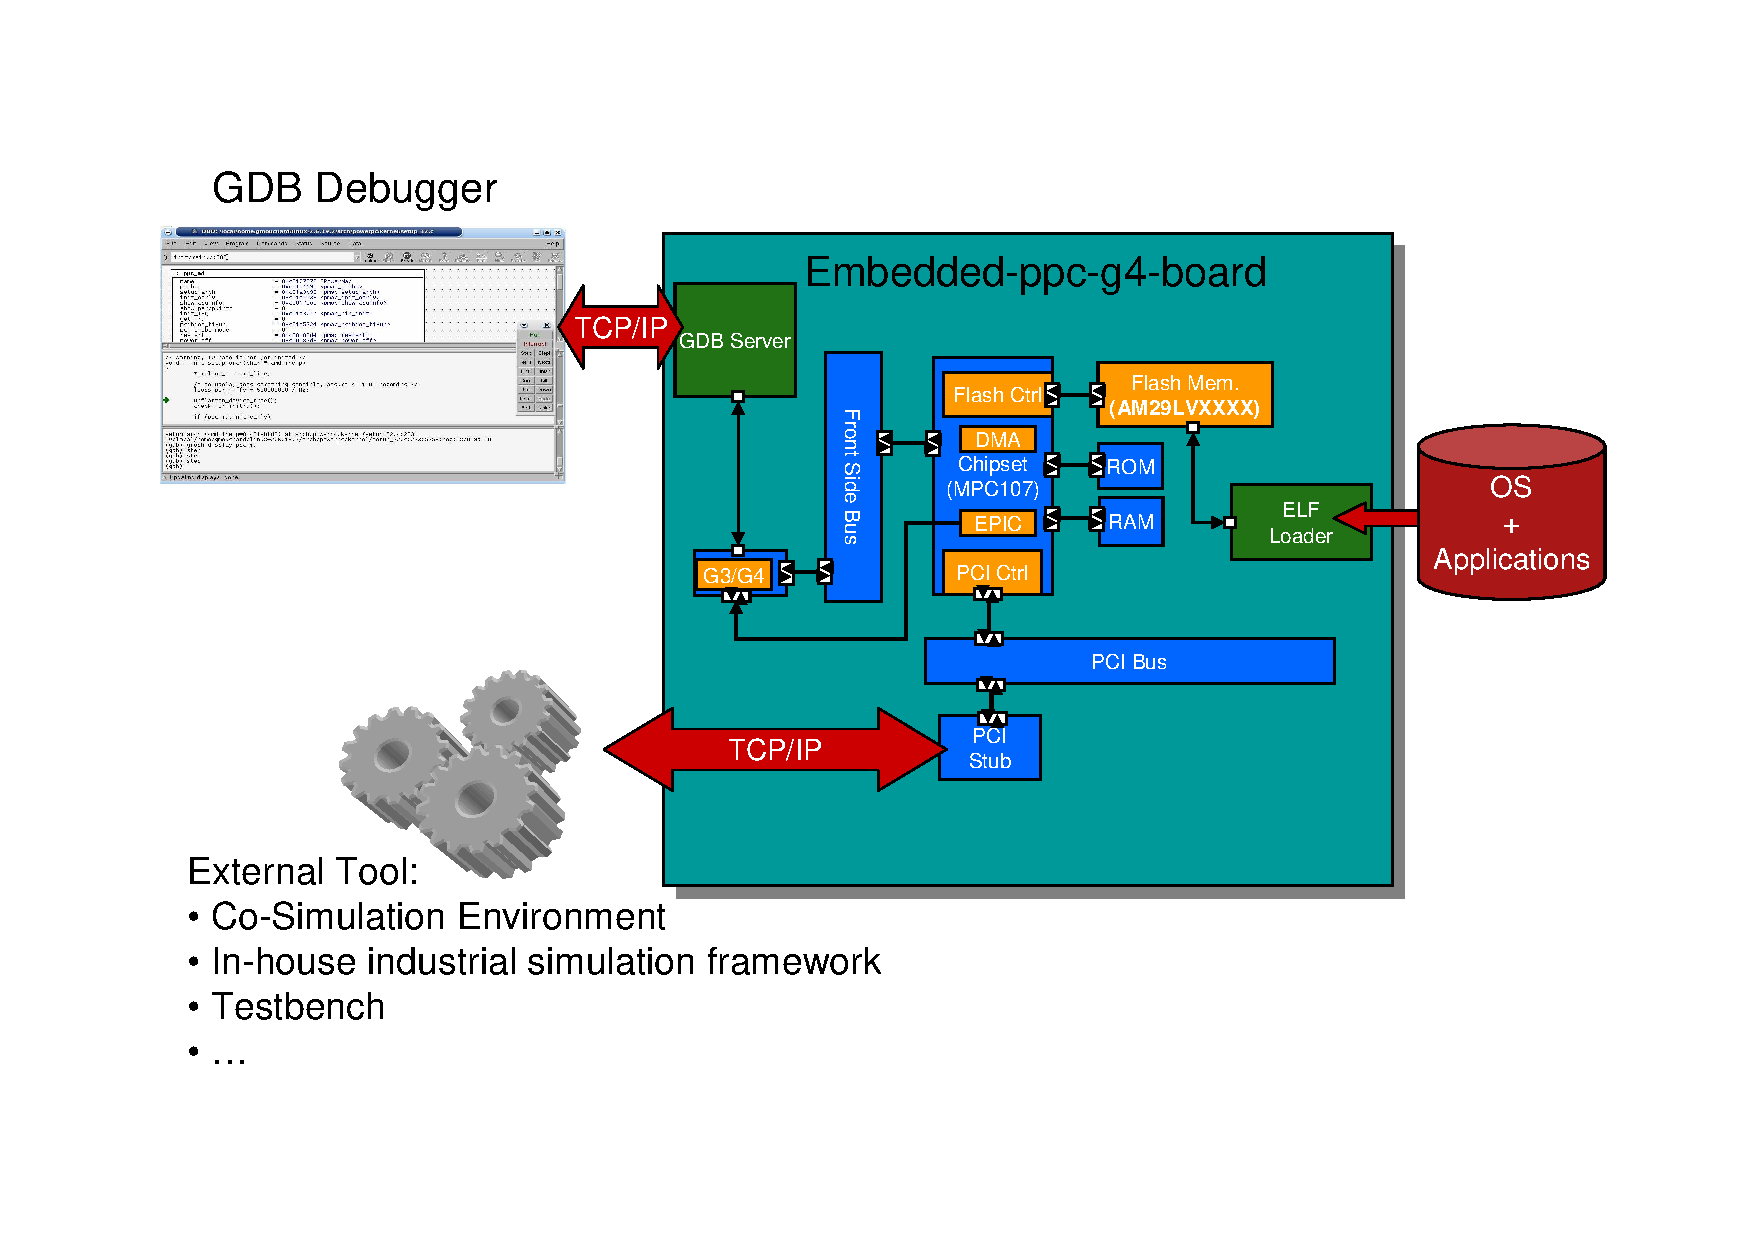
\includegraphics[width=\textwidth]{embedded_ppc_g4_board/fig_schematic.pdf}
	\end{center}
	\caption{UNISIM embedded-ppc-g4-board simulator schematic.}
\end{figure}
\noindent The UNISIM embedded-ppc-g4-board simulator is composed of the following modules and services:
\begin{itemize}\addtolength{\itemsep}{-0.40\baselineskip}
\item \textbf{bus}: Front side bus
\item \textbf{cpu}: PowerPC MPC7447A CPU
\item \textbf{debugger}
\item \textbf{erom}: Memory
\item \textbf{flash}: This module implements an AM29LV800BT flash memory with the following characteristics:\\
Manufacturer ID: 0x010000\\
Device ID word \#0: 0xda2202\\
Size: 4194304 bytes\\
I/O width: 64 bits\\
Number of chips: 4 chips\\
I/O width per chip: 16 bits\\
Size per chip: 1048576 bytes\\
Number of Sectors: 19 sectors\\
8-bit mode support: yes\\
16-bit mode support: yes\\
Access time: 70 ns\\
Byte programming time: 9000 us\\
Word programming time: 110000 us\\
Sector erasing time: 700000000 us\\
Chip erasing time: 14000000000 us\\

\item \textbf{gdb-server}: this service implements the GDB server remote serial protocol over TCP/IP. Standards GDB clients (e.g. gdb, eclipse, ddd) can connect to the simulator to debug the target application that runs within the simulator.
\item \textbf{host-time}: this service is an abstraction layer for the host machine time
\item \textbf{inline-debugger}: this service implements a built-in debugger in the terminal console
\item \textbf{loader}: A multi-format loader that supports ELF32, ELF64, S19, COFF and Raw binary files
\item \textbf{loader.memory-mapper}: A memory mapper
\item \textbf{loader.tee-backtrace}: This service/client implements a tee ('T'). It unifies the backtrace capability of several services that individually provides their own backtrace capability
\item \textbf{loader.tee-blob}: This service/client implements a tee ('T'). It unifies the statement lookup capability of several services that individually provides their own statement lookup capability
\item \textbf{loader.tee-loader}: This service/client implements a tee ('T'). It unifies the loader capability of several services that individually provides their own loader capability
\item \textbf{loader.tee-stmt-lookup}: This service/client implements a tee ('T'). It unifies the statement lookup capability of several services that individually provides their own statement lookup capability
\item \textbf{loader.tee-symbol-table-lookup}: This service/client implements a tee ('T'). It unifies the symbol table lookup capability of several services that individually provides their own symbol table lookup capability
\item \textbf{memory}: Memory
\item \textbf{mpc107}: MPC107 chipset
\item \textbf{mpc107.DMA}: MPC107 integrated Direct Memory Access (DMA) controller
\item \textbf{mpc107.address\_mapper}: MPC107 Address mapper
\item \textbf{mpc107.atu}: MPC107 integrated Address Translation Unit (ATU)
\item \textbf{mpc107.epic}: MPC107 integrated Embedded Programmable Interrupt Controller (EPIC)
\item \textbf{mpc107.pci\_controller}: MPC107 integrated PCI bus controller
\item \textbf{pci-bus}: PCI bus
\item \textbf{pci-stub}: A module that implements a PCI target and acts as a co-simulation stub controlled over a TCP/IP or pipe connection.
\item \textbf{profiler}
\item \textbf{tee-memory-access-reporting}
\item \textbf{tee-memory-access-reporting.tee-memory-access-reporting.control\_selector[0]}
\item \textbf{tee-memory-access-reporting.tee-memory-access-reporting.control\_selector[10]}
\item \textbf{tee-memory-access-reporting.tee-memory-access-reporting.control\_selector[11]}
\item \textbf{tee-memory-access-reporting.tee-memory-access-reporting.control\_selector[12]}
\item \textbf{tee-memory-access-reporting.tee-memory-access-reporting.control\_selector[13]}
\item \textbf{tee-memory-access-reporting.tee-memory-access-reporting.control\_selector[14]}
\item \textbf{tee-memory-access-reporting.tee-memory-access-reporting.control\_selector[15]}
\item \textbf{tee-memory-access-reporting.tee-memory-access-reporting.control\_selector[1]}
\item \textbf{tee-memory-access-reporting.tee-memory-access-reporting.control\_selector[2]}
\item \textbf{tee-memory-access-reporting.tee-memory-access-reporting.control\_selector[3]}
\item \textbf{tee-memory-access-reporting.tee-memory-access-reporting.control\_selector[4]}
\item \textbf{tee-memory-access-reporting.tee-memory-access-reporting.control\_selector[5]}
\item \textbf{tee-memory-access-reporting.tee-memory-access-reporting.control\_selector[6]}
\item \textbf{tee-memory-access-reporting.tee-memory-access-reporting.control\_selector[7]}
\item \textbf{tee-memory-access-reporting.tee-memory-access-reporting.control\_selector[8]}
\item \textbf{tee-memory-access-reporting.tee-memory-access-reporting.control\_selector[9]}
\item \textbf{tee-symbol-table-lookup}: This service/client implements a tee ('T'). It unifies the symbol table lookup capability of several services that individually provides their own symbol table lookup capability
\item \textbf{time}: this service is an abstraction layer for the SystemC kernel time
\end{itemize}
\subsection{Using the UNISIM embedded-ppc-g4-board simulator}
\label{UNISIM embedded-ppc-g4-board_using}
The UNISIM embedded-ppc-g4-board simulator has the following command line options:\\
~\\
\noindent Usage: \texttt{unisim-embedded-ppc-g4-board-1.1beta4 [<options>] [...]}

\noindent Options:
\begin{itemize}
\item \texttt{--set $<$param=value$>$ or -s $<$param=value$>$}: set value of parameter 'param' to 'value'
\item \texttt{--config $<$XML file$>$ or -c $<$XML file$>$}: configures the simulator with the given XML configuration file
\item \texttt{--get-config $<$XML file$>$ or -g $<$XML file$>$}: get the simulator configuration XML file (you can use it to create your own configuration. This option can be combined with -c to get a new configuration file with existing variables from another file
\item \texttt{--list or -l}: lists all available parameters, their type, and their current value
\item \texttt{--warn or -w}: enable printing of kernel warnings
\item \texttt{--doc $<$Latex file$>$ or -d $<$Latex file$>$}: enable printing a latex documentation
\item \texttt{--version or -v}: displays the program version information
\item \texttt{--share-path $<$path$>$ or -p $<$path$>$}: the path that should be used for the share directory (absolute path)
\item \texttt{--help or -h}: displays this help
\end{itemize}
\subsection{Configuration}
\label{UNISIM embedded-ppc-g4-board_configuration}
Simulator configuration (see below) can be modified using command line Options \texttt{--set $<$param=value$>$} or \texttt{--config $<$config file$>$}.\\
~\\
\tablehead{\hline}
\tabletail{\hline}
\begin{supertabular}{|p{7.5cm}|p{7.5cm}|}
\multicolumn{2}{|l|}{\textbf{\Large Global}}\\
\hline
\multicolumn{1}{|p{7.5cm}}{\textbf{Name:} \texttt{enable-gdb-server}} & \multicolumn{1}{p{7.5cm}|}{\textbf{Type:} \texttt{parameter}}\\
\multicolumn{1}{|p{7.5cm}}{\textbf{Default:} \texttt{true}} & \multicolumn{1}{p{7.5cm}|}{\textbf{Data type:} \texttt{boolean}}\\
\multicolumn{2}{|p{15cm}|}{\textbf{Valid:} \texttt{true},~\texttt{false}}\\
\multicolumn{2}{|l|}{}\\
\multicolumn{2}{|p{15cm}|}{\textbf{Description:} \newline Enable/Disable GDB server instantiation.}\\
\hline
\multicolumn{1}{|p{7.5cm}}{\textbf{Name:} \texttt{enable-inline-debugger}} & \multicolumn{1}{p{7.5cm}|}{\textbf{Type:} \texttt{parameter}}\\
\multicolumn{1}{|p{7.5cm}}{\textbf{Default:} \texttt{true}} & \multicolumn{1}{p{7.5cm}|}{\textbf{Data type:} \texttt{boolean}}\\
\multicolumn{2}{|p{15cm}|}{\textbf{Valid:} \texttt{true},~\texttt{false}}\\
\multicolumn{2}{|l|}{}\\
\multicolumn{2}{|p{15cm}|}{\textbf{Description:} \newline Enable/Disable inline debugger instantiation.}\\
\hline
\multicolumn{1}{|p{7.5cm}}{\textbf{Name:} \texttt{enable-press-enter-at-exit}} & \multicolumn{1}{p{7.5cm}|}{\textbf{Type:} \texttt{parameter}}\\
\multicolumn{1}{|p{7.5cm}}{\textbf{Default:} \texttt{false}} & \multicolumn{1}{p{7.5cm}|}{\textbf{Data type:} \texttt{boolean}}\\
\multicolumn{2}{|p{15cm}|}{\textbf{Valid:} \texttt{true},~\texttt{false}}\\
\multicolumn{2}{|l|}{}\\
\multicolumn{2}{|p{15cm}|}{\textbf{Description:} \newline Enable/Disable pressing key enter at exit.}\\
\hline
\multicolumn{1}{|p{7.5cm}}{\textbf{Name:} \texttt{estimate-power}} & \multicolumn{1}{p{7.5cm}|}{\textbf{Type:} \texttt{parameter}}\\
\multicolumn{1}{|p{7.5cm}}{\textbf{Default:} \texttt{false}} & \multicolumn{1}{p{7.5cm}|}{\textbf{Data type:} \texttt{boolean}}\\
\multicolumn{2}{|p{15cm}|}{\textbf{Valid:} \texttt{true},~\texttt{false}}\\
\multicolumn{2}{|l|}{}\\
\multicolumn{2}{|p{15cm}|}{\textbf{Description:} \newline Enable/Disable power estimators instantiation.}\\
\hline
\multicolumn{1}{|p{7.5cm}}{\textbf{Name:} \texttt{kernel\_logger.file}} & \multicolumn{1}{p{7.5cm}|}{\textbf{Type:} \texttt{parameter}}\\
\multicolumn{1}{|p{7.5cm}}{\textbf{Default:} \texttt{false}} & \multicolumn{1}{p{7.5cm}|}{\textbf{Data type:} \texttt{boolean}}\\
\multicolumn{2}{|p{15cm}|}{\textbf{Valid:} \texttt{true},~\texttt{false}}\\
\multicolumn{2}{|l|}{}\\
\multicolumn{2}{|p{15cm}|}{\textbf{Description:} \newline Keep logger output in a file.}\\
\hline
\multicolumn{1}{|p{7.5cm}}{\textbf{Name:} \texttt{kernel\_logger.filename}} & \multicolumn{1}{p{7.5cm}|}{\textbf{Type:} \texttt{parameter}}\\
\multicolumn{1}{|p{7.5cm}}{\textbf{Default:} \texttt{logger\_output.txt}} & \multicolumn{1}{p{7.5cm}|}{\textbf{Data type:} \texttt{string}}\\
\multicolumn{2}{|l|}{}\\
\multicolumn{2}{|l|}{}\\
\multicolumn{2}{|p{15cm}|}{\textbf{Description:} \newline Filename to keep logger output \_(the option file must be activated).}\\
\hline
\multicolumn{1}{|p{7.5cm}}{\textbf{Name:} \texttt{kernel\_logger.std\_err}} & \multicolumn{1}{p{7.5cm}|}{\textbf{Type:} \texttt{parameter}}\\
\multicolumn{1}{|p{7.5cm}}{\textbf{Default:} \texttt{true}} & \multicolumn{1}{p{7.5cm}|}{\textbf{Data type:} \texttt{boolean}}\\
\multicolumn{2}{|p{15cm}|}{\textbf{Valid:} \texttt{true},~\texttt{false}}\\
\multicolumn{2}{|l|}{}\\
\multicolumn{2}{|p{15cm}|}{\textbf{Description:} \newline Show logger output through the standard error output.}\\
\hline
\multicolumn{1}{|p{7.5cm}}{\textbf{Name:} \texttt{kernel\_logger.std\_err\_color}} & \multicolumn{1}{p{7.5cm}|}{\textbf{Type:} \texttt{parameter}}\\
\multicolumn{1}{|p{7.5cm}}{\textbf{Default:} \texttt{false}} & \multicolumn{1}{p{7.5cm}|}{\textbf{Data type:} \texttt{boolean}}\\
\multicolumn{2}{|p{15cm}|}{\textbf{Valid:} \texttt{true},~\texttt{false}}\\
\multicolumn{2}{|l|}{}\\
\multicolumn{2}{|p{15cm}|}{\textbf{Description:} \newline Colorize logger output through the standard error output \_(only works if std\_err is active).}\\
\hline
\multicolumn{1}{|p{7.5cm}}{\textbf{Name:} \texttt{kernel\_logger.std\_out}} & \multicolumn{1}{p{7.5cm}|}{\textbf{Type:} \texttt{parameter}}\\
\multicolumn{1}{|p{7.5cm}}{\textbf{Default:} \texttt{false}} & \multicolumn{1}{p{7.5cm}|}{\textbf{Data type:} \texttt{boolean}}\\
\multicolumn{2}{|p{15cm}|}{\textbf{Valid:} \texttt{true},~\texttt{false}}\\
\multicolumn{2}{|l|}{}\\
\multicolumn{2}{|p{15cm}|}{\textbf{Description:} \newline Show logger output through the standard output.}\\
\hline
\multicolumn{1}{|p{7.5cm}}{\textbf{Name:} \texttt{kernel\_logger.std\_out\_color}} & \multicolumn{1}{p{7.5cm}|}{\textbf{Type:} \texttt{parameter}}\\
\multicolumn{1}{|p{7.5cm}}{\textbf{Default:} \texttt{false}} & \multicolumn{1}{p{7.5cm}|}{\textbf{Data type:} \texttt{boolean}}\\
\multicolumn{2}{|p{15cm}|}{\textbf{Valid:} \texttt{true},~\texttt{false}}\\
\multicolumn{2}{|l|}{}\\
\multicolumn{2}{|p{15cm}|}{\textbf{Description:} \newline Colorize logger output through the standard output \_(only works if std\_out is active).}\\
\hline
\multicolumn{1}{|p{7.5cm}}{\textbf{Name:} \texttt{kernel\_logger.xml\_file}} & \multicolumn{1}{p{7.5cm}|}{\textbf{Type:} \texttt{parameter}}\\
\multicolumn{1}{|p{7.5cm}}{\textbf{Default:} \texttt{false}} & \multicolumn{1}{p{7.5cm}|}{\textbf{Data type:} \texttt{boolean}}\\
\multicolumn{2}{|p{15cm}|}{\textbf{Valid:} \texttt{true},~\texttt{false}}\\
\multicolumn{2}{|l|}{}\\
\multicolumn{2}{|p{15cm}|}{\textbf{Description:} \newline Keep logger output in a file xml formatted.}\\
\hline
\multicolumn{1}{|p{7.5cm}}{\textbf{Name:} \texttt{kernel\_logger.xml\_file\_gzipped}} & \multicolumn{1}{p{7.5cm}|}{\textbf{Type:} \texttt{parameter}}\\
\multicolumn{1}{|p{7.5cm}}{\textbf{Default:} \texttt{false}} & \multicolumn{1}{p{7.5cm}|}{\textbf{Data type:} \texttt{boolean}}\\
\multicolumn{2}{|p{15cm}|}{\textbf{Valid:} \texttt{true},~\texttt{false}}\\
\multicolumn{2}{|l|}{}\\
\multicolumn{2}{|p{15cm}|}{\textbf{Description:} \newline If the xml\_file option is active, the output file will be compressed (a .gz extension will be automatically added to the xml\_filename option.}\\
\hline
\multicolumn{1}{|p{7.5cm}}{\textbf{Name:} \texttt{kernel\_logger.xml\_filename}} & \multicolumn{1}{p{7.5cm}|}{\textbf{Type:} \texttt{parameter}}\\
\multicolumn{1}{|p{7.5cm}}{\textbf{Default:} \texttt{logger\_output.xml}} & \multicolumn{1}{p{7.5cm}|}{\textbf{Data type:} \texttt{string}}\\
\multicolumn{2}{|l|}{}\\
\multicolumn{2}{|l|}{}\\
\multicolumn{2}{|p{15cm}|}{\textbf{Description:} \newline Filename to keep logger xml output \_(the option xml\_file must be activated).}\\
\hline
\multicolumn{1}{|p{7.5cm}}{\textbf{Name:} \texttt{message-spy}} & \multicolumn{1}{p{7.5cm}|}{\textbf{Type:} \texttt{parameter}}\\
\multicolumn{1}{|p{7.5cm}}{\textbf{Default:} \texttt{false}} & \multicolumn{1}{p{7.5cm}|}{\textbf{Data type:} \texttt{boolean}}\\
\multicolumn{2}{|p{15cm}|}{\textbf{Valid:} \texttt{true},~\texttt{false}}\\
\multicolumn{2}{|l|}{}\\
\multicolumn{2}{|p{15cm}|}{\textbf{Description:} \newline Enable/Disable message spies instantiation.}\\
\hline
\hline
\multicolumn{2}{|l|}{\textbf{\Large bus}}\\
\hline
\multicolumn{1}{|p{7.5cm}}{\textbf{Name:} \texttt{bus.verbose}} & \multicolumn{1}{p{7.5cm}|}{\textbf{Type:} \texttt{parameter}}\\
\multicolumn{1}{|p{7.5cm}}{\textbf{Default:} \texttt{false}} & \multicolumn{1}{p{7.5cm}|}{\textbf{Data type:} \texttt{boolean}}\\
\multicolumn{2}{|p{15cm}|}{\textbf{Valid:} \texttt{true},~\texttt{false}}\\
\multicolumn{2}{|l|}{}\\
\multicolumn{2}{|p{15cm}|}{\textbf{Description:} \newline enable/disable verbosity.}\\
\hline
\multicolumn{1}{|p{7.5cm}}{\textbf{Name:} \texttt{bus.cycle-time}} & \multicolumn{1}{p{7.5cm}|}{\textbf{Type:} \texttt{parameter}}\\
\multicolumn{1}{|p{7.5cm}}{\textbf{Default:} \texttt{13332 ps}} & \multicolumn{1}{p{7.5cm}|}{\textbf{Data type:} \texttt{sc\_time}}\\
\multicolumn{2}{|l|}{}\\
\multicolumn{2}{|l|}{}\\
\multicolumn{2}{|p{15cm}|}{\textbf{Description:} \newline cycle time.}\\
\hline
\hline
\multicolumn{2}{|l|}{\textbf{\Large cpu}}\\
\hline
\multicolumn{1}{|p{7.5cm}}{\textbf{Name:} \texttt{cpu.cpu-cycle-time}} & \multicolumn{1}{p{7.5cm}|}{\textbf{Type:} \texttt{parameter}}\\
\multicolumn{1}{|p{7.5cm}}{\textbf{Default:} \texttt{3333}} & \multicolumn{1}{p{7.5cm}|}{\textbf{Data type:} \texttt{unsigned 64-bit integer}}\\
\multicolumn{2}{|l|}{}\\
\multicolumn{2}{|l|}{}\\
\multicolumn{2}{|p{15cm}|}{\textbf{Description:} \newline CPU cycle time in picoseconds.}\\
\hline
\multicolumn{1}{|p{7.5cm}}{\textbf{Name:} \texttt{cpu.voltage}} & \multicolumn{1}{p{7.5cm}|}{\textbf{Type:} \texttt{parameter}}\\
\multicolumn{1}{|p{7.5cm}}{\textbf{Default:} \texttt{1300}} & \multicolumn{1}{p{7.5cm}|}{\textbf{Data type:} \texttt{unsigned 64-bit integer}}\\
\multicolumn{2}{|l|}{}\\
\multicolumn{2}{|l|}{}\\
\multicolumn{2}{|p{15cm}|}{\textbf{Description:} \newline CPU voltage in mV.}\\
\hline
\multicolumn{1}{|p{7.5cm}}{\textbf{Name:} \texttt{cpu.max-inst}} & \multicolumn{1}{p{7.5cm}|}{\textbf{Type:} \texttt{parameter}}\\
\multicolumn{1}{|p{7.5cm}}{\textbf{Default:} \texttt{18446744073709551615}} & \multicolumn{1}{p{7.5cm}|}{\textbf{Data type:} \texttt{unsigned 64-bit integer}}\\
\multicolumn{2}{|l|}{}\\
\multicolumn{2}{|l|}{}\\
\multicolumn{2}{|p{15cm}|}{\textbf{Description:} \newline maximum number of instructions to simulate.}\\
\hline
\multicolumn{1}{|p{7.5cm}}{\textbf{Name:} \texttt{cpu.verbose-all}} & \multicolumn{1}{p{7.5cm}|}{\textbf{Type:} \texttt{parameter}}\\
\multicolumn{1}{|p{7.5cm}}{\textbf{Default:} \texttt{false}} & \multicolumn{1}{p{7.5cm}|}{\textbf{Data type:} \texttt{boolean}}\\
\multicolumn{2}{|p{15cm}|}{\textbf{Valid:} \texttt{true},~\texttt{false}}\\
\multicolumn{2}{|l|}{}\\
\multicolumn{2}{|p{15cm}|}{\textbf{Description:} \newline globally enable/disable verbosity.}\\
\hline
\multicolumn{1}{|p{7.5cm}}{\textbf{Name:} \texttt{cpu.verbose-setup}} & \multicolumn{1}{p{7.5cm}|}{\textbf{Type:} \texttt{parameter}}\\
\multicolumn{1}{|p{7.5cm}}{\textbf{Default:} \texttt{false}} & \multicolumn{1}{p{7.5cm}|}{\textbf{Data type:} \texttt{boolean}}\\
\multicolumn{2}{|p{15cm}|}{\textbf{Valid:} \texttt{true},~\texttt{false}}\\
\multicolumn{2}{|l|}{}\\
\multicolumn{2}{|p{15cm}|}{\textbf{Description:} \newline enable/disable verbosity while setup.}\\
\hline
\multicolumn{1}{|p{7.5cm}}{\textbf{Name:} \texttt{cpu.verbose-step}} & \multicolumn{1}{p{7.5cm}|}{\textbf{Type:} \texttt{parameter}}\\
\multicolumn{1}{|p{7.5cm}}{\textbf{Default:} \texttt{false}} & \multicolumn{1}{p{7.5cm}|}{\textbf{Data type:} \texttt{boolean}}\\
\multicolumn{2}{|p{15cm}|}{\textbf{Valid:} \texttt{true},~\texttt{false}}\\
\multicolumn{2}{|l|}{}\\
\multicolumn{2}{|p{15cm}|}{\textbf{Description:} \newline enable/disable verbosity when simulating an instruction.}\\
\hline
\multicolumn{1}{|p{7.5cm}}{\textbf{Name:} \texttt{cpu.verbose-dtlb}} & \multicolumn{1}{p{7.5cm}|}{\textbf{Type:} \texttt{parameter}}\\
\multicolumn{1}{|p{7.5cm}}{\textbf{Default:} \texttt{false}} & \multicolumn{1}{p{7.5cm}|}{\textbf{Data type:} \texttt{boolean}}\\
\multicolumn{2}{|p{15cm}|}{\textbf{Valid:} \texttt{true},~\texttt{false}}\\
\multicolumn{2}{|l|}{}\\
\multicolumn{2}{|p{15cm}|}{\textbf{Description:} \newline enable/disable verbosity when accessing data translation lookahead buffer.}\\
\hline
\multicolumn{1}{|p{7.5cm}}{\textbf{Name:} \texttt{cpu.verbose-itlb}} & \multicolumn{1}{p{7.5cm}|}{\textbf{Type:} \texttt{parameter}}\\
\multicolumn{1}{|p{7.5cm}}{\textbf{Default:} \texttt{false}} & \multicolumn{1}{p{7.5cm}|}{\textbf{Data type:} \texttt{boolean}}\\
\multicolumn{2}{|p{15cm}|}{\textbf{Valid:} \texttt{true},~\texttt{false}}\\
\multicolumn{2}{|l|}{}\\
\multicolumn{2}{|p{15cm}|}{\textbf{Description:} \newline enable/disable verbosity when accessing instruction translation lookahead buffer.}\\
\hline
\multicolumn{1}{|p{7.5cm}}{\textbf{Name:} \texttt{cpu.verbose-dl1}} & \multicolumn{1}{p{7.5cm}|}{\textbf{Type:} \texttt{parameter}}\\
\multicolumn{1}{|p{7.5cm}}{\textbf{Default:} \texttt{false}} & \multicolumn{1}{p{7.5cm}|}{\textbf{Data type:} \texttt{boolean}}\\
\multicolumn{2}{|p{15cm}|}{\textbf{Valid:} \texttt{true},~\texttt{false}}\\
\multicolumn{2}{|l|}{}\\
\multicolumn{2}{|p{15cm}|}{\textbf{Description:} \newline enable/disable verbosity when accessing L1 data cache.}\\
\hline
\multicolumn{1}{|p{7.5cm}}{\textbf{Name:} \texttt{cpu.verbose-il1}} & \multicolumn{1}{p{7.5cm}|}{\textbf{Type:} \texttt{parameter}}\\
\multicolumn{1}{|p{7.5cm}}{\textbf{Default:} \texttt{false}} & \multicolumn{1}{p{7.5cm}|}{\textbf{Data type:} \texttt{boolean}}\\
\multicolumn{2}{|p{15cm}|}{\textbf{Valid:} \texttt{true},~\texttt{false}}\\
\multicolumn{2}{|l|}{}\\
\multicolumn{2}{|p{15cm}|}{\textbf{Description:} \newline enable/disable verbosity when accessing L1 instruction cache.}\\
\hline
\multicolumn{1}{|p{7.5cm}}{\textbf{Name:} \texttt{cpu.verbose-l2}} & \multicolumn{1}{p{7.5cm}|}{\textbf{Type:} \texttt{parameter}}\\
\multicolumn{1}{|p{7.5cm}}{\textbf{Default:} \texttt{false}} & \multicolumn{1}{p{7.5cm}|}{\textbf{Data type:} \texttt{boolean}}\\
\multicolumn{2}{|p{15cm}|}{\textbf{Valid:} \texttt{true},~\texttt{false}}\\
\multicolumn{2}{|l|}{}\\
\multicolumn{2}{|p{15cm}|}{\textbf{Description:} \newline enable/disable verbosity when accessing L2 unified cache.}\\
\hline
\multicolumn{1}{|p{7.5cm}}{\textbf{Name:} \texttt{cpu.verbose-load}} & \multicolumn{1}{p{7.5cm}|}{\textbf{Type:} \texttt{parameter}}\\
\multicolumn{1}{|p{7.5cm}}{\textbf{Default:} \texttt{false}} & \multicolumn{1}{p{7.5cm}|}{\textbf{Data type:} \texttt{boolean}}\\
\multicolumn{2}{|p{15cm}|}{\textbf{Valid:} \texttt{true},~\texttt{false}}\\
\multicolumn{2}{|l|}{}\\
\multicolumn{2}{|p{15cm}|}{\textbf{Description:} \newline enable/disable verbosity when simulating a load.}\\
\hline
\multicolumn{1}{|p{7.5cm}}{\textbf{Name:} \texttt{cpu.verbose-store}} & \multicolumn{1}{p{7.5cm}|}{\textbf{Type:} \texttt{parameter}}\\
\multicolumn{1}{|p{7.5cm}}{\textbf{Default:} \texttt{false}} & \multicolumn{1}{p{7.5cm}|}{\textbf{Data type:} \texttt{boolean}}\\
\multicolumn{2}{|p{15cm}|}{\textbf{Valid:} \texttt{true},~\texttt{false}}\\
\multicolumn{2}{|l|}{}\\
\multicolumn{2}{|p{15cm}|}{\textbf{Description:} \newline enable/disable verbosity when simulating a store.}\\
\hline
\multicolumn{1}{|p{7.5cm}}{\textbf{Name:} \texttt{cpu.verbose-read-memory}} & \multicolumn{1}{p{7.5cm}|}{\textbf{Type:} \texttt{parameter}}\\
\multicolumn{1}{|p{7.5cm}}{\textbf{Default:} \texttt{false}} & \multicolumn{1}{p{7.5cm}|}{\textbf{Data type:} \texttt{boolean}}\\
\multicolumn{2}{|p{15cm}|}{\textbf{Valid:} \texttt{true},~\texttt{false}}\\
\multicolumn{2}{|l|}{}\\
\multicolumn{2}{|p{15cm}|}{\textbf{Description:} \newline enable/disable verbosity when reading memory for a debug purpose.}\\
\hline
\multicolumn{1}{|p{7.5cm}}{\textbf{Name:} \texttt{cpu.verbose-write-memory}} & \multicolumn{1}{p{7.5cm}|}{\textbf{Type:} \texttt{parameter}}\\
\multicolumn{1}{|p{7.5cm}}{\textbf{Default:} \texttt{false}} & \multicolumn{1}{p{7.5cm}|}{\textbf{Data type:} \texttt{boolean}}\\
\multicolumn{2}{|p{15cm}|}{\textbf{Valid:} \texttt{true},~\texttt{false}}\\
\multicolumn{2}{|l|}{}\\
\multicolumn{2}{|p{15cm}|}{\textbf{Description:} \newline enable/disable verbosity when writing memory for a debug purpose.}\\
\hline
\multicolumn{1}{|p{7.5cm}}{\textbf{Name:} \texttt{cpu.verbose-exception}} & \multicolumn{1}{p{7.5cm}|}{\textbf{Type:} \texttt{parameter}}\\
\multicolumn{1}{|p{7.5cm}}{\textbf{Default:} \texttt{false}} & \multicolumn{1}{p{7.5cm}|}{\textbf{Data type:} \texttt{boolean}}\\
\multicolumn{2}{|p{15cm}|}{\textbf{Valid:} \texttt{true},~\texttt{false}}\\
\multicolumn{2}{|l|}{}\\
\multicolumn{2}{|p{15cm}|}{\textbf{Description:} \newline enable/disable verbosity when handling exceptions.}\\
\hline
\multicolumn{1}{|p{7.5cm}}{\textbf{Name:} \texttt{cpu.verbose-set-msr}} & \multicolumn{1}{p{7.5cm}|}{\textbf{Type:} \texttt{parameter}}\\
\multicolumn{1}{|p{7.5cm}}{\textbf{Default:} \texttt{false}} & \multicolumn{1}{p{7.5cm}|}{\textbf{Data type:} \texttt{boolean}}\\
\multicolumn{2}{|p{15cm}|}{\textbf{Valid:} \texttt{true},~\texttt{false}}\\
\multicolumn{2}{|l|}{}\\
\multicolumn{2}{|p{15cm}|}{\textbf{Description:} \newline enable/disable verbosity when setting MSR.}\\
\hline
\multicolumn{1}{|p{7.5cm}}{\textbf{Name:} \texttt{cpu.verbose-set-hid0}} & \multicolumn{1}{p{7.5cm}|}{\textbf{Type:} \texttt{parameter}}\\
\multicolumn{1}{|p{7.5cm}}{\textbf{Default:} \texttt{false}} & \multicolumn{1}{p{7.5cm}|}{\textbf{Data type:} \texttt{boolean}}\\
\multicolumn{2}{|p{15cm}|}{\textbf{Valid:} \texttt{true},~\texttt{false}}\\
\multicolumn{2}{|l|}{}\\
\multicolumn{2}{|p{15cm}|}{\textbf{Description:} \newline enable/disable verbosity when setting HID0.}\\
\hline
\multicolumn{1}{|p{7.5cm}}{\textbf{Name:} \texttt{cpu.verbose-set-hid1}} & \multicolumn{1}{p{7.5cm}|}{\textbf{Type:} \texttt{parameter}}\\
\multicolumn{1}{|p{7.5cm}}{\textbf{Default:} \texttt{false}} & \multicolumn{1}{p{7.5cm}|}{\textbf{Data type:} \texttt{boolean}}\\
\multicolumn{2}{|p{15cm}|}{\textbf{Valid:} \texttt{true},~\texttt{false}}\\
\multicolumn{2}{|l|}{}\\
\multicolumn{2}{|p{15cm}|}{\textbf{Description:} \newline enable/disable verbosity when setting HID1.}\\
\hline
\multicolumn{1}{|p{7.5cm}}{\textbf{Name:} \texttt{cpu.verbose-set-hid2}} & \multicolumn{1}{p{7.5cm}|}{\textbf{Type:} \texttt{parameter}}\\
\multicolumn{1}{|p{7.5cm}}{\textbf{Default:} \texttt{false}} & \multicolumn{1}{p{7.5cm}|}{\textbf{Data type:} \texttt{boolean}}\\
\multicolumn{2}{|p{15cm}|}{\textbf{Valid:} \texttt{true},~\texttt{false}}\\
\multicolumn{2}{|l|}{}\\
\multicolumn{2}{|p{15cm}|}{\textbf{Description:} \newline enable/disable verbosity when setting HID2.}\\
\hline
\multicolumn{1}{|p{7.5cm}}{\textbf{Name:} \texttt{cpu.verbose-set-l2cr}} & \multicolumn{1}{p{7.5cm}|}{\textbf{Type:} \texttt{parameter}}\\
\multicolumn{1}{|p{7.5cm}}{\textbf{Default:} \texttt{false}} & \multicolumn{1}{p{7.5cm}|}{\textbf{Data type:} \texttt{boolean}}\\
\multicolumn{2}{|p{15cm}|}{\textbf{Valid:} \texttt{true},~\texttt{false}}\\
\multicolumn{2}{|l|}{}\\
\multicolumn{2}{|p{15cm}|}{\textbf{Description:} \newline enable/disable verbosity when setting L2CR.}\\
\hline
\multicolumn{1}{|p{7.5cm}}{\textbf{Name:} \texttt{cpu.enable-linux-printk-snooping}} & \multicolumn{1}{p{7.5cm}|}{\textbf{Type:} \texttt{parameter}}\\
\multicolumn{1}{|p{7.5cm}}{\textbf{Default:} \texttt{false}} & \multicolumn{1}{p{7.5cm}|}{\textbf{Data type:} \texttt{boolean}}\\
\multicolumn{2}{|p{15cm}|}{\textbf{Valid:} \texttt{true},~\texttt{false}}\\
\multicolumn{2}{|l|}{}\\
\multicolumn{2}{|p{15cm}|}{\textbf{Description:} \newline enable/disable linux printk buffer snooping.}\\
\hline
\multicolumn{1}{|p{7.5cm}}{\textbf{Name:} \texttt{cpu.enable-linux-syscall-snooping}} & \multicolumn{1}{p{7.5cm}|}{\textbf{Type:} \texttt{parameter}}\\
\multicolumn{1}{|p{7.5cm}}{\textbf{Default:} \texttt{false}} & \multicolumn{1}{p{7.5cm}|}{\textbf{Data type:} \texttt{boolean}}\\
\multicolumn{2}{|p{15cm}|}{\textbf{Valid:} \texttt{true},~\texttt{false}}\\
\multicolumn{2}{|l|}{}\\
\multicolumn{2}{|p{15cm}|}{\textbf{Description:} \newline enable/disable linux syscall snooping.}\\
\hline
\multicolumn{1}{|p{7.5cm}}{\textbf{Name:} \texttt{cpu.trap-on-instruction-counter}} & \multicolumn{1}{p{7.5cm}|}{\textbf{Type:} \texttt{parameter}}\\
\multicolumn{1}{|p{7.5cm}}{\textbf{Default:} \texttt{18446744073709551615}} & \multicolumn{1}{p{7.5cm}|}{\textbf{Data type:} \texttt{unsigned 64-bit integer}}\\
\multicolumn{2}{|l|}{}\\
\multicolumn{2}{|l|}{}\\
\multicolumn{2}{|p{15cm}|}{\textbf{Description:} \newline number of simulated instruction before traping.}\\
\hline
\multicolumn{1}{|p{7.5cm}}{\textbf{Name:} \texttt{cpu.halt-on}} & \multicolumn{1}{p{7.5cm}|}{\textbf{Type:} \texttt{parameter}}\\
\multicolumn{1}{|p{7.5cm}}{\textbf{Default:} \texttt{}} & \multicolumn{1}{p{7.5cm}|}{\textbf{Data type:} \texttt{string}}\\
\multicolumn{2}{|l|}{}\\
\multicolumn{2}{|l|}{}\\
\multicolumn{2}{|p{15cm}|}{\textbf{Description:} \newline Symbol or address where to stop simulation.}\\
\hline
\multicolumn{1}{|p{7.5cm}}{\textbf{Name:} \texttt{cpu.bus-cycle-time}} & \multicolumn{1}{p{7.5cm}|}{\textbf{Type:} \texttt{parameter}}\\
\multicolumn{1}{|p{7.5cm}}{\textbf{Default:} \texttt{13332 ps}} & \multicolumn{1}{p{7.5cm}|}{\textbf{Data type:} \texttt{sc\_time}}\\
\multicolumn{2}{|l|}{}\\
\multicolumn{2}{|l|}{}\\
\multicolumn{2}{|p{15cm}|}{\textbf{Description:} \newline bus cycle time.}\\
\hline
\multicolumn{1}{|p{7.5cm}}{\textbf{Name:} \texttt{cpu.nice-time}} & \multicolumn{1}{p{7.5cm}|}{\textbf{Type:} \texttt{parameter}}\\
\multicolumn{1}{|p{7.5cm}}{\textbf{Default:} \texttt{1 ms}} & \multicolumn{1}{p{7.5cm}|}{\textbf{Data type:} \texttt{sc\_time}}\\
\multicolumn{2}{|l|}{}\\
\multicolumn{2}{|l|}{}\\
\multicolumn{2}{|p{15cm}|}{\textbf{Description:} \newline maximum time between synchonizations.}\\
\hline
\multicolumn{1}{|p{7.5cm}}{\textbf{Name:} \texttt{cpu.ipc}} & \multicolumn{1}{p{7.5cm}|}{\textbf{Type:} \texttt{parameter}}\\
\multicolumn{1}{|p{7.5cm}}{\textbf{Default:} \texttt{1}} & \multicolumn{1}{p{7.5cm}|}{\textbf{Data type:} \texttt{double precision floating-point}}\\
\multicolumn{2}{|l|}{}\\
\multicolumn{2}{|l|}{}\\
\multicolumn{2}{|p{15cm}|}{\textbf{Description:} \newline targeted average instructions per second.}\\
\hline
\multicolumn{1}{|p{7.5cm}}{\textbf{Name:} \texttt{cpu.enable-host-idle}} & \multicolumn{1}{p{7.5cm}|}{\textbf{Type:} \texttt{parameter}}\\
\multicolumn{1}{|p{7.5cm}}{\textbf{Default:} \texttt{false}} & \multicolumn{1}{p{7.5cm}|}{\textbf{Data type:} \texttt{boolean}}\\
\multicolumn{2}{|p{15cm}|}{\textbf{Valid:} \texttt{true},~\texttt{false}}\\
\multicolumn{2}{|l|}{}\\
\multicolumn{2}{|p{15cm}|}{\textbf{Description:} \newline Enable/Disable host idle periods when target is idle.}\\
\hline
\hline
\multicolumn{2}{|l|}{\textbf{\Large debugger}}\\
\hline
\multicolumn{1}{|p{7.5cm}}{\textbf{Name:} \texttt{debugger.verbose}} & \multicolumn{1}{p{7.5cm}|}{\textbf{Type:} \texttt{parameter}}\\
\multicolumn{1}{|p{7.5cm}}{\textbf{Default:} \texttt{false}} & \multicolumn{1}{p{7.5cm}|}{\textbf{Data type:} \texttt{boolean}}\\
\multicolumn{2}{|p{15cm}|}{\textbf{Valid:} \texttt{true},~\texttt{false}}\\
\multicolumn{2}{|l|}{}\\
\multicolumn{2}{|p{15cm}|}{\textbf{Description:} \newline Enable/Disable verbosity.}\\
\hline
\multicolumn{1}{|p{7.5cm}}{\textbf{Name:} \texttt{debugger.dwarf-to-html-output-} \newline$\hookrightarrow$\texttt{directory}} & \multicolumn{1}{p{7.5cm}|}{\textbf{Type:} \texttt{parameter}}\\
\multicolumn{1}{|p{7.5cm}}{\textbf{Default:} \texttt{}} & \multicolumn{1}{p{7.5cm}|}{\textbf{Data type:} \texttt{string}}\\
\multicolumn{2}{|l|}{}\\
\multicolumn{2}{|l|}{}\\
\multicolumn{2}{|p{15cm}|}{\textbf{Description:} \newline DWARF v2/v3 to HTML output directory.}\\
\hline
\multicolumn{1}{|p{7.5cm}}{\textbf{Name:} \texttt{debugger.dwarf-register-number-} \newline$\hookrightarrow$\texttt{mapping-filename}} & \multicolumn{1}{p{7.5cm}|}{\textbf{Type:} \texttt{parameter}}\\
\multicolumn{1}{|p{7.5cm}}{\textbf{Default:} \texttt{powerpc\_eabi\_gcc\_dwarf\_register\_} \newline$\hookrightarrow$\texttt{number\_mapping.xml}} & \multicolumn{1}{p{7.5cm}|}{\textbf{Data type:} \texttt{string}}\\
\multicolumn{2}{|l|}{}\\
\multicolumn{2}{|l|}{}\\
\multicolumn{2}{|p{15cm}|}{\textbf{Description:} \newline DWARF register number mapping filename.}\\
\hline
\multicolumn{1}{|p{7.5cm}}{\textbf{Name:} \texttt{debugger.parse-dwarf}} & \multicolumn{1}{p{7.5cm}|}{\textbf{Type:} \texttt{parameter}}\\
\multicolumn{1}{|p{7.5cm}}{\textbf{Default:} \texttt{true}} & \multicolumn{1}{p{7.5cm}|}{\textbf{Data type:} \texttt{boolean}}\\
\multicolumn{2}{|p{15cm}|}{\textbf{Valid:} \texttt{true},~\texttt{false}}\\
\multicolumn{2}{|l|}{}\\
\multicolumn{2}{|p{15cm}|}{\textbf{Description:} \newline Enable/Disable parsing of DWARF debugging informations.}\\
\hline
\multicolumn{1}{|p{7.5cm}}{\textbf{Name:} \texttt{debugger.debug-dwarf}} & \multicolumn{1}{p{7.5cm}|}{\textbf{Type:} \texttt{parameter}}\\
\multicolumn{1}{|p{7.5cm}}{\textbf{Default:} \texttt{false}} & \multicolumn{1}{p{7.5cm}|}{\textbf{Data type:} \texttt{boolean}}\\
\multicolumn{2}{|p{15cm}|}{\textbf{Valid:} \texttt{true},~\texttt{false}}\\
\multicolumn{2}{|l|}{}\\
\multicolumn{2}{|p{15cm}|}{\textbf{Description:} \newline Enable/Disable debugging of DWARF.}\\
\hline
\hline
\multicolumn{2}{|l|}{\textbf{\Large erom}}\\
\hline
\multicolumn{1}{|p{7.5cm}}{\textbf{Name:} \texttt{erom.org}} & \multicolumn{1}{p{7.5cm}|}{\textbf{Type:} \texttt{parameter}}\\
\multicolumn{1}{|p{7.5cm}}{\textbf{Default:} \texttt{0x78000000}} & \multicolumn{1}{p{7.5cm}|}{\textbf{Data type:} \texttt{unsigned 32-bit integer}}\\
\multicolumn{2}{|l|}{}\\
\multicolumn{2}{|l|}{}\\
\multicolumn{2}{|p{15cm}|}{\textbf{Description:} \newline memory origin/base address.}\\
\hline
\multicolumn{1}{|p{7.5cm}}{\textbf{Name:} \texttt{erom.bytesize}} & \multicolumn{1}{p{7.5cm}|}{\textbf{Type:} \texttt{parameter}}\\
\multicolumn{1}{|p{7.5cm}}{\textbf{Default:} \texttt{16777216}} & \multicolumn{1}{p{7.5cm}|}{\textbf{Data type:} \texttt{unsigned 32-bit integer}}\\
\multicolumn{2}{|l|}{}\\
\multicolumn{2}{|l|}{}\\
\multicolumn{2}{|p{15cm}|}{\textbf{Description:} \newline memory size in bytes.}\\
\hline
\multicolumn{1}{|p{7.5cm}}{\textbf{Name:} \texttt{erom.initial-byte-value}} & \multicolumn{1}{p{7.5cm}|}{\textbf{Type:} \texttt{parameter}}\\
\multicolumn{1}{|p{7.5cm}}{\textbf{Default:} \texttt{0x00}} & \multicolumn{1}{p{7.5cm}|}{\textbf{Data type:} \texttt{unsigned 8-bit integer}}\\
\multicolumn{2}{|l|}{}\\
\hline
\multicolumn{1}{|p{7.5cm}}{\textbf{Name:} \texttt{erom.verbose}} & \multicolumn{1}{p{7.5cm}|}{\textbf{Type:} \texttt{parameter}}\\
\multicolumn{1}{|p{7.5cm}}{\textbf{Default:} \texttt{false}} & \multicolumn{1}{p{7.5cm}|}{\textbf{Data type:} \texttt{boolean}}\\
\multicolumn{2}{|p{15cm}|}{\textbf{Valid:} \texttt{true},~\texttt{false}}\\
\multicolumn{2}{|l|}{}\\
\multicolumn{2}{|p{15cm}|}{\textbf{Description:} \newline enable/disable verbosity.}\\
\hline
\multicolumn{1}{|p{7.5cm}}{\textbf{Name:} \texttt{erom.cycle-time}} & \multicolumn{1}{p{7.5cm}|}{\textbf{Type:} \texttt{parameter}}\\
\multicolumn{1}{|p{7.5cm}}{\textbf{Default:} \texttt{13332 ps}} & \multicolumn{1}{p{7.5cm}|}{\textbf{Data type:} \texttt{sc\_time}}\\
\multicolumn{2}{|l|}{}\\
\multicolumn{2}{|l|}{}\\
\multicolumn{2}{|p{15cm}|}{\textbf{Description:} \newline RAM memory cycle time.}\\
\hline
\hline
\multicolumn{2}{|l|}{\textbf{\Large flash}}\\
\hline
\multicolumn{1}{|p{7.5cm}}{\textbf{Name:} \texttt{flash.verbose}} & \multicolumn{1}{p{7.5cm}|}{\textbf{Type:} \texttt{parameter}}\\
\multicolumn{1}{|p{7.5cm}}{\textbf{Default:} \texttt{false}} & \multicolumn{1}{p{7.5cm}|}{\textbf{Data type:} \texttt{boolean}}\\
\multicolumn{2}{|p{15cm}|}{\textbf{Valid:} \texttt{true},~\texttt{false}}\\
\multicolumn{2}{|l|}{}\\
\multicolumn{2}{|p{15cm}|}{\textbf{Description:} \newline enable/disable verbosity.}\\
\hline
\multicolumn{1}{|p{7.5cm}}{\textbf{Name:} \texttt{flash.org}} & \multicolumn{1}{p{7.5cm}|}{\textbf{Type:} \texttt{parameter}}\\
\multicolumn{1}{|p{7.5cm}}{\textbf{Default:} \texttt{0xff800000}} & \multicolumn{1}{p{7.5cm}|}{\textbf{Data type:} \texttt{unsigned 32-bit integer}}\\
\multicolumn{2}{|l|}{}\\
\multicolumn{2}{|l|}{}\\
\multicolumn{2}{|p{15cm}|}{\textbf{Description:} \newline flash memory base address.}\\
\hline
\multicolumn{1}{|p{7.5cm}}{\textbf{Name:} \texttt{flash.bytesize}} & \multicolumn{1}{p{7.5cm}|}{\textbf{Type:} \texttt{parameter}}\\
\multicolumn{1}{|p{7.5cm}}{\textbf{Default:} \texttt{8388608}} & \multicolumn{1}{p{7.5cm}|}{\textbf{Data type:} \texttt{unsigned 32-bit integer}}\\
\multicolumn{2}{|l|}{}\\
\multicolumn{2}{|l|}{}\\
\multicolumn{2}{|p{15cm}|}{\textbf{Description:} \newline flash memory size in bytes.}\\
\hline
\multicolumn{1}{|p{7.5cm}}{\textbf{Name:} \texttt{flash.endian}} & \multicolumn{1}{p{7.5cm}|}{\textbf{Type:} \texttt{parameter}}\\
\multicolumn{1}{|p{7.5cm}}{\textbf{Default:} \texttt{big-endian}} & \multicolumn{1}{p{7.5cm}|}{\textbf{Data type:} \texttt{endianess}}\\
\multicolumn{2}{|p{15cm}|}{\textbf{Valid:} \texttt{little-endian},~\texttt{big-endian}}\\
\multicolumn{2}{|l|}{}\\
\multicolumn{2}{|p{15cm}|}{\textbf{Description:} \newline endianness of flash memory.}\\
\hline
\multicolumn{1}{|p{7.5cm}}{\textbf{Name:} \texttt{flash.sector-protect[0]}} & \multicolumn{1}{p{7.5cm}|}{\textbf{Type:} \texttt{parameter}}\\
\multicolumn{1}{|p{7.5cm}}{\textbf{Default:} \texttt{false}} & \multicolumn{1}{p{7.5cm}|}{\textbf{Data type:} \texttt{boolean}}\\
\multicolumn{2}{|p{15cm}|}{\textbf{Valid:} \texttt{true},~\texttt{false}}\\
\multicolumn{2}{|l|}{}\\
\multicolumn{2}{|p{15cm}|}{\textbf{Description:} \newline enable/disable sector write protection.}\\
\hline
\multicolumn{1}{|p{7.5cm}}{\textbf{Name:} \texttt{flash.sector-protect[1]}} & \multicolumn{1}{p{7.5cm}|}{\textbf{Type:} \texttt{parameter}}\\
\multicolumn{1}{|p{7.5cm}}{\textbf{Default:} \texttt{false}} & \multicolumn{1}{p{7.5cm}|}{\textbf{Data type:} \texttt{boolean}}\\
\multicolumn{2}{|p{15cm}|}{\textbf{Valid:} \texttt{true},~\texttt{false}}\\
\multicolumn{2}{|l|}{}\\
\multicolumn{2}{|p{15cm}|}{\textbf{Description:} \newline enable/disable sector write protection.}\\
\hline
\multicolumn{1}{|p{7.5cm}}{\textbf{Name:} \texttt{flash.sector-protect[2]}} & \multicolumn{1}{p{7.5cm}|}{\textbf{Type:} \texttt{parameter}}\\
\multicolumn{1}{|p{7.5cm}}{\textbf{Default:} \texttt{false}} & \multicolumn{1}{p{7.5cm}|}{\textbf{Data type:} \texttt{boolean}}\\
\multicolumn{2}{|p{15cm}|}{\textbf{Valid:} \texttt{true},~\texttt{false}}\\
\multicolumn{2}{|l|}{}\\
\multicolumn{2}{|p{15cm}|}{\textbf{Description:} \newline enable/disable sector write protection.}\\
\hline
\multicolumn{1}{|p{7.5cm}}{\textbf{Name:} \texttt{flash.sector-protect[3]}} & \multicolumn{1}{p{7.5cm}|}{\textbf{Type:} \texttt{parameter}}\\
\multicolumn{1}{|p{7.5cm}}{\textbf{Default:} \texttt{false}} & \multicolumn{1}{p{7.5cm}|}{\textbf{Data type:} \texttt{boolean}}\\
\multicolumn{2}{|p{15cm}|}{\textbf{Valid:} \texttt{true},~\texttt{false}}\\
\multicolumn{2}{|l|}{}\\
\multicolumn{2}{|p{15cm}|}{\textbf{Description:} \newline enable/disable sector write protection.}\\
\hline
\multicolumn{1}{|p{7.5cm}}{\textbf{Name:} \texttt{flash.sector-protect[4]}} & \multicolumn{1}{p{7.5cm}|}{\textbf{Type:} \texttt{parameter}}\\
\multicolumn{1}{|p{7.5cm}}{\textbf{Default:} \texttt{false}} & \multicolumn{1}{p{7.5cm}|}{\textbf{Data type:} \texttt{boolean}}\\
\multicolumn{2}{|p{15cm}|}{\textbf{Valid:} \texttt{true},~\texttt{false}}\\
\multicolumn{2}{|l|}{}\\
\multicolumn{2}{|p{15cm}|}{\textbf{Description:} \newline enable/disable sector write protection.}\\
\hline
\multicolumn{1}{|p{7.5cm}}{\textbf{Name:} \texttt{flash.sector-protect[5]}} & \multicolumn{1}{p{7.5cm}|}{\textbf{Type:} \texttt{parameter}}\\
\multicolumn{1}{|p{7.5cm}}{\textbf{Default:} \texttt{false}} & \multicolumn{1}{p{7.5cm}|}{\textbf{Data type:} \texttt{boolean}}\\
\multicolumn{2}{|p{15cm}|}{\textbf{Valid:} \texttt{true},~\texttt{false}}\\
\multicolumn{2}{|l|}{}\\
\multicolumn{2}{|p{15cm}|}{\textbf{Description:} \newline enable/disable sector write protection.}\\
\hline
\multicolumn{1}{|p{7.5cm}}{\textbf{Name:} \texttt{flash.sector-protect[6]}} & \multicolumn{1}{p{7.5cm}|}{\textbf{Type:} \texttt{parameter}}\\
\multicolumn{1}{|p{7.5cm}}{\textbf{Default:} \texttt{false}} & \multicolumn{1}{p{7.5cm}|}{\textbf{Data type:} \texttt{boolean}}\\
\multicolumn{2}{|p{15cm}|}{\textbf{Valid:} \texttt{true},~\texttt{false}}\\
\multicolumn{2}{|l|}{}\\
\multicolumn{2}{|p{15cm}|}{\textbf{Description:} \newline enable/disable sector write protection.}\\
\hline
\multicolumn{1}{|p{7.5cm}}{\textbf{Name:} \texttt{flash.sector-protect[7]}} & \multicolumn{1}{p{7.5cm}|}{\textbf{Type:} \texttt{parameter}}\\
\multicolumn{1}{|p{7.5cm}}{\textbf{Default:} \texttt{false}} & \multicolumn{1}{p{7.5cm}|}{\textbf{Data type:} \texttt{boolean}}\\
\multicolumn{2}{|p{15cm}|}{\textbf{Valid:} \texttt{true},~\texttt{false}}\\
\multicolumn{2}{|l|}{}\\
\multicolumn{2}{|p{15cm}|}{\textbf{Description:} \newline enable/disable sector write protection.}\\
\hline
\multicolumn{1}{|p{7.5cm}}{\textbf{Name:} \texttt{flash.sector-protect[8]}} & \multicolumn{1}{p{7.5cm}|}{\textbf{Type:} \texttt{parameter}}\\
\multicolumn{1}{|p{7.5cm}}{\textbf{Default:} \texttt{false}} & \multicolumn{1}{p{7.5cm}|}{\textbf{Data type:} \texttt{boolean}}\\
\multicolumn{2}{|p{15cm}|}{\textbf{Valid:} \texttt{true},~\texttt{false}}\\
\multicolumn{2}{|l|}{}\\
\multicolumn{2}{|p{15cm}|}{\textbf{Description:} \newline enable/disable sector write protection.}\\
\hline
\multicolumn{1}{|p{7.5cm}}{\textbf{Name:} \texttt{flash.sector-protect[9]}} & \multicolumn{1}{p{7.5cm}|}{\textbf{Type:} \texttt{parameter}}\\
\multicolumn{1}{|p{7.5cm}}{\textbf{Default:} \texttt{false}} & \multicolumn{1}{p{7.5cm}|}{\textbf{Data type:} \texttt{boolean}}\\
\multicolumn{2}{|p{15cm}|}{\textbf{Valid:} \texttt{true},~\texttt{false}}\\
\multicolumn{2}{|l|}{}\\
\multicolumn{2}{|p{15cm}|}{\textbf{Description:} \newline enable/disable sector write protection.}\\
\hline
\multicolumn{1}{|p{7.5cm}}{\textbf{Name:} \texttt{flash.sector-protect[10]}} & \multicolumn{1}{p{7.5cm}|}{\textbf{Type:} \texttt{parameter}}\\
\multicolumn{1}{|p{7.5cm}}{\textbf{Default:} \texttt{false}} & \multicolumn{1}{p{7.5cm}|}{\textbf{Data type:} \texttt{boolean}}\\
\multicolumn{2}{|p{15cm}|}{\textbf{Valid:} \texttt{true},~\texttt{false}}\\
\multicolumn{2}{|l|}{}\\
\multicolumn{2}{|p{15cm}|}{\textbf{Description:} \newline enable/disable sector write protection.}\\
\hline
\multicolumn{1}{|p{7.5cm}}{\textbf{Name:} \texttt{flash.sector-protect[11]}} & \multicolumn{1}{p{7.5cm}|}{\textbf{Type:} \texttt{parameter}}\\
\multicolumn{1}{|p{7.5cm}}{\textbf{Default:} \texttt{false}} & \multicolumn{1}{p{7.5cm}|}{\textbf{Data type:} \texttt{boolean}}\\
\multicolumn{2}{|p{15cm}|}{\textbf{Valid:} \texttt{true},~\texttt{false}}\\
\multicolumn{2}{|l|}{}\\
\multicolumn{2}{|p{15cm}|}{\textbf{Description:} \newline enable/disable sector write protection.}\\
\hline
\multicolumn{1}{|p{7.5cm}}{\textbf{Name:} \texttt{flash.sector-protect[12]}} & \multicolumn{1}{p{7.5cm}|}{\textbf{Type:} \texttt{parameter}}\\
\multicolumn{1}{|p{7.5cm}}{\textbf{Default:} \texttt{false}} & \multicolumn{1}{p{7.5cm}|}{\textbf{Data type:} \texttt{boolean}}\\
\multicolumn{2}{|p{15cm}|}{\textbf{Valid:} \texttt{true},~\texttt{false}}\\
\multicolumn{2}{|l|}{}\\
\multicolumn{2}{|p{15cm}|}{\textbf{Description:} \newline enable/disable sector write protection.}\\
\hline
\multicolumn{1}{|p{7.5cm}}{\textbf{Name:} \texttt{flash.sector-protect[13]}} & \multicolumn{1}{p{7.5cm}|}{\textbf{Type:} \texttt{parameter}}\\
\multicolumn{1}{|p{7.5cm}}{\textbf{Default:} \texttt{false}} & \multicolumn{1}{p{7.5cm}|}{\textbf{Data type:} \texttt{boolean}}\\
\multicolumn{2}{|p{15cm}|}{\textbf{Valid:} \texttt{true},~\texttt{false}}\\
\multicolumn{2}{|l|}{}\\
\multicolumn{2}{|p{15cm}|}{\textbf{Description:} \newline enable/disable sector write protection.}\\
\hline
\multicolumn{1}{|p{7.5cm}}{\textbf{Name:} \texttt{flash.sector-protect[14]}} & \multicolumn{1}{p{7.5cm}|}{\textbf{Type:} \texttt{parameter}}\\
\multicolumn{1}{|p{7.5cm}}{\textbf{Default:} \texttt{false}} & \multicolumn{1}{p{7.5cm}|}{\textbf{Data type:} \texttt{boolean}}\\
\multicolumn{2}{|p{15cm}|}{\textbf{Valid:} \texttt{true},~\texttt{false}}\\
\multicolumn{2}{|l|}{}\\
\multicolumn{2}{|p{15cm}|}{\textbf{Description:} \newline enable/disable sector write protection.}\\
\hline
\multicolumn{1}{|p{7.5cm}}{\textbf{Name:} \texttt{flash.sector-protect[15]}} & \multicolumn{1}{p{7.5cm}|}{\textbf{Type:} \texttt{parameter}}\\
\multicolumn{1}{|p{7.5cm}}{\textbf{Default:} \texttt{false}} & \multicolumn{1}{p{7.5cm}|}{\textbf{Data type:} \texttt{boolean}}\\
\multicolumn{2}{|p{15cm}|}{\textbf{Valid:} \texttt{true},~\texttt{false}}\\
\multicolumn{2}{|l|}{}\\
\multicolumn{2}{|p{15cm}|}{\textbf{Description:} \newline enable/disable sector write protection.}\\
\hline
\multicolumn{1}{|p{7.5cm}}{\textbf{Name:} \texttt{flash.sector-protect[16]}} & \multicolumn{1}{p{7.5cm}|}{\textbf{Type:} \texttt{parameter}}\\
\multicolumn{1}{|p{7.5cm}}{\textbf{Default:} \texttt{false}} & \multicolumn{1}{p{7.5cm}|}{\textbf{Data type:} \texttt{boolean}}\\
\multicolumn{2}{|p{15cm}|}{\textbf{Valid:} \texttt{true},~\texttt{false}}\\
\multicolumn{2}{|l|}{}\\
\multicolumn{2}{|p{15cm}|}{\textbf{Description:} \newline enable/disable sector write protection.}\\
\hline
\multicolumn{1}{|p{7.5cm}}{\textbf{Name:} \texttt{flash.sector-protect[17]}} & \multicolumn{1}{p{7.5cm}|}{\textbf{Type:} \texttt{parameter}}\\
\multicolumn{1}{|p{7.5cm}}{\textbf{Default:} \texttt{false}} & \multicolumn{1}{p{7.5cm}|}{\textbf{Data type:} \texttt{boolean}}\\
\multicolumn{2}{|p{15cm}|}{\textbf{Valid:} \texttt{true},~\texttt{false}}\\
\multicolumn{2}{|l|}{}\\
\multicolumn{2}{|p{15cm}|}{\textbf{Description:} \newline enable/disable sector write protection.}\\
\hline
\multicolumn{1}{|p{7.5cm}}{\textbf{Name:} \texttt{flash.sector-protect[18]}} & \multicolumn{1}{p{7.5cm}|}{\textbf{Type:} \texttt{parameter}}\\
\multicolumn{1}{|p{7.5cm}}{\textbf{Default:} \texttt{false}} & \multicolumn{1}{p{7.5cm}|}{\textbf{Data type:} \texttt{boolean}}\\
\multicolumn{2}{|p{15cm}|}{\textbf{Valid:} \texttt{true},~\texttt{false}}\\
\multicolumn{2}{|l|}{}\\
\multicolumn{2}{|p{15cm}|}{\textbf{Description:} \newline enable/disable sector write protection.}\\
\hline
\multicolumn{1}{|p{7.5cm}}{\textbf{Name:} \texttt{flash.fsm-to-graphviz-output-} \newline$\hookrightarrow$\texttt{filename}} & \multicolumn{1}{p{7.5cm}|}{\textbf{Type:} \texttt{parameter}}\\
\multicolumn{1}{|p{7.5cm}}{\textbf{Default:} \texttt{}} & \multicolumn{1}{p{7.5cm}|}{\textbf{Data type:} \texttt{string}}\\
\multicolumn{2}{|l|}{}\\
\multicolumn{2}{|l|}{}\\
\multicolumn{2}{|p{15cm}|}{\textbf{Description:} \newline FSM (finite state machine) to Graphviz output filename.}\\
\hline
\multicolumn{1}{|p{7.5cm}}{\textbf{Name:} \texttt{flash.cycle-time}} & \multicolumn{1}{p{7.5cm}|}{\textbf{Type:} \texttt{parameter}}\\
\multicolumn{1}{|p{7.5cm}}{\textbf{Default:} \texttt{13332 ps}} & \multicolumn{1}{p{7.5cm}|}{\textbf{Data type:} \texttt{sc\_time}}\\
\multicolumn{2}{|l|}{}\\
\multicolumn{2}{|l|}{}\\
\multicolumn{2}{|p{15cm}|}{\textbf{Description:} \newline flash memory cycle time.}\\
\hline
\hline
\multicolumn{2}{|l|}{\textbf{\Large gdb-server}}\\
\hline
\multicolumn{1}{|p{7.5cm}}{\textbf{Name:} \texttt{gdb-server.memory-atom-size}} & \multicolumn{1}{p{7.5cm}|}{\textbf{Type:} \texttt{parameter}}\\
\multicolumn{1}{|p{7.5cm}}{\textbf{Default:} \texttt{0x00000001}} & \multicolumn{1}{p{7.5cm}|}{\textbf{Data type:} \texttt{unsigned 32-bit integer}}\\
\multicolumn{2}{|l|}{}\\
\multicolumn{2}{|l|}{}\\
\multicolumn{2}{|p{15cm}|}{\textbf{Description:} \newline size of the smallest addressable element in memory.}\\
\hline
\multicolumn{1}{|p{7.5cm}}{\textbf{Name:} \texttt{gdb-server.tcp-port}} & \multicolumn{1}{p{7.5cm}|}{\textbf{Type:} \texttt{parameter}}\\
\multicolumn{1}{|p{7.5cm}}{\textbf{Default:} \texttt{0}} & \multicolumn{1}{p{7.5cm}|}{\textbf{Data type:} \texttt{signed 32-bit integer}}\\
\multicolumn{2}{|l|}{}\\
\multicolumn{2}{|l|}{}\\
\multicolumn{2}{|p{15cm}|}{\textbf{Description:} \newline TCP/IP port to listen waiting for a GDB client connection.}\\
\hline
\multicolumn{1}{|p{7.5cm}}{\textbf{Name:} \texttt{gdb-server.architecture-description-} \newline$\hookrightarrow$\texttt{filename}} & \multicolumn{1}{p{7.5cm}|}{\textbf{Type:} \texttt{parameter}}\\
\multicolumn{1}{|p{7.5cm}}{\textbf{Default:} \texttt{gdb\_powerpc.xml}} & \multicolumn{1}{p{7.5cm}|}{\textbf{Data type:} \texttt{string}}\\
\multicolumn{2}{|l|}{}\\
\multicolumn{2}{|l|}{}\\
\multicolumn{2}{|p{15cm}|}{\textbf{Description:} \newline filename of a XML description of the connected processor.}\\
\hline
\multicolumn{1}{|p{7.5cm}}{\textbf{Name:} \texttt{gdb-server.verbose}} & \multicolumn{1}{p{7.5cm}|}{\textbf{Type:} \texttt{parameter}}\\
\multicolumn{1}{|p{7.5cm}}{\textbf{Default:} \texttt{false}} & \multicolumn{1}{p{7.5cm}|}{\textbf{Data type:} \texttt{boolean}}\\
\multicolumn{2}{|p{15cm}|}{\textbf{Valid:} \texttt{true},~\texttt{false}}\\
\multicolumn{2}{|l|}{}\\
\multicolumn{2}{|p{15cm}|}{\textbf{Description:} \newline Enable/Disable verbosity.}\\
\hline
\hline
\multicolumn{2}{|l|}{\textbf{\Large inline-debugger}}\\
\hline
\multicolumn{1}{|p{7.5cm}}{\textbf{Name:} \texttt{inline-debugger.memory-atom-} \newline$\hookrightarrow$\texttt{size}} & \multicolumn{1}{p{7.5cm}|}{\textbf{Type:} \texttt{parameter}}\\
\multicolumn{1}{|p{7.5cm}}{\textbf{Default:} \texttt{0x00000001}} & \multicolumn{1}{p{7.5cm}|}{\textbf{Data type:} \texttt{unsigned 32-bit integer}}\\
\multicolumn{2}{|l|}{}\\
\multicolumn{2}{|l|}{}\\
\multicolumn{2}{|p{15cm}|}{\textbf{Description:} \newline size of the smallest addressable element in memory.}\\
\hline
\multicolumn{1}{|p{7.5cm}}{\textbf{Name:} \texttt{inline-debugger.search-path}} & \multicolumn{1}{p{7.5cm}|}{\textbf{Type:} \texttt{parameter}}\\
\multicolumn{1}{|p{7.5cm}}{\textbf{Default:} \texttt{}} & \multicolumn{1}{p{7.5cm}|}{\textbf{Data type:} \texttt{string}}\\
\multicolumn{2}{|l|}{}\\
\multicolumn{2}{|l|}{}\\
\multicolumn{2}{|p{15cm}|}{\textbf{Description:} \newline Search path for source (separated by ';').}\\
\hline
\multicolumn{1}{|p{7.5cm}}{\textbf{Name:} \texttt{inline-debugger.init-macro}} & \multicolumn{1}{p{7.5cm}|}{\textbf{Type:} \texttt{parameter}}\\
\multicolumn{1}{|p{7.5cm}}{\textbf{Default:} \texttt{}} & \multicolumn{1}{p{7.5cm}|}{\textbf{Data type:} \texttt{string}}\\
\multicolumn{2}{|l|}{}\\
\multicolumn{2}{|l|}{}\\
\multicolumn{2}{|p{15cm}|}{\textbf{Description:} \newline path to initial macro to run when debugger starts.}\\
\hline
\multicolumn{1}{|p{7.5cm}}{\textbf{Name:} \texttt{inline-debugger.output}} & \multicolumn{1}{p{7.5cm}|}{\textbf{Type:} \texttt{parameter}}\\
\multicolumn{1}{|p{7.5cm}}{\textbf{Default:} \texttt{}} & \multicolumn{1}{p{7.5cm}|}{\textbf{Data type:} \texttt{string}}\\
\multicolumn{2}{|l|}{}\\
\multicolumn{2}{|l|}{}\\
\multicolumn{2}{|p{15cm}|}{\textbf{Description:} \newline path to output file where to redirect the debugger outputs.}\\
\hline
\hline
\multicolumn{2}{|l|}{\textbf{\Large loader}}\\
\hline
\multicolumn{1}{|p{7.5cm}}{\textbf{Name:} \texttt{loader.verbose}} & \multicolumn{1}{p{7.5cm}|}{\textbf{Type:} \texttt{parameter}}\\
\multicolumn{1}{|p{7.5cm}}{\textbf{Default:} \texttt{false}} & \multicolumn{1}{p{7.5cm}|}{\textbf{Data type:} \texttt{boolean}}\\
\multicolumn{2}{|p{15cm}|}{\textbf{Valid:} \texttt{true},~\texttt{false}}\\
\multicolumn{2}{|l|}{}\\
\multicolumn{2}{|p{15cm}|}{\textbf{Description:} \newline Enable/Disable verbosity.}\\
\hline
\multicolumn{1}{|p{7.5cm}}{\textbf{Name:} \texttt{loader.verbose-parser}} & \multicolumn{1}{p{7.5cm}|}{\textbf{Type:} \texttt{parameter}}\\
\multicolumn{1}{|p{7.5cm}}{\textbf{Default:} \texttt{false}} & \multicolumn{1}{p{7.5cm}|}{\textbf{Data type:} \texttt{boolean}}\\
\multicolumn{2}{|p{15cm}|}{\textbf{Valid:} \texttt{true},~\texttt{false}}\\
\multicolumn{2}{|l|}{}\\
\multicolumn{2}{|p{15cm}|}{\textbf{Description:} \newline Enable/Disable verbosity of parser.}\\
\hline
\multicolumn{1}{|p{7.5cm}}{\textbf{Name:} \texttt{loader.filename}} & \multicolumn{1}{p{7.5cm}|}{\textbf{Type:} \texttt{parameter}}\\
\multicolumn{1}{|p{7.5cm}}{\textbf{Default:} \texttt{}} & \multicolumn{1}{p{7.5cm}|}{\textbf{Data type:} \texttt{string}}\\
\multicolumn{2}{|l|}{}\\
\multicolumn{2}{|l|}{}\\
\multicolumn{2}{|p{15cm}|}{\textbf{Description:} \newline List of files to load. Syntax: [[filename=]$<$filename1$>$[:[format=]$<$format1$>$]][,[filename=]$<$filename2$>$[:[format=]$<$format2$>$]]... (e.g. boot.bin:raw,app.elf).}\\
\hline
\hline
\multicolumn{2}{|l|}{\textbf{\Large loader.memory-mapper}}\\
\hline
\multicolumn{1}{|p{7.5cm}}{\textbf{Name:} \texttt{loader.memory-mapper.verbose}} & \multicolumn{1}{p{7.5cm}|}{\textbf{Type:} \texttt{parameter}}\\
\multicolumn{1}{|p{7.5cm}}{\textbf{Default:} \texttt{false}} & \multicolumn{1}{p{7.5cm}|}{\textbf{Data type:} \texttt{boolean}}\\
\multicolumn{2}{|p{15cm}|}{\textbf{Valid:} \texttt{true},~\texttt{false}}\\
\multicolumn{2}{|l|}{}\\
\multicolumn{2}{|p{15cm}|}{\textbf{Description:} \newline Enable/Disable verbosity.}\\
\hline
\multicolumn{1}{|p{7.5cm}}{\textbf{Name:} \texttt{loader.memory-mapper.verbose-} \newline$\hookrightarrow$\texttt{parser}} & \multicolumn{1}{p{7.5cm}|}{\textbf{Type:} \texttt{parameter}}\\
\multicolumn{1}{|p{7.5cm}}{\textbf{Default:} \texttt{false}} & \multicolumn{1}{p{7.5cm}|}{\textbf{Data type:} \texttt{boolean}}\\
\multicolumn{2}{|p{15cm}|}{\textbf{Valid:} \texttt{true},~\texttt{false}}\\
\multicolumn{2}{|l|}{}\\
\multicolumn{2}{|p{15cm}|}{\textbf{Description:} \newline Enable/Disable verbosity of parser.}\\
\hline
\multicolumn{1}{|p{7.5cm}}{\textbf{Name:} \texttt{loader.memory-mapper.mapping}} & \multicolumn{1}{p{7.5cm}|}{\textbf{Type:} \texttt{parameter}}\\
\multicolumn{1}{|p{7.5cm}}{\textbf{Default:} \texttt{mpc107:0x00000000-0xffffffff}} & \multicolumn{1}{p{7.5cm}|}{\textbf{Data type:} \texttt{string}}\\
\multicolumn{2}{|l|}{}\\
\multicolumn{2}{|l|}{}\\
\multicolumn{2}{|p{15cm}|}{\textbf{Description:} \newline Memory mapping. Syntax: [[(memory=]$<$memory1$>$[:[range=]$<$low1-high1$>$]][,[(memory=]$<$memory2$>$[:[range=]$<$low2-high2$>$]]... (e.g. ram:0x0-0x00ffff,rom:0xff0000-0xffffff).}\\
\hline
\hline
\multicolumn{2}{|l|}{\textbf{\Large memory}}\\
\hline
\multicolumn{1}{|p{7.5cm}}{\textbf{Name:} \texttt{memory.org}} & \multicolumn{1}{p{7.5cm}|}{\textbf{Type:} \texttt{parameter}}\\
\multicolumn{1}{|p{7.5cm}}{\textbf{Default:} \texttt{0x00000000}} & \multicolumn{1}{p{7.5cm}|}{\textbf{Data type:} \texttt{unsigned 32-bit integer}}\\
\multicolumn{2}{|l|}{}\\
\multicolumn{2}{|l|}{}\\
\multicolumn{2}{|p{15cm}|}{\textbf{Description:} \newline memory origin/base address.}\\
\hline
\multicolumn{1}{|p{7.5cm}}{\textbf{Name:} \texttt{memory.bytesize}} & \multicolumn{1}{p{7.5cm}|}{\textbf{Type:} \texttt{parameter}}\\
\multicolumn{1}{|p{7.5cm}}{\textbf{Default:} \texttt{268435456}} & \multicolumn{1}{p{7.5cm}|}{\textbf{Data type:} \texttt{unsigned 32-bit integer}}\\
\multicolumn{2}{|l|}{}\\
\multicolumn{2}{|l|}{}\\
\multicolumn{2}{|p{15cm}|}{\textbf{Description:} \newline memory size in bytes.}\\
\hline
\multicolumn{1}{|p{7.5cm}}{\textbf{Name:} \texttt{memory.initial-byte-value}} & \multicolumn{1}{p{7.5cm}|}{\textbf{Type:} \texttt{parameter}}\\
\multicolumn{1}{|p{7.5cm}}{\textbf{Default:} \texttt{0x00}} & \multicolumn{1}{p{7.5cm}|}{\textbf{Data type:} \texttt{unsigned 8-bit integer}}\\
\multicolumn{2}{|l|}{}\\
\hline
\multicolumn{1}{|p{7.5cm}}{\textbf{Name:} \texttt{memory.verbose}} & \multicolumn{1}{p{7.5cm}|}{\textbf{Type:} \texttt{parameter}}\\
\multicolumn{1}{|p{7.5cm}}{\textbf{Default:} \texttt{false}} & \multicolumn{1}{p{7.5cm}|}{\textbf{Data type:} \texttt{boolean}}\\
\multicolumn{2}{|p{15cm}|}{\textbf{Valid:} \texttt{true},~\texttt{false}}\\
\multicolumn{2}{|l|}{}\\
\multicolumn{2}{|p{15cm}|}{\textbf{Description:} \newline enable/disable verbosity.}\\
\hline
\multicolumn{1}{|p{7.5cm}}{\textbf{Name:} \texttt{memory.cycle-time}} & \multicolumn{1}{p{7.5cm}|}{\textbf{Type:} \texttt{parameter}}\\
\multicolumn{1}{|p{7.5cm}}{\textbf{Default:} \texttt{13332 ps}} & \multicolumn{1}{p{7.5cm}|}{\textbf{Data type:} \texttt{sc\_time}}\\
\multicolumn{2}{|l|}{}\\
\multicolumn{2}{|l|}{}\\
\multicolumn{2}{|p{15cm}|}{\textbf{Description:} \newline RAM memory cycle time.}\\
\hline
\hline
\multicolumn{2}{|l|}{\textbf{\Large mpc107}}\\
\hline
\multicolumn{1}{|p{7.5cm}}{\textbf{Name:} \texttt{mpc107.verbose}} & \multicolumn{1}{p{7.5cm}|}{\textbf{Type:} \texttt{parameter}}\\
\multicolumn{1}{|p{7.5cm}}{\textbf{Default:} \texttt{false}} & \multicolumn{1}{p{7.5cm}|}{\textbf{Data type:} \texttt{boolean}}\\
\multicolumn{2}{|p{15cm}|}{\textbf{Valid:} \texttt{true},~\texttt{false}}\\
\multicolumn{2}{|l|}{}\\
\multicolumn{2}{|p{15cm}|}{\textbf{Description:} \newline enable/disable verbosity.}\\
\hline
\multicolumn{1}{|p{7.5cm}}{\textbf{Name:} \texttt{mpc107.host\_mode}} & \multicolumn{1}{p{7.5cm}|}{\textbf{Type:} \texttt{parameter}}\\
\multicolumn{1}{|p{7.5cm}}{\textbf{Default:} \texttt{true}} & \multicolumn{1}{p{7.5cm}|}{\textbf{Data type:} \texttt{boolean}}\\
\multicolumn{2}{|p{15cm}|}{\textbf{Valid:} \texttt{true},~\texttt{false}}\\
\multicolumn{2}{|l|}{}\\
\multicolumn{2}{|p{15cm}|}{\textbf{Description:} \newline enable/disable host mode.}\\
\hline
\multicolumn{1}{|p{7.5cm}}{\textbf{Name:} \texttt{mpc107.a\_address\_map}} & \multicolumn{1}{p{7.5cm}|}{\textbf{Type:} \texttt{parameter}}\\
\multicolumn{1}{|p{7.5cm}}{\textbf{Default:} \texttt{false}} & \multicolumn{1}{p{7.5cm}|}{\textbf{Data type:} \texttt{boolean}}\\
\multicolumn{2}{|p{15cm}|}{\textbf{Valid:} \texttt{true},~\texttt{false}}\\
\multicolumn{2}{|l|}{}\\
\multicolumn{2}{|p{15cm}|}{\textbf{Description:} \newline enable/disable address map A.}\\
\hline
\multicolumn{1}{|p{7.5cm}}{\textbf{Name:} \texttt{mpc107.memory\_32bit\_data\_bus\_} \newline$\hookrightarrow$\texttt{size}} & \multicolumn{1}{p{7.5cm}|}{\textbf{Type:} \texttt{parameter}}\\
\multicolumn{1}{|p{7.5cm}}{\textbf{Default:} \texttt{true}} & \multicolumn{1}{p{7.5cm}|}{\textbf{Data type:} \texttt{boolean}}\\
\multicolumn{2}{|p{15cm}|}{\textbf{Valid:} \texttt{true},~\texttt{false}}\\
\multicolumn{2}{|l|}{}\\
\multicolumn{2}{|p{15cm}|}{\textbf{Description:} \newline enable/disable 32-bit data bus width.}\\
\hline
\multicolumn{1}{|p{7.5cm}}{\textbf{Name:} \texttt{mpc107.rom0\_8bit\_data\_bus\_} \newline$\hookrightarrow$\texttt{size}} & \multicolumn{1}{p{7.5cm}|}{\textbf{Type:} \texttt{parameter}}\\
\multicolumn{1}{|p{7.5cm}}{\textbf{Default:} \texttt{false}} & \multicolumn{1}{p{7.5cm}|}{\textbf{Data type:} \texttt{boolean}}\\
\multicolumn{2}{|p{15cm}|}{\textbf{Valid:} \texttt{true},~\texttt{false}}\\
\multicolumn{2}{|l|}{}\\
\multicolumn{2}{|p{15cm}|}{\textbf{Description:} \newline enable/disable rom \#0 8-bit data bus width.}\\
\hline
\multicolumn{1}{|p{7.5cm}}{\textbf{Name:} \texttt{mpc107.rom1\_8bit\_data\_bus\_} \newline$\hookrightarrow$\texttt{size}} & \multicolumn{1}{p{7.5cm}|}{\textbf{Type:} \texttt{parameter}}\\
\multicolumn{1}{|p{7.5cm}}{\textbf{Default:} \texttt{false}} & \multicolumn{1}{p{7.5cm}|}{\textbf{Data type:} \texttt{boolean}}\\
\multicolumn{2}{|p{15cm}|}{\textbf{Valid:} \texttt{true},~\texttt{false}}\\
\multicolumn{2}{|l|}{}\\
\multicolumn{2}{|p{15cm}|}{\textbf{Description:} \newline enable/disable rom \#1 8-bit data bus width.}\\
\hline
\multicolumn{1}{|p{7.5cm}}{\textbf{Name:} \texttt{mpc107.frequency}} & \multicolumn{1}{p{7.5cm}|}{\textbf{Type:} \texttt{parameter}}\\
\multicolumn{1}{|p{7.5cm}}{\textbf{Default:} \texttt{75}} & \multicolumn{1}{p{7.5cm}|}{\textbf{Data type:} \texttt{unsigned 32-bit integer}}\\
\multicolumn{2}{|l|}{}\\
\multicolumn{2}{|l|}{}\\
\multicolumn{2}{|p{15cm}|}{\textbf{Description:} \newline frequency in Mhz.}\\
\hline
\multicolumn{1}{|p{7.5cm}}{\textbf{Name:} \texttt{mpc107.sdram\_cycle\_time}} & \multicolumn{1}{p{7.5cm}|}{\textbf{Type:} \texttt{parameter}}\\
\multicolumn{1}{|p{7.5cm}}{\textbf{Default:} \texttt{13332}} & \multicolumn{1}{p{7.5cm}|}{\textbf{Data type:} \texttt{unsigned 64-bit integer}}\\
\multicolumn{2}{|l|}{}\\
\multicolumn{2}{|l|}{}\\
\multicolumn{2}{|p{15cm}|}{\textbf{Description:} \newline SDRAM cycle time in picoseconds.}\\
\hline
\hline
\multicolumn{2}{|l|}{\textbf{\Large mpc107.DMA}}\\
\hline
\multicolumn{1}{|p{7.5cm}}{\textbf{Name:} \texttt{mpc107.DMA.verbose}} & \multicolumn{1}{p{7.5cm}|}{\textbf{Type:} \texttt{parameter}}\\
\multicolumn{1}{|p{7.5cm}}{\textbf{Default:} \texttt{false}} & \multicolumn{1}{p{7.5cm}|}{\textbf{Data type:} \texttt{boolean}}\\
\multicolumn{2}{|p{15cm}|}{\textbf{Valid:} \texttt{true},~\texttt{false}}\\
\multicolumn{2}{|l|}{}\\
\multicolumn{2}{|p{15cm}|}{\textbf{Description:} \newline Enable/Disable verbosity.}\\
\hline
\hline
\multicolumn{2}{|l|}{\textbf{\Large mpc107.address\_mapper}}\\
\hline
\multicolumn{1}{|p{7.5cm}}{\textbf{Name:} \texttt{mpc107.address\_mapper.verbose}} & \multicolumn{1}{p{7.5cm}|}{\textbf{Type:} \texttt{parameter}}\\
\multicolumn{1}{|p{7.5cm}}{\textbf{Default:} \texttt{false}} & \multicolumn{1}{p{7.5cm}|}{\textbf{Data type:} \texttt{boolean}}\\
\multicolumn{2}{|p{15cm}|}{\textbf{Valid:} \texttt{true},~\texttt{false}}\\
\multicolumn{2}{|l|}{}\\
\multicolumn{2}{|p{15cm}|}{\textbf{Description:} \newline enable/disable verbosity.}\\
\hline
\hline
\multicolumn{2}{|l|}{\textbf{\Large mpc107.atu}}\\
\hline
\multicolumn{1}{|p{7.5cm}}{\textbf{Name:} \texttt{mpc107.atu.verbose}} & \multicolumn{1}{p{7.5cm}|}{\textbf{Type:} \texttt{parameter}}\\
\multicolumn{1}{|p{7.5cm}}{\textbf{Default:} \texttt{false}} & \multicolumn{1}{p{7.5cm}|}{\textbf{Data type:} \texttt{boolean}}\\
\multicolumn{2}{|p{15cm}|}{\textbf{Valid:} \texttt{true},~\texttt{false}}\\
\multicolumn{2}{|l|}{}\\
\multicolumn{2}{|p{15cm}|}{\textbf{Description:} \newline enable/disable verbosity.}\\
\hline
\hline
\multicolumn{2}{|l|}{\textbf{\Large mpc107.epic}}\\
\hline
\multicolumn{1}{|p{7.5cm}}{\textbf{Name:} \texttt{mpc107.epic.verbose}} & \multicolumn{1}{p{7.5cm}|}{\textbf{Type:} \texttt{parameter}}\\
\multicolumn{1}{|p{7.5cm}}{\textbf{Default:} \texttt{false}} & \multicolumn{1}{p{7.5cm}|}{\textbf{Data type:} \texttt{boolean}}\\
\multicolumn{2}{|p{15cm}|}{\textbf{Valid:} \texttt{true},~\texttt{false}}\\
\multicolumn{2}{|l|}{}\\
\multicolumn{2}{|p{15cm}|}{\textbf{Description:} \newline enable/disable verbosity.}\\
\hline
\hline
\multicolumn{2}{|l|}{\textbf{\Large mpc107.pci\_controller}}\\
\hline
\multicolumn{1}{|p{7.5cm}}{\textbf{Name:} \texttt{mpc107.pci\_controller.verbose}} & \multicolumn{1}{p{7.5cm}|}{\textbf{Type:} \texttt{parameter}}\\
\multicolumn{1}{|p{7.5cm}}{\textbf{Default:} \texttt{false}} & \multicolumn{1}{p{7.5cm}|}{\textbf{Data type:} \texttt{boolean}}\\
\multicolumn{2}{|p{15cm}|}{\textbf{Valid:} \texttt{true},~\texttt{false}}\\
\multicolumn{2}{|l|}{}\\
\multicolumn{2}{|p{15cm}|}{\textbf{Description:} \newline enable/disable verbosity.}\\
\hline
\hline
\multicolumn{2}{|l|}{\textbf{\Large pci-bus}}\\
\hline
\multicolumn{1}{|p{7.5cm}}{\textbf{Name:} \texttt{pci-bus.verbose}} & \multicolumn{1}{p{7.5cm}|}{\textbf{Type:} \texttt{parameter}}\\
\multicolumn{1}{|p{7.5cm}}{\textbf{Default:} \texttt{false}} & \multicolumn{1}{p{7.5cm}|}{\textbf{Data type:} \texttt{boolean}}\\
\multicolumn{2}{|p{15cm}|}{\textbf{Valid:} \texttt{true},~\texttt{false}}\\
\multicolumn{2}{|l|}{}\\
\multicolumn{2}{|p{15cm}|}{\textbf{Description:} \newline enable/disable verbosity.}\\
\hline
\multicolumn{1}{|p{7.5cm}}{\textbf{Name:} \texttt{pci-bus.num-mappings}} & \multicolumn{1}{p{7.5cm}|}{\textbf{Type:} \texttt{parameter}}\\
\multicolumn{1}{|p{7.5cm}}{\textbf{Default:} \texttt{1}} & \multicolumn{1}{p{7.5cm}|}{\textbf{Data type:} \texttt{unsigned 32-bit integer}}\\
\multicolumn{2}{|l|}{}\\
\multicolumn{2}{|l|}{}\\
\multicolumn{2}{|p{15cm}|}{\textbf{Description:} \newline total number of address mappings.}\\
\hline
\multicolumn{1}{|p{7.5cm}}{\textbf{Name:} \texttt{pci-bus.base-address[0]}} & \multicolumn{1}{p{7.5cm}|}{\textbf{Type:} \texttt{parameter}}\\
\multicolumn{1}{|p{7.5cm}}{\textbf{Default:} \texttt{0x00000000}} & \multicolumn{1}{p{7.5cm}|}{\textbf{Data type:} \texttt{unsigned 32-bit integer}}\\
\multicolumn{2}{|l|}{}\\
\multicolumn{2}{|l|}{}\\
\multicolumn{2}{|p{15cm}|}{\textbf{Description:} \newline mapping: base address of mapped device.}\\
\hline
\multicolumn{1}{|p{7.5cm}}{\textbf{Name:} \texttt{pci-bus.base-address[1]}} & \multicolumn{1}{p{7.5cm}|}{\textbf{Type:} \texttt{parameter}}\\
\multicolumn{1}{|p{7.5cm}}{\textbf{Default:} \texttt{0x00000000}} & \multicolumn{1}{p{7.5cm}|}{\textbf{Data type:} \texttt{unsigned 32-bit integer}}\\
\multicolumn{2}{|l|}{}\\
\multicolumn{2}{|l|}{}\\
\multicolumn{2}{|p{15cm}|}{\textbf{Description:} \newline mapping: base address of mapped device.}\\
\hline
\multicolumn{1}{|p{7.5cm}}{\textbf{Name:} \texttt{pci-bus.base-address[2]}} & \multicolumn{1}{p{7.5cm}|}{\textbf{Type:} \texttt{parameter}}\\
\multicolumn{1}{|p{7.5cm}}{\textbf{Default:} \texttt{0x00000000}} & \multicolumn{1}{p{7.5cm}|}{\textbf{Data type:} \texttt{unsigned 32-bit integer}}\\
\multicolumn{2}{|l|}{}\\
\multicolumn{2}{|l|}{}\\
\multicolumn{2}{|p{15cm}|}{\textbf{Description:} \newline mapping: base address of mapped device.}\\
\hline
\multicolumn{1}{|p{7.5cm}}{\textbf{Name:} \texttt{pci-bus.base-address[3]}} & \multicolumn{1}{p{7.5cm}|}{\textbf{Type:} \texttt{parameter}}\\
\multicolumn{1}{|p{7.5cm}}{\textbf{Default:} \texttt{0x00000000}} & \multicolumn{1}{p{7.5cm}|}{\textbf{Data type:} \texttt{unsigned 32-bit integer}}\\
\multicolumn{2}{|l|}{}\\
\multicolumn{2}{|l|}{}\\
\multicolumn{2}{|p{15cm}|}{\textbf{Description:} \newline mapping: base address of mapped device.}\\
\hline
\multicolumn{1}{|p{7.5cm}}{\textbf{Name:} \texttt{pci-bus.base-address[4]}} & \multicolumn{1}{p{7.5cm}|}{\textbf{Type:} \texttt{parameter}}\\
\multicolumn{1}{|p{7.5cm}}{\textbf{Default:} \texttt{0x00000000}} & \multicolumn{1}{p{7.5cm}|}{\textbf{Data type:} \texttt{unsigned 32-bit integer}}\\
\multicolumn{2}{|l|}{}\\
\multicolumn{2}{|l|}{}\\
\multicolumn{2}{|p{15cm}|}{\textbf{Description:} \newline mapping: base address of mapped device.}\\
\hline
\multicolumn{1}{|p{7.5cm}}{\textbf{Name:} \texttt{pci-bus.base-address[5]}} & \multicolumn{1}{p{7.5cm}|}{\textbf{Type:} \texttt{parameter}}\\
\multicolumn{1}{|p{7.5cm}}{\textbf{Default:} \texttt{0x00000000}} & \multicolumn{1}{p{7.5cm}|}{\textbf{Data type:} \texttt{unsigned 32-bit integer}}\\
\multicolumn{2}{|l|}{}\\
\multicolumn{2}{|l|}{}\\
\multicolumn{2}{|p{15cm}|}{\textbf{Description:} \newline mapping: base address of mapped device.}\\
\hline
\multicolumn{1}{|p{7.5cm}}{\textbf{Name:} \texttt{pci-bus.base-address[6]}} & \multicolumn{1}{p{7.5cm}|}{\textbf{Type:} \texttt{parameter}}\\
\multicolumn{1}{|p{7.5cm}}{\textbf{Default:} \texttt{0x00000000}} & \multicolumn{1}{p{7.5cm}|}{\textbf{Data type:} \texttt{unsigned 32-bit integer}}\\
\multicolumn{2}{|l|}{}\\
\multicolumn{2}{|l|}{}\\
\multicolumn{2}{|p{15cm}|}{\textbf{Description:} \newline mapping: base address of mapped device.}\\
\hline
\multicolumn{1}{|p{7.5cm}}{\textbf{Name:} \texttt{pci-bus.size[0]}} & \multicolumn{1}{p{7.5cm}|}{\textbf{Type:} \texttt{parameter}}\\
\multicolumn{1}{|p{7.5cm}}{\textbf{Default:} \texttt{1073741824}} & \multicolumn{1}{p{7.5cm}|}{\textbf{Data type:} \texttt{unsigned 32-bit integer}}\\
\multicolumn{2}{|l|}{}\\
\multicolumn{2}{|l|}{}\\
\multicolumn{2}{|p{15cm}|}{\textbf{Description:} \newline mapping: size in bytes of mapped device.}\\
\hline
\multicolumn{1}{|p{7.5cm}}{\textbf{Name:} \texttt{pci-bus.size[1]}} & \multicolumn{1}{p{7.5cm}|}{\textbf{Type:} \texttt{parameter}}\\
\multicolumn{1}{|p{7.5cm}}{\textbf{Default:} \texttt{0}} & \multicolumn{1}{p{7.5cm}|}{\textbf{Data type:} \texttt{unsigned 32-bit integer}}\\
\multicolumn{2}{|l|}{}\\
\multicolumn{2}{|l|}{}\\
\multicolumn{2}{|p{15cm}|}{\textbf{Description:} \newline mapping: size in bytes of mapped device.}\\
\hline
\multicolumn{1}{|p{7.5cm}}{\textbf{Name:} \texttt{pci-bus.size[2]}} & \multicolumn{1}{p{7.5cm}|}{\textbf{Type:} \texttt{parameter}}\\
\multicolumn{1}{|p{7.5cm}}{\textbf{Default:} \texttt{0}} & \multicolumn{1}{p{7.5cm}|}{\textbf{Data type:} \texttt{unsigned 32-bit integer}}\\
\multicolumn{2}{|l|}{}\\
\multicolumn{2}{|l|}{}\\
\multicolumn{2}{|p{15cm}|}{\textbf{Description:} \newline mapping: size in bytes of mapped device.}\\
\hline
\multicolumn{1}{|p{7.5cm}}{\textbf{Name:} \texttt{pci-bus.size[3]}} & \multicolumn{1}{p{7.5cm}|}{\textbf{Type:} \texttt{parameter}}\\
\multicolumn{1}{|p{7.5cm}}{\textbf{Default:} \texttt{0}} & \multicolumn{1}{p{7.5cm}|}{\textbf{Data type:} \texttt{unsigned 32-bit integer}}\\
\multicolumn{2}{|l|}{}\\
\multicolumn{2}{|l|}{}\\
\multicolumn{2}{|p{15cm}|}{\textbf{Description:} \newline mapping: size in bytes of mapped device.}\\
\hline
\multicolumn{1}{|p{7.5cm}}{\textbf{Name:} \texttt{pci-bus.size[4]}} & \multicolumn{1}{p{7.5cm}|}{\textbf{Type:} \texttt{parameter}}\\
\multicolumn{1}{|p{7.5cm}}{\textbf{Default:} \texttt{0}} & \multicolumn{1}{p{7.5cm}|}{\textbf{Data type:} \texttt{unsigned 32-bit integer}}\\
\multicolumn{2}{|l|}{}\\
\multicolumn{2}{|l|}{}\\
\multicolumn{2}{|p{15cm}|}{\textbf{Description:} \newline mapping: size in bytes of mapped device.}\\
\hline
\multicolumn{1}{|p{7.5cm}}{\textbf{Name:} \texttt{pci-bus.size[5]}} & \multicolumn{1}{p{7.5cm}|}{\textbf{Type:} \texttt{parameter}}\\
\multicolumn{1}{|p{7.5cm}}{\textbf{Default:} \texttt{0}} & \multicolumn{1}{p{7.5cm}|}{\textbf{Data type:} \texttt{unsigned 32-bit integer}}\\
\multicolumn{2}{|l|}{}\\
\multicolumn{2}{|l|}{}\\
\multicolumn{2}{|p{15cm}|}{\textbf{Description:} \newline mapping: size in bytes of mapped device.}\\
\hline
\multicolumn{1}{|p{7.5cm}}{\textbf{Name:} \texttt{pci-bus.size[6]}} & \multicolumn{1}{p{7.5cm}|}{\textbf{Type:} \texttt{parameter}}\\
\multicolumn{1}{|p{7.5cm}}{\textbf{Default:} \texttt{0}} & \multicolumn{1}{p{7.5cm}|}{\textbf{Data type:} \texttt{unsigned 32-bit integer}}\\
\multicolumn{2}{|l|}{}\\
\multicolumn{2}{|l|}{}\\
\multicolumn{2}{|p{15cm}|}{\textbf{Description:} \newline mapping: size in bytes of mapped device.}\\
\hline
\multicolumn{1}{|p{7.5cm}}{\textbf{Name:} \texttt{pci-bus.device-number[0]}} & \multicolumn{1}{p{7.5cm}|}{\textbf{Type:} \texttt{parameter}}\\
\multicolumn{1}{|p{7.5cm}}{\textbf{Default:} \texttt{0x00000000}} & \multicolumn{1}{p{7.5cm}|}{\textbf{Data type:} \texttt{unsigned 32-bit integer}}\\
\multicolumn{2}{|l|}{}\\
\multicolumn{2}{|l|}{}\\
\multicolumn{2}{|p{15cm}|}{\textbf{Description:} \newline mapping: device number.}\\
\hline
\multicolumn{1}{|p{7.5cm}}{\textbf{Name:} \texttt{pci-bus.device-number[1]}} & \multicolumn{1}{p{7.5cm}|}{\textbf{Type:} \texttt{parameter}}\\
\multicolumn{1}{|p{7.5cm}}{\textbf{Default:} \texttt{0x00000000}} & \multicolumn{1}{p{7.5cm}|}{\textbf{Data type:} \texttt{unsigned 32-bit integer}}\\
\multicolumn{2}{|l|}{}\\
\multicolumn{2}{|l|}{}\\
\multicolumn{2}{|p{15cm}|}{\textbf{Description:} \newline mapping: device number.}\\
\hline
\multicolumn{1}{|p{7.5cm}}{\textbf{Name:} \texttt{pci-bus.device-number[2]}} & \multicolumn{1}{p{7.5cm}|}{\textbf{Type:} \texttt{parameter}}\\
\multicolumn{1}{|p{7.5cm}}{\textbf{Default:} \texttt{0x00000000}} & \multicolumn{1}{p{7.5cm}|}{\textbf{Data type:} \texttt{unsigned 32-bit integer}}\\
\multicolumn{2}{|l|}{}\\
\multicolumn{2}{|l|}{}\\
\multicolumn{2}{|p{15cm}|}{\textbf{Description:} \newline mapping: device number.}\\
\hline
\multicolumn{1}{|p{7.5cm}}{\textbf{Name:} \texttt{pci-bus.device-number[3]}} & \multicolumn{1}{p{7.5cm}|}{\textbf{Type:} \texttt{parameter}}\\
\multicolumn{1}{|p{7.5cm}}{\textbf{Default:} \texttt{0x00000000}} & \multicolumn{1}{p{7.5cm}|}{\textbf{Data type:} \texttt{unsigned 32-bit integer}}\\
\multicolumn{2}{|l|}{}\\
\multicolumn{2}{|l|}{}\\
\multicolumn{2}{|p{15cm}|}{\textbf{Description:} \newline mapping: device number.}\\
\hline
\multicolumn{1}{|p{7.5cm}}{\textbf{Name:} \texttt{pci-bus.device-number[4]}} & \multicolumn{1}{p{7.5cm}|}{\textbf{Type:} \texttt{parameter}}\\
\multicolumn{1}{|p{7.5cm}}{\textbf{Default:} \texttt{0x00000000}} & \multicolumn{1}{p{7.5cm}|}{\textbf{Data type:} \texttt{unsigned 32-bit integer}}\\
\multicolumn{2}{|l|}{}\\
\multicolumn{2}{|l|}{}\\
\multicolumn{2}{|p{15cm}|}{\textbf{Description:} \newline mapping: device number.}\\
\hline
\multicolumn{1}{|p{7.5cm}}{\textbf{Name:} \texttt{pci-bus.device-number[5]}} & \multicolumn{1}{p{7.5cm}|}{\textbf{Type:} \texttt{parameter}}\\
\multicolumn{1}{|p{7.5cm}}{\textbf{Default:} \texttt{0x00000000}} & \multicolumn{1}{p{7.5cm}|}{\textbf{Data type:} \texttt{unsigned 32-bit integer}}\\
\multicolumn{2}{|l|}{}\\
\multicolumn{2}{|l|}{}\\
\multicolumn{2}{|p{15cm}|}{\textbf{Description:} \newline mapping: device number.}\\
\hline
\multicolumn{1}{|p{7.5cm}}{\textbf{Name:} \texttt{pci-bus.device-number[6]}} & \multicolumn{1}{p{7.5cm}|}{\textbf{Type:} \texttt{parameter}}\\
\multicolumn{1}{|p{7.5cm}}{\textbf{Default:} \texttt{0x00000000}} & \multicolumn{1}{p{7.5cm}|}{\textbf{Data type:} \texttt{unsigned 32-bit integer}}\\
\multicolumn{2}{|l|}{}\\
\multicolumn{2}{|l|}{}\\
\multicolumn{2}{|p{15cm}|}{\textbf{Description:} \newline mapping: device number.}\\
\hline
\multicolumn{1}{|p{7.5cm}}{\textbf{Name:} \texttt{pci-bus.target-port[0]}} & \multicolumn{1}{p{7.5cm}|}{\textbf{Type:} \texttt{parameter}}\\
\multicolumn{1}{|p{7.5cm}}{\textbf{Default:} \texttt{0}} & \multicolumn{1}{p{7.5cm}|}{\textbf{Data type:} \texttt{unsigned 32-bit integer}}\\
\multicolumn{2}{|l|}{}\\
\multicolumn{2}{|l|}{}\\
\multicolumn{2}{|p{15cm}|}{\textbf{Description:} \newline mapping: target port number.}\\
\hline
\multicolumn{1}{|p{7.5cm}}{\textbf{Name:} \texttt{pci-bus.target-port[1]}} & \multicolumn{1}{p{7.5cm}|}{\textbf{Type:} \texttt{parameter}}\\
\multicolumn{1}{|p{7.5cm}}{\textbf{Default:} \texttt{0}} & \multicolumn{1}{p{7.5cm}|}{\textbf{Data type:} \texttt{unsigned 32-bit integer}}\\
\multicolumn{2}{|l|}{}\\
\multicolumn{2}{|l|}{}\\
\multicolumn{2}{|p{15cm}|}{\textbf{Description:} \newline mapping: target port number.}\\
\hline
\multicolumn{1}{|p{7.5cm}}{\textbf{Name:} \texttt{pci-bus.target-port[2]}} & \multicolumn{1}{p{7.5cm}|}{\textbf{Type:} \texttt{parameter}}\\
\multicolumn{1}{|p{7.5cm}}{\textbf{Default:} \texttt{0}} & \multicolumn{1}{p{7.5cm}|}{\textbf{Data type:} \texttt{unsigned 32-bit integer}}\\
\multicolumn{2}{|l|}{}\\
\multicolumn{2}{|l|}{}\\
\multicolumn{2}{|p{15cm}|}{\textbf{Description:} \newline mapping: target port number.}\\
\hline
\multicolumn{1}{|p{7.5cm}}{\textbf{Name:} \texttt{pci-bus.target-port[3]}} & \multicolumn{1}{p{7.5cm}|}{\textbf{Type:} \texttt{parameter}}\\
\multicolumn{1}{|p{7.5cm}}{\textbf{Default:} \texttt{0}} & \multicolumn{1}{p{7.5cm}|}{\textbf{Data type:} \texttt{unsigned 32-bit integer}}\\
\multicolumn{2}{|l|}{}\\
\multicolumn{2}{|l|}{}\\
\multicolumn{2}{|p{15cm}|}{\textbf{Description:} \newline mapping: target port number.}\\
\hline
\multicolumn{1}{|p{7.5cm}}{\textbf{Name:} \texttt{pci-bus.target-port[4]}} & \multicolumn{1}{p{7.5cm}|}{\textbf{Type:} \texttt{parameter}}\\
\multicolumn{1}{|p{7.5cm}}{\textbf{Default:} \texttt{0}} & \multicolumn{1}{p{7.5cm}|}{\textbf{Data type:} \texttt{unsigned 32-bit integer}}\\
\multicolumn{2}{|l|}{}\\
\multicolumn{2}{|l|}{}\\
\multicolumn{2}{|p{15cm}|}{\textbf{Description:} \newline mapping: target port number.}\\
\hline
\multicolumn{1}{|p{7.5cm}}{\textbf{Name:} \texttt{pci-bus.target-port[5]}} & \multicolumn{1}{p{7.5cm}|}{\textbf{Type:} \texttt{parameter}}\\
\multicolumn{1}{|p{7.5cm}}{\textbf{Default:} \texttt{0}} & \multicolumn{1}{p{7.5cm}|}{\textbf{Data type:} \texttt{unsigned 32-bit integer}}\\
\multicolumn{2}{|l|}{}\\
\multicolumn{2}{|l|}{}\\
\multicolumn{2}{|p{15cm}|}{\textbf{Description:} \newline mapping: target port number.}\\
\hline
\multicolumn{1}{|p{7.5cm}}{\textbf{Name:} \texttt{pci-bus.target-port[6]}} & \multicolumn{1}{p{7.5cm}|}{\textbf{Type:} \texttt{parameter}}\\
\multicolumn{1}{|p{7.5cm}}{\textbf{Default:} \texttt{0}} & \multicolumn{1}{p{7.5cm}|}{\textbf{Data type:} \texttt{unsigned 32-bit integer}}\\
\multicolumn{2}{|l|}{}\\
\multicolumn{2}{|l|}{}\\
\multicolumn{2}{|p{15cm}|}{\textbf{Description:} \newline mapping: target port number.}\\
\hline
\multicolumn{1}{|p{7.5cm}}{\textbf{Name:} \texttt{pci-bus.register-number[0]}} & \multicolumn{1}{p{7.5cm}|}{\textbf{Type:} \texttt{parameter}}\\
\multicolumn{1}{|p{7.5cm}}{\textbf{Default:} \texttt{0x00000010}} & \multicolumn{1}{p{7.5cm}|}{\textbf{Data type:} \texttt{unsigned 32-bit integer}}\\
\multicolumn{2}{|l|}{}\\
\multicolumn{2}{|l|}{}\\
\multicolumn{2}{|p{15cm}|}{\textbf{Description:} \newline mapping: BAR offset in PCI device configuration space.}\\
\hline
\multicolumn{1}{|p{7.5cm}}{\textbf{Name:} \texttt{pci-bus.register-number[1]}} & \multicolumn{1}{p{7.5cm}|}{\textbf{Type:} \texttt{parameter}}\\
\multicolumn{1}{|p{7.5cm}}{\textbf{Default:} \texttt{0x00000000}} & \multicolumn{1}{p{7.5cm}|}{\textbf{Data type:} \texttt{unsigned 32-bit integer}}\\
\multicolumn{2}{|l|}{}\\
\multicolumn{2}{|l|}{}\\
\multicolumn{2}{|p{15cm}|}{\textbf{Description:} \newline mapping: BAR offset in PCI device configuration space.}\\
\hline
\multicolumn{1}{|p{7.5cm}}{\textbf{Name:} \texttt{pci-bus.register-number[2]}} & \multicolumn{1}{p{7.5cm}|}{\textbf{Type:} \texttt{parameter}}\\
\multicolumn{1}{|p{7.5cm}}{\textbf{Default:} \texttt{0x00000000}} & \multicolumn{1}{p{7.5cm}|}{\textbf{Data type:} \texttt{unsigned 32-bit integer}}\\
\multicolumn{2}{|l|}{}\\
\multicolumn{2}{|l|}{}\\
\multicolumn{2}{|p{15cm}|}{\textbf{Description:} \newline mapping: BAR offset in PCI device configuration space.}\\
\hline
\multicolumn{1}{|p{7.5cm}}{\textbf{Name:} \texttt{pci-bus.register-number[3]}} & \multicolumn{1}{p{7.5cm}|}{\textbf{Type:} \texttt{parameter}}\\
\multicolumn{1}{|p{7.5cm}}{\textbf{Default:} \texttt{0x00000000}} & \multicolumn{1}{p{7.5cm}|}{\textbf{Data type:} \texttt{unsigned 32-bit integer}}\\
\multicolumn{2}{|l|}{}\\
\multicolumn{2}{|l|}{}\\
\multicolumn{2}{|p{15cm}|}{\textbf{Description:} \newline mapping: BAR offset in PCI device configuration space.}\\
\hline
\multicolumn{1}{|p{7.5cm}}{\textbf{Name:} \texttt{pci-bus.register-number[4]}} & \multicolumn{1}{p{7.5cm}|}{\textbf{Type:} \texttt{parameter}}\\
\multicolumn{1}{|p{7.5cm}}{\textbf{Default:} \texttt{0x00000000}} & \multicolumn{1}{p{7.5cm}|}{\textbf{Data type:} \texttt{unsigned 32-bit integer}}\\
\multicolumn{2}{|l|}{}\\
\multicolumn{2}{|l|}{}\\
\multicolumn{2}{|p{15cm}|}{\textbf{Description:} \newline mapping: BAR offset in PCI device configuration space.}\\
\hline
\multicolumn{1}{|p{7.5cm}}{\textbf{Name:} \texttt{pci-bus.register-number[5]}} & \multicolumn{1}{p{7.5cm}|}{\textbf{Type:} \texttt{parameter}}\\
\multicolumn{1}{|p{7.5cm}}{\textbf{Default:} \texttt{0x00000000}} & \multicolumn{1}{p{7.5cm}|}{\textbf{Data type:} \texttt{unsigned 32-bit integer}}\\
\multicolumn{2}{|l|}{}\\
\multicolumn{2}{|l|}{}\\
\multicolumn{2}{|p{15cm}|}{\textbf{Description:} \newline mapping: BAR offset in PCI device configuration space.}\\
\hline
\multicolumn{1}{|p{7.5cm}}{\textbf{Name:} \texttt{pci-bus.register-number[6]}} & \multicolumn{1}{p{7.5cm}|}{\textbf{Type:} \texttt{parameter}}\\
\multicolumn{1}{|p{7.5cm}}{\textbf{Default:} \texttt{0x00000000}} & \multicolumn{1}{p{7.5cm}|}{\textbf{Data type:} \texttt{unsigned 32-bit integer}}\\
\multicolumn{2}{|l|}{}\\
\multicolumn{2}{|l|}{}\\
\multicolumn{2}{|p{15cm}|}{\textbf{Description:} \newline mapping: BAR offset in PCI device configuration space.}\\
\hline
\multicolumn{1}{|p{7.5cm}}{\textbf{Name:} \texttt{pci-bus.addr-type[0]}} & \multicolumn{1}{p{7.5cm}|}{\textbf{Type:} \texttt{parameter}}\\
\multicolumn{1}{|p{7.5cm}}{\textbf{Default:} \texttt{mem}} & \multicolumn{1}{p{7.5cm}|}{\textbf{Data type:} \texttt{pci space}}\\
\multicolumn{2}{|p{15cm}|}{\textbf{Valid:} \texttt{mem},~\texttt{i/o},~\texttt{cfg}}\\
\multicolumn{2}{|l|}{}\\
\multicolumn{2}{|p{15cm}|}{\textbf{Description:} \newline mapping: address space type.}\\
\hline
\multicolumn{1}{|p{7.5cm}}{\textbf{Name:} \texttt{pci-bus.addr-type[1]}} & \multicolumn{1}{p{7.5cm}|}{\textbf{Type:} \texttt{parameter}}\\
\multicolumn{1}{|p{7.5cm}}{\textbf{Default:} \texttt{mem}} & \multicolumn{1}{p{7.5cm}|}{\textbf{Data type:} \texttt{pci space}}\\
\multicolumn{2}{|p{15cm}|}{\textbf{Valid:} \texttt{mem},~\texttt{i/o},~\texttt{cfg}}\\
\multicolumn{2}{|l|}{}\\
\multicolumn{2}{|p{15cm}|}{\textbf{Description:} \newline mapping: address space type.}\\
\hline
\multicolumn{1}{|p{7.5cm}}{\textbf{Name:} \texttt{pci-bus.addr-type[2]}} & \multicolumn{1}{p{7.5cm}|}{\textbf{Type:} \texttt{parameter}}\\
\multicolumn{1}{|p{7.5cm}}{\textbf{Default:} \texttt{mem}} & \multicolumn{1}{p{7.5cm}|}{\textbf{Data type:} \texttt{pci space}}\\
\multicolumn{2}{|p{15cm}|}{\textbf{Valid:} \texttt{mem},~\texttt{i/o},~\texttt{cfg}}\\
\multicolumn{2}{|l|}{}\\
\multicolumn{2}{|p{15cm}|}{\textbf{Description:} \newline mapping: address space type.}\\
\hline
\multicolumn{1}{|p{7.5cm}}{\textbf{Name:} \texttt{pci-bus.addr-type[3]}} & \multicolumn{1}{p{7.5cm}|}{\textbf{Type:} \texttt{parameter}}\\
\multicolumn{1}{|p{7.5cm}}{\textbf{Default:} \texttt{mem}} & \multicolumn{1}{p{7.5cm}|}{\textbf{Data type:} \texttt{pci space}}\\
\multicolumn{2}{|p{15cm}|}{\textbf{Valid:} \texttt{mem},~\texttt{i/o},~\texttt{cfg}}\\
\multicolumn{2}{|l|}{}\\
\multicolumn{2}{|p{15cm}|}{\textbf{Description:} \newline mapping: address space type.}\\
\hline
\multicolumn{1}{|p{7.5cm}}{\textbf{Name:} \texttt{pci-bus.addr-type[4]}} & \multicolumn{1}{p{7.5cm}|}{\textbf{Type:} \texttt{parameter}}\\
\multicolumn{1}{|p{7.5cm}}{\textbf{Default:} \texttt{mem}} & \multicolumn{1}{p{7.5cm}|}{\textbf{Data type:} \texttt{pci space}}\\
\multicolumn{2}{|p{15cm}|}{\textbf{Valid:} \texttt{mem},~\texttt{i/o},~\texttt{cfg}}\\
\multicolumn{2}{|l|}{}\\
\multicolumn{2}{|p{15cm}|}{\textbf{Description:} \newline mapping: address space type.}\\
\hline
\multicolumn{1}{|p{7.5cm}}{\textbf{Name:} \texttt{pci-bus.addr-type[5]}} & \multicolumn{1}{p{7.5cm}|}{\textbf{Type:} \texttt{parameter}}\\
\multicolumn{1}{|p{7.5cm}}{\textbf{Default:} \texttt{mem}} & \multicolumn{1}{p{7.5cm}|}{\textbf{Data type:} \texttt{pci space}}\\
\multicolumn{2}{|p{15cm}|}{\textbf{Valid:} \texttt{mem},~\texttt{i/o},~\texttt{cfg}}\\
\multicolumn{2}{|l|}{}\\
\multicolumn{2}{|p{15cm}|}{\textbf{Description:} \newline mapping: address space type.}\\
\hline
\multicolumn{1}{|p{7.5cm}}{\textbf{Name:} \texttt{pci-bus.addr-type[6]}} & \multicolumn{1}{p{7.5cm}|}{\textbf{Type:} \texttt{parameter}}\\
\multicolumn{1}{|p{7.5cm}}{\textbf{Default:} \texttt{mem}} & \multicolumn{1}{p{7.5cm}|}{\textbf{Data type:} \texttt{pci space}}\\
\multicolumn{2}{|p{15cm}|}{\textbf{Valid:} \texttt{mem},~\texttt{i/o},~\texttt{cfg}}\\
\multicolumn{2}{|l|}{}\\
\multicolumn{2}{|p{15cm}|}{\textbf{Description:} \newline mapping: address space type.}\\
\hline
\multicolumn{1}{|p{7.5cm}}{\textbf{Name:} \texttt{pci-bus.frequency}} & \multicolumn{1}{p{7.5cm}|}{\textbf{Type:} \texttt{parameter}}\\
\multicolumn{1}{|p{7.5cm}}{\textbf{Default:} \texttt{33}} & \multicolumn{1}{p{7.5cm}|}{\textbf{Data type:} \texttt{unsigned 32-bit integer}}\\
\multicolumn{2}{|l|}{}\\
\multicolumn{2}{|l|}{}\\
\multicolumn{2}{|p{15cm}|}{\textbf{Description:} \newline frequency in Mhz.}\\
\hline
\hline
\multicolumn{2}{|l|}{\textbf{\Large pci-stub}}\\
\hline
\multicolumn{1}{|p{7.5cm}}{\textbf{Name:} \texttt{pci-stub.verbose}} & \multicolumn{1}{p{7.5cm}|}{\textbf{Type:} \texttt{parameter}}\\
\multicolumn{1}{|p{7.5cm}}{\textbf{Default:} \texttt{false}} & \multicolumn{1}{p{7.5cm}|}{\textbf{Data type:} \texttt{boolean}}\\
\multicolumn{2}{|p{15cm}|}{\textbf{Valid:} \texttt{true},~\texttt{false}}\\
\hline
\multicolumn{1}{|p{7.5cm}}{\textbf{Name:} \texttt{pci-stub.is-server}} & \multicolumn{1}{p{7.5cm}|}{\textbf{Type:} \texttt{parameter}}\\
\multicolumn{1}{|p{7.5cm}}{\textbf{Default:} \texttt{false}} & \multicolumn{1}{p{7.5cm}|}{\textbf{Data type:} \texttt{boolean}}\\
\multicolumn{2}{|p{15cm}|}{\textbf{Valid:} \texttt{true},~\texttt{false}}\\
\hline
\multicolumn{1}{|p{7.5cm}}{\textbf{Name:} \texttt{pci-stub.protocol}} & \multicolumn{1}{p{7.5cm}|}{\textbf{Type:} \texttt{parameter}}\\
\multicolumn{1}{|p{7.5cm}}{\textbf{Default:} \texttt{0x00000000}} & \multicolumn{1}{p{7.5cm}|}{\textbf{Data type:} \texttt{unsigned 32-bit integer}}\\
\multicolumn{2}{|l|}{}\\
\hline
\multicolumn{1}{|p{7.5cm}}{\textbf{Name:} \texttt{pci-stub.pipe-name}} & \multicolumn{1}{p{7.5cm}|}{\textbf{Type:} \texttt{parameter}}\\
\multicolumn{1}{|p{7.5cm}}{\textbf{Default:} \texttt{pipe}} & \multicolumn{1}{p{7.5cm}|}{\textbf{Data type:} \texttt{string}}\\
\multicolumn{2}{|l|}{}\\
\hline
\multicolumn{1}{|p{7.5cm}}{\textbf{Name:} \texttt{pci-stub.server-name}} & \multicolumn{1}{p{7.5cm}|}{\textbf{Type:} \texttt{parameter}}\\
\multicolumn{1}{|p{7.5cm}}{\textbf{Default:} \texttt{localhost}} & \multicolumn{1}{p{7.5cm}|}{\textbf{Data type:} \texttt{string}}\\
\multicolumn{2}{|l|}{}\\
\hline
\multicolumn{1}{|p{7.5cm}}{\textbf{Name:} \texttt{pci-stub.tcp-port}} & \multicolumn{1}{p{7.5cm}|}{\textbf{Type:} \texttt{parameter}}\\
\multicolumn{1}{|p{7.5cm}}{\textbf{Default:} \texttt{0x00003039}} & \multicolumn{1}{p{7.5cm}|}{\textbf{Data type:} \texttt{unsigned 32-bit integer}}\\
\multicolumn{2}{|l|}{}\\
\hline
\multicolumn{1}{|p{7.5cm}}{\textbf{Name:} \texttt{pci-stub.initial-base-addr[} \newline$\hookrightarrow$\texttt{0]}} & \multicolumn{1}{p{7.5cm}|}{\textbf{Type:} \texttt{parameter}}\\
\multicolumn{1}{|p{7.5cm}}{\textbf{Default:} \texttt{0x00000000}} & \multicolumn{1}{p{7.5cm}|}{\textbf{Data type:} \texttt{unsigned 32-bit integer}}\\
\multicolumn{2}{|l|}{}\\
\hline
\multicolumn{1}{|p{7.5cm}}{\textbf{Name:} \texttt{pci-stub.initial-base-addr[} \newline$\hookrightarrow$\texttt{1]}} & \multicolumn{1}{p{7.5cm}|}{\textbf{Type:} \texttt{parameter}}\\
\multicolumn{1}{|p{7.5cm}}{\textbf{Default:} \texttt{0x00000000}} & \multicolumn{1}{p{7.5cm}|}{\textbf{Data type:} \texttt{unsigned 32-bit integer}}\\
\multicolumn{2}{|l|}{}\\
\hline
\multicolumn{1}{|p{7.5cm}}{\textbf{Name:} \texttt{pci-stub.initial-base-addr[} \newline$\hookrightarrow$\texttt{2]}} & \multicolumn{1}{p{7.5cm}|}{\textbf{Type:} \texttt{parameter}}\\
\multicolumn{1}{|p{7.5cm}}{\textbf{Default:} \texttt{0x00000000}} & \multicolumn{1}{p{7.5cm}|}{\textbf{Data type:} \texttt{unsigned 32-bit integer}}\\
\multicolumn{2}{|l|}{}\\
\hline
\multicolumn{1}{|p{7.5cm}}{\textbf{Name:} \texttt{pci-stub.initial-base-addr[} \newline$\hookrightarrow$\texttt{3]}} & \multicolumn{1}{p{7.5cm}|}{\textbf{Type:} \texttt{parameter}}\\
\multicolumn{1}{|p{7.5cm}}{\textbf{Default:} \texttt{0x00000000}} & \multicolumn{1}{p{7.5cm}|}{\textbf{Data type:} \texttt{unsigned 32-bit integer}}\\
\multicolumn{2}{|l|}{}\\
\hline
\multicolumn{1}{|p{7.5cm}}{\textbf{Name:} \texttt{pci-stub.initial-base-addr[} \newline$\hookrightarrow$\texttt{4]}} & \multicolumn{1}{p{7.5cm}|}{\textbf{Type:} \texttt{parameter}}\\
\multicolumn{1}{|p{7.5cm}}{\textbf{Default:} \texttt{0x00000000}} & \multicolumn{1}{p{7.5cm}|}{\textbf{Data type:} \texttt{unsigned 32-bit integer}}\\
\multicolumn{2}{|l|}{}\\
\hline
\multicolumn{1}{|p{7.5cm}}{\textbf{Name:} \texttt{pci-stub.initial-base-addr[} \newline$\hookrightarrow$\texttt{5]}} & \multicolumn{1}{p{7.5cm}|}{\textbf{Type:} \texttt{parameter}}\\
\multicolumn{1}{|p{7.5cm}}{\textbf{Default:} \texttt{0x00000000}} & \multicolumn{1}{p{7.5cm}|}{\textbf{Data type:} \texttt{unsigned 32-bit integer}}\\
\multicolumn{2}{|l|}{}\\
\hline
\multicolumn{1}{|p{7.5cm}}{\textbf{Name:} \texttt{pci-stub.address-space[0]}} & \multicolumn{1}{p{7.5cm}|}{\textbf{Type:} \texttt{parameter}}\\
\multicolumn{1}{|p{7.5cm}}{\textbf{Default:} \texttt{mem}} & \multicolumn{1}{p{7.5cm}|}{\textbf{Data type:} \texttt{pci space}}\\
\multicolumn{2}{|p{15cm}|}{\textbf{Valid:} \texttt{mem},~\texttt{i/o},~\texttt{cfg}}\\
\hline
\multicolumn{1}{|p{7.5cm}}{\textbf{Name:} \texttt{pci-stub.address-space[1]}} & \multicolumn{1}{p{7.5cm}|}{\textbf{Type:} \texttt{parameter}}\\
\multicolumn{1}{|p{7.5cm}}{\textbf{Default:} \texttt{mem}} & \multicolumn{1}{p{7.5cm}|}{\textbf{Data type:} \texttt{pci space}}\\
\multicolumn{2}{|p{15cm}|}{\textbf{Valid:} \texttt{mem},~\texttt{i/o},~\texttt{cfg}}\\
\hline
\multicolumn{1}{|p{7.5cm}}{\textbf{Name:} \texttt{pci-stub.address-space[2]}} & \multicolumn{1}{p{7.5cm}|}{\textbf{Type:} \texttt{parameter}}\\
\multicolumn{1}{|p{7.5cm}}{\textbf{Default:} \texttt{mem}} & \multicolumn{1}{p{7.5cm}|}{\textbf{Data type:} \texttt{pci space}}\\
\multicolumn{2}{|p{15cm}|}{\textbf{Valid:} \texttt{mem},~\texttt{i/o},~\texttt{cfg}}\\
\hline
\multicolumn{1}{|p{7.5cm}}{\textbf{Name:} \texttt{pci-stub.address-space[3]}} & \multicolumn{1}{p{7.5cm}|}{\textbf{Type:} \texttt{parameter}}\\
\multicolumn{1}{|p{7.5cm}}{\textbf{Default:} \texttt{mem}} & \multicolumn{1}{p{7.5cm}|}{\textbf{Data type:} \texttt{pci space}}\\
\multicolumn{2}{|p{15cm}|}{\textbf{Valid:} \texttt{mem},~\texttt{i/o},~\texttt{cfg}}\\
\hline
\multicolumn{1}{|p{7.5cm}}{\textbf{Name:} \texttt{pci-stub.address-space[4]}} & \multicolumn{1}{p{7.5cm}|}{\textbf{Type:} \texttt{parameter}}\\
\multicolumn{1}{|p{7.5cm}}{\textbf{Default:} \texttt{mem}} & \multicolumn{1}{p{7.5cm}|}{\textbf{Data type:} \texttt{pci space}}\\
\multicolumn{2}{|p{15cm}|}{\textbf{Valid:} \texttt{mem},~\texttt{i/o},~\texttt{cfg}}\\
\hline
\multicolumn{1}{|p{7.5cm}}{\textbf{Name:} \texttt{pci-stub.address-space[5]}} & \multicolumn{1}{p{7.5cm}|}{\textbf{Type:} \texttt{parameter}}\\
\multicolumn{1}{|p{7.5cm}}{\textbf{Default:} \texttt{mem}} & \multicolumn{1}{p{7.5cm}|}{\textbf{Data type:} \texttt{pci space}}\\
\multicolumn{2}{|p{15cm}|}{\textbf{Valid:} \texttt{mem},~\texttt{i/o},~\texttt{cfg}}\\
\hline
\multicolumn{1}{|p{7.5cm}}{\textbf{Name:} \texttt{pci-stub.region-size[0]}} & \multicolumn{1}{p{7.5cm}|}{\textbf{Type:} \texttt{parameter}}\\
\multicolumn{1}{|p{7.5cm}}{\textbf{Default:} \texttt{0x00000000}} & \multicolumn{1}{p{7.5cm}|}{\textbf{Data type:} \texttt{unsigned 32-bit integer}}\\
\multicolumn{2}{|l|}{}\\
\hline
\multicolumn{1}{|p{7.5cm}}{\textbf{Name:} \texttt{pci-stub.region-size[1]}} & \multicolumn{1}{p{7.5cm}|}{\textbf{Type:} \texttt{parameter}}\\
\multicolumn{1}{|p{7.5cm}}{\textbf{Default:} \texttt{0x00000000}} & \multicolumn{1}{p{7.5cm}|}{\textbf{Data type:} \texttt{unsigned 32-bit integer}}\\
\multicolumn{2}{|l|}{}\\
\hline
\multicolumn{1}{|p{7.5cm}}{\textbf{Name:} \texttt{pci-stub.region-size[2]}} & \multicolumn{1}{p{7.5cm}|}{\textbf{Type:} \texttt{parameter}}\\
\multicolumn{1}{|p{7.5cm}}{\textbf{Default:} \texttt{0x00000000}} & \multicolumn{1}{p{7.5cm}|}{\textbf{Data type:} \texttt{unsigned 32-bit integer}}\\
\multicolumn{2}{|l|}{}\\
\hline
\multicolumn{1}{|p{7.5cm}}{\textbf{Name:} \texttt{pci-stub.region-size[3]}} & \multicolumn{1}{p{7.5cm}|}{\textbf{Type:} \texttt{parameter}}\\
\multicolumn{1}{|p{7.5cm}}{\textbf{Default:} \texttt{0x00000000}} & \multicolumn{1}{p{7.5cm}|}{\textbf{Data type:} \texttt{unsigned 32-bit integer}}\\
\multicolumn{2}{|l|}{}\\
\hline
\multicolumn{1}{|p{7.5cm}}{\textbf{Name:} \texttt{pci-stub.region-size[4]}} & \multicolumn{1}{p{7.5cm}|}{\textbf{Type:} \texttt{parameter}}\\
\multicolumn{1}{|p{7.5cm}}{\textbf{Default:} \texttt{0x00000000}} & \multicolumn{1}{p{7.5cm}|}{\textbf{Data type:} \texttt{unsigned 32-bit integer}}\\
\multicolumn{2}{|l|}{}\\
\hline
\multicolumn{1}{|p{7.5cm}}{\textbf{Name:} \texttt{pci-stub.region-size[5]}} & \multicolumn{1}{p{7.5cm}|}{\textbf{Type:} \texttt{parameter}}\\
\multicolumn{1}{|p{7.5cm}}{\textbf{Default:} \texttt{0x00000000}} & \multicolumn{1}{p{7.5cm}|}{\textbf{Data type:} \texttt{unsigned 32-bit integer}}\\
\multicolumn{2}{|l|}{}\\
\hline
\multicolumn{1}{|p{7.5cm}}{\textbf{Name:} \texttt{pci-stub.pci-device-number}} & \multicolumn{1}{p{7.5cm}|}{\textbf{Type:} \texttt{parameter}}\\
\multicolumn{1}{|p{7.5cm}}{\textbf{Default:} \texttt{0x00000000}} & \multicolumn{1}{p{7.5cm}|}{\textbf{Data type:} \texttt{unsigned 32-bit integer}}\\
\multicolumn{2}{|l|}{}\\
\hline
\multicolumn{1}{|p{7.5cm}}{\textbf{Name:} \texttt{pci-stub.pci-bus-frequency}} & \multicolumn{1}{p{7.5cm}|}{\textbf{Type:} \texttt{parameter}}\\
\multicolumn{1}{|p{7.5cm}}{\textbf{Default:} \texttt{0x00000021}} & \multicolumn{1}{p{7.5cm}|}{\textbf{Data type:} \texttt{unsigned 32-bit integer}}\\
\multicolumn{2}{|l|}{}\\
\hline
\multicolumn{1}{|p{7.5cm}}{\textbf{Name:} \texttt{pci-stub.bus-frequency}} & \multicolumn{1}{p{7.5cm}|}{\textbf{Type:} \texttt{parameter}}\\
\multicolumn{1}{|p{7.5cm}}{\textbf{Default:} \texttt{0x0000004b}} & \multicolumn{1}{p{7.5cm}|}{\textbf{Data type:} \texttt{unsigned 32-bit integer}}\\
\multicolumn{2}{|l|}{}\\
\hline
\hline
\multicolumn{2}{|l|}{\textbf{\Large profiler}}\\
\hline
\multicolumn{1}{|p{7.5cm}}{\textbf{Name:} \texttt{profiler.min-data-read-prof-} \newline$\hookrightarrow$\texttt{addr}} & \multicolumn{1}{p{7.5cm}|}{\textbf{Type:} \texttt{parameter}}\\
\multicolumn{1}{|p{7.5cm}}{\textbf{Default:} \texttt{0x00000000}} & \multicolumn{1}{p{7.5cm}|}{\textbf{Data type:} \texttt{unsigned 32-bit integer}}\\
\multicolumn{2}{|l|}{}\\
\multicolumn{2}{|l|}{}\\
\multicolumn{2}{|p{15cm}|}{\textbf{Description:} \newline Minimum address for data read profiling.}\\
\hline
\multicolumn{1}{|p{7.5cm}}{\textbf{Name:} \texttt{profiler.max-data-read-prof-} \newline$\hookrightarrow$\texttt{addr}} & \multicolumn{1}{p{7.5cm}|}{\textbf{Type:} \texttt{parameter}}\\
\multicolumn{1}{|p{7.5cm}}{\textbf{Default:} \texttt{0xffffffff}} & \multicolumn{1}{p{7.5cm}|}{\textbf{Data type:} \texttt{unsigned 32-bit integer}}\\
\multicolumn{2}{|l|}{}\\
\multicolumn{2}{|l|}{}\\
\multicolumn{2}{|p{15cm}|}{\textbf{Description:} \newline Maximum address for data read profiling.}\\
\hline
\multicolumn{1}{|p{7.5cm}}{\textbf{Name:} \texttt{profiler.min-data-write-prof-} \newline$\hookrightarrow$\texttt{addr}} & \multicolumn{1}{p{7.5cm}|}{\textbf{Type:} \texttt{parameter}}\\
\multicolumn{1}{|p{7.5cm}}{\textbf{Default:} \texttt{0x00000000}} & \multicolumn{1}{p{7.5cm}|}{\textbf{Data type:} \texttt{unsigned 32-bit integer}}\\
\multicolumn{2}{|l|}{}\\
\multicolumn{2}{|l|}{}\\
\multicolumn{2}{|p{15cm}|}{\textbf{Description:} \newline Minimum address for data write profiling.}\\
\hline
\multicolumn{1}{|p{7.5cm}}{\textbf{Name:} \texttt{profiler.max-data-write-prof-} \newline$\hookrightarrow$\texttt{addr}} & \multicolumn{1}{p{7.5cm}|}{\textbf{Type:} \texttt{parameter}}\\
\multicolumn{1}{|p{7.5cm}}{\textbf{Default:} \texttt{0xffffffff}} & \multicolumn{1}{p{7.5cm}|}{\textbf{Data type:} \texttt{unsigned 32-bit integer}}\\
\multicolumn{2}{|l|}{}\\
\multicolumn{2}{|l|}{}\\
\multicolumn{2}{|p{15cm}|}{\textbf{Description:} \newline Maximum address for data write profiling.}\\
\hline
\multicolumn{1}{|p{7.5cm}}{\textbf{Name:} \texttt{profiler.min-insn-fetch-prof-} \newline$\hookrightarrow$\texttt{addr}} & \multicolumn{1}{p{7.5cm}|}{\textbf{Type:} \texttt{parameter}}\\
\multicolumn{1}{|p{7.5cm}}{\textbf{Default:} \texttt{0x00000000}} & \multicolumn{1}{p{7.5cm}|}{\textbf{Data type:} \texttt{unsigned 32-bit integer}}\\
\multicolumn{2}{|l|}{}\\
\multicolumn{2}{|l|}{}\\
\multicolumn{2}{|p{15cm}|}{\textbf{Description:} \newline Minimum address for instruction fetch profiling.}\\
\hline
\multicolumn{1}{|p{7.5cm}}{\textbf{Name:} \texttt{profiler.max-insn-fetch-prof-} \newline$\hookrightarrow$\texttt{addr}} & \multicolumn{1}{p{7.5cm}|}{\textbf{Type:} \texttt{parameter}}\\
\multicolumn{1}{|p{7.5cm}}{\textbf{Default:} \texttt{0xffffffff}} & \multicolumn{1}{p{7.5cm}|}{\textbf{Data type:} \texttt{unsigned 32-bit integer}}\\
\multicolumn{2}{|l|}{}\\
\multicolumn{2}{|l|}{}\\
\multicolumn{2}{|p{15cm}|}{\textbf{Description:} \newline Maximum address for instruction fetch profiling.}\\
\hline
\multicolumn{1}{|p{7.5cm}}{\textbf{Name:} \texttt{profiler.min-insn-exec-prof-} \newline$\hookrightarrow$\texttt{addr}} & \multicolumn{1}{p{7.5cm}|}{\textbf{Type:} \texttt{parameter}}\\
\multicolumn{1}{|p{7.5cm}}{\textbf{Default:} \texttt{0x00000000}} & \multicolumn{1}{p{7.5cm}|}{\textbf{Data type:} \texttt{unsigned 32-bit integer}}\\
\multicolumn{2}{|l|}{}\\
\multicolumn{2}{|l|}{}\\
\multicolumn{2}{|p{15cm}|}{\textbf{Description:} \newline Minimum address for instruction execution profiling.}\\
\hline
\multicolumn{1}{|p{7.5cm}}{\textbf{Name:} \texttt{profiler.max-insn-exec-prof-} \newline$\hookrightarrow$\texttt{addr}} & \multicolumn{1}{p{7.5cm}|}{\textbf{Type:} \texttt{parameter}}\\
\multicolumn{1}{|p{7.5cm}}{\textbf{Default:} \texttt{0xffffffff}} & \multicolumn{1}{p{7.5cm}|}{\textbf{Data type:} \texttt{unsigned 32-bit integer}}\\
\multicolumn{2}{|l|}{}\\
\multicolumn{2}{|l|}{}\\
\multicolumn{2}{|p{15cm}|}{\textbf{Description:} \newline Maximum address for instruction execution profiling.}\\
\hline
\multicolumn{1}{|p{7.5cm}}{\textbf{Name:} \texttt{profiler.enable-data-read-} \newline$\hookrightarrow$\texttt{prof}} & \multicolumn{1}{p{7.5cm}|}{\textbf{Type:} \texttt{parameter}}\\
\multicolumn{1}{|p{7.5cm}}{\textbf{Default:} \texttt{false}} & \multicolumn{1}{p{7.5cm}|}{\textbf{Data type:} \texttt{boolean}}\\
\multicolumn{2}{|p{15cm}|}{\textbf{Valid:} \texttt{true},~\texttt{false}}\\
\multicolumn{2}{|l|}{}\\
\multicolumn{2}{|p{15cm}|}{\textbf{Description:} \newline Enable/Disable data read profiling.}\\
\hline
\multicolumn{1}{|p{7.5cm}}{\textbf{Name:} \texttt{profiler.enable-data-write-} \newline$\hookrightarrow$\texttt{prof}} & \multicolumn{1}{p{7.5cm}|}{\textbf{Type:} \texttt{parameter}}\\
\multicolumn{1}{|p{7.5cm}}{\textbf{Default:} \texttt{false}} & \multicolumn{1}{p{7.5cm}|}{\textbf{Data type:} \texttt{boolean}}\\
\multicolumn{2}{|p{15cm}|}{\textbf{Valid:} \texttt{true},~\texttt{false}}\\
\multicolumn{2}{|l|}{}\\
\multicolumn{2}{|p{15cm}|}{\textbf{Description:} \newline Enable/Disable data write profiling.}\\
\hline
\multicolumn{1}{|p{7.5cm}}{\textbf{Name:} \texttt{profiler.enable-insn-fetch-} \newline$\hookrightarrow$\texttt{prof}} & \multicolumn{1}{p{7.5cm}|}{\textbf{Type:} \texttt{parameter}}\\
\multicolumn{1}{|p{7.5cm}}{\textbf{Default:} \texttt{false}} & \multicolumn{1}{p{7.5cm}|}{\textbf{Data type:} \texttt{boolean}}\\
\multicolumn{2}{|p{15cm}|}{\textbf{Valid:} \texttt{true},~\texttt{false}}\\
\multicolumn{2}{|l|}{}\\
\multicolumn{2}{|p{15cm}|}{\textbf{Description:} \newline Enable/Disable instruction fetch profiling.}\\
\hline
\multicolumn{1}{|p{7.5cm}}{\textbf{Name:} \texttt{profiler.enable-insn-exec-} \newline$\hookrightarrow$\texttt{prof}} & \multicolumn{1}{p{7.5cm}|}{\textbf{Type:} \texttt{parameter}}\\
\multicolumn{1}{|p{7.5cm}}{\textbf{Default:} \texttt{false}} & \multicolumn{1}{p{7.5cm}|}{\textbf{Data type:} \texttt{boolean}}\\
\multicolumn{2}{|p{15cm}|}{\textbf{Valid:} \texttt{true},~\texttt{false}}\\
\multicolumn{2}{|l|}{}\\
\multicolumn{2}{|p{15cm}|}{\textbf{Description:} \newline Enable/Disable instruction execution profiling.}\\
\hline
\multicolumn{1}{|p{7.5cm}}{\textbf{Name:} \texttt{profiler.verbose}} & \multicolumn{1}{p{7.5cm}|}{\textbf{Type:} \texttt{parameter}}\\
\multicolumn{1}{|p{7.5cm}}{\textbf{Default:} \texttt{false}} & \multicolumn{1}{p{7.5cm}|}{\textbf{Data type:} \texttt{boolean}}\\
\multicolumn{2}{|p{15cm}|}{\textbf{Valid:} \texttt{true},~\texttt{false}}\\
\multicolumn{2}{|l|}{}\\
\multicolumn{2}{|p{15cm}|}{\textbf{Description:} \newline Enable/Disable verbosity.}\\
\hline
\hline
\end{supertabular}
\subsection{Statistics}
\label{UNISIM embedded-ppc-g4-board_statistics}
Simulation statistic counters are listed below:\\
~\\
\tablehead{\hline}
\tabletail{\hline}
\begin{supertabular}{|p{7.5cm}|p{7.5cm}|}
\multicolumn{2}{|l|}{\textbf{\Large cpu}}\\
\hline
\multicolumn{1}{|p{7.5cm}}{\textbf{Name:} \texttt{cpu.instruction-counter}} & \multicolumn{1}{p{7.5cm}|}{\textbf{Type:} \texttt{statistic}}\\
\multicolumn{1}{|p{7.5cm}}{} & \multicolumn{1}{p{7.5cm}|}{\textbf{Data type:} \texttt{unsigned 64-bit integer}}\\
\multicolumn{2}{|l|}{}\\
\multicolumn{2}{|l|}{}\\
\multicolumn{2}{|p{15cm}|}{\textbf{Description:} \newline number of simulated instructions.}\\
\hline
\multicolumn{1}{|p{7.5cm}}{\textbf{Name:} \texttt{cpu.timer-cycle}} & \multicolumn{1}{p{7.5cm}|}{\textbf{Type:} \texttt{statistic}}\\
\multicolumn{1}{|p{7.5cm}}{} & \multicolumn{1}{p{7.5cm}|}{\textbf{Data type:} \texttt{unsigned 64-bit integer}}\\
\multicolumn{2}{|l|}{}\\
\multicolumn{2}{|l|}{}\\
\multicolumn{2}{|p{15cm}|}{\textbf{Description:} \newline number of simulated timer cycles.}\\
\hline
\multicolumn{1}{|p{7.5cm}}{\textbf{Name:} \texttt{cpu.num-il1-accesses}} & \multicolumn{1}{p{7.5cm}|}{\textbf{Type:} \texttt{statistic}}\\
\multicolumn{1}{|p{7.5cm}}{} & \multicolumn{1}{p{7.5cm}|}{\textbf{Data type:} \texttt{unsigned 64-bit integer}}\\
\multicolumn{2}{|l|}{}\\
\multicolumn{2}{|l|}{}\\
\multicolumn{2}{|p{15cm}|}{\textbf{Description:} \newline number of accesses to L1 instruction cache.}\\
\hline
\multicolumn{1}{|p{7.5cm}}{\textbf{Name:} \texttt{cpu.num-il1-misses}} & \multicolumn{1}{p{7.5cm}|}{\textbf{Type:} \texttt{statistic}}\\
\multicolumn{1}{|p{7.5cm}}{} & \multicolumn{1}{p{7.5cm}|}{\textbf{Data type:} \texttt{unsigned 64-bit integer}}\\
\multicolumn{2}{|l|}{}\\
\multicolumn{2}{|l|}{}\\
\multicolumn{2}{|p{15cm}|}{\textbf{Description:} \newline number of misses to L1 instruction cache.}\\
\hline
\multicolumn{1}{|p{7.5cm}}{\textbf{Name:} \texttt{cpu.num-dl1-accesses}} & \multicolumn{1}{p{7.5cm}|}{\textbf{Type:} \texttt{statistic}}\\
\multicolumn{1}{|p{7.5cm}}{} & \multicolumn{1}{p{7.5cm}|}{\textbf{Data type:} \texttt{unsigned 64-bit integer}}\\
\multicolumn{2}{|l|}{}\\
\multicolumn{2}{|l|}{}\\
\multicolumn{2}{|p{15cm}|}{\textbf{Description:} \newline number of accesses to L1 data cache.}\\
\hline
\multicolumn{1}{|p{7.5cm}}{\textbf{Name:} \texttt{cpu.num-dl1-misses}} & \multicolumn{1}{p{7.5cm}|}{\textbf{Type:} \texttt{statistic}}\\
\multicolumn{1}{|p{7.5cm}}{} & \multicolumn{1}{p{7.5cm}|}{\textbf{Data type:} \texttt{unsigned 64-bit integer}}\\
\multicolumn{2}{|l|}{}\\
\multicolumn{2}{|l|}{}\\
\multicolumn{2}{|p{15cm}|}{\textbf{Description:} \newline number of misses to L1 data cache.}\\
\hline
\multicolumn{1}{|p{7.5cm}}{\textbf{Name:} \texttt{cpu.num-l2-accesses}} & \multicolumn{1}{p{7.5cm}|}{\textbf{Type:} \texttt{statistic}}\\
\multicolumn{1}{|p{7.5cm}}{} & \multicolumn{1}{p{7.5cm}|}{\textbf{Data type:} \texttt{unsigned 64-bit integer}}\\
\multicolumn{2}{|l|}{}\\
\multicolumn{2}{|l|}{}\\
\multicolumn{2}{|p{15cm}|}{\textbf{Description:} \newline number of accesses to unified L2 cache.}\\
\hline
\multicolumn{1}{|p{7.5cm}}{\textbf{Name:} \texttt{cpu.num-l2-misses}} & \multicolumn{1}{p{7.5cm}|}{\textbf{Type:} \texttt{statistic}}\\
\multicolumn{1}{|p{7.5cm}}{} & \multicolumn{1}{p{7.5cm}|}{\textbf{Data type:} \texttt{unsigned 64-bit integer}}\\
\multicolumn{2}{|l|}{}\\
\multicolumn{2}{|l|}{}\\
\multicolumn{2}{|p{15cm}|}{\textbf{Description:} \newline number of misses to unified L2 cache.}\\
\hline
\multicolumn{1}{|p{7.5cm}}{\textbf{Name:} \texttt{cpu.num-ibat-accesses}} & \multicolumn{1}{p{7.5cm}|}{\textbf{Type:} \texttt{statistic}}\\
\multicolumn{1}{|p{7.5cm}}{} & \multicolumn{1}{p{7.5cm}|}{\textbf{Data type:} \texttt{unsigned 64-bit integer}}\\
\multicolumn{2}{|l|}{}\\
\multicolumn{2}{|l|}{}\\
\multicolumn{2}{|p{15cm}|}{\textbf{Description:} \newline number of accesses to IBATs.}\\
\hline
\multicolumn{1}{|p{7.5cm}}{\textbf{Name:} \texttt{cpu.num-ibat-misses}} & \multicolumn{1}{p{7.5cm}|}{\textbf{Type:} \texttt{statistic}}\\
\multicolumn{1}{|p{7.5cm}}{} & \multicolumn{1}{p{7.5cm}|}{\textbf{Data type:} \texttt{unsigned 64-bit integer}}\\
\multicolumn{2}{|l|}{}\\
\multicolumn{2}{|l|}{}\\
\multicolumn{2}{|p{15cm}|}{\textbf{Description:} \newline number of misses to IBATs.}\\
\hline
\multicolumn{1}{|p{7.5cm}}{\textbf{Name:} \texttt{cpu.num-dbat-accesses}} & \multicolumn{1}{p{7.5cm}|}{\textbf{Type:} \texttt{statistic}}\\
\multicolumn{1}{|p{7.5cm}}{} & \multicolumn{1}{p{7.5cm}|}{\textbf{Data type:} \texttt{unsigned 64-bit integer}}\\
\multicolumn{2}{|l|}{}\\
\multicolumn{2}{|l|}{}\\
\multicolumn{2}{|p{15cm}|}{\textbf{Description:} \newline number of accesses to DBATs.}\\
\hline
\multicolumn{1}{|p{7.5cm}}{\textbf{Name:} \texttt{cpu.num-dbat-misses}} & \multicolumn{1}{p{7.5cm}|}{\textbf{Type:} \texttt{statistic}}\\
\multicolumn{1}{|p{7.5cm}}{} & \multicolumn{1}{p{7.5cm}|}{\textbf{Data type:} \texttt{unsigned 64-bit integer}}\\
\multicolumn{2}{|l|}{}\\
\multicolumn{2}{|l|}{}\\
\multicolumn{2}{|p{15cm}|}{\textbf{Description:} \newline number of misses to DBATs.}\\
\hline
\multicolumn{1}{|p{7.5cm}}{\textbf{Name:} \texttt{cpu.num-itlb-accesses}} & \multicolumn{1}{p{7.5cm}|}{\textbf{Type:} \texttt{statistic}}\\
\multicolumn{1}{|p{7.5cm}}{} & \multicolumn{1}{p{7.5cm}|}{\textbf{Data type:} \texttt{unsigned 64-bit integer}}\\
\multicolumn{2}{|l|}{}\\
\multicolumn{2}{|l|}{}\\
\multicolumn{2}{|p{15cm}|}{\textbf{Description:} \newline number of accesses to ITLB.}\\
\hline
\multicolumn{1}{|p{7.5cm}}{\textbf{Name:} \texttt{cpu.num-itlb-misses}} & \multicolumn{1}{p{7.5cm}|}{\textbf{Type:} \texttt{statistic}}\\
\multicolumn{1}{|p{7.5cm}}{} & \multicolumn{1}{p{7.5cm}|}{\textbf{Data type:} \texttt{unsigned 64-bit integer}}\\
\multicolumn{2}{|l|}{}\\
\multicolumn{2}{|l|}{}\\
\multicolumn{2}{|p{15cm}|}{\textbf{Description:} \newline number of misses to ITLB.}\\
\hline
\multicolumn{1}{|p{7.5cm}}{\textbf{Name:} \texttt{cpu.num-dtlb-accesses}} & \multicolumn{1}{p{7.5cm}|}{\textbf{Type:} \texttt{statistic}}\\
\multicolumn{1}{|p{7.5cm}}{} & \multicolumn{1}{p{7.5cm}|}{\textbf{Data type:} \texttt{unsigned 64-bit integer}}\\
\multicolumn{2}{|l|}{}\\
\multicolumn{2}{|l|}{}\\
\multicolumn{2}{|p{15cm}|}{\textbf{Description:} \newline number of accesses to DTLB.}\\
\hline
\multicolumn{1}{|p{7.5cm}}{\textbf{Name:} \texttt{cpu.num-dtlb-misses}} & \multicolumn{1}{p{7.5cm}|}{\textbf{Type:} \texttt{statistic}}\\
\multicolumn{1}{|p{7.5cm}}{} & \multicolumn{1}{p{7.5cm}|}{\textbf{Data type:} \texttt{unsigned 64-bit integer}}\\
\multicolumn{2}{|l|}{}\\
\multicolumn{2}{|l|}{}\\
\multicolumn{2}{|p{15cm}|}{\textbf{Description:} \newline number of misses to DTLB.}\\
\hline
\multicolumn{1}{|p{7.5cm}}{\textbf{Name:} \texttt{cpu.num-interrupts}} & \multicolumn{1}{p{7.5cm}|}{\textbf{Type:} \texttt{statistic}}\\
\multicolumn{1}{|p{7.5cm}}{} & \multicolumn{1}{p{7.5cm}|}{\textbf{Data type:} \texttt{unsigned 64-bit integer}}\\
\multicolumn{2}{|l|}{}\\
\multicolumn{2}{|l|}{}\\
\multicolumn{2}{|p{15cm}|}{\textbf{Description:} \newline Number of interrupts.}\\
\hline
\multicolumn{1}{|p{7.5cm}}{\textbf{Name:} \texttt{cpu.num-system-reset-interrupts}} & \multicolumn{1}{p{7.5cm}|}{\textbf{Type:} \texttt{statistic}}\\
\multicolumn{1}{|p{7.5cm}}{} & \multicolumn{1}{p{7.5cm}|}{\textbf{Data type:} \texttt{unsigned 64-bit integer}}\\
\multicolumn{2}{|l|}{}\\
\multicolumn{2}{|l|}{}\\
\multicolumn{2}{|p{15cm}|}{\textbf{Description:} \newline Number of system reset interrupts.}\\
\hline
\multicolumn{1}{|p{7.5cm}}{\textbf{Name:} \texttt{cpu.num-machine-check-interrupts}} & \multicolumn{1}{p{7.5cm}|}{\textbf{Type:} \texttt{statistic}}\\
\multicolumn{1}{|p{7.5cm}}{} & \multicolumn{1}{p{7.5cm}|}{\textbf{Data type:} \texttt{unsigned 64-bit integer}}\\
\multicolumn{2}{|l|}{}\\
\multicolumn{2}{|l|}{}\\
\multicolumn{2}{|p{15cm}|}{\textbf{Description:} \newline Number of machine check interrupts.}\\
\hline
\multicolumn{1}{|p{7.5cm}}{\textbf{Name:} \texttt{cpu.num-data-storage-interrupts}} & \multicolumn{1}{p{7.5cm}|}{\textbf{Type:} \texttt{statistic}}\\
\multicolumn{1}{|p{7.5cm}}{} & \multicolumn{1}{p{7.5cm}|}{\textbf{Data type:} \texttt{unsigned 64-bit integer}}\\
\multicolumn{2}{|l|}{}\\
\multicolumn{2}{|l|}{}\\
\multicolumn{2}{|p{15cm}|}{\textbf{Description:} \newline Number of data storage interrupts.}\\
\hline
\multicolumn{1}{|p{7.5cm}}{\textbf{Name:} \texttt{cpu.num-instruction-storage-} \newline$\hookrightarrow$\texttt{interrupts}} & \multicolumn{1}{p{7.5cm}|}{\textbf{Type:} \texttt{statistic}}\\
\multicolumn{1}{|p{7.5cm}}{} & \multicolumn{1}{p{7.5cm}|}{\textbf{Data type:} \texttt{unsigned 64-bit integer}}\\
\multicolumn{2}{|l|}{}\\
\multicolumn{2}{|l|}{}\\
\multicolumn{2}{|p{15cm}|}{\textbf{Description:} \newline Number of instruction storage interrupts.}\\
\hline
\multicolumn{1}{|p{7.5cm}}{\textbf{Name:} \texttt{cpu.num-external-interrupts}} & \multicolumn{1}{p{7.5cm}|}{\textbf{Type:} \texttt{statistic}}\\
\multicolumn{1}{|p{7.5cm}}{} & \multicolumn{1}{p{7.5cm}|}{\textbf{Data type:} \texttt{unsigned 64-bit integer}}\\
\multicolumn{2}{|l|}{}\\
\multicolumn{2}{|l|}{}\\
\multicolumn{2}{|p{15cm}|}{\textbf{Description:} \newline Number of external interrupts.}\\
\hline
\multicolumn{1}{|p{7.5cm}}{\textbf{Name:} \texttt{cpu.num-alignment-interrupts}} & \multicolumn{1}{p{7.5cm}|}{\textbf{Type:} \texttt{statistic}}\\
\multicolumn{1}{|p{7.5cm}}{} & \multicolumn{1}{p{7.5cm}|}{\textbf{Data type:} \texttt{unsigned 64-bit integer}}\\
\multicolumn{2}{|l|}{}\\
\multicolumn{2}{|l|}{}\\
\multicolumn{2}{|p{15cm}|}{\textbf{Description:} \newline Number of alignment interrupts.}\\
\hline
\multicolumn{1}{|p{7.5cm}}{\textbf{Name:} \texttt{cpu.num-program-interrupts}} & \multicolumn{1}{p{7.5cm}|}{\textbf{Type:} \texttt{statistic}}\\
\multicolumn{1}{|p{7.5cm}}{} & \multicolumn{1}{p{7.5cm}|}{\textbf{Data type:} \texttt{unsigned 64-bit integer}}\\
\multicolumn{2}{|l|}{}\\
\multicolumn{2}{|l|}{}\\
\multicolumn{2}{|p{15cm}|}{\textbf{Description:} \newline Number of program interrupts.}\\
\hline
\multicolumn{1}{|p{7.5cm}}{\textbf{Name:} \texttt{cpu.num-floating-point-unavailable-} \newline$\hookrightarrow$\texttt{interrupts}} & \multicolumn{1}{p{7.5cm}|}{\textbf{Type:} \texttt{statistic}}\\
\multicolumn{1}{|p{7.5cm}}{} & \multicolumn{1}{p{7.5cm}|}{\textbf{Data type:} \texttt{unsigned 64-bit integer}}\\
\multicolumn{2}{|l|}{}\\
\multicolumn{2}{|l|}{}\\
\multicolumn{2}{|p{15cm}|}{\textbf{Description:} \newline Number of floating-point unavailable interrupts.}\\
\hline
\multicolumn{1}{|p{7.5cm}}{\textbf{Name:} \texttt{cpu.num-decrementer-interrupts}} & \multicolumn{1}{p{7.5cm}|}{\textbf{Type:} \texttt{statistic}}\\
\multicolumn{1}{|p{7.5cm}}{} & \multicolumn{1}{p{7.5cm}|}{\textbf{Data type:} \texttt{unsigned 64-bit integer}}\\
\multicolumn{2}{|l|}{}\\
\multicolumn{2}{|l|}{}\\
\multicolumn{2}{|p{15cm}|}{\textbf{Description:} \newline Number of decrementer interrupts.}\\
\hline
\multicolumn{1}{|p{7.5cm}}{\textbf{Name:} \texttt{cpu.num-system-call-interrupts}} & \multicolumn{1}{p{7.5cm}|}{\textbf{Type:} \texttt{statistic}}\\
\multicolumn{1}{|p{7.5cm}}{} & \multicolumn{1}{p{7.5cm}|}{\textbf{Data type:} \texttt{unsigned 64-bit integer}}\\
\multicolumn{2}{|l|}{}\\
\multicolumn{2}{|l|}{}\\
\multicolumn{2}{|p{15cm}|}{\textbf{Description:} \newline Number of system call interrupts.}\\
\hline
\multicolumn{1}{|p{7.5cm}}{\textbf{Name:} \texttt{cpu.num-trace-interrupts}} & \multicolumn{1}{p{7.5cm}|}{\textbf{Type:} \texttt{statistic}}\\
\multicolumn{1}{|p{7.5cm}}{} & \multicolumn{1}{p{7.5cm}|}{\textbf{Data type:} \texttt{unsigned 64-bit integer}}\\
\multicolumn{2}{|l|}{}\\
\multicolumn{2}{|l|}{}\\
\multicolumn{2}{|p{15cm}|}{\textbf{Description:} \newline Number of trace interrupts.}\\
\hline
\multicolumn{1}{|p{7.5cm}}{\textbf{Name:} \texttt{cpu.num-performance-monitor-} \newline$\hookrightarrow$\texttt{interrupts}} & \multicolumn{1}{p{7.5cm}|}{\textbf{Type:} \texttt{statistic}}\\
\multicolumn{1}{|p{7.5cm}}{} & \multicolumn{1}{p{7.5cm}|}{\textbf{Data type:} \texttt{unsigned 64-bit integer}}\\
\multicolumn{2}{|l|}{}\\
\multicolumn{2}{|l|}{}\\
\multicolumn{2}{|p{15cm}|}{\textbf{Description:} \newline Number of performance monitor interrupts.}\\
\hline
\multicolumn{1}{|p{7.5cm}}{\textbf{Name:} \texttt{cpu.num-instruction-address-} \newline$\hookrightarrow$\texttt{breakpoint-interrupts}} & \multicolumn{1}{p{7.5cm}|}{\textbf{Type:} \texttt{statistic}}\\
\multicolumn{1}{|p{7.5cm}}{} & \multicolumn{1}{p{7.5cm}|}{\textbf{Data type:} \texttt{unsigned 64-bit integer}}\\
\multicolumn{2}{|l|}{}\\
\multicolumn{2}{|l|}{}\\
\multicolumn{2}{|p{15cm}|}{\textbf{Description:} \newline Number of instruction address breakpoint interrupts.}\\
\hline
\multicolumn{1}{|p{7.5cm}}{\textbf{Name:} \texttt{cpu.num-system-management-} \newline$\hookrightarrow$\texttt{interrupts}} & \multicolumn{1}{p{7.5cm}|}{\textbf{Type:} \texttt{statistic}}\\
\multicolumn{1}{|p{7.5cm}}{} & \multicolumn{1}{p{7.5cm}|}{\textbf{Data type:} \texttt{unsigned 64-bit integer}}\\
\multicolumn{2}{|l|}{}\\
\multicolumn{2}{|l|}{}\\
\multicolumn{2}{|p{15cm}|}{\textbf{Description:} \newline Number of system management interrupts.}\\
\hline
\multicolumn{1}{|p{7.5cm}}{\textbf{Name:} \texttt{cpu.num-itlb-miss-interrupts}} & \multicolumn{1}{p{7.5cm}|}{\textbf{Type:} \texttt{statistic}}\\
\multicolumn{1}{|p{7.5cm}}{} & \multicolumn{1}{p{7.5cm}|}{\textbf{Data type:} \texttt{unsigned 64-bit integer}}\\
\multicolumn{2}{|l|}{}\\
\multicolumn{2}{|l|}{}\\
\multicolumn{2}{|p{15cm}|}{\textbf{Description:} \newline Number of ITLB miss interrupts.}\\
\hline
\multicolumn{1}{|p{7.5cm}}{\textbf{Name:} \texttt{cpu.num-dtlb-miss-on-load-} \newline$\hookrightarrow$\texttt{interrupts}} & \multicolumn{1}{p{7.5cm}|}{\textbf{Type:} \texttt{statistic}}\\
\multicolumn{1}{|p{7.5cm}}{} & \multicolumn{1}{p{7.5cm}|}{\textbf{Data type:} \texttt{unsigned 64-bit integer}}\\
\multicolumn{2}{|l|}{}\\
\multicolumn{2}{|l|}{}\\
\multicolumn{2}{|p{15cm}|}{\textbf{Description:} \newline Number of DTLB Miss-On-Load interrupts.}\\
\hline
\multicolumn{1}{|p{7.5cm}}{\textbf{Name:} \texttt{cpu.num-dtlb-miss-on-store-} \newline$\hookrightarrow$\texttt{interrupts}} & \multicolumn{1}{p{7.5cm}|}{\textbf{Type:} \texttt{statistic}}\\
\multicolumn{1}{|p{7.5cm}}{} & \multicolumn{1}{p{7.5cm}|}{\textbf{Data type:} \texttt{unsigned 64-bit integer}}\\
\multicolumn{2}{|l|}{}\\
\multicolumn{2}{|l|}{}\\
\multicolumn{2}{|p{15cm}|}{\textbf{Description:} \newline Number of DTLB Miss-On-Store interrupts.}\\
\hline
\multicolumn{1}{|p{7.5cm}}{\textbf{Name:} \texttt{cpu.num-altivec-unavailable-} \newline$\hookrightarrow$\texttt{interrupts}} & \multicolumn{1}{p{7.5cm}|}{\textbf{Type:} \texttt{statistic}}\\
\multicolumn{1}{|p{7.5cm}}{} & \multicolumn{1}{p{7.5cm}|}{\textbf{Data type:} \texttt{unsigned 64-bit integer}}\\
\multicolumn{2}{|l|}{}\\
\multicolumn{2}{|l|}{}\\
\multicolumn{2}{|p{15cm}|}{\textbf{Description:} \newline Number of altivec unavailable interrupts.}\\
\hline
\multicolumn{1}{|p{7.5cm}}{\textbf{Name:} \texttt{cpu.num-altivec-assist}} & \multicolumn{1}{p{7.5cm}|}{\textbf{Type:} \texttt{statistic}}\\
\multicolumn{1}{|p{7.5cm}}{} & \multicolumn{1}{p{7.5cm}|}{\textbf{Data type:} \texttt{unsigned 64-bit integer}}\\
\multicolumn{2}{|l|}{}\\
\multicolumn{2}{|l|}{}\\
\multicolumn{2}{|p{15cm}|}{\textbf{Description:} \newline Number of altivec assist interrupts.}\\
\hline
\multicolumn{1}{|p{7.5cm}}{\textbf{Name:} \texttt{cpu.run-time}} & \multicolumn{1}{p{7.5cm}|}{\textbf{Type:} \texttt{statistic}}\\
\multicolumn{1}{|p{7.5cm}}{} & \multicolumn{1}{p{7.5cm}|}{\textbf{Data type:} \texttt{sc\_time}}\\
\multicolumn{2}{|l|}{}\\
\multicolumn{2}{|l|}{}\\
\multicolumn{2}{|p{15cm}|}{\textbf{Description:} \newline run time.}\\
\hline
\multicolumn{1}{|p{7.5cm}}{\textbf{Name:} \texttt{cpu.idle-time}} & \multicolumn{1}{p{7.5cm}|}{\textbf{Type:} \texttt{statistic}}\\
\multicolumn{1}{|p{7.5cm}}{} & \multicolumn{1}{p{7.5cm}|}{\textbf{Data type:} \texttt{sc\_time}}\\
\multicolumn{2}{|l|}{}\\
\multicolumn{2}{|l|}{}\\
\multicolumn{2}{|p{15cm}|}{\textbf{Description:} \newline idle time.}\\
\hline
\hline
\multicolumn{2}{|l|}{\textbf{\Large erom}}\\
\hline
\multicolumn{1}{|p{7.5cm}}{\textbf{Name:} \texttt{erom.memory-usage}} & \multicolumn{1}{p{7.5cm}|}{\textbf{Type:} \texttt{statistic}}\\
\multicolumn{1}{|p{7.5cm}}{} & \multicolumn{1}{p{7.5cm}|}{\textbf{Data type:} \texttt{unsigned 32-bit integer}}\\
\multicolumn{2}{|l|}{}\\
\multicolumn{2}{|l|}{}\\
\multicolumn{2}{|p{15cm}|}{\textbf{Description:} \newline target memory usage in bytes (page granularity of 1048576 bytes).}\\
\hline
\hline
\multicolumn{2}{|l|}{\textbf{\Large memory}}\\
\hline
\multicolumn{1}{|p{7.5cm}}{\textbf{Name:} \texttt{memory.memory-usage}} & \multicolumn{1}{p{7.5cm}|}{\textbf{Type:} \texttt{statistic}}\\
\multicolumn{1}{|p{7.5cm}}{} & \multicolumn{1}{p{7.5cm}|}{\textbf{Data type:} \texttt{unsigned 32-bit integer}}\\
\multicolumn{2}{|l|}{}\\
\multicolumn{2}{|l|}{}\\
\multicolumn{2}{|p{15cm}|}{\textbf{Description:} \newline target memory usage in bytes (page granularity of 1048576 bytes).}\\
\hline
\hline
\end{supertabular}
\subsection{Formulas}
\label{UNISIM embedded-ppc-g4-board_formulas}
Simulation statistic formulas are listed below:\\
~\\
\tablehead{\hline}
\tabletail{\hline}
\begin{supertabular}{|p{7.5cm}|p{7.5cm}|}
\multicolumn{2}{|l|}{\textbf{\Large cpu}}\\
\hline
\multicolumn{1}{|p{7.5cm}}{\textbf{Name:} \texttt{cpu.il1-miss-rate}} & \multicolumn{1}{p{7.5cm}|}{\textbf{Type:} \texttt{formula}}\\
\multicolumn{1}{|p{7.5cm}}{\textbf{Formula:} \texttt{cpu.num-il1-misses / cpu.} \newline$\hookrightarrow$\texttt{num-il1-accesses}} & \multicolumn{1}{p{7.5cm}|}{\textbf{Data type:} \texttt{double precision floating-point}}\\
\multicolumn{2}{|l|}{}\\
\hline
\multicolumn{1}{|p{7.5cm}}{\textbf{Name:} \texttt{cpu.dl1-miss-rate}} & \multicolumn{1}{p{7.5cm}|}{\textbf{Type:} \texttt{formula}}\\
\multicolumn{1}{|p{7.5cm}}{\textbf{Formula:} \texttt{cpu.num-dl1-misses / cpu.} \newline$\hookrightarrow$\texttt{num-dl1-accesses}} & \multicolumn{1}{p{7.5cm}|}{\textbf{Data type:} \texttt{double precision floating-point}}\\
\multicolumn{2}{|l|}{}\\
\hline
\multicolumn{1}{|p{7.5cm}}{\textbf{Name:} \texttt{cpu.l2-miss-rate}} & \multicolumn{1}{p{7.5cm}|}{\textbf{Type:} \texttt{formula}}\\
\multicolumn{1}{|p{7.5cm}}{\textbf{Formula:} \texttt{cpu.num-l2-misses / cpu.} \newline$\hookrightarrow$\texttt{num-l2-accesses}} & \multicolumn{1}{p{7.5cm}|}{\textbf{Data type:} \texttt{double precision floating-point}}\\
\multicolumn{2}{|l|}{}\\
\hline
\multicolumn{1}{|p{7.5cm}}{\textbf{Name:} \texttt{cpu.ibat-miss-rate}} & \multicolumn{1}{p{7.5cm}|}{\textbf{Type:} \texttt{formula}}\\
\multicolumn{1}{|p{7.5cm}}{\textbf{Formula:} \texttt{cpu.num-ibat-misses / cpu.} \newline$\hookrightarrow$\texttt{num-ibat-accesses}} & \multicolumn{1}{p{7.5cm}|}{\textbf{Data type:} \texttt{double precision floating-point}}\\
\multicolumn{2}{|l|}{}\\
\hline
\multicolumn{1}{|p{7.5cm}}{\textbf{Name:} \texttt{cpu.dbat-miss-rate}} & \multicolumn{1}{p{7.5cm}|}{\textbf{Type:} \texttt{formula}}\\
\multicolumn{1}{|p{7.5cm}}{\textbf{Formula:} \texttt{cpu.num-dbat-misses / cpu.} \newline$\hookrightarrow$\texttt{num-dbat-accesses}} & \multicolumn{1}{p{7.5cm}|}{\textbf{Data type:} \texttt{double precision floating-point}}\\
\multicolumn{2}{|l|}{}\\
\hline
\multicolumn{1}{|p{7.5cm}}{\textbf{Name:} \texttt{cpu.itlb-miss-rate}} & \multicolumn{1}{p{7.5cm}|}{\textbf{Type:} \texttt{formula}}\\
\multicolumn{1}{|p{7.5cm}}{\textbf{Formula:} \texttt{cpu.num-itlb-misses / cpu.} \newline$\hookrightarrow$\texttt{num-itlb-accesses}} & \multicolumn{1}{p{7.5cm}|}{\textbf{Data type:} \texttt{double precision floating-point}}\\
\multicolumn{2}{|l|}{}\\
\hline
\multicolumn{1}{|p{7.5cm}}{\textbf{Name:} \texttt{cpu.dtlb-miss-rate}} & \multicolumn{1}{p{7.5cm}|}{\textbf{Type:} \texttt{formula}}\\
\multicolumn{1}{|p{7.5cm}}{\textbf{Formula:} \texttt{cpu.num-dtlb-misses / cpu.} \newline$\hookrightarrow$\texttt{num-dtlb-accesses}} & \multicolumn{1}{p{7.5cm}|}{\textbf{Data type:} \texttt{double precision floating-point}}\\
\multicolumn{2}{|l|}{}\\
\hline
\multicolumn{1}{|p{7.5cm}}{\textbf{Name:} \texttt{cpu.idle-rate}} & \multicolumn{1}{p{7.5cm}|}{\textbf{Type:} \texttt{formula}}\\
\multicolumn{1}{|p{7.5cm}}{\textbf{Formula:} \texttt{cpu.idle-time / cpu.run-} \newline$\hookrightarrow$\texttt{time}} & \multicolumn{1}{p{7.5cm}|}{\textbf{Data type:} \texttt{double precision floating-point}}\\
\multicolumn{2}{|l|}{}\\
\multicolumn{2}{|l|}{}\\
\multicolumn{2}{|p{15cm}|}{\textbf{Description:} \newline idle rate.}\\
\hline
\multicolumn{1}{|p{7.5cm}}{\textbf{Name:} \texttt{cpu.load-rate}} & \multicolumn{1}{p{7.5cm}|}{\textbf{Type:} \texttt{formula}}\\
\multicolumn{1}{|p{7.5cm}}{\textbf{Formula:} \texttt{1 - cpu.idle-time / cpu.} \newline$\hookrightarrow$\texttt{run-time}} & \multicolumn{1}{p{7.5cm}|}{\textbf{Data type:} \texttt{double precision floating-point}}\\
\multicolumn{2}{|l|}{}\\
\multicolumn{2}{|l|}{}\\
\multicolumn{2}{|p{15cm}|}{\textbf{Description:} \newline load rate.}\\
\hline
\hline
\end{supertabular}


\chapter{GenISSLib : An Instruction Set Simulator Generator}
\label{genisslib}
\section{Introduction}

%-------------------------------------------------------------------------
Instruction set simulators are usefull for processor simulation, either
architecture or micro-architecture simulation. Architecture simulation,
also called functional simulation, refers to simulation of the processor
instruction set, whereas micro-architecture simulation refers to components
inside the processor such as pipelines, caches, functional units, branch
predictors. Implementing the instruction set into a software instruction set
simulator is needed for developping and testing software before the target
processor is available or for analyzing softwares without disturbing their execution.
To go from the instruction set specification to a software
implementation of the instruction set, it is convenient to have a description language
for easily describing the instruction encoding, but most description languages
are restricted to only few syntaxical constructions for describing the
instructions behavior. Beside, it is important to have a multipurpose instruction decoder as needs evolves.
GenISSLib is intended for developping such instruction set simulators. It uses a
description language for describing instruction encoding. C++ source code blended with
the description language allow the use of complex instruction behavior, or even more functionalities
like disassembling, binary translation, system calls translation.

\section{Quick Start}

We will now presents you how to use GenISSLib through an example. Suppose that we want to build an instruction set simulator for
a simple 16-bit RISC processor, see table~\ref{instruction_set_summary}. We need GenISSLib to generate C++ class 'Decoder' to decode an instruction, and a C++ class 'Operation' representing the decoded instruction.
class 'Operation' would have a C++ method named 'execute' to execute the instruction, and a C++ method to disassemble the instruction into a string buffer:
\begin{itemize}
	\item \texttt{Operation *Decoder::decode(uint16\_t addr, uint16\_t instruction)}
	\begin{itemize}
		\item \texttt{addr} is the address of the instruction
		\item \texttt{instruction} is the instruction word to decode
		\item \texttt{decode} returns an instance of class \texttt{Operation} containing the decoded instruction
	\end{itemize}
	\item \texttt{void Operation::execute()}
	\item \texttt{void Operation::disasm(uint16\_t pc, char *s)}
	\begin{itemize}
		\item \texttt{pc} is the address of the instruction
		\item \texttt{s} is a string where to disassemble the instruction
	\end{itemize}
\end{itemize}

GenISSLib automatically generates the \texttt{Decoder} class. To ask GenISSLib to generate \texttt{execute} and \texttt{disasm} methods, we have
to declare them using the description language, see figure~\ref{action}. The grammar of the description language is on figure~\ref{grammar}. In the description language, \texttt{execute} and \texttt{disasm} are actions having a prototype.
The action prototype is simply a template for the action. As you can see, the declaration in the instruction set simulator source code directly derives
from these action prototypes. If an instruction is invalid, we can tell GenISSLib to use a default implementation for the action. The default
action implementation for \texttt{execute} is printing \texttt{"Unknown instruction\textbackslash n"} and exit whereas the default action implementation
for \texttt{disasm} is writing a \texttt{"?"} into the string \texttt{s}.

\begin{figure}[ht]
\begin{verbatim}
action {void} execute() {
    printf("Unknown instruction\n");
    exit(-1);
}

action {void} disasm({uint16_t} {pc}, {char *} {s}) {
    sprintf(s, "?");
}
\end{verbatim}
\caption{Declaring the \texttt{execute} and \texttt{disasm} action prototypes.}
\label{action}
\end{figure}

\begin{figure}[h!tb]
	\begin{center}
		\begin{tabular}{|c|c|c|c|c|c|c|c|c|c|c|c|c|c|c|c|c|}
			\hline
			instructions &  15  &  14  &  13  &  12  &  11  &  10  &  ~9  & ~8  &  ~7  &  ~6  &  ~5  &  ~4  &  ~3  &  ~2  &  ~1  &  ~0 \\
			\hline
			add    &   0  &   0  &   0  &   0  & \multicolumn{4}{|c|}{rd} & \multicolumn{4}{|c|}{rs1} & \multicolumn{4}{|c|}{rs2}\\
			\hline
			sub    &   0  &   0  &   0  &   1  & \multicolumn{4}{|c|}{rd} & \multicolumn{4}{|c|}{rs1} & \multicolumn{4}{|c|}{rs2}\\
			\hline
			or     &   0  &   0  &   1  &   0  & \multicolumn{4}{|c|}{rd} & \multicolumn{4}{|c|}{rs1} & \multicolumn{4}{|c|}{rs2}\\
			\hline
			and    &   0  &   0  &   1  &   1  & \multicolumn{4}{|c|}{rd} & \multicolumn{4}{|c|}{rs1} & \multicolumn{4}{|c|}{rs2}\\
			\hline
			not    &   0  &   1  &   0  &   0  & \multicolumn{4}{|c|}{rd}  & \multicolumn{4}{|c|}{rs} &   x  &   x  &   x  &   x \\
			\hline
			shl    &   0  &   1  &   0  &   1  & \multicolumn{4}{|c|}{rd}  & \multicolumn{4}{|c|}{rs} &   x  &   x  &   x  &   x \\
			\hline
			shr    &   0  &   1  &   1  &   0  & \multicolumn{4}{|c|}{rd}  & \multicolumn{4}{|c|}{rs} &   x  &   x  &   x  &   x \\
			\hline
			load   &   0  &   1  &   1  &   1  & \multicolumn{4}{|c|}{rd}  & \multicolumn{4}{|c|}{base} & \multicolumn{4}{|c|}{index}\\
			\hline
			store  &   1  &   0  &   0  &   0  & \multicolumn{4}{|c|}{rd}  & \multicolumn{4}{|c|}{base} & \multicolumn{4}{|c|}{index}\\
			\hline
			branch &   1  &   0  &   0  &   1  & \multicolumn{12}{|c|}{addr}\\
			\hline
			bne    &   1  &   0  &   1  &   0  & \multicolumn{4}{|c|}{rs} & \multicolumn{8}{|c|}{offset}\\
			\hline
			li     &   1  &   0  &   1  &   1  & \multicolumn{4}{|c|}{rd} & \multicolumn{8}{|c|}{immed}\\
			\hline
		\end{tabular}
		\caption{Instruction Set Summary.}
		\label{instruction_set_summary}
	\end{center}
\end{figure}

\begin{figure}[h!tb]
\begin{center}
	\begin{tabular}{cccccccccccccccc}
		\multicolumn{4}{l}{\Large{\bf{add}}} & \multicolumn{12}{l}{add}\\
		\multicolumn{16}{c}{}\\
		15  &  14  &  13  &  12  &  11  &  10  &  ~9  & ~8  &  ~7  &  ~6  &  ~5  &  ~4  &  ~3  &  ~2  &  ~1  &  ~0 \\
		\hline
			\multicolumn{1}{|c|}{0}  & \multicolumn{1}{|c|}{0} & \multicolumn{1}{|c|}{0} & \multicolumn{1}{|c|}{0} & \multicolumn{4}{|c|}{rd} & \multicolumn{4}{|c|}{rs1} & \multicolumn{4}{|c|}{rs2}\\
		\hline
		\multicolumn{16}{c}{}\\
		\multicolumn{16}{l}{(rd) $\leftarrow$ (rs1) + (rs2)}\\
	\end{tabular}
\end{center}
\caption{The add instruction.}
\label{add_instr}
\end{figure}

\begin{figure}[h!tb]
\begin{center}
\begin{verbatim}
op add(0b0000[4]:rd[4]:rs1[4]:rs2[4])
\end{verbatim}
\label{add_decl}
\caption{declaration of the add operation}
\end{center}
\end{figure}

\begin{figure}[h!tb]
\begin{center}
	\begin{tabular}{cccccccccccccccc}
		\multicolumn{4}{l}{\Large{\bf{not}}} & \multicolumn{12}{l}{negation}\\
		\multicolumn{16}{c}{}\\
		15  &  14  &  13  &  12  &  11  &  10  &  ~9  & ~8  &  ~7  &  ~6  &  ~5  &  ~4  &  ~3  &  ~2  &  ~1  &  ~0 \\
		\hline
		\multicolumn{1}{|c|}{0}  & \multicolumn{1}{|c|}{1} & \multicolumn{1}{|c|}{0} & \multicolumn{1}{|c|}{0} & \multicolumn{4}{|c|}{rd} & \multicolumn{4}{|c|}{rs} & \multicolumn{1}{|c|}{x} & \multicolumn{1}{|c|}{x} & \multicolumn{1}{|c|}{x} & \multicolumn{1}{|c|}{x}\\
		\hline
		\multicolumn{16}{c}{}\\
		\multicolumn{16}{l}{(rd) $\leftarrow$ $~$(rs)}\\
	\end{tabular}
\end{center}
\caption{The not instruction.}
\label{not_instr}
\end{figure}

\begin{figure}[h!tb]
\begin{center}
\begin{verbatim}
op not(0b0100[4]:rd[4]:rs[4]:?[4])
\end{verbatim}
\label{not_decl}
\caption{declaration of the not operation}
\end{center}
\end{figure}

We can now declare instruction encoding and the action implementation with the description language. First, let's consider the add instruction, see figures \ref{add_instr} and \ref{add_decl}: it has a 4-bit opcode
which is 0000 and three 4-bit long operand register numbers encoded into the instruction word which are rd, rs1 and rs2. In the description language \texttt{operation} refers to an instruction.
\texttt{0b0000[4]} refers to the 4-bit opcode, \texttt{rd[4]} to the destination register number which is 4-bit long, \texttt{rs1[4]} and \texttt{rs2[4]} respectively
to the first and second source register numbers. Each bit fields are separated by \texttt{:}. Instead of using binary digits as in \texttt{0b0000[4]}, we can also use decimal digits as in \texttt{0[4]}, or
hexadecimal digits as in \texttt{0x0[4]}.

Now, let's declare the not instruction encoding, see figures \ref{not_instr} and \ref{not_decl}:  it has a 4-bit opcode which is 0001, two 4-bit long operand register numbers which are rd and rs, and 4 don't care bits which can be either 0 or 1.
The 4 don't care bits are represented by \texttt{?[4]} in the declaration of the not operation.

Now, let's implement the actions of the add operation, see figures \ref{add_instr} and \ref{add_impl}. Implementation of an action is just C code.
We can directly use rd, rs1 and rs2 which have been declared in the operation. We use an array (\texttt{gpr}) to represent the registers. The external declaration of that C array can be done anywhere into the description language : we've just added between \{ and \}, the external declarations of \texttt{gpr} and the memory access functions \texttt{mem\_read} and \texttt{mem\_write}, see figure~\ref{c_decl}.

\begin{figure}[h!tb]
\begin{center}
\begin{verbatim}
add.execute = {
    gpr[rd] = gpr[rs1] + gpr[rs2];
}

add.disasm = {
    sprintf(s, "add r%u, r%u, r%u", rd, rs1, rs2);
}
\end{verbatim}
\caption{implementation of the \texttt{execute} and \texttt{disasm} of the add operation.}
\label{add_impl}
\end{center}
\end{figure}

\begin{figure}[ht]
\begin{center}
\begin{verbatim}
{
#include <inttypes.h>
#include <stdio.h>

extern uint16_t cia;
extern uint16_t nia;
extern uint16_t gpr[16];

extern uint16_t mem_read(uint16_t addr);
extern void mem_write(uint16_t addr, uint16_t value);
}
\end{verbatim}
\caption{external declaration of C/C++ variables and functions.}
\label{c_decl}
\end{center}
\end{figure}

\begin{figure}[h!tb]
\begin{center}
	\begin{tabular}{cccccccccccccccc}
		\multicolumn{4}{l}{\Large{\bf{load}}} & \multicolumn{12}{l}{load word}\\
		\multicolumn{16}{c}{}\\
		15  &  14  &  13  &  12  &  11  &  10  &  ~9  & ~8  &  ~7  &  ~6  &  ~5  &  ~4  &  ~3  &  ~2  &  ~1  &  ~0 \\
		\hline
		\multicolumn{1}{|c|}{0}  & \multicolumn{1}{|c|}{1} & \multicolumn{1}{|c|}{1} & \multicolumn{1}{|c|}{1} & \multicolumn{4}{|c|}{rd} & \multicolumn{4}{|c|}{base} & \multicolumn{4}{|c|}{index}\\
		\hline
		\multicolumn{16}{c}{}\\
		\multicolumn{16}{l}{ea $\leftarrow$ (base) + index}\\
		\multicolumn{16}{l}{(rd) $\leftarrow$ Mem[ea]}\\
	\end{tabular}
\end{center}
\caption{The load instruction.}
\label{load_instr}
\end{figure}

Now, let's write the declaration of the load operation, and the implementation of its actions, see figures \ref{load_instr} and \ref{load_decl}: it has a 4-bit index which
must be sign extended and added to a base register to compute the effective address of the load.
Thus we use the \texttt{sext} modifier into the operation declaration. The minimum size in bits of the C variable \texttt{index} holding the \texttt{index} operand field of the operation is supplied between \textless and \textgreater. When decoding a load instruction, GenISSLib will sign extends the \texttt{index} bit field, and store it into the \texttt{index} C variable.

\begin{figure}[h!tb]
\begin{center}
\begin{verbatim}
op load(0b0111[4]:rd[4]:base[4]:sext<16> immed[4])

load.execute = {
    gpr[rd] = mem_read(gpr[base] + immed);
}

load.disasm = {
    sprintf(s, "load r%u, %d(r%u)", rd, immed, base);
}
\end{verbatim}
\caption{The load declaration and implementation.}
\label{load_decl}
\end{center}
\end{figure}

\begin{figure}[h!tb]
\begin{center}
	\begin{tabular}{cccccccccccccccc}
		\multicolumn{4}{l}{\Large{\bf{bne}}} & \multicolumn{12}{l}{conditional branch}\\
		\multicolumn{16}{c}{}\\
		15  &  14  &  13  &  12  &  11  &  10  &  ~9  & ~8  &  ~7  &  ~6  &  ~5  &  ~4  &  ~3  &  ~2  &  ~1  &  ~0 \\
		\hline
		\multicolumn{1}{|c|}{1}  & \multicolumn{1}{|c|}{0} & \multicolumn{1}{|c|}{1} & \multicolumn{1}{|c|}{0} & \multicolumn{4}{|c|}{rs} &\multicolumn{8}{|c|}{offset}\\
		\hline
		\multicolumn{16}{c}{}\\
		\multicolumn{16}{l}{if (rs) \textless \textgreater 0 then}\\
		\multicolumn{1}{l}{} &\multicolumn{15}{l}{NIA $\leftarrow$ CIA + offset}\\
		\multicolumn{16}{l}{else}\\
		\multicolumn{1}{l}{} & \multicolumn{15}{l}{NIA $\leftarrow$ CIA + 1}\\
	\end{tabular}
\end{center}
\caption{The bne instruction.}
\label{bne_instr}
\end{figure}

The implementation of the \texttt{disasm} action of the bne operation uses the \texttt{pc} parameter because we need that the disassembling of the bne instruction contains the target address of the conditional branch, that is \texttt{pc + offset} not \texttt{offset}, see figures \ref{bne_instr} and \ref{bne_decl}.

\begin{figure}[h!tb]
\begin{center}
\begin{verbatim}
op bne(0b1010[4]:rs[4]:sext<16> offset[8])
bne.execute = {
    if(gpr[rs] != 0)
        nia = cia + offset;
}
bne.disasm = {
    sprintf(s, "bne r%u, 0x%04x", rs, pc + offset);
}
\end{verbatim}
\caption{The bne declaration and implementation.}
\label{bne_decl}
\end{center}
\end{figure}

Finally, we uses the generated function to implement the instruction set simulator main loop, see figure~\ref{main}.
We also implement the external function used into the action implementations, see figure~\ref{extern_impl}.

\begin{figure}[h!tb]
\begin{center}
\begin{verbatim}
#include <inttypes.h>"

uint16_t cia;
uint16_t nia;
uint16_t gpr[16];
uint16_t mem[1 << 16];

uint16_t mem_read(uint16_t addr) {
    return mem[addr];
}

void mem_write(uint16_t addr, uint16_t value) {
    mem[addr] = value;
}
\end{verbatim}
\caption{The implementation of the external data and functions.}
\label{extern_impl}
\end{center}
\end{figure}

\begin{figure}[h!tb]
\begin{center}
\begin{verbatim}
#include "risc16.hh"
#include <stdio.h>

int main(int argc, char *argv[]) {
    int i;
    FILE *f;
    uint16_t instruction;
    Operation *operation;
    char disasm_buffer[256];

    cia = 0;
    nia = 0;
    for(i = 0; i < 16; i++) gpr[i] = 0;
    f = fopen("image", "rb");
    fread(mem, 1, sizeof(mem), f);
    fclose(f);
    Decoder decoder;
    for(i = 0; i < 1000; i++)	{
        instruction = mem_read(cia);
        operation = decoder.decode(cia, instruction);
        operation->disasm(cia, disasm_buffer);
        printf("0x%04x: 0x%04x %s\n", cia, instruction,
                                            disasm_buffer);
        nia = cia + 1;
        operation->execute();
        cia = nia;
    }
    return 0;
}
\end{verbatim}
\caption{The main simulation loop.}
\label{main}
\end{center}
\end{figure}



% \begin{figure}[ht]
% \begin{center}
% 	\begin{tabular}{cccccccccccccccc}
% 		\multicolumn{4}{l}{\Large{\bf{sub}}} & \multicolumn{12}{l}{substract}\\
% 		\multicolumn{16}{c}{}\\
% 		15  &  14  &  13  &  12  &  11  &  10  &  ~9  & ~8  &  ~7  &  ~6  &  ~5  &  ~4  &  ~3  &  ~2  &  ~1  &  ~0 \\
% 		\hline
% 			\multicolumn{1}{|c|}{0}  & \multicolumn{1}{|c|}{0} & \multicolumn{1}{|c|}{0} & \multicolumn{1}{|c|}{1} & \multicolumn{4}{|c|}{rd} & \multicolumn{4}{|c|}{rs1} & \multicolumn{4}{|c|}{rs2}\\
% 		\hline
% 		\multicolumn{16}{c}{}\\
% 		\multicolumn{16}{l}{(rd) $\leftarrow$ (rs1) - (rs2)}\\
% 	\end{tabular}
% \end{center}
% \caption{The sub instruction.}
% \label{sub_instr}
% \end{figure}
% 
% \begin{figure}[ht]
% \begin{center}
% 	\begin{tabular}{cccccccccccccccc}
% 		\multicolumn{4}{l}{\Large{\bf{or}}} & \multicolumn{12}{l}{logical or}\\
% 		\multicolumn{16}{c}{}\\
% 		15  &  14  &  13  &  12  &  11  &  10  &  ~9  & ~8  &  ~7  &  ~6  &  ~5  &  ~4  &  ~3  &  ~2  &  ~1  &  ~0 \\
% 		\hline
% 			\multicolumn{1}{|c|}{0}  & \multicolumn{1}{|c|}{0} & \multicolumn{1}{|c|}{1} & \multicolumn{1}{|c|}{0} & \multicolumn{4}{|c|}{rd} & \multicolumn{4}{|c|}{rs1} & \multicolumn{4}{|c|}{rs2}\\
% 		\hline
% 		\multicolumn{16}{c}{}\\
% 		\multicolumn{16}{l}{(rd) $\leftarrow$ (rs1) \textbar (rs2)}\\
% 	\end{tabular}
% \end{center}
% \caption{The or instruction.}
% \label{or_instr}
% \end{figure}
% 
% \begin{figure}[ht]
% \begin{center}
% 	\begin{tabular}{cccccccccccccccc}
% 		\multicolumn{4}{l}{\Large{\bf{and}}} & \multicolumn{12}{l}{logical and}\\
% 		\multicolumn{16}{c}{}\\
% 		15  &  14  &  13  &  12  &  11  &  10  &  ~9  & ~8  &  ~7  &  ~6  &  ~5  &  ~4  &  ~3  &  ~2  &  ~1  &  ~0 \\
% 		\hline
% 			\multicolumn{1}{|c|}{0}  & \multicolumn{1}{|c|}{0} & \multicolumn{1}{|c|}{1} & \multicolumn{1}{|c|}{1} & \multicolumn{4}{|c|}{rd} & \multicolumn{4}{|c|}{rs1} & \multicolumn{4}{|c|}{rs2}\\
% 		\hline
% 		\multicolumn{16}{c}{}\\
% 		\multicolumn{16}{l}{(rd) $\leftarrow$ (rs1) \& (rs2)}\\
% 	\end{tabular}
% \end{center}
% \caption{The and instruction.}
% \label{and_instr}
% \end{figure}
% 
% 
% \begin{figure}[ht]
% \begin{center}
% 	\begin{tabular}{cccccccccccccccc}
% 		\multicolumn{4}{l}{\Large{\bf{shl}}} & \multicolumn{12}{l}{Shift left}\\
% 		\multicolumn{16}{c}{}\\
% 		15  &  14  &  13  &  12  &  11  &  10  &  ~9  & ~8  &  ~7  &  ~6  &  ~5  &  ~4  &  ~3  &  ~2  &  ~1  &  ~0 \\
% 		\hline
% 		\multicolumn{1}{|c|}{0}  & \multicolumn{1}{|c|}{1} & \multicolumn{1}{|c|}{0} & \multicolumn{1}{|c|}{1} & \multicolumn{4}{|c|}{rd} & \multicolumn{4}{|c|}{rs} & \multicolumn{1}{|c|}{x} & \multicolumn{1}{|c|}{x} & \multicolumn{1}{|c|}{x} & \multicolumn{1}{|c|}{x}\\
% 		\hline
% 		\multicolumn{16}{c}{}\\
% 		\multicolumn{16}{l}{(rd) $\leftarrow$ (rs) \textless \textless 1}\\
% 	\end{tabular}
% \end{center}
% \caption{The shl instruction.}
% \label{shl_instr}
% \end{figure}
% 
% \begin{figure}[ht]
% \begin{center}
% 	\begin{tabular}{cccccccccccccccc}
% 		\multicolumn{4}{l}{\Large{\bf{shr}}} & \multicolumn{12}{l}{Shift right}\\
% 		\multicolumn{16}{c}{}\\
% 		15  &  14  &  13  &  12  &  11  &  10  &  ~9  & ~8  &  ~7  &  ~6  &  ~5  &  ~4  &  ~3  &  ~2  &  ~1  &  ~0 \\
% 		\hline
% 		\multicolumn{1}{|c|}{0}  & \multicolumn{1}{|c|}{1} & \multicolumn{1}{|c|}{1} & \multicolumn{1}{|c|}{0} & \multicolumn{4}{|c|}{rd} & \multicolumn{4}{|c|}{rs} & \multicolumn{1}{|c|}{x} & \multicolumn{1}{|c|}{x} & \multicolumn{1}{|c|}{x} & \multicolumn{1}{|c|}{x}\\
% 		\hline
% 		\multicolumn{16}{c}{}\\
% 		\multicolumn{16}{l}{(rd) $\leftarrow$ (rs) \textgreater \textgreater 1}\\
% 	\end{tabular}
% \end{center}
% \caption{The shr instruction.}
% \label{shr_instr}
% \end{figure}
% 
% 
% \begin{figure}[ht]
% \begin{center}
% 	\begin{tabular}{cccccccccccccccc}
% 		\multicolumn{4}{l}{\Large{\bf{store}}} & \multicolumn{12}{l}{store word}\\
% 		\multicolumn{16}{c}{}\\
% 		15  &  14  &  13  &  12  &  11  &  10  &  ~9  & ~8  &  ~7  &  ~6  &  ~5  &  ~4  &  ~3  &  ~2  &  ~1  &  ~0 \\
% 		\hline
% 		\multicolumn{1}{|c|}{1}  & \multicolumn{1}{|c|}{0} & \multicolumn{1}{|c|}{0} & \multicolumn{1}{|c|}{0} & \multicolumn{4}{|c|}{rs} & \multicolumn{4}{|c|}{base} & \multicolumn{4}{|c|}{index}\\
% 		\hline
% 		\multicolumn{16}{c}{}\\
% 		\multicolumn{16}{l}{ea $\leftarrow$ (base) + index}\\
% 		\multicolumn{16}{l}{Mem[ea]  $\leftarrow$ (rs)}\\
% 	\end{tabular}
% \end{center}
% \caption{The store instruction.}
% \label{store_instr}
% \end{figure}
%
% \begin{figure}[ht]
% \begin{center}
% 	\begin{tabular}{cccccccccccccccc}
% 		\multicolumn{4}{l}{\Large{\bf{branch}}} & \multicolumn{12}{l}{unconditional branch}\\
% 		\multicolumn{16}{c}{}\\
% 		15  &  14  &  13  &  12  &  11  &  10  &  ~9  & ~8  &  ~7  &  ~6  &  ~5  &  ~4  &  ~3  &  ~2  &  ~1  &  ~0 \\
% 		\hline
% 		\multicolumn{1}{|c|}{1}  & \multicolumn{1}{|c|}{0} & \multicolumn{1}{|c|}{0} & \multicolumn{1}{|c|}{1} & \multicolumn{12}{|c|}{addr}\\
% 		\hline
% 		\multicolumn{16}{c}{}\\
% 		\multicolumn{16}{l}{NIA $\leftarrow$ addr}\\
% 	\end{tabular}
% \end{center}
% \caption{The branch instruction.}
% \label{branch_instr}
% \end{figure}

\newpage

\section{Technical Reference}

\begin{figure}[p]
input $\rightarrow$ decl\_list\\
decl\_list $\rightarrow$ $\epsilon$ \textbar~~decl\_list decl {\bf $\hookleftarrow$}\\
decl $\rightarrow$ $\epsilon$ \textbar~~op\_decl \textbar~~action\_proto\_decl \textbar~~action\_decl \textbar~~source\_code\_decl \textbar~~include\_decl\\
source\_code\_decl $\rightarrow$ {\bf source\_code}\\
op\_decl $\rightarrow$ {\bf op} {\bf identifier} {\bf (} bitfield\_list {\bf )}\\
bitfield\_list $\rightarrow$ bitfield \textbar~ bitfield\_list {\bf :} bitfield\\
bitfield $\rightarrow$ {\bf integer} {\bf [} {\bf integer} {\bf ]} \textbar~ sext\_modifier size\_modifier {\bf identifier} {\bf [} {\bf integer} {\bf ]} \textbar~ ? {\bf [} {\bf integer}�{\bf ]}\\
sext\_modifier $\rightarrow$ $\epsilon$ \textbar~ {\bf sext}\\
size\_modifier $\rightarrow$ $\epsilon$ \textbar~ {\bf \textless}~ {\bf integer} {\bf \textgreater}~ \textbar~ {\bf \textless}~ {\bf \textgreater}~\\
action\_proto\_decl $\rightarrow$ static\_modifier {\bf action} {\bf source\_code} {\bf identifier} {\bf (} params {\bf )} {\bf source\_code}\\
params $\rightarrow$ $\epsilon$ \textbar~ {\bf source\_code}\\
static\_modifier $\rightarrow$ $\epsilon$ \textbar~ {\bf static}\\
action\_decl $\rightarrow$ {\bf identifier} {\bf.} {\bf identifier} {\bf =} {\bf source\_code}\\
include\_decl $\rightarrow$ {\bf include} {\bf string}\\
\\
{\bf source\_code} is C++ source between \{ and \}\\
{\bf identifier} is an alphanumeric identifier\\
{\bf integer} is a positive integer either binary, decimal or hexadecimal\\
{\bf string} is a double-quoted character string\\
C ( /* */) et C++ ( // ) comments are allowed anywhere.
\caption{The description language grammar.}
\label{grammar}
\end{figure}


\chapter{TLM/TTLM}
\label{tlm_ttlm}
\section{TLM Interface}
\label{tlm_interface}

The proposed TLM interface has a single method called \texttt{Send},
see~Figure~\ref{fig:interface1}. An initiator calls \texttt{Send} to
initiate a transaction with a target. \texttt{Send} is non-blocking:
it means that \texttt{Send} must not call the SystemC
\texttt{wait} primitive. Method \texttt{Send} returns a boolean to
indicate to the initiator if the target can serve the request. If
\texttt{Send} has failed, the initiator should retry it later. Target
method \texttt{Send} takes a reference to the message as argument, not
a copy, so that both initiator and target can share the message. The
message contains three things: the request, the response, and an
event. The initiator puts the request in the message before calling
\texttt{Send}. If any response to the request is expected, the
initiator puts an event in the message, and waits while the target
puts the response in the message, and notifies the event embedded in
the message (not necessarily before returning from \texttt{Send}).
The initiator should not check the response before the target has
notified the embedded event. The request and response types are
specified as template parameters of class TlmMessage.

% Transaction REQ, RSP
% Nonblocking
% Return value (wait)

% \begin{figure}[h]
%   \begin{center}
%     \includegraphics[width=13.0cm]{liberty_handshaking.eps}
%     \caption{\label{fig:liberty_handshaking} Contrat de communication de l'environnement LSE de Liberty.}
%   \end{center}
% \end{figure}

\begin{figure}[h]
  \begin{center}
    \input{tlm/interface1}
    \caption{\label{fig:interface1} TLM interface (simplified).}
  \end{center}
\end{figure}

\subsection{Drawbacks \& Programming facilities: Pointer and event stack}
\label{drawbacks_and_programming_facilities}

% Two problems to solve:
% - message dissapears because send is nonblocking (write example).

\textbf{Message sharing drawbacks}. Sharing the message avoids
unecessary data movements between the initiator and the target, thus
speeding up simulation, but it can complexify the task of the
initiator's writer. The message and especially the request must stay
alive until the target actually uses it. For instance, if the initiator
request does not imply a target response, the initiator can not
deallocate (either in the stack or the heap) the message once the
\texttt{Send} has returned . A simple example of a such behavior is a
write request without acknowledge served by a memory, i.e. the target.
The initiator does not need to wait for a response from the memory,
but still cannot deallocate the message until the memory has
effectively written back the data. The problem is that the initiator's
writer can't know when the message can be freed, unless the
programmer has a well understanding of the complete simulator, thus
knwowing the behavior of each simulator module.

\textbf{Simplifying message sharing}. To symplify the task of the
initiator's writer, a light-weight garbage collector is provided to
the programmer handling automatic deallocation of memory resources,
i.e. the message, once it is no longer used by other modules. The
garbage collector has a fast memory allocator and keeps track of alive
reference to the objects with a reference counter. The object
reference counter is incremented each time a reference to the object
is created, and decremented each time a reference to the object dies.
A class \texttt{Pointer} representing a reference to an object has
been added. The class \texttt{Pointer} is responsible for incrementing
and decrementing the reference counter and calling the garbage
collector once the objects can effectively be freed. A fast allocator
for object pointed by an instance of class \texttt{Pointer} is
provided to the programmer through an overloaded \texttt{new} C++
operator. This overloaded \texttt{new} operator takes an argument which
is the instance of class \texttt{Pointer} holding the object
reference. An example of use is presented
on~Figure~\ref{fig:new_operator}. An integer is allocated using the
overloaded \texttt{new} operator, then initialized to value
\texttt{1}. A pointer is created and initialized to point to the newly
allocated integer.

\begin{figure}[h]
  \begin{center}
    \input{tlm/new_operator}
    \caption{\label{fig:new_operator} Example of use of class
      \texttt{Pointer} and the overloaded \texttt{new} C++ operator.}
  \end{center}
\end{figure}

The reference to the message has been replaced in the TLM interface by
this special pointer, see~Figure~\ref{fig:interface2}. Members
\texttt{req} and \texttt{rsp} have been replaced by this special
pointer too.

\begin{figure}[h]
  \begin{center}
    \input{tlm/interface2}
    \caption{\label{fig:interface2} TLM interface (simplified with
      garbage collector).}
  \end{center}
\end{figure}

% - chaining communication steps.

\begin{figure}[h]
  \begin{center}
    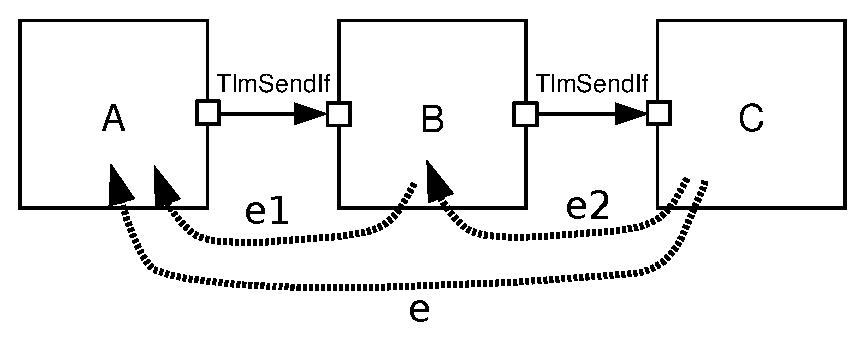
\includegraphics[width=10.0cm]{tlm/chaining_communication_steps.pdf}
    \caption{\label{fig:chaining_communication_steps} Chaining communication steps.}
  \end{center}
\end{figure}

\textbf{Chaining communication steps}. Most of the time a single event
is sufficient for a simple communication scheme. Sometimes several
communication steps are needed before the message actually reachs the
target. For instance, consider an intermediate module is placed
between the initiator and the target,
see~Figure~\ref{fig:chaining_communication_steps}.  Module~A is an
initiator. Module~B is both a target and an initiator. Module~C is a
target. The time spent in module~B affects the total transaction time
between initiator module~A and final target module~C. While the time
spent when processing the transition of the message from A-B to B-C
can be easily computed in module~B \texttt{Send} method, if a single
event is used, the computation of the time spent when the response
goes through B can not be computed, because the response will be
directly notified from module~C to module~A. To account for this
additional delay, only one event is not sufficient. Actually, an
additional event is needed to make module~B wait module~C, while
module~A still waits the target module, which is module~B not
module~C. A stack of events has been introduced to simplify the
programming of chained communication steps. Such communication schemes
are quite common in networks, where intermediate modules would be
switches. Before sending a message, an initiator puts both the request
and the event into the message. Actually, the event is pushed on a
stack. After the \texttt{Send}, the initiator still waits for the
event it has pushed on the stack. Once the event is notified, the
initiator is unblocked and can do a pop on the stack to remove its
event. The TLM interface has been updated to add support for an event
stack, see~Figure~\ref{fig:interface3} (note that access methods to
the stack of events have been omitted from the Figure).

\begin{figure}[h]
  \begin{center}
    \input{tlm/interface3}
    \caption{\label{fig:interface3} TLM interface (with an event stack).}
  \end{center}
\end{figure}

\section{Untimed TLM}
\label{sec:untimed_tlm}

\begin{figure}[h]
  \begin{center}
    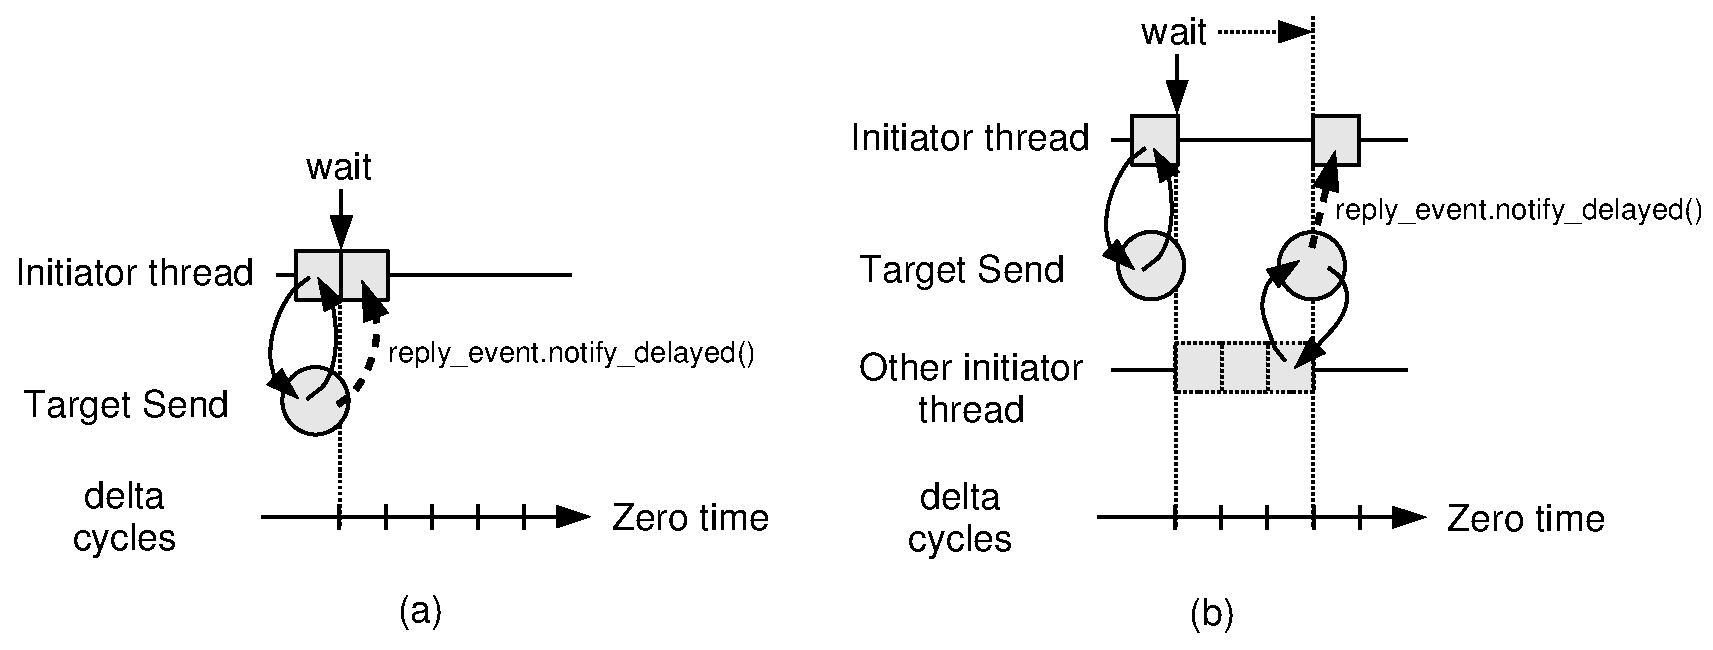
\includegraphics[width=\textwidth]{tlm/utlm_principle.pdf}
    \caption{\label{fig:utlm_principle} Untimed TLM: principle.}
  \end{center}
\end{figure}

This section will demonstrate the use of the TLM interface and message
to design untimed TLM models. In an Untimed TLM (UTLM) model, the
delays for serving requests is not considered,
see~Figure~\ref{fig:utlm_principle}. The simulated time is stuck to
zero and only delta cycles occur during simulation. The initiator
calls target method \texttt{Send} to make the target serve the
request. If the initiator waits for a response, i.e. waits for the
response event, the target triggers the response event for the next
delta cycle, see Figure~\ref{fig:utlm_principle}~(a). While making the initiator wait the response
  event may seem not necessary for untimed models, actually it is necessary
  because the target method \texttt{Send} may not trigger the response
  event before leaving control to the caller initiator thread
  but in another delta cycle. For example, the target may need to receive a
  message from another module to set the response and trigger the
  response event, see Figure~\ref{fig:utlm_principle}~(b).
  As a side effect, forcing this design methodology facilitates the untimed
  and timed models cosimulation, and enables a smooth transition from untimed models to
  timed models.

Consider the example of a system
with one processor and one memory: the processor is an initiator
whereas the memory is a target. Examples of request and response are
provided on Figure~\ref{fig:memory_req_rsp}. The processor can send
\texttt{READ} or \texttt{WRITE} requests to the memory. When the
request is a write, \texttt{MemoryRequest} member \texttt{write\_data}
helds the data to write.

\begin{figure}[p]
\begin{minipage}{\textwidth}
  \begin{center}
    \input{tlm/memory_req_rsp}
    \caption{\label{fig:memory_req_rsp} Example of memory request \& response.}
  \end{center}
\end{minipage}
\begin{minipage}{\textwidth}
~\vspace{3.0cm}
\end{minipage}
\begin{minipage}{\textwidth}
  \begin{center}
    \input{tlm/utlm_memory}
    \caption{\label{fig:utlm_memory} Example of UTLM memory module.}
  \end{center}
\end{minipage}
\end{figure}

A source code example for the processor is provided on
Figure~\ref{fig:utlm_processor}. The processor module has only one
SystemC thread: \texttt{Run}. Thread \texttt{Run} calls
\texttt{PerformRead} and \texttt{PerformWrite} member methods. These
two methods do memory requests using SystemC port \texttt{port}. The
\texttt{PerformRead} operation is the following:

\begin{enumerate}
\item[{\large \ding{202}}] a memory request is allocated;
\item[{\large \ding{203}}] a message is allocated, and initialized
  with the request and the response event;
\item[{\large \ding{204}}] the request is filled;
\item[{\large \ding{205}}] the message is sent using port method
  \texttt{Send}; \texttt{Send} is retried until it has
  succeeded;
\item[{\large \ding{206}}] if \texttt{Send} has failed, the processor
  waits for one delta cycle before actually retrying \texttt{Send};
\item[{\large \ding{207}}] once \texttt{Send} has succeeded, the
  processor waits for the response event;
\item[{\large \ding{208}}] once \texttt{wait} is finished, the
  processor can use the response.
\end{enumerate}

The \texttt{PerformWrite} operation is the following:
\begin{enumerate}
\item[{\large \ding{202}}] a memory request is allocated;
\item[{\large \ding{203}}] a message is allocated, and initialized
  with the request and the response event;
\item[{\large \ding{204}}] the request is filled;
\item[{\large \ding{205}}] the message is sent using port
  \texttt{Send} methods; \texttt{Send} is retried until it has
  succeeded;
\item[{\large \ding{206}}] if \texttt{Send} has failed, the processor
  waits for one delta cycle before actually retrying \texttt{Send};
\end{enumerate}

When \texttt{Send} fails and the processor has to wait for a delta
cycle before retrying (see item {\large \ding{206}} from the previous
operations), the programmer should use a private event to first notify
using \texttt{notify\_delayed} SystemC method and after that, perform
the \texttt{wait}, which effectively provoques a one delta cycle wait.
% We will see later, that \texttt{notify\_delayed} is only necessary
% when writing UTLM models, but not necessary for TTLM models.

\begin{figure}[p]
  \begin{center}
    \input{tlm/utlm_processor}
    \caption{\label{fig:utlm_processor} Example of UTLM processor
      module.}
  \end{center}
\end{figure}

A source code example for the memory is provided on
Figure~\ref{fig:utlm_memory}. The memory module has no thread. The
memory requests are directly served by memory method \texttt{Send}
within the processor module thread. Member method \texttt{Send}
operation is the following:

\begin{enumerate}
\item[{\large \ding{202}}] the request is taken from the message;
\item[{\large \ding{203}}] the response is allocated;
\item[{\large \ding{204}}] if the request is a \texttt{READ}, the
  reponse is filled with the read data; the response is put in the
  message and the response event is notified for the next delta cycle;
\item[{\large \ding{205}}] if the request is a \texttt{WRITE}, the
  data to write is written back in the memory.
\end{enumerate}


\section{Timed TLM}
\label{sec:timed_tlm}

\begin{figure}[h]
  \begin{center}
    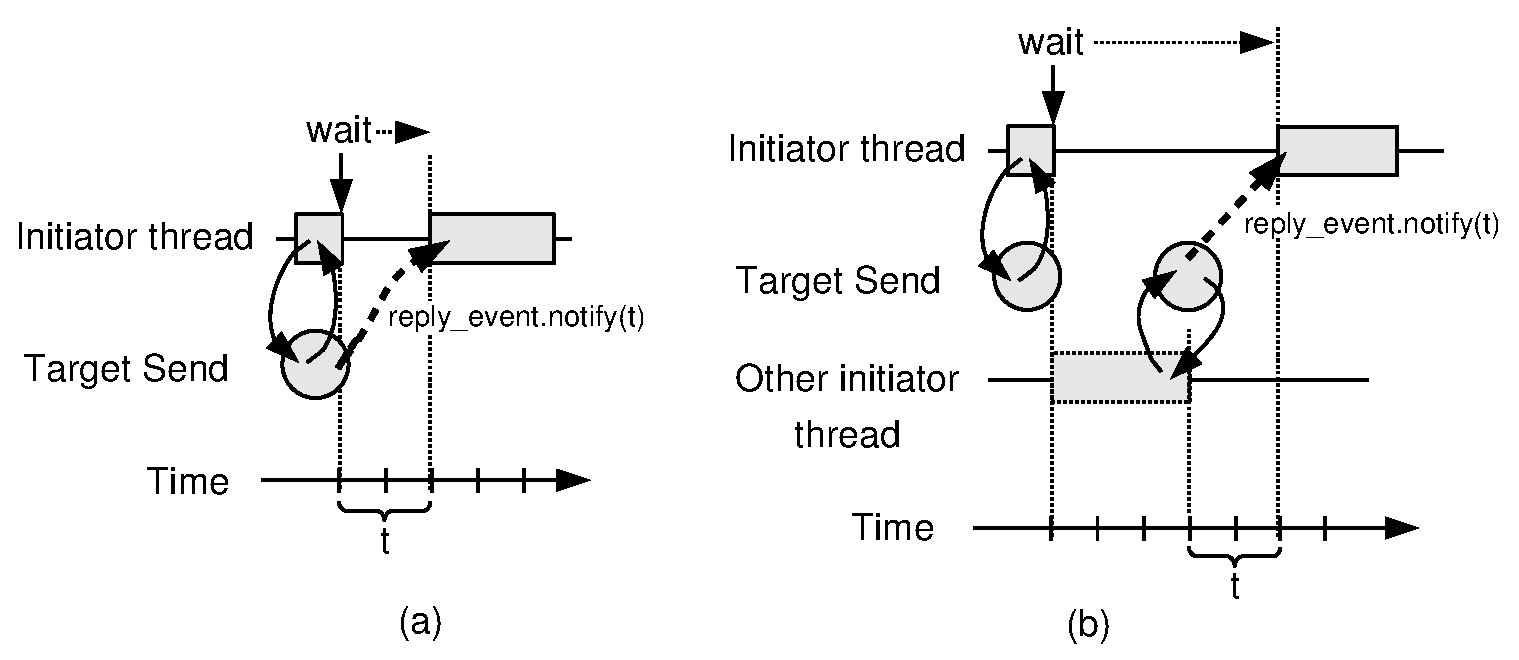
\includegraphics[width=\textwidth]{tlm/ttlm_principle.pdf}
    \caption{\label{fig:ttlm_principle} Timed TLM: principle.}
  \end{center}
\end{figure}

In this section, the use of the TLM interface and message with time
(TTLM) will be demonstrated on several examples with an increasing
complexity. The first example presents how to add time to the untimed
model using one-to-one communication scheme, see
section~\ref{sec:untimed_tlm}. The next example presents a N-to-M
communication scheme using a router between the processors and the
memory, and applying contention over the processors requests. The last
example presents an N-to-M communication scheme using a router between
the processors and the memories, and applying contention over
processors requests and memories responses. As several
processors/memories compete for accessing to the router, the router is
using an arbitration algorithm.  The arbitration algorithm assigns a
fixed time slot to each processor/memory.

In the proposed model the initiator must place itself in the right
time when sending a request, i.e., calling the \texttt{Send} method.
For that purpose, the initiator must use the \texttt{wait} method.
When the target needs to reply to a request the \texttt{notify} method
is used over the response event with the estimated time taken by the
target, see Figure~\ref{fig:ttlm_principle}. The target module
  can trigger the response event when executing the \texttt{Send}
  method, i.e., in the initiator thread, see
  Figure~\ref{fig:ttlm_principle}~(a); or during another cycle (or
  delta cycle), for example, the target module may need that another
  initiator module sends a message to it before triggering the first
  initiator response event, see Figure~\ref{fig:ttlm_principle}~(b).
Note that unlike in the UTLM model \texttt{notify\_delayed} is no
longer needed, unless the notification takes zero time.

\subsection{Example: Simple Model}
The modifications to the UTLM example to make it TTLM are minimal.
Processor and memory now have time parameters among their template
parameters (i.e., \texttt{FREQUENCY} and \texttt{READ\_CYCLES}), which
are used to compute the processor and memory processing times.

The main modification in the processor module is the substitution and
addition of calls to the SystemC primitive \texttt{wait} with time,
see {\large \ding{202}} and {\large \ding{203}} on
Figure~\ref{fig:ttlm_processor}\footnote{This implementation is
  innefficient, because a call to the \texttt{wait} method is done
  (that is, a SystemC synchronization) for each executed instruction.
  Better implementations can be done, but this is not the objective of
  this example.}. For example, it is used when trying to send a
read/write request, and the request fails, see {\large \ding{202}} on
Figure~\ref{fig:ttlm_processor}.  Another use is to advance the
internal clock of the module after an instruction execution, see
{\large \ding{203}} on Figure~\ref{fig:ttlm_processor}.

To convert the memory module to a TTLM module, we have only modified
the call to the \texttt{notify} method, see {\large \ding{202}} on
Figure~\ref{fig:ttlm_memory}, to indicate the time the memory needs to
set the response, the response delay time. Note that the memory sets
the response before notifying it, and that the response could be used
before the delay time, however the module that receives the response
should never suppose so, i.e., another implementation of the memory
could have wait the delay time before setting the response and simply
make a \texttt{notify\_delayed} to make it available.

\begin{figure}[p]
  \begin{center}
    \input{tlm/ttlm_processor}
    \caption{\label{fig:ttlm_processor} Example of TTLM processor.}
  \end{center}
\end{figure}

\begin{figure}[p]
\begin{minipage}{\textwidth}
  \begin{center}
    \input{tlm/ttlm_memory}
    \caption{\label{fig:ttlm_memory} Example of TTLM memory.}
  \end{center}
\end{minipage}
\begin{minipage}{\textwidth}
~\vspace{2.5cm}
\end{minipage}
\begin{minipage}{\textwidth}
  \begin{center}
    \input{tlm/ttlm_router}
    \caption{\label{fig:ttlm_router} Untimed implementation of the
      \texttt{router} module.}
  \end{center}
\end{minipage}
\end{figure}


\subsection{Example: Request contention}
\label{subsec:example_request_contention}

\begin{figure}[h]
  \begin{center}
    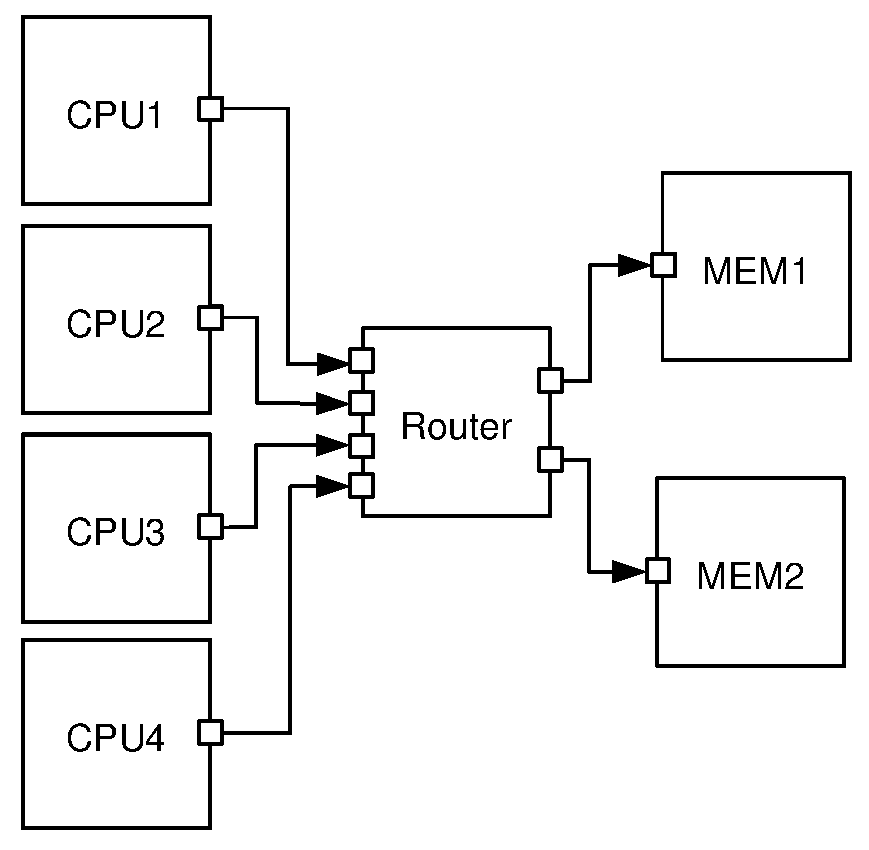
\includegraphics[width=7.0cm]{tlm/n_to_m.pdf}
    \caption{\label{fig:n_to_n} M-initiators~x~N-targets.}
  \end{center}
\end{figure}

This example shows how a module can perform contention over the
request. For that purpose a new module is added: the \texttt{router}
module which connects the processors to multiple memories, see
Figure~\ref{fig:n_to_n}. For a simple untimed implementation of the
\texttt{router} module see Figure~\ref{fig:ttlm_router}. This
implementation does not make any contention over the incomming
requests, neither over responses. This example is going to show how to
implement contention over the incomming requests, later
Section~\ref{subsec:example_response_contention} will show how to
implement contention over the responses.

The \texttt{router} module implements a round robin scheduling
algorithm to give access to the memories, i.e., if two processors are
simulated processor 0 has access to the memories during cycles 0, 2,
4,\ldots , and processor 1 at cycles 1, 3, 5,\ldots.
Figure~\ref{fig:ttlm_router_adv} shows a possible implementation. In
this implementation, the \texttt{router} module is a hierarchical
module that associates to each input port a \texttt{MasterPortModule}
module which actually implements the contention, see {\large
  \ding{202}} on Figure~\ref{fig:ttlm_router_adv}.

\texttt{MasterPortModule} bufferizes all the incomming requests and
dispatches them in the incomming order during the time windows
associated to the port using a thread. This module implements the
\texttt{Send} method from the \texttt{TlmSendIf} interface to handle
incomming requests, see {\large \ding{202}} and {\large \ding{203}} on
Figure~\ref{fig:ttlm_router_adv}. A buffer holds incomming requests
and the \texttt{Dispatch} thread of the module dispatches them to the
right output port during the time windows of the incomming port, see
{\large \ding{204}} on Figure~\ref{fig:ttlm_router_adv}.  To execute
the \texttt{Dispatch} process at the right time windows the
\texttt{dispatch\_event} (from which the \texttt{Dispatch} process
depends) has to be carefully triggered. In this example, the
\texttt{dispatch\_event} is triggered with the right delay when a new
request is queued (note that time can be equal to zero, which means
that the event will be notified during the next delta cycle, but the
SystemC clock will not be modified), see {\large \ding{205}} on
Figure~\ref{fig:ttlm_router_adv}. In case the buffer is not empty
after dispatching the oldest request (or if the oldest request has not
been accepted) another \texttt{dispatch\_event} is triggered, to
execute the \texttt{Dispatch} thread during the next time window and
send pending requests, see {\large \ding{206}} on
Figure~\ref{fig:ttlm_router_adv}.


\subsection{Example: Response contention}
\label{subsec:example_response_contention}
Section~\ref{subsec:example_request_contention} showed how contention
can be done over incomming requests. However, in many situations
contention over the responses is also desired. This example, modifies
the previously shown \texttt{router} with requests contention to
support contention over responses. For the new implementation of the
\texttt{router} see Figure~\ref{fig:ttlm_router_adv2}.

The \hfill hierarchical \hfill \texttt{router} \hfill module \hfill contains \hfill the \hfill definition \hfill of \hfill an \hfill additional \hfill module: the \texttt{SlavePortController} module, see
{\large \ding{202}} on Figure~\ref{fig:ttlm_router_adv2}. An instance
of this module is associated to each output port, and connected to
each of the instances of \texttt{MasterPortController}.

To easily handle multiple responses it implements the
\texttt{ResponseReceived} method from the \texttt{ResponseListener}
utility class (included in the source distribution of the TLM model
presented in this document), see {\large \ding{203}} and {\large
  \ding{204}} on Figure~\ref{fig:ttlm_router_adv2}.  Conceptually, the
\texttt{ResponseListener} utility class allows to send a message
through a port with the \texttt{Send} method provided by this class,
and be notified when the response is received thanks to the
\texttt{ResponseReceived} method.

The \texttt{SlavePortController} also implements the \texttt{Send}
method from the \texttt{TlmSendIf} interface to handle requests
comming from the \texttt{MasterPortController} modules, see {\large
  \ding{203}} and {\large \ding{205}} on
Figure~\ref{fig:ttlm_router_adv2}. The \texttt{Send} method checks if
the request requires a response:
\begin{itemize}
\item if not it just forwards the request to the output port, see
  {\large \ding{206}} on Figure~\ref{fig:ttlm_router_adv2};
\item if a response is required then it uses the \texttt{Send} method
  provided by the \texttt{ResponseListener} class to forward send the
  request through the output port, and be notified (through the
  \texttt{ResponseReceived} method when the response is available, see
  {\large \ding{207}} on Figure~\ref{fig:ttlm_router_adv2}.
\end{itemize}

When a response to a message is received the
\texttt{SlavePortController} handles it as the
\texttt{MasterPortController}, that is, it puts the message in a
buffer and dispatches it with the \texttt{Dispatch} thread during the
time windows given to the port, see {\large \ding{208}} on
Figure~\ref{fig:ttlm_router_adv2}.

\begin{figure}[p]
  \begin{center}
    \input{tlm/ttlm_router_adv}
    \caption{\label{fig:ttlm_router_adv} Example of TTLM router module
      with requests contention.}
  \end{center}
\end{figure}

\begin{figure}[p]
  \begin{center}
    \input{tlm/ttlm_router_adv2}
    \caption{\label{fig:ttlm_router_adv2} Example of TTLM router
      module with requests and responses contention.}
  \end{center}
\end{figure}


\chapter{Services}
\label{services}
Designing a new emulator, and particularly for a research purpose, means implementing an instruction set emulator but also involves several software components not directly related to pure instruction set execution.
The most obvious needed software components are memories, debuggers, loaders, but components such as chipsets and peripherals are still mandatory to enable running real unmodified applications.
Making all these components running together requires programming interfaces as much standard as possible.

Usually the programmer faces to the problems of sharing source codes among several emulators, reusing existing source codes, and building a fully functional emulator from all these heterogeneous pieces of source codes.
Most of the time, the software components are strongly dependent for each other: components are statically linked together through explicit function calls and adhoc interfaces.
Replacing these adhoc interfaces with C++ pure interfaces (C++ classes with only unimplemented virtual methods, see your C++ manual for more details) and linking the components through pointers is a step toward avoiding such strong dependencies between the components. But still finding a standard manner to initialize those pointers is necessary. This can be done either by directly writting in those pointers or calling special functions to do the job.

Another problem with heterogeneous software components is the manner to instantiate and parameterize those components in a standard way, so that it is easier for the component's user to use a new component.
Usually, parameterizing a component means passing arguments to an initialization function or a class constructor. It implies that the programmers agree on using only one of these two solutions or both.
Still the programmers must know the setup order of these components: it is an error prone process because determining a correct order from the components documentation will likely fail the first times.

% problems:\\
% - C++ class code sharing/reuse/composition\\
% - direct call problem\\
% - parameterization problem\\
% - setup problem: dependencies, which setup order ?\\
% \\

In this section, we propose a standard way to share, reuse, link, parameterize and setup these software components.
C++ object oriented programming and pure C++ interfaces enable sharing and reuse.
Some special pointers (classes \texttt{ServiceImport} and \texttt{ServiceExport}) linking the software components (classes \texttt{Service} and \texttt{Client}) together with some base software component classes have been introduced, thus enabling easier component composition and connection.
The parameterization have been standardized (class \texttt{Parameter}) and the framework (class \texttt{ServiceManager}) uses the call graph to provide the user with an automatic setup order.

Section~\ref{services_library} documents the available services in the library. Section~\ref{building_a_service_graph} presents how to use services, link clients and services, and setup each components. Section~\ref{designing_clients_and_services} not only presents how to design a service, either a totally new service, or an assembly of existing services, but also how to design a client invoking a service.

% solution:\\
% sharing/reuse -> classes, abstract interfaces\\
% composition -> service, client, import/export, call/use graph (connections)\\
% parameterization -> generic parameters\\
% setup problem -> call/use graph enables automatic setup order\\

\section{Service Interfaces}
\label{service_interfaces}

\section{Services library}
\label{services_library}

% \newpage
% \begin{center}
% 	\begin{tabular}{|p{7.5cm}|p{7.5cm}|}
% 		\hline
% 		\multicolumn{2}{|l|}{\textbf{\Large Service Sample}}\\
% 		\hline
% 		\multicolumn{1}{|p{7.5cm}}{\textbf{Class Name:} \newline \texttt{sample::sample::sample}\newline$\hookrightarrow$\texttt{::sample}} & \multicolumn{1}{p{7.5cm}|}{\textbf{Header:} \newline \texttt{sample/sample/sample}\newline$\hookrightarrow$\texttt{/sample.hh}}\\
% 		\multicolumn{2}{|l|}{}\\
% 		\multicolumn{2}{|p{15cm}|}{\textbf{Description:} \newline Sample.}\\
% 		\hline
% 		\hline
% 		\multicolumn{2}{|c|}{\textbf{\large Template Parameters}}\\
% 		\hline
% 		\multicolumn{1}{|p{7.5cm}}{\textbf{Name:} \texttt{sample}} & \multicolumn{1}{p{7.5cm}|}{\textbf{Type:} \texttt{sample}}\\
% 		\multicolumn{2}{|p{15cm}|}{\textbf{Default value:} \texttt{sample}}\\
% 		\multicolumn{2}{|l|}{}\\
% 		\multicolumn{2}{|p{15cm}|}{\textbf{Description:} \newline Sample.}\\
% 		\hline
% 		\hline
% 		\multicolumn{2}{|c|}{\textbf{\large Run-Time Parameters}}\\
% 		\hline
% 		\multicolumn{1}{|p{7.5cm}}{\textbf{Name:} \texttt{sample}} & \multicolumn{1}{p{7.5cm}|}{\textbf{Type:} \texttt{sample}}\\
% 		\multicolumn{2}{|p{15cm}|}{\textbf{Default value:} \texttt{sample}}\\
% 		\multicolumn{2}{|l|}{}\\
% 		\multicolumn{2}{|p{15cm}|}{\textbf{Description:} \newline Sample.}\\
% 		\hline
% 		\hline
% 		\multicolumn{2}{|c|}{\textbf{\large Service Exports}}\\
% 		\hline
% 		\multicolumn{1}{|p{7.5cm}}{\textbf{Name:} \texttt{sample}} & \multicolumn{1}{p{7.5cm}|}{\textbf{Interface:} \newline \texttt{sample} \newline$\hookrightarrow$\texttt{sample}}\\
% 		\multicolumn{2}{|l|}{}\\
% 		\multicolumn{2}{|p{15cm}|}{\textbf{Description:} \newline Sample.}\\
% 		\hline
% 		\hline
% 		\multicolumn{2}{|c|}{\textbf{\large Service Imports}}\\
% 		\hline
% 		\multicolumn{1}{|p{7.5cm}}{\textbf{Name:} \texttt{sample} \newline \textbf{Mandatory connected:} yes/no} & \multicolumn{1}{p{7.5cm}|}{\textbf{Interface:} \newline \texttt{sample::sample::sample} \newline$\hookrightarrow$\texttt{::sample}}\\
% 		\multicolumn{2}{|l|}{}\\
% 		\multicolumn{2}{|p{15cm}|}{\textbf{Description:} \newline Sample.}\\
% 		\hline
% 	\end{tabular}
% \end{center}

\subsection{Loaders}

\newpage
\begin{center}
	\begin{tabular}{|p{7.5cm}|p{7.5cm}|}
		\hline
		\multicolumn{2}{|l|}{\textbf{\Large Service ELF Loader}}\\
		\hline
		\multicolumn{1}{|p{7.5cm}}{\textbf{Class Name:} \newline \texttt{unisim::service::loader::elf\_loader}\newline$\hookrightarrow$\texttt{::ElfLoaderImpl}} & \multicolumn{1}{p{7.5cm}|}{\textbf{Header:} \newline \texttt{unisim/service/loader/elf\_loader}\newline$\hookrightarrow$\texttt{/elf\_loader.hh}}\\
		\multicolumn{2}{|l|}{}\\
		\multicolumn{2}{|p{15cm}|}{\textbf{Description:} \newline The ELF loader service allows to load a binary program into a memory and fill a symbol table.
		The loader also provides information about the loaded file such as the code and data locations (base address and size). The ELF loader loads the program during setup. \texttt{Elf32Loader} and \texttt{Elf64Loader} are two specialized versions of class \texttt{ElfLoaderImpl<>} which the user should use whenever possible.}\\
		\hline
		\hline
		\multicolumn{2}{|l|}{\textbf{Template Parameters}}\\
		\hline
		\multicolumn{1}{|p{7.5cm}}{\textbf{Name:} \texttt{MEMORY\_ADDR}} & \multicolumn{1}{p{7.5cm}|}{\textbf{Type:} \texttt{class}}\\
		\multicolumn{2}{|p{15cm}|}{\textbf{Default value:} none}\\
		\multicolumn{2}{|l|}{}\\
		\multicolumn{2}{|p{15cm}|}{\textbf{Description:} \newline This is the C++ type of a memory address (e.g. uint32\_t or uint64\_t).}\\
		\hline
		\multicolumn{1}{|p{7.5cm}}{\textbf{Name:} \texttt{T}} & \multicolumn{1}{p{7.5cm}|}{\textbf{Type:} \texttt{class}}\\
		\multicolumn{2}{|p{15cm}|}{\textbf{Default value:} none}\\
		\multicolumn{2}{|l|}{}\\
		\multicolumn{2}{|p{15cm}|}{\textbf{Description:} \newline We should consider removing this parameter or have a reason to have it.}\\
		\hline
		\multicolumn{1}{|p{7.5cm}}{\textbf{Name:} \texttt{ElfClass}} & \multicolumn{1}{p{7.5cm}|}{\textbf{Type:} \texttt{unsigned int}}\\
		\multicolumn{2}{|p{15cm}|}{\textbf{Default value:} none}\\
		\multicolumn{2}{|l|}{}\\
		\multicolumn{2}{|p{15cm}|}{\textbf{Description:} \newline class of machine (either \texttt{ELFCLASS32} or \texttt{ELFCLASS64}).}\\
		\hline
		\multicolumn{1}{|p{7.5cm}}{\textbf{Name:} \texttt{Elf\_Ehdr}} & \multicolumn{1}{p{7.5cm}|}{\textbf{Type:} \texttt{class}}\\
		\multicolumn{2}{|p{15cm}|}{\textbf{Default value:} none}\\
		\multicolumn{2}{|l|}{}\\
		\multicolumn{2}{|p{15cm}|}{\textbf{Description:} \newline ELF Header structure (either Elf32\_Ehdr or Elf64\_Ehdr).}\\
		\hline
		\multicolumn{1}{|p{7.5cm}}{\textbf{Name:} \texttt{Elf\_Phdr}} & \multicolumn{1}{p{7.5cm}|}{\textbf{Type:} \texttt{class}}\\
		\multicolumn{2}{|p{15cm}|}{\textbf{Default value:} none}\\
		\multicolumn{2}{|l|}{}\\
		\multicolumn{2}{|p{15cm}|}{\textbf{Description:} \newline ELF Program Header structure (either Elf32\_Phdr or Elf64\_Phdr).}\\
		\hline
		\multicolumn{1}{|p{7.5cm}}{\textbf{Name:} \texttt{Elf\_Shdr}} & \multicolumn{1}{p{7.5cm}|}{\textbf{Type:} \texttt{class}}\\
		\multicolumn{2}{|p{15cm}|}{\textbf{Default value:} none}\\
		\multicolumn{2}{|l|}{}\\
		\multicolumn{2}{|p{15cm}|}{\textbf{Description:} \newline ELF Section Header structure (either \texttt{Elf32\_Shdr} or \texttt{Elf64\_Shdr}).}\\
		\hline
		\multicolumn{1}{|p{7.5cm}}{\textbf{Name:} \texttt{Elf\_Sym}} & \multicolumn{1}{p{7.5cm}|}{\textbf{Type:} \texttt{class}}\\
		\multicolumn{2}{|p{15cm}|}{\textbf{Default value:} none}\\
		\multicolumn{2}{|l|}{}\\
		\multicolumn{2}{|p{15cm}|}{\textbf{Description:} \newline ELF Symbol structure (either \texttt{Elf32\_Sym} or \texttt{Elf64\_Sym}).}\\
		\hline
	\end{tabular}
\end{center}

\begin{center}
	\begin{tabular}{|p{7.5cm}|p{7.5cm}|}
		\hline
		\multicolumn{2}{|c|}{\textbf{\large Run-Time Parameters}}\\
		\hline
		\multicolumn{1}{|p{7.5cm}}{\textbf{Name:} \texttt{filename}} & \multicolumn{1}{p{7.5cm}|}{\textbf{Type:} \texttt{string}}\\
		\multicolumn{2}{|p{15cm}|}{\textbf{Default value:} empty string}\\
		\multicolumn{2}{|l|}{}\\
		\multicolumn{2}{|p{15cm}|}{\textbf{Description:} \newline The ELF file name to load into the connected memory.}\\
		\hline
		\multicolumn{1}{|p{7.5cm}}{\textbf{Name:} \texttt{base-addr}} & \multicolumn{1}{p{7.5cm}|}{\textbf{Type:} \texttt{MEMORY\_ADDR}}\\
		\multicolumn{2}{|p{15cm}|}{\textbf{Default value:} \texttt{0}}\\
		\multicolumn{2}{|l|}{}\\
		\multicolumn{2}{|p{15cm}|}{\textbf{Description:} \newline If this parameter is non-zero, force the ELF Loader to load the unique program segment at this base address.}\\
		\hline
		\multicolumn{1}{|p{7.5cm}}{\textbf{Name:} \texttt{force-use-virtual-address}} & \multicolumn{1}{p{7.5cm}|}{\textbf{Type:} \texttt{bool}}\\
		\multicolumn{2}{|p{15cm}|}{\textbf{Default value:} \texttt{false}}\\
		\multicolumn{2}{|l|}{}\\
		\multicolumn{2}{|p{15cm}|}{\textbf{Description:} \newline If true, this parameter forces the ELF loader to use the segment virtual address instead of the segment physical address when loading the segments into memory.}\\
		\hline
		\hline
		\multicolumn{2}{|c|}{\textbf{\large Service Exports}}\\
		\hline
		\multicolumn{1}{|p{7.5cm}}{\textbf{Name:} \texttt{logger\_export}} & \multicolumn{1}{p{7.5cm}|}{\textbf{Interface:} \newline \texttt{unisim::service::interfaces::} \newline$\hookrightarrow$\texttt{Loader<MEMORY\_ADDR>}}\\
		\multicolumn{2}{|l|}{}\\
		\multicolumn{2}{|p{15cm}|}{\textbf{Description:} \newline The ELF loader provides information about the code and data location through this export.}\\
		\hline
		\hline
		\multicolumn{2}{|c|}{\textbf{\large Service Imports}}\\
		\hline
		\multicolumn{1}{|p{7.5cm}}{\textbf{Name:} \texttt{memory\_import}} & \multicolumn{1}{p{7.5cm}|}{\textbf{Interface:} \newline \texttt{unisim::service::interfaces::} \newline$\hookrightarrow$\texttt{Memory<MEMORY\_ADDR>}}\\
		\multicolumn{2}{|p{15cm}|}{\textbf{Mandatory connected:} no}\\
		\multicolumn{2}{|l|}{}\\
		\multicolumn{2}{|p{15cm}|}{\textbf{Description:} \newline The ELF loader accesses to the memory through this import.}\\
		\hline
		\multicolumn{1}{|p{7.5cm}}{\textbf{Name:} \texttt{symbol\_table\_build\_import}} & \multicolumn{1}{p{7.5cm}|}{\textbf{Interface:} \newline \texttt{unisim::service::interfaces::} \newline$\hookrightarrow$\texttt{SymbolTableBuild<MEMORY\_ADDR>}}\\
		\multicolumn{2}{|p{15cm}|}{\textbf{Mandatory connected:} no}\\
		\multicolumn{2}{|l|}{}\\
		\multicolumn{2}{|p{15cm}|}{\textbf{Description:} \newline The ELF loader fills the symbol table using this import.}\\
		\hline
	\end{tabular}
\end{center}

\newpage
\begin{center}
	\begin{tabular}{|p{7.5cm}|p{7.5cm}|}
		\hline
		\multicolumn{2}{|l|}{\textbf{\Large Service ELF32 Loader}}\\
		\hline
		\multicolumn{1}{|p{7.5cm}}{\textbf{Class Name:} \newline \texttt{unisim::service::loader::elf\_loader}\newline$\hookrightarrow$\texttt{::Elf32Loader}} & \multicolumn{1}{p{7.5cm}|}{\textbf{Header:} \newline \texttt{unisim/service/loader/elf\_loader}\newline$\hookrightarrow$\texttt{/elf\_loader.hh}}\\
		\multicolumn{2}{|l|}{}\\
		\multicolumn{2}{|p{15cm}|}{\textbf{Description:} \newline The ELF32 loader service allows to load an ELF32 binary program into a memory and fill a symbol table. The loader also provides information about the loaded file such as the code and data locations (base address and size). The ELF loader loads the program during setup.}\\
		\hline
		\hline
		\multicolumn{2}{|c|}{\textbf{\large Run-Time Parameters}}\\
		\hline
		\multicolumn{1}{|p{7.5cm}}{\textbf{Name:} \texttt{filename}} & \multicolumn{1}{p{7.5cm}|}{\textbf{Type:} \texttt{string}}\\
		\multicolumn{2}{|p{15cm}|}{\textbf{Default value:} empty string}\\
		\multicolumn{2}{|l|}{}\\
		\multicolumn{2}{|p{15cm}|}{\textbf{Description:} \newline The ELF file name to load into the connected memory.}\\
		\hline
		\multicolumn{1}{|p{7.5cm}}{\textbf{Name:} \texttt{base-addr}} & \multicolumn{1}{p{7.5cm}|}{\textbf{Type:} \texttt{uint32\_t}}\\
		\multicolumn{2}{|p{15cm}|}{\textbf{Default value:} \texttt{0}}\\
		\multicolumn{2}{|l|}{}\\
		\multicolumn{2}{|p{15cm}|}{\textbf{Description:} \newline If this parameter is non-zero, force the ELF Loader to load the unique program segment at this base address.}\\
		\hline
		\multicolumn{1}{|p{7.5cm}}{\textbf{Name:} \texttt{force-use-virtual-address}} & \multicolumn{1}{p{7.5cm}|}{\textbf{Type:} \texttt{bool}}\\
		\multicolumn{2}{|p{15cm}|}{\textbf{Default value:} \texttt{false}}\\
		\multicolumn{2}{|l|}{}\\
		\multicolumn{2}{|p{15cm}|}{\textbf{Description:} \newline If true, this parameter forces the ELF loader to use the segment virtual address instead of the segment physical address when loading the segments into memory.}\\
		\hline
		\hline
		\multicolumn{2}{|c|}{\textbf{\large Service Exports}}\\
		\hline
		\multicolumn{1}{|p{7.5cm}}{\textbf{Name:} \texttt{logger\_export}} & \multicolumn{1}{p{7.5cm}|}{\textbf{Interface:} \newline \texttt{unisim::service::interfaces::} \newline$\hookrightarrow$\texttt{Loader<uint32\_t>}}\\
		\multicolumn{2}{|l|}{}\\
		\multicolumn{2}{|p{15cm}|}{\textbf{Description:} \newline The ELF loader provides information about the code and data location through this export.}\\
		\hline
		\hline
		\multicolumn{2}{|c|}{\textbf{\large Service Imports}}\\
		\hline
		\multicolumn{1}{|p{7.5cm}}{\textbf{Name:} \texttt{memory\_import} \newline \textbf{Mandatory connected:} no} & \multicolumn{1}{p{7.5cm}|}{\textbf{Interface:} \newline \texttt{unisim::service::interfaces::} \newline$\hookrightarrow$\texttt{Memory<uint32\_t>}}\\
		\multicolumn{2}{|l|}{}\\
		\multicolumn{2}{|p{15cm}|}{\textbf{Description:} \newline The ELF loader accesses to the memory through this import.}\\
		\hline
		\multicolumn{1}{|p{7.5cm}}{\textbf{Name:} \texttt{symbol\_table\_build\_import} \newline \textbf{Mandatory connected:} no} & \multicolumn{1}{p{7.5cm}|}{\textbf{Interface:} \newline \texttt{unisim::service::interfaces::} \newline$\hookrightarrow$\texttt{SymbolTableBuild<uint32\_t>}}\\
		\multicolumn{2}{|l|}{}\\
		\multicolumn{2}{|p{15cm}|}{\textbf{Description:} \newline The ELF loader fills the symbol table using this import.}\\
		\hline
	\end{tabular}
\end{center}

\newpage
\begin{center}
	\begin{tabular}{|p{7.5cm}|p{7.5cm}|}
		\hline
		\multicolumn{2}{|l|}{\textbf{\Large Service ELF64 Loader}}\\
		\hline
		\multicolumn{1}{|p{7.5cm}}{\textbf{Class Name:} \newline \texttt{unisim::service::loader::elf\_loader}\newline$\hookrightarrow$\texttt{::Elf32Loader}} & \multicolumn{1}{p{7.5cm}|}{\textbf{Header:} \newline \texttt{unisim/service/loader/elf\_loader}\newline$\hookrightarrow$\texttt{/elf\_loader.hh}}\\
		\multicolumn{2}{|l|}{}\\
		\multicolumn{2}{|p{15cm}|}{\textbf{Description:} \newline The ELF32 loader service allows to load an ELF64 binary program into a memory and fill a symbol table. The loader also provides information about the loaded file such as the code and data locations (base address and size). The ELF loader loads the program during setup.}\\
		\hline
		\hline
		\multicolumn{2}{|c|}{\textbf{\large Run-Time Parameters}}\\
		\hline
		\multicolumn{1}{|p{7.5cm}}{\textbf{Name:} \texttt{filename}} & \multicolumn{1}{p{7.5cm}|}{\textbf{Type:} \texttt{string}}\\
		\multicolumn{2}{|p{15cm}|}{\textbf{Default value:} empty string}\\
		\multicolumn{2}{|l|}{}\\
		\multicolumn{2}{|p{15cm}|}{\textbf{Description:} \newline The ELF file name to load into the connected memory.}\\
		\hline
		\multicolumn{1}{|p{7.5cm}}{\textbf{Name:} \texttt{base-addr}} & \multicolumn{1}{p{7.5cm}|}{\textbf{Type:} \texttt{uint64\_t}}\\
		\multicolumn{2}{|p{15cm}|}{\textbf{Default value:} \texttt{0}}\\
		\multicolumn{2}{|l|}{}\\
		\multicolumn{2}{|p{15cm}|}{\textbf{Description:} \newline If this parameter is non-zero, force the ELF Loader to load the unique program segment at this base address.}\\
		\hline
		\multicolumn{1}{|p{7.5cm}}{\textbf{Name:} \texttt{force-use-virtual-address}} & \multicolumn{1}{p{7.5cm}|}{\textbf{Type:} \texttt{bool}}\\
		\multicolumn{2}{|p{15cm}|}{\textbf{Default value:} \texttt{false}}\\
		\multicolumn{2}{|l|}{}\\
		\multicolumn{2}{|p{15cm}|}{\textbf{Description:} \newline If true, this parameter forces the ELF loader to use the segment virtual address instead of the segment physical address when loading the segments into memory.}\\
		\hline
		\hline
		\multicolumn{2}{|c|}{\textbf{\large Service Exports}}\\
		\hline
		\multicolumn{1}{|p{7.5cm}}{\textbf{Name:} \texttt{logger\_export}} & \multicolumn{1}{p{7.5cm}|}{\textbf{Interface:} \newline \texttt{unisim::service::interfaces::} \newline$\hookrightarrow$\texttt{Loader<uint64\_t>}}\\
		\multicolumn{2}{|l|}{}\\
		\multicolumn{2}{|p{15cm}|}{\textbf{Description:} \newline The ELF loader provides information about the code and data location through this export.}\\
		\hline
		\hline
		\multicolumn{2}{|c|}{\textbf{\large Service Imports}}\\
		\hline
		\multicolumn{1}{|p{7.5cm}}{\textbf{Name:} \texttt{memory\_import} \newline \textbf{Mandatory connected:} no} & \multicolumn{1}{p{7.5cm}|}{\textbf{Interface:} \newline \texttt{unisim::service::interfaces::} \newline$\hookrightarrow$\texttt{Memory<uint64\_t>}}\\
		\multicolumn{2}{|l|}{}\\
		\multicolumn{2}{|p{15cm}|}{\textbf{Description:} \newline The ELF loader accesses to the memory through this import.}\\
		\hline
		\multicolumn{1}{|p{7.5cm}}{\textbf{Name:} \texttt{symbol\_table\_build\_import} \newline \textbf{Mandatory connected:} no} & \multicolumn{1}{p{7.5cm}|}{\textbf{Interface:} \newline \texttt{unisim::service::interfaces::} \newline$\hookrightarrow$\texttt{SymbolTableBuild<uint64\_t>}}\\
		\multicolumn{2}{|l|}{}\\
		\multicolumn{2}{|p{15cm}|}{\textbf{Description:} \newline The ELF loader fills the symbol table using this import.}\\
		\hline
	\end{tabular}
\end{center}


% \subsubsection{PowerMac BootX Loader}
% 
% \subsubsection{PowerMAC Linux Kernel Loader}
% 
% \subsubsection{S19 Loader}

\subsection{Operating System Application Binary Interface (OS ABI)}

\subsubsection{Linux OS system call translator}

\subsection{Debug}

\newpage
\begin{center}
	\begin{tabular}{|p{7.5cm}|p{7.5cm}|}
		\hline
		\multicolumn{2}{|l|}{\textbf{\Large Service Inline Debugger}}\\
		\hline
		\multicolumn{1}{|p{7.5cm}}{\textbf{Class Name:} \newline \texttt{unisim::service::debug}\newline$\hookrightarrow$\texttt{::inline\_debugger::InlineDebugger}} & \multicolumn{1}{p{7.5cm}|}{\textbf{Header:} \newline \texttt{unisim/service/debug}\newline$\hookrightarrow$\texttt{/inline\_debugger/inline\_debugger.hh}}\\
		\multicolumn{2}{|l|}{}\\
		\multicolumn{2}{|p{15cm}|}{\textbf{Description:} \newline The inline debugger service allows the user to interactively debug a target application running on a CPU module. The debug is at the instruction level. The inline debugger may be connected to a CPU module and (optionally) to a symbol table.}\\
		\hline
		\hline
		\multicolumn{2}{|c|}{\textbf{\large Template Parameters}}\\
		\hline
		\multicolumn{1}{|p{7.5cm}}{\textbf{Name:} \texttt{ADDRESS}} & \multicolumn{1}{p{7.5cm}|}{\textbf{Type:} \texttt{class}}\\
		\multicolumn{2}{|p{15cm}|}{\textbf{Default value:} none}\\
		\multicolumn{2}{|l|}{}\\
		\multicolumn{2}{|p{15cm}|}{\textbf{Description:} \newline This is the C++ type of a memory address (e.g. uint32\_t or uint64\_t).}\\
		\hline
		\hline
		\multicolumn{2}{|c|}{\textbf{\large Service Exports}}\\
		\hline
		\multicolumn{1}{|p{7.5cm}}{\textbf{Name:} \texttt{debug\_control\_export}} & \multicolumn{1}{p{7.5cm}|}{\textbf{Interface:} \newline \texttt{unisim::service::interfaces} \newline$\hookrightarrow$\texttt{::DebugControl<ADDRESS>}}\\
		\multicolumn{2}{|l|}{}\\
		\multicolumn{2}{|p{15cm}|}{\textbf{Description:} \newline This service export should be connected to a CPU module. The CPU module calls method \texttt{FetchDebugCommand} through its service import to leave control to the debugger and fetch a new debug command.}\\
		\hline
		\multicolumn{1}{|p{7.5cm}}{\textbf{Name:} \texttt{memory\_access\_reporting\_export}} & \multicolumn{1}{p{7.5cm}|}{\textbf{Interface:} \newline \texttt{unisim::service::interfaces} \newline$\hookrightarrow$\texttt{MemoryAccessReporting<ADDRESS>}}\\
		\multicolumn{2}{|l|}{}\\
		\multicolumn{2}{|p{15cm}|}{\textbf{Description:} \newline This service export should be connected to a CPU module. The CPU module calls methods \texttt{ReportMemoryAccess} and \texttt{ReportFinishedInstruction} through its service import. This allows the debugger to spy memory accesses and thus handle breakpoints and watchpoints.}\\
		\hline
		\multicolumn{1}{|p{7.5cm}}{\textbf{Name:} \texttt{trap\_reporting\_export}} & \multicolumn{1}{p{7.5cm}|}{\textbf{Interface:} \newline \texttt{unisim::service::interfaces} \newline$\hookrightarrow$\texttt{::TrapReporting}}\\
		\multicolumn{2}{|l|}{}\\
		\multicolumn{2}{|p{15cm}|}{\textbf{Description:} \newline This service export should be connected to a CPU module. A CPU module calls method \texttt{ReportTrap} through its service import. This allows the debugger to break execution on the simulated CPU once a trap condition is detected by the CPU module.}\\
		\hline
	\end{tabular}
\end{center}

\newpage
\begin{center}
	\begin{tabular}{|p{7.5cm}|p{7.5cm}|}
		\hline
		\multicolumn{2}{|c|}{\textbf{\large Service Imports}}\\
		\hline
		\multicolumn{1}{|p{7.5cm}}{\textbf{Name:} \texttt{disasm\_import} \newline \textbf{Mandatory connected:} yes} & \multicolumn{1}{p{7.5cm}|}{\textbf{Interface:} \newline \texttt{unisim::service::interfaces} \newline$\hookrightarrow$\texttt{::Disassembly<ADDRESS>}}\\
		\multicolumn{2}{|l|}{}\\
		\multicolumn{2}{|p{15cm}|}{\textbf{Description:} \newline This service import should be connected to a CPU module. The CPU module should implements method \texttt{Disassemble} which provides the debugger with disassembling of the instructions.}\\
		\hline
		\multicolumn{1}{|p{7.5cm}}{\textbf{Name:} \texttt{memory\_import} \newline \textbf{Mandatory connected:} yes} & \multicolumn{1}{p{7.5cm}|}{\textbf{Interface:} \newline \texttt{unisim::service::interfaces} \newline$\hookrightarrow$\texttt{::Memory<ADDRESS>}}\\
		\multicolumn{2}{|l|}{}\\
		\multicolumn{2}{|p{15cm}|}{\textbf{Description:} \newline This service import should be connected to a CPU or a memory module. The debugger uses this service import to access to memory using methods \texttt{ReadMemory} and \texttt{WriteMemory}.}\\
		\hline
		\multicolumn{1}{|p{7.5cm}}{\textbf{Name:} \texttt{memory\_access\_reporting\newline$\hookrightarrow$\_control\_import} \newline \textbf{Mandatory connected:} no} & \multicolumn{1}{p{7.5cm}|}{\textbf{Interface:} \newline \texttt{unisim::service::interfaces} \newline$\hookrightarrow$\texttt{::MemoryAccessReportingControl}}\\
		\multicolumn{2}{|l|}{}\\
		\multicolumn{2}{|p{15cm}|}{\textbf{Description:} \newline This service import should be connected to a CPU module. The debugger calls methods \texttt{RequiresMemoryAccessReporting} and \texttt{RequiresFinishedInstructionReporting} through this service import to enable/disable memory access reporting from the CPU module.}\\
		\hline
		\multicolumn{1}{|p{7.5cm}}{\textbf{Name:} \texttt{registers\_import} \newline \textbf{Mandatory connected:} yes} & \multicolumn{1}{p{7.5cm}|}{\textbf{Interface:} \newline \texttt{unisim::service::interfaces} \newline$\hookrightarrow$\texttt{::Registers}}\\
		\multicolumn{2}{|l|}{}\\
		\multicolumn{2}{|p{15cm}|}{\textbf{Description:} \newline This service import should be connected to a CPU module. The debugger calls method \texttt{GetRegister} through this service import to get an interface to the CPU registers. The debugger uses methods \texttt{GetName}, \texttt{GetValue}, \texttt{GetSize} and \texttt{SetValue} of that interface to access to CPU registers.}\\
		\hline
		\multicolumn{1}{|p{7.5cm}}{\textbf{Name:} \texttt{symbol\_table\_lookup\_import} \newline \textbf{Mandatory connected:} no} & \multicolumn{1}{p{7.5cm}|}{\textbf{Interface:} \newline \texttt{unisim::service::interfaces} \newline$\hookrightarrow$\texttt{::SymbolTableLookup}}\\
		\multicolumn{2}{|l|}{}\\
		\multicolumn{2}{|p{15cm}|}{\textbf{Description:} \newline This service import should be connected to a symbol table. The debugger calls method \texttt{FindSymbol}, \texttt{FindSymbolByAddr}, \texttt{FindSymbolByName} through this service import to translate address to symbol and vice-versa.}\\
		\hline
	\end{tabular}
\end{center}

\newpage
\begin{center}
	\begin{tabular}{|p{7.5cm}|p{7.5cm}|}
		\hline
		\multicolumn{2}{|l|}{\textbf{\Large Service GDB Server}}\\
		\hline
		\multicolumn{1}{|p{7.5cm}}{\textbf{Class Name:} \newline \texttt{unisim::service::debug}\newline$\hookrightarrow$\texttt{::gdb\_server::GDBServer}} & \multicolumn{1}{p{7.5cm}|}{\textbf{Header:} \newline \texttt{unisim/service/debug}\newline$\hookrightarrow$\texttt{/gdb\_server/gdb\_server.hh}}\\
		\multicolumn{2}{|l|}{}\\
		\multicolumn{2}{|p{15cm}|}{\textbf{Description:} \newline The GDB server service allows the user to interactively debug a target application running on a CPU module. The debug is at the instruction level and/or source level. The GDB server service may be connected to a CPU module.}\\
		\hline
		\hline
		\multicolumn{2}{|c|}{\textbf{\large Template Parameters}}\\
		\hline
		\multicolumn{1}{|p{7.5cm}}{\textbf{Name:} \texttt{ADDRESS}} & \multicolumn{1}{p{7.5cm}|}{\textbf{Type:} \texttt{class}}\\
		\multicolumn{2}{|p{15cm}|}{\textbf{Default value:} none}\\
		\multicolumn{2}{|l|}{}\\
		\multicolumn{2}{|p{15cm}|}{\textbf{Description:} \newline This is the C++ type of a memory address (e.g. uint32\_t or uint64\_t).}\\
		\hline
		\hline
		\multicolumn{2}{|c|}{\textbf{\large Run-Time Parameters}}\\
		\hline
		\multicolumn{1}{|p{7.5cm}}{\textbf{Name:} \texttt{tcp-port}} & \multicolumn{1}{p{7.5cm}|}{\textbf{Type:} \texttt{int}}\\
		\multicolumn{2}{|p{15cm}|}{\textbf{Default value:} \texttt{12345}}\\
		\multicolumn{2}{|l|}{}\\
		\multicolumn{2}{|p{15cm}|}{\textbf{Description:} \newline The TCP port used by GDB server service to communicate with the GDB client.}\\
		\hline
		\multicolumn{1}{|p{7.5cm}}{\textbf{Name:} \texttt{architecture-description\newline$\hookrightarrow$-filename}} & \multicolumn{1}{p{7.5cm}|}{\textbf{Type:} \texttt{string}}\\
		\multicolumn{2}{|p{15cm}|}{\textbf{Default value:} empty string}\\
		\multicolumn{2}{|l|}{}\\
		\multicolumn{2}{|p{15cm}|}{\textbf{Description:} \newline The path to the architecture description file that the GDB server service must use. The description file provides retargetability to the GDB server service. The following files brings support of the ARM, PowerPC and HCS12X processors to the GDB server service: 
		\begin{itemize}
			\item \texttt{unisim/service/debug/gdb\_server/gdb\_armv4l.xml}
			\item \texttt{unisim/service/debug/gdb\_server/gdb\_armv5b.xml}
			\item \texttt{unisim/service/debug/gdb\_server/gdb\_powerpc.xml}
			\item \texttt{unisim/service/debug/gdb\_server/gdb\_hcs12x.xml}
		\end{itemize}
		}\\
		\hline
	\end{tabular}
\end{center}

\newpage
\begin{center}
	\begin{tabular}{|p{7.5cm}|p{7.5cm}|}
		\hline
		\multicolumn{2}{|c|}{\textbf{\large Service Exports}}\\
		\hline
		\multicolumn{1}{|p{7.5cm}}{\textbf{Name:} \texttt{debug\_control\_export}} & \multicolumn{1}{p{7.5cm}|}{\textbf{Interface:} \newline \texttt{unisim::service::interfaces} \newline$\hookrightarrow$\texttt{::DebugControl<ADDRESS>}}\\
		\multicolumn{2}{|l|}{}\\
		\multicolumn{2}{|p{15cm}|}{\textbf{Description:} \newline This service export should be connected to a CPU module. The CPU module calls method \texttt{FetchDebugCommand} through its service import to leave control to the debugger and fetch a new debug command.}\\
		\hline
		\multicolumn{1}{|p{7.5cm}}{\textbf{Name:} \texttt{memory\_access\_reporting\_export}} & \multicolumn{1}{p{7.5cm}|}{\textbf{Interface:} \newline \texttt{unisim::service::interfaces} \newline$\hookrightarrow$\texttt{MemoryAccessReporting<ADDRESS>}}\\
		\multicolumn{2}{|l|}{}\\
		\multicolumn{2}{|p{15cm}|}{\textbf{Description:} \newline This service export should be connected to a CPU module. The CPU module calls methods \texttt{ReportMemoryAccess} and \texttt{ReportFinishedInstruction} through its service import. This allows the debugger to spy memory accesses and thus handle breakpoints and watchpoints.}\\
		\hline
		\multicolumn{1}{|p{7.5cm}}{\textbf{Name:} \texttt{trap\_reporting\_export}} & \multicolumn{1}{p{7.5cm}|}{\textbf{Interface:} \newline \texttt{unisim::service::interfaces} \newline$\hookrightarrow$\texttt{::TrapReporting}}\\
		\multicolumn{2}{|l|}{}\\
		\multicolumn{2}{|p{15cm}|}{\textbf{Description:} \newline This service export should be connected to a CPU module. A CPU module calls method \texttt{ReportTrap} through its service import. This allows the debugger to break execution on the simulated CPU once a trap condition is detected by the CPU module.}\\
		\hline
		\hline
		\multicolumn{2}{|c|}{\textbf{\large Service Imports}}\\
		\hline
		\multicolumn{1}{|p{7.5cm}}{\textbf{Name:} \texttt{memory\_import} \newline \textbf{Mandatory connected:} yes} & \multicolumn{1}{p{7.5cm}|}{\textbf{Interface:} \newline \texttt{unisim::service::interfaces} \newline$\hookrightarrow$\texttt{::Memory<ADDRESS>}}\\
		\multicolumn{2}{|l|}{}\\
		\multicolumn{2}{|p{15cm}|}{\textbf{Description:} \newline This service import should be connected to a CPU or a memory module. The debugger uses this service import to access to memory using methods \texttt{ReadMemory} and \texttt{WriteMemory}.}\\
		\hline
		\multicolumn{1}{|p{7.5cm}}{\textbf{Name:} \texttt{memory\_access\_reporting\newline$\hookrightarrow$\_control\_import} \newline \textbf{Mandatory connected:} no} & \multicolumn{1}{p{7.5cm}|}{\textbf{Interface:} \newline \texttt{unisim::service::interfaces} \newline$\hookrightarrow$\texttt{::MemoryAccessReportingControl}}\\
		\multicolumn{2}{|l|}{}\\
		\multicolumn{2}{|p{15cm}|}{\textbf{Description:} \newline This service import should be connected to a CPU module. The debugger calls methods \texttt{RequiresMemoryAccessReporting} and \texttt{RequiresFinishedInstructionReporting} through this service import to enable/disable memory access reporting from the CPU module.}\\
		\hline
		\multicolumn{1}{|p{7.5cm}}{\textbf{Name:} \texttt{registers\_import} \newline \textbf{Mandatory connected:} yes} & \multicolumn{1}{p{7.5cm}|}{\textbf{Interface:} \newline \texttt{unisim::service::interfaces} \newline$\hookrightarrow$\texttt{::Registers}}\\
		\multicolumn{2}{|l|}{}\\
		\multicolumn{2}{|p{15cm}|}{\textbf{Description:} \newline This service import should be connected to a CPU module. The debugger calls method \texttt{GetRegister} through this service import to get an interface to the CPU registers. The debugger uses methods \texttt{GetName}, \texttt{GetValue}, \texttt{GetSize} and \texttt{SetValue} of that interface to access to CPU registers.}\\
		\hline
	\end{tabular}
\end{center}

\subsubsection{Inline Debugger \& GDB Server}

The library provides two debuggers using the same interfaces, and naming convention for the imports and exports: an inline debugger (text base) and a GDB server communicating through TCP/IP with the standard GDB client supporting the target machine.

%	ServiceImport<SymbolTableLookupInterface<ADDRESS> > symbol_table;

\noindent Exports:
\begin{itemize}
\item member:~\texttt{exp}\\
service interface:~{\scriptsize ~\texttt{full\_system::plugins::debug::InstructionLevelDebuggerInterface<ADDRESS>}}\\
client interface:~{\scriptsize \texttt{full\_system::plugins::debug::CPUInstructionLevelDebugInterface<ADDRESS>}}\\
header:~{\scriptsize \texttt{plugins/debug/instruction\_level\_debug\_interface.hh}}\\
description: the debugger provides debug facilities to the CPU client through this export.
\end{itemize}


\subsubsection{Symbol Table}

\subsection{Power Estimators}

\subsubsection{Cache/SRAM Power Estimator}

\subsection{Simple DirectMedia Layer (SDL)}

\subsection{Tees}

\subsection{Time}

\section{Building a service graph}
\label{building_a_service_graph}

Using services implies building a service graph.
For instance, consider that the client is a loader, and the service is a memory.
The programmer creates objects \texttt{loader} and \texttt{memory}, see Figure~\ref{fig:instanciation}.

\begin{figure}[h]
  \begin{center}
    \input{services/instanciation}
    \caption{\label{fig:instanciation} Client/Service instanciation.}
  \end{center}
\end{figure}

Object \texttt{loader} is a client because it needs a service (reading/writing in memory) from object \texttt{memory} to load the program.
\texttt{loader} has a member \texttt{import} named \texttt{memory\_import} whereas \texttt{memory} object has a member \texttt{export} named \texttt{memory\_export}.
The programmer connects the loader to the memory using \texttt{loader.memory\_import} and \texttt{memory.memory\_export}, see Figure~\ref{fig:connection}.

\begin{figure}[h]
  \begin{center}
    \input{services/connection}
    \caption{\label{fig:connection} Import/Export connection.}
  \end{center}
\end{figure}

Once \hfill the \hfill programmer \hfill has \hfill created \hfill a \hfill service \hfill graph, \hfill he \hfill must \hfill perform \hfill a \hfill call \hfill to \hfill \texttt{ServiceManager::Setup()}.
\texttt{ServiceManager::Setup()} returns \texttt{true} if setup of each service and client in the graph has been successful, other it returns \texttt{false}.

\section{Designing clients and services}
\label{designing_clients_and_services}

\subsection{Design a service by composing existing services}

\subsection{Designing a service}

A service is a C++ object inheriting from template class \texttt{Service<SERVICE\_INTERFACE>} \ding{202}, see Figure~\ref{fig:simple_service}.
SERVICE\_INTERFACE is a C++ abstract class defining the virtual methods implemented by the service.
To export its interface, a service must have a member of type \texttt{ServiceExport<SERVICE\_INTERFACE>} \ding{203}.
For normalization purposes, the service constructor should take only two parameters \ding{204}: the service name and the pointer to the parent (a container service).
The pointer to the parent is \texttt{null} if the service is a top level service (no parent).
The base \texttt{Object} constructor \ding{205} and the base \texttt{Service} constructor \ding{206} must be called with the name and the pointer to the parent.
\texttt{ServiceExport} member constructor must be called with the export name and a pointer to the owner, i.e. the service itself \ding{207}.

\begin{figure}[h]
  \begin{center}
    \input{services/simple_service}
    \caption{\label{fig:simple_service} Simple service.}
  \end{center}
\end{figure}


\subsection{Designing a client}

\subsection{Adding parameterization to a service}

\subsection{Handling service setup}


% \begin{figure}[h]
%   \begin{center}
%     \input{tlm/interface1}
%     \caption{\label{fig:interface1} TLM interface (simplified).}
%   \end{center}
% \end{figure}

% \subsection{Drawbacks \& Programming facilities: Pointer and event\_list}
% \label{drawbacks_and_programming_facilities}

% \begin{figure}[p]
%   \begin{center}
%     \input{tlm/ttlm_router_adv2}
%     \caption{\label{fig:ttlm_router_adv2} Example of TTLM router
%       module with requests and responses contention.}
%   \end{center}
% \end{figure}


\begin{appendix}
\chapter{TLM library}
\label{tlm_appendix}
\section{The message}
\section{The \texttt{ResponseListener} class}


\end{appendix}

% \input{filename}
% \begin{appendix}
% \input{filename} 
% \end{appendix}

% Gilles: To uncomment once we have at least one citation
%\bibliographystyle{plain}
%\bibliography{biblio}


\end{document}
